%Document Preamble of Monabbati groups for Ferdowsi univercity of mashhad
%-------------------------------------------------------------------------------------------------------------------
%  دستوراتی برای اصلاح تولید نمایه
\immediate\write18{xindy -L persian -C utf8 -M texindy \jobname.idx}
%  تعریف کلاس سند
%  Kashida: برای تنظیم کشیدگی خودکار متن(این بسته باعث اختلال در خط نستعلیق می‌شود، openany: برای عدم شروع از صفحات فرد، ar: برای تنظیم پایان‌نامه، phd: برای تنظیم رساله، fleqn: برای؟؟؟
\documentclass[a4paper, 11pt, openany, oneside, arshad, Kashida]{FThesis}
%, Kashida
\usepackage[font={footnotesize }]{caption}
% در ورژن جدید زی‌پرشین برای تایپ متن‌های ریاضی، این سه بسته، حتماً باید فراخوانی شود
%\usepackage{amsthm, amssymb, amsmath}
% بسته‌ای برای تنطیم حاشیه‌های بالا، پایین، چپ و راست صفحه

\usepackage[top=20mm, bottom=20mm, left=25mm, right=35mm]{geometry}
% بسته‌‌ای برای ظاهر شدن شکل‌ها و تصاویر متن
\usepackage{graphicx}
% بسته‌ای برای رسم کادر\usepackage{graphicx,subfigure}
\usepackage{graphicx,subfigure}
%تداخل بسته subfigure با tocloft
\PassOptionsToPackage{subfigure}{tocloft}
\usepackage{fixmetodonotes}
%\usepackage{float}

\usepackage{amsthm}
\usepackage{amsmath}

\usepackage{indentfirst}
\usepackage{fancyhdr}
\usepackage{amsthm, amssymb, amsmath}
\usepackage{framed} 
% بسته‌‌ای برای چاپ شدن خودکار تعداد صفحات در صفحه «معرفی پایان‌نامه»
\usepackage{lastpage}
% بسته‌‌ای برای ایجاد دیاگرام‌های مختلف
\usepackage[all]{xy}
% بسته‌ و دستوراتی برای ایجاد لینک‌های رنگی با امکان جهش
\usepackage[pagebackref=false, colorlinks, linkcolor=black, citecolor=magenta]{hyperref}
% چنانچه قصد پرینت گرفتن نوشته خود را دارید، خط بالا را غیرفعال و  از دستور زیر استفاده کنید چون در صورت استفاده از دستور زیر‌‌، 
% لینک‌ها به رنگ سیاه ظاهر خواهند شد که برای پرینت گرفتن، مناسب‌تر است
%\usepackage[pagebackref=false]{hyperref}
% بسته‌ لازم برای تنظیم سربرگ‌ها
\usepackage{fancyhdr}
% بسته‌ای برای ظاهر شدن «مراجع» و «نمایه» در فهرست مطالب
%‪ \usepackage[nottoc,notlof,notlot]{tocbibind}
% دستورات مربوط به ایجاد نمایه
\usepackage{makeidx}
\makeindex
% بسته‌هایی برای رسم شکل
%\usepackage{subfigure}


\usepackage[usenames,dvipsnames]{pstricks}
\usepackage{epsfig}
\usepackage{pst-grad} % For gradients
\usepackage{pst-plot} % For axes
\usepackage{pst-node}
%\usepackage{tikz}
%\usetikzlibrary{decorations.pathmorphing} % noisy shapes
%\usetikzlibrary{fit}					% fitting shapes to coordinates
%\usetikzlibrary{backgrounds}	% drawing the background after the foreground
% بسته‌ای که باعث ریست شدن شماره پانوشت‌ها در هر صفحه می‌شود

\usepackage{cite}
% بسته‌ای برای چندستونی نوشتن
\usepackage{multicol}
% بسته‌هایی برای الگوریتم
\usepackage{algorithm}
%\usepackage{algpseudocode}
%\usepackage{enumerate}
\usepackage{bidiftnxtra}
% بسته‌ای برای اضافه کردن کدهای متلب
%\usepackage[framed,numbered,autolinebreaks,useliterate]{mcode}

% بسته‌ای برای رسم دیاگرام
\usepackage[all]{xy}

% بسته‌هایی برای رسم گراف
\usepackage{tkz-berge}
\usepackage{tkz-graph}
% بسته‌ای برای اضافه کردن نمایه
\usepackage[xindy]{glossaries}
%\makeglossaries
%\glossarystyle{mylist}
%\def\glossaryname{واژه نامه}
%\newcommand{\mygls}[2]{\newglossaryentry{#1}{name=#1,description={#2}}}

% بسته‌ای برای حذف بخشی از سند
\usepackage{comment}


% بسته‌ای برای رسم فلوچارت

\usepackage{mathrsfs, setspace,  fancybox, subfigure,  hyperref}
%, breqn
% بسته breqn با بسته xy مشکل داره باید بسته pb-diagram رو چک کنم.
%%%%%%%%%%%%%%%%%%%%%%%%%%
% فراخوانی بسته زی‌پرشین و تعریف قلم فارسی و انگلیسی


\usepackage[Kashida]{xepersian}
\usepackage{xepersian}


\usepackage{tikz}
\usetikzlibrary{shapes,arrows}

\usepackage[noend]{algpseudocode}
%\usepackage{perpage}
%\MakePerPage{footnote}
\settextfont[Scale=1.2]{Nazanin}%Persian Modern
% از revision 118 زی‌پرشین به بعد، وارد کردن دستور زیر لازم نیست. توجه داشته باشید که در صورت  غیرفعال کردن این دستور،
% از فونت پیش‌فرض لاتک برای کلمات انگلیسی استفاده خواهد شد.
%\setlatintextfont[ExternalLocation,BoldFont={lmroman10-bold},BoldItalicFont={lmroman10-bolditalic},ItalicFont={lmroman10-italic}]{lmroman10-regular}
%%%%%%%%%%%%%%%%%%%%%%%%%%
% چنانچه می‌خواهید اعداد در فرمول‌ها، انگلیسی باشد، خط زیر را غیرفعال کنید
%\setdigitfont[Scale=1.1]{Parsi Digits}
%%%%%%%%%%%%%%%%%%%%%%%%%%

% تعریف قلم‌های فارسی و انگلیسی اضافی برای استفاده در بعضی از قسمت‌های متن
\defpersianfont\nastaliq[Scale=2]{IranNastaliq}
\defpersianfont\nastaliqt[Scale=4]{IranNastaliq}
\defpersianfont\sols[Scale=1.5]{XB Sols}
\defpersianfont\chapternumber[Scale=3]{XB Niloofar}
\defpersianfont\titr[Scale=1]{XB Titre}
\setlatintextfont{Times New Roman}
\defpersianfont\nazanint[Scale=1]{Nazanin}
%%%%%%%%%%%%%%%%%%%%%%%%%%
% دستوری برای حذف کلمه «چکیده»
%\renewcommand{\abstractname}{}
% دستوری برای حذف کلمه «abstract»
%\renewcommand{\latinabstract}{}
% دستوری برای تغییر نام کلمه «اثبات» به «برهان»
\renewcommand\proofname{\textbf{برهان}}
% دستوری برای تغییر نام کلمه «کتاب‌نامه» به «مراجع»
\renewcommand{\bibname}{مراجع}
% دستوری برای تعریف واژه‌نامه انگلیسی به فارسی
\newcommand\persiangloss[2]{#1\dotfill\lr{#2}\\}
% دستوری برای تعریف واژه‌نامه فارسی به انگلیسی 
\newcommand\englishgloss[2]{#2\dotfill\lr{#1}\\}
%%%%%%%%%%%%%%%%%%%%%%%%%%
% تعریف و نحوه ظاهر شدن عنوان قضیه‌ها، تعریف‌ها، مثال‌ها و ...


\tikzstyle{vertex}=[circle, draw, inner sep=0pt, minimum size=15pt]
\usetikzlibrary{backgrounds,fit,decorations.pathreplacing}  % TikZ libraries
\usetikzlibrary{shapes,arrows}
\renewcommand{\labelitemi}{$\bullet$}
\newcommand{\vertex}{\node[vertex]}
\tikzstyle{vertexs}=[draw,minimum width=.5cm,minimum height=.5cm]
\usetikzlibrary{backgrounds,fit,decorations.pathreplacing,calc}
\newcommand{\ket}[1]{\ensuremath{\left|#1\right\rangle}} % Dirac Kets
\newcommand{\vertexs}{\node[vertexs]}
\theoremstyle{definition}
\newtheorem{definition}{تعریف}[section]
\newtheorem{example}[definition]{مثال}
\theoremstyle{theorem}
\newtheorem{theorem}[definition]{قضیه}
\newtheorem{lemma}[definition]{لم}
\newtheorem{proposition}[definition]{گزاره}
\newtheorem{corollary}[definition]{نتیجه}
\newtheorem{remark}[definition]{ملاحظه}
\newtheorem{treaty}[definition]{قرارداد}
\newtheorem{rema}[definition]{تبصره}
\newtheorem{notice}[definition]{توجه}
\newtheorem{hint}[definition]{تذکر}
\newtheorem{problem}[definition]{مساله}
\newtheorem{rem}[definition]{یادآوری}
\newtheorem{x}[definition]{}
\newenvironment{solution}{{\bf \noindent \\ حل. } \rm } 
% محیط‌های آزاد با و بدون شماره

\newcommand{\nameB}{}
\newtheorem*{envB}{\nameB}
\newenvironment{fenv}[1][پیش‌فرض]
{\renewcommand{\nameB}{#1}\begin{envB}}{\end{envB}}

\newcommand{\nameA}{}
\newtheorem{envA}{\nameA}
\newenvironment{fcenv}[1][پیش‌فرض]
{\renewcommand{\nameA}{#1}\begin{envA}}{\end{envA}}

%%%%%%%%%%%%%%%%%%%%%%%%%%
% تعریف دستورات جدید برای خلاصه نویسی و راحتی کا در هنگام تایپ فرمول‌های ریاضی
%\newcommand{\op}[1]{\mathop{#1}\limits}
%%%%%%%%%%%%%%%%%%%%%%%%%%%%
% دستورهایی برای سفارشی کردن سربرگ صفحات
\SepMark{-}


\csname@twosidetrue\endcsname
\pagestyle{fancy}
\fancyhf{} 
\fancyhead[OL,EL]{\thepage}
\fancyhead[OR,ER]{\small\leftmark}
%\fancyhead[ER]{\small\leftmark}
\renewcommand{\chaptermark}[1]{%
\markboth{#1}{}}
%\markboth{\thechapter.\ #1}{}}
%%%%%%%%%%%%%%%%%%%%%%%%%%%%%
% دستورهایی برای سفارشی کردن صفحات اول فصل‌ها
%\makeatletter
%\newcommand\mycustomraggedright{%
% \if@RTL\raggedleft%
% \else\raggedright%
% \fi}
%\def\@part[#1]#2{%
%\ifnum \c@secnumdepth >-2\relax
%\refstepcounter{part}%
%\addcontentsline{toc}{part}{\thepart\hspace{1em}#1}%
%\else
%\addcontentsline{toc}{part}{#1}%
%\fi
%\markboth{}{}%
%{\centering
%\interlinepenalty \@M
%\ifnum \c@secnumdepth >-2\relax
% \huge\bfseries \partname\nobreakspace\thepart
%\par
%\vskip 40\p@
%\fi
%\Huge\bfseries #2\par}%
%\@endpart}
%\def\@makechapterhead#1{%
%\vspace*{80\p@}%
%{\parindent \z@ \mycustomraggedright %\@mycustomfont
%\ifnum \c@secnumdepth >\m@ne
%\if@mainmatter
% این دو جفت محیط center باعث وسط چین شدن عنوان فصل می‌شوند.
%\begin{center}
%\huge\bfseries\space {\chapternumber\thechapter}
%\end{center}
%\par\nobreak
%\vskip 20\p@
%\fi
%\fi
%\interlinepenalty\@M 
%\begin{center}
%\Huge \bfseries #1\par\nobreak
%\end{center}
%\vskip 50\p@
%}}
\makeatother
% دستوراتی برای تنظیم شماره لاتین برای پانوشت‌ها
\makeatletter
\def\@makeLTRfnmark{\hbox{\@textsuperscript{\latinfont\@thefnmark}}}
\renewcommand\@makefntext[1]{%
    \parindent 1em%
    \noindent
    \hb@xt@1.8em{\hss\if@RTL\@makefnmark\else\@makeLTRfnmark\fi}#1}
\makeatother
% دستری برای تنظیم فرمول‌ها در حالت نمایشی
\everymath\expandafter{\the\everymath \displaystyle}

%\usepackage{subcaption}
%\usepackage{pst-node}
%\includeonly{c0}
%\usepackage{array}
\usepackage {lipsum}
\usepackage{amsmath}
\usepackage{lipsum}
\usepackage{subfigure}
\usepackage{fontspec}
\usepackage{multirow}

\usepackage{zref-perpage}
\zmakeperpage{footnote}

\usepackage{algorithm}

\newtheorem{assumption}{فرضیات}

\DeclareMathOperator*{\argminA}{arg\,min} % Jan Hlavacek
\DeclareMathOperator*{\argminB}{argmin}   % Jan Hlavacek
\DeclareMathOperator*{\argminC}{\arg\min}   % rbp
\DeclareMathOperator*{\argmaxA}{arg\,max}

% دستوری برای تبدیل حرف آ در زیر شکل ها به الف در زی پرشین
\makeatletter
\bidi@patchcmd{\@alph}{آ}{الف}
{\typeout{Succeeded in changing `آ` into `الف`}}
{\typeout{Failed in changing `آ` into `الف`}}
\makeatother

\pagestyle{fancy}
\lhead{\thepage}
\cfoot{}

%\input{Qcircuit}
\begin{document}

\pagenumbering{Alph}
\frontmatter

\pagestyle{plain}
\cfoot{\thepage}
\markboth{}{}


%\newpage
\pagebreak
\thispagestyle{empty}
\begin{figure}
\centering

\includegraphics[scale=1]{besm}
\end{figure}
‮‮‮‮‮

\def\thesistitlefa{مدل محاسباتی همگام فدرالی براي شبکه‌هاي تطبیقی توزیع‌شده} ‌
\def\byfa{نگارنده:}
\def\authorfa{فاطمه بارانی}
\def\submitedforfa{رساله‌ی دکتری}
\def\undersupervisionfa{استاد راهنما:}
\def\supervisorfa{دکتر عبدالرضا سوادی}

\def\advisor{استاد مشاور :}
\def\advisorname{دکتر هادی صدوقی یزدی}

\def\datefa{1403}
\def\facultyfa{دانشکده مهندسی- گروه مهندسی کامپیوتر}
\def\universityfa{دانشگاه فردوسی }
\def\locationfa{مشهد}



\def\benamekhoda{به نام خدا}
\def\approvetitle{رساله دکتری}
\def\textonvan{عنوان}
\def\textnegaresh{نگارش}
\def\textexaminerscommittee{کمیته ممتحنین}
\def\textsupervisor{استاد راهنما}
\def\textinternalexaminer{استاد ممتحن داخلی}
\def\textexternalexaminer{استاد ممتحن خارجی}
\def\textsign{امضاء}
\def\textdate{تاریخ}

\def\textabstractfa{چکیده}
\def\textabstracten{Abstract}
\def\textkeywordfa{کلمات کلیدی}
\def\textkeyworden{Keywords}

\def\abstractfa{ 
در این رساله یک معماری سلسله مراتبی برای محاسبات کوانتومی توزیع شده ارائه شده است. در محاسبات کوانتومی توزیع شده، واحدها یا زیر سیستم‌ها از طریق پروتکل دورنوردی جهت انتقال اطلاعات کوانتومی با یکدیگر در ارتباط هستند. از آنجایی‌که دورنوردی کوانتومی نیاز به منابع کوانتومی و کلاسیک دارد، کاهش تعداد مورد نیاز این پروتکل در این سیستم‌ها از ضروریات می‌باشد. 

در این رساله یک بهینه سازی سلسه مراتبی دو سطحی جهت توزیع مناسب و متعادل کیوبیت‌ها بین زیر سسیتم‌ها ارائه شده است. 
در سطح اول، ابتدا مدلی ریاضی از مسئله‌ی افرازبندی مدار کوانتومی ارائه خواهد شد. سپس با تبدیل مدار کوانتومی به یک گراف تعداد برش کمینه جهت افرازبندی این مدار به $K$ زیر سیستم بدست خواهد آمد. تعداد برش‌های بدست آمده همان تعداد دروازه‌های سراسری بین سیستم‌ها خواهد بود. در این سطح، زمانبندی اجرای دروازه‌های کوانتومی در نظر گرفته نمی‌شود. خروجي اين سطح برچسب‌گذاري كيوبيت‌ها برحسب شماره افرازي است كه در آن قرار مي‌گيرند.

سپس در سطح دوم، با توجه به افرازبندی بدست آمده از سطح اول، در مرحله‌ی اجرای دروازه‌های سراسری کوانتومی، زمانی که یکی از کیوبیت‌های این دروازه از مبدا خود به مقصد مورد نظر دوربرد می‌گردد، ممکن است کیوبیت دوربري شده بتواند توسط تعدادی دروازه سراسری دیگر با رعایت محدودیت‌های پیش نیازی مورد استفاده قرار گرفته و در نتیجه موجب کاهش تعداد دورنوردی‌ها گردد.

در انتها جهت ارزیابی و مقایسه‌ی روش‌های پیشنهادی یا سایر الگوریتم‌ها، تعدادی معیار معرفی شد و الگوریتم پیشنهادی روی تعدادی مدار کوانتومی برگرفته از مجموعه‌ی مدارات کوانتومی تست و ارزیابی گردید. 
}

\def\keywordfa{ارتباطات سبز، زمان‌بندی خواب، پروتکل‌های مسیریابی، آگاهی از انرژی، بهینه‌سازی انرژی}

\def\abstracten{
Over recent years, green communications have been proposed as an emerging strategy to reduce the Carbon footprint produced by the networking sector. It consists in using different software and hardware techniques allowing to minimize the energy consumption of network components. A significant amount of energy saving can be obtained by switching redundant or unused network components to inactive mode, referred to as sleep-scheduling. To achieve this, the routing algorithm should aggregate traffic flows over a subset of network routers and their links, allowing other components to be switched off. The objective of this paper is to present a holistic survey on existing sleep-scheduling green routing protocols in wired networks. First, we propose a classification of main properties of green routing protocols and use the proposed classification to categorize and describe the existing literature. Moreover, we provide a comprehensive comparison of existing green routing protocols and determine the main characteristics, assets and issues of each proposal. Finally, we identify the open issues and key guidelines towards an ideal green routing protocol for wired networks.
\\

}
\def\keyworden{Terrain, Triangulated Irregular Network(TIN), Simplification, Weighted shortest path, Approximation algorithms, Heuristic algorithms}

%---------------------------
% بسم الله الرحمن الرحیم
\KashidaOff

\begin{titr}

{
\thispagestyle{empty}
$ $
\vskip 4cm
\begin{center}
\includegraphics*[width=0.6\textwidth]{besm.jpg}
\end{center}
}

%---------------------------
% Thesis Title Farsi
{
\thispagestyle{empty}
\begin{titlepage}
\begin{center}

\includegraphics[scale=0.4]{logo.png}\\
{\Large\facultyfa}
\vskip 1.5cm
{\large\bfseries\submitedforfa}
\vskip 1.5cm
{\Large\thesistitlefa}
\vskip 1.5cm

{\byfa}
\vskip 1.5cm
{\Large\bfseries\authorfa}
\vskip 2cm
{\undersupervisionfa}
\vskip 1cm
{\Large\bfseries\supervisorfa}
\vskip 3cm
{\advisor}
\vskip 1cm
{\Large\bfseries\advisorname}
\vskip 3cm
{\large\datefa}
\vskip 0.5cm
\end{center}
\end{titlepage}
}
\end{titr}



%%%%%%%%%%%\def\title{اظهارنامه(مربوط به انتشار رساله/پایان نامه)}
\def\tashakor{\large{تشکر و قدردانی}}
\def\date{تاریخ \quad امضای دانشجو}
\newpage
\baselineskip=0.75cm‎‎‎‎

\begin{center}
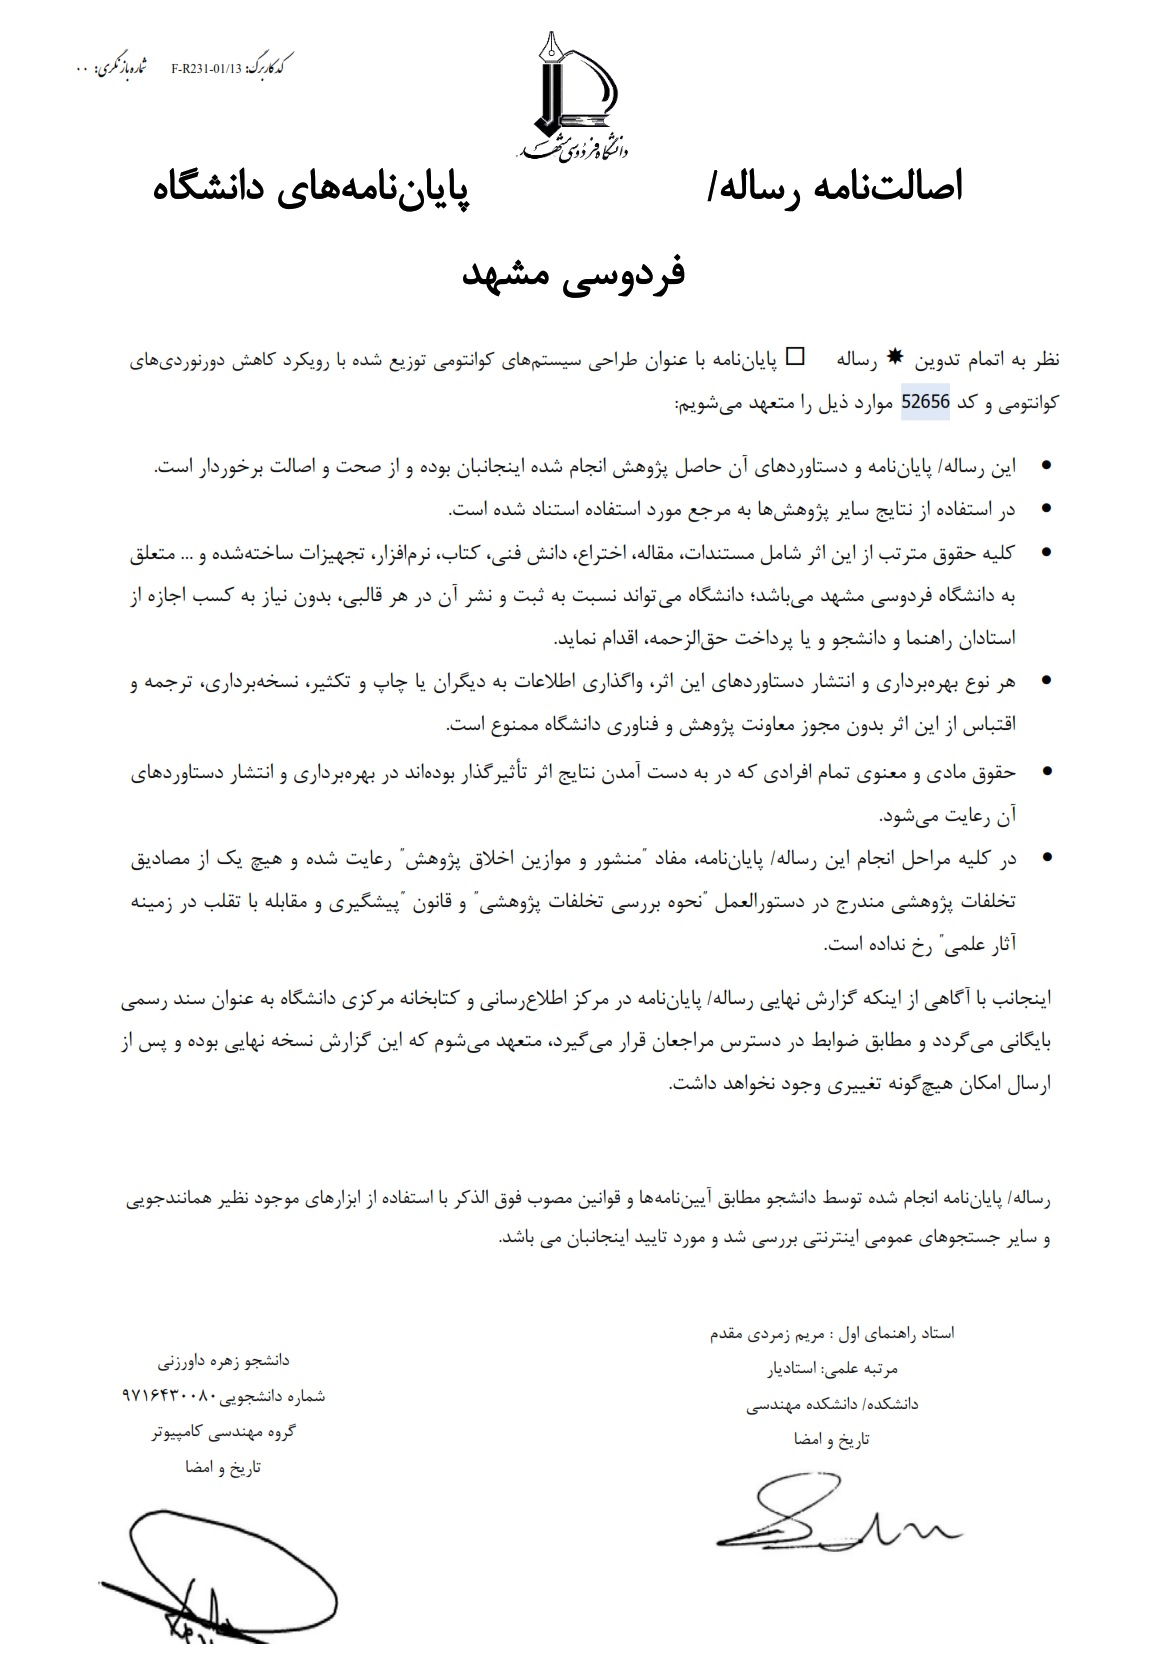
\includegraphics[scale=0.6]{esalat.jpg}\\
\end{center}
\newpage
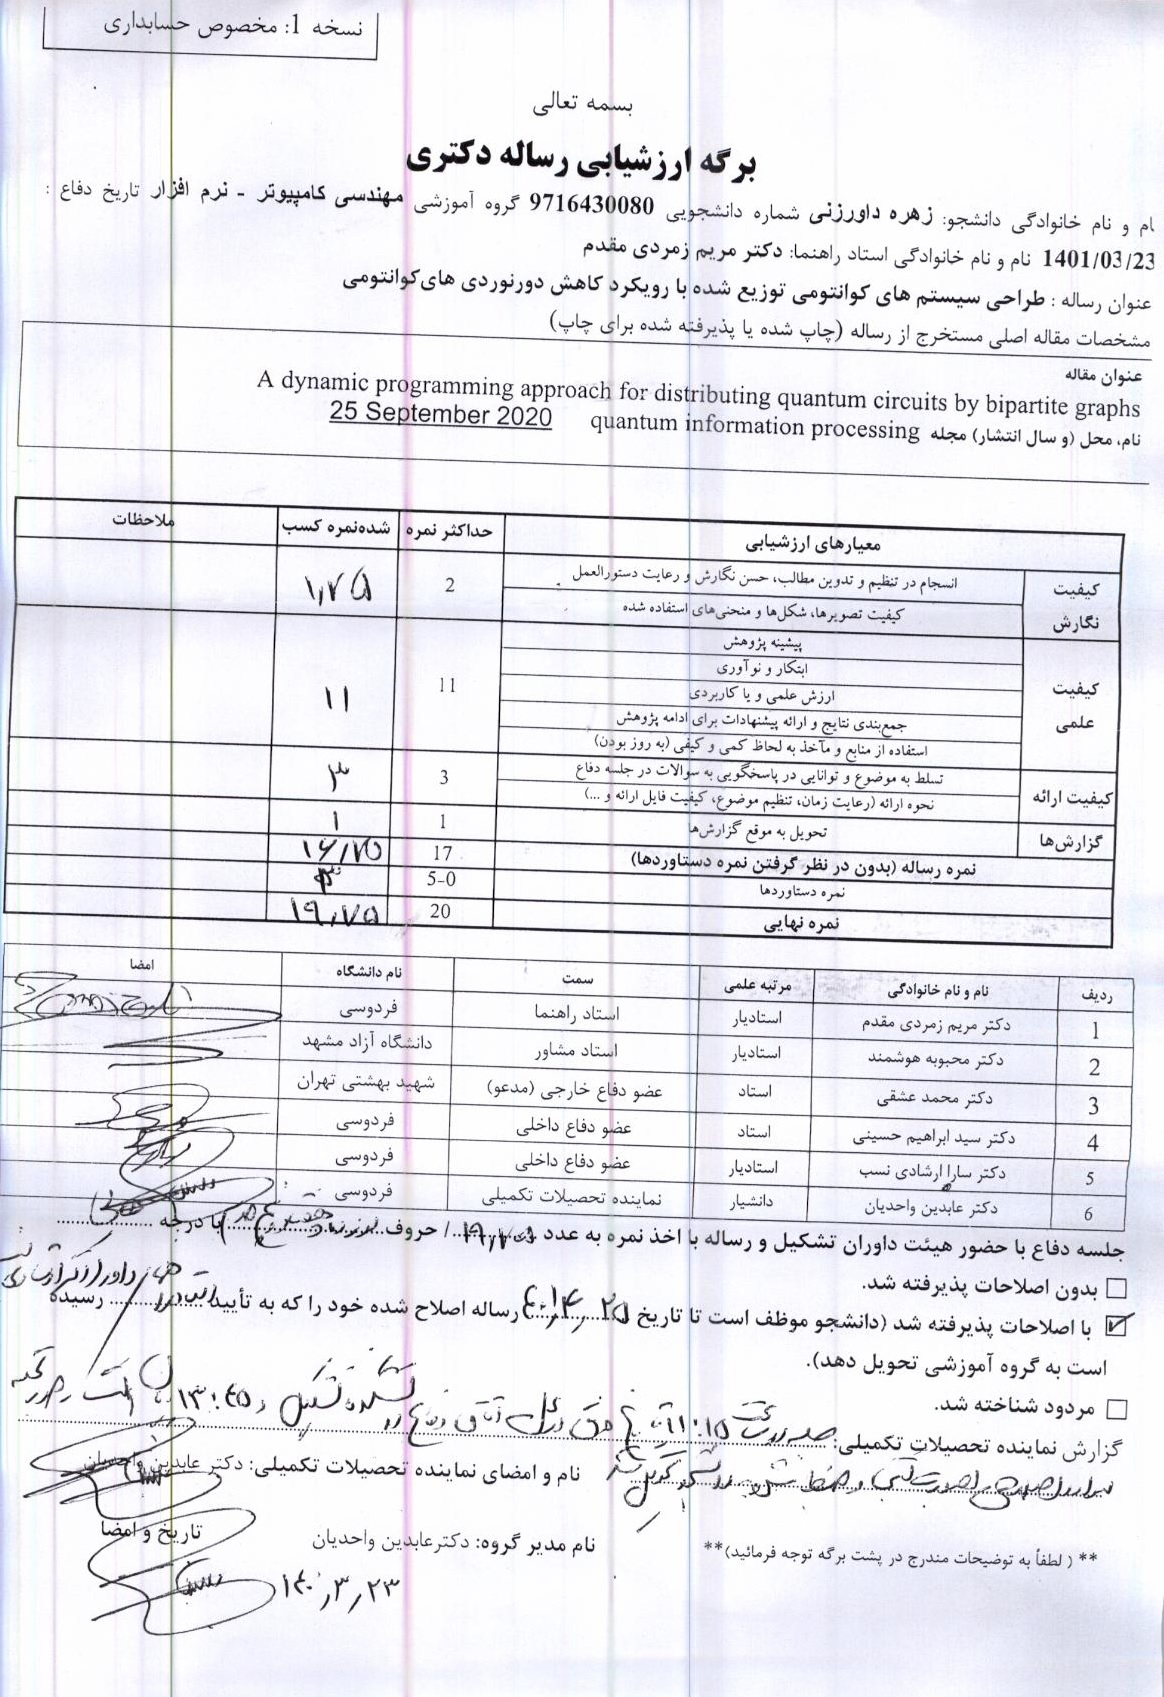
\includegraphics[scale=0.7]{arzesh.jpg}
\newpage
\KashidaOff
\begin{sols}

تقدیم به آنکه \\
\begin{center}
``تلاش مفهوم زندگی است'' 
\end{center}
\begin{flushleft}
را سرلوحه زندگی‌ام قرار داد.
\end{flushleft}

\end{sols}
\newpage
\begin{nazanint}
\begin{center}
\tashakor

منت خدای را عز و جل که طاعتش موجب قربت است و به شکر اندرش مزید نعمت.
\end{center}


در آغاز این رساله، بر خود می‌دانم از استاد بزرگوارم سرکار خانم دکتر مریم زمردی مقدم که با رهنمودهای ارزشمندشان همواره راهنما و چراغ راه من بوده‌اند، سپاس‌گزاری نمایم. حسن خلق، صبوری و همراهی این استاد گرانقدر همواره مایه‌ی آرامش و دلگرمی من در طول این دوره بوده است.

از سرکار خانم دکتر محبوبه هوشمند که با مشاوره‌های بسیار مفید و نکته‌های دلاویزشان راهگشای من در اتمام و اکمال این رساله بودند، تشکر نمایم.

همچنین، از سال‌ها زحمات و تلاش‌های بی‌دریغ کلیه اساتید محترم خویش در دانشگاه فردوسی مشهد که در تکوین دیدگاه من در دوره‌های کارشناسی، کارشناسی ارشد و دکتری نقش اساسی داشته اند، صمیمانه سپاس‌گزاری نمایم.

از پدر و مادر عزیزم، پشتیبان بی‌قید و شرط و همیشگی زندگی‌ام متشکرم.

از همسر مهربان و فرزند عزیزم که در این سال‌ها، پشتیبان، همراه و مشوق من بوده‌اند و این پژوهش بدون صبر و همراهی‌شان به سر انجام نمی‌رسید، سپاسگزارم. 
\end{nazanint}


\KashidaOn

% پایان‌نامه خود را تقدیم کنید!
\begin{acknowledgementpage}
	
	\vspace{4cm}
	
	{\nastaliq
		{\LARGE
			تقدیم به همه آنهایی که 
			\vspace{1.5cm}
			
			\hspace{3cm}
			می خواهند بیشتر بدانند
	}}
\end{acknowledgementpage}
\newpage
%%%%%%%%%%%%%%%%%%%%%%%%%%%%%%%%%%%%
% ستایش
\baselineskip=.750cm
\thispagestyle{empty}
% \KashidaOff
{\nastaliq
	خدایا...%
	\RTLfootnote{مناجاتی از دکتر علی شریعتی.}
}\\
\vspace{.5cm}\\

به من زیستنی عطا کن که در لحظه مرگ، بر بی‌ثمری لحظه‌ای که برای زیستن گذشته است، حسرت نخورم   و مُردنی عطا کن که بر بیهودگیش، سوگوار نباشم. بگذار تا آن را، خود انتخاب کنم، اما آنچنان که تو دوست می‌داری.

تو می‌دانی و همه می‌دانند که شکنجه دیدن بخاطر تو، زندانی کشیدن بخاطر تو و رنج بردن به پای تو تنها لذت بزرگ زندگی من است، از شادی توست که من در دل می‌خندم، از امید رهایی توست که برق امید در چشمان خسته‌ام می‌درخشد و از خوشبختی توست که هوای پاک سعادت را در ریه‌هایم احساس می‌کنم. نمی‌توانم خوب حرف بزنم. نیروی شگفتی را که در زیر کلمات ساده و جمله‌های ضعیف و افتاده، پنهان کرده‌ام دریاب، دریاب.

تو می‌دانی و همه می‌دانند که زندگی از تحمیل لبخندی بر لبان من، از آوردن برق امیدی در نگاه من، از برانگیختن موج شعفی در دل من، عاجز است.

تو، چگونه زیستن را به من بیاموز، چگونه مردن را خود خواهم آموخت.

به من توفیق تلاش در شکست، صبر در نومیدی، رفتن بی‌همراه، جهاد بی‌سلاح، کار بی‌پاداش، فداکاری در سکوت، دین بی‌دنیا، مذهب بی‌عوام، عظمت بی‌نام، خدمت بی‌نان، ایمان بی‌ریا، خوبی بی‌نمود، گستاخی بی‌خامی، قناعت بی‌غرور، عشق بی‌هوس، تنهایی در انبوه جمعیت، و دوست داشتن بی‌آنکه دوست بداند،  روزی کن. 

\vspace{1.5cm}
{\nastaliq
	\hspace{1cm}
	اگر تنها‌ترین تنها شوم، باز خدا هست
	\vspace{.8cm}
	
	\hspace{4.7cm}
	او جانشین همه نداشتن‌هاست...
}
%%%%%%%%%%%%%%%%%%%%%%%%%%%%%%%%%%%%
\newpage\thispagestyle{empty}
% سپاس‌گزاری
{\nastaliq
	سپاس‌گزاری...
}
\\[2cm]
سپاس خداوندگار حکیم را که با لطف بی‌کران خود، آدمی را زیور عقل آراست.


در آغاز وظیفه‌  خود  می‌دانم از زحمات بی‌دریغ استاد  راهنمای خود،  جناب آقای دکتر  سوادی، صمیمانه تشکر
و  قدردانی کنم  که قطعاً بدون 
راهنمایی‌های ارزنده‌  ایشان، این مجموعه  به انجام  نمی‌رسید.

از جناب  آقای  دکتر صدوقی یزدی که زحمت  مطالعه و مشاوره‌  این رساله
را تقبل  فرمودند و
در آماده سازی  این رساله، به نحو احسن اینجانب را مورد راهنمایی قرار دادند، کمال امتنان را دارم.

در پایان، بوسه می‌زنم بر دستان خداوندگاران مهر و مهربانی، پدر و مادر عزیزم و بعد از خدا، ستایش می‌کنم وجود مقدس‌شان را و تشکر می‌کنم از همسر و فرزندانم که با صبوری مرا در این مسیر حمایت کردند.
% با استفاده از دستور زیر، امضای شما، به طور خودکار، درج می‌شود

\newpage\clearpage

\def\title{\large{چکیده}}
\def\keyword{واژه‌های کلیدی: }
\def\abstractfa{ 
	
	امروزه شبکه‌های تطبیقی توزیع‌شده به دلیل مقیاس‌پذیری بالا، مقاومت در برابر خرابی‌ها و غیرمتمرکز بودن بسیار مورد توجه محققان در زمینه یادگیری توزیع‌شده قرار گرفته‌اند. فرآیند یادگیری الگوریتم‌های توزیع‌شده باید دارای ساختاری مشخص بوده و مبتنی بر یک مدل محاسباتی موازی انجام شود تا ارتباط بین نرم‌افزار موازی و سخت‌افزار موازی به راحتی انجام گردد. مدل محاسباتی موازی \lr{BSP} به راحتی قابل اعمال بر روی این شبکه‌ها است؛ اما در یک محیط اجرایی ناهمگن در صورت اعمال همگام‌سازی مانعی در \lr{BSP}، مساله کندکننده‌ها رخ می‌دهد و میانگین زمان انتظار گره‌ها افزایش می‌یابد. در این رساله به منظور مدیریت محیط ناهمگن، در مرحله اول با استفاده از یک روش خو‌شه‌بندی محتوایی-ساختاری گره‌های شبکه منطقه‌بندی می‌شوند. در مرحله دوم یک مدل محاسباتی موازی توسعه‌یافته به نام \lr{BSP} فدرالی یا \lr{FBSP} ارائه شده است. مدل محاسباتی پیشنهادی همانند \lr{BSP} از سه بخش مهم محاسبه، ارتباط و همگام‌سازی مانعی تشکیل شده است با این تفاوت که در \lr{FBSP}، دو نوع ابرگام منطقه‌ای و ابرگام سراسری وجود دارد. همچنین، ارتباط گره‌ها و همگام‌سازی مانعی مدل‌های تخمین‌زده شده توسط گره‌ها در دو سطح منطقه‌ای و سراسری انجام می‌شود. ارتباط دو سطحی سبب کاهش هزینه‌های ارتباطی و همگام‌سازی مانعی دو سطحی سبب مقابله با مساله کندکننده‌ها و کاهش میانگین زمان انتظار گره‌ها خواهد شد. در مرحله بعد، یک رویکرد یادگیری توزیع‌شده مبتنی بر مدل \lr{FBSP} برای حل مسائل بهینه‌سازی ارائه شد. منظور مقاوم‌سازی این رویکرد در برابر انواع نویزها و سازگاری با محیط‌های ایستا و غیرایستا، الگوریتم یادگیری توزیع‌شده انتشاری به نام \lr{RDSGD} مبتنی بر گرادیان کاهشی تصادفی معرفی شد. در نهایت، ابزار نرم‌افزاری مستقلی به نام \lr{FBSPonMPI} برای توسعه برنامه‌های توزیع‌شده در بستر شبکه‌های تطبیقی به زبان \lr{C} و پایتون ارائه شده است که سریع و مستقل از سخت‌افزار است. تحلیل همگرایی و کارایی رویکرد پیشنهادی در حالت میانگین و مربع میانگین و بررسی تاثیر توپولوژی تصادفی در شبکه و خطا کمی‌سازی انجام شده است. جهت تصدیق نتایج تحلیلی بدست آمده، رویکرد پیشنهادی با استفاده از تعدادی معیار ارزیابی با سایر رویکرد‌ها مقایسه شده است. رویکرد مبتنی بر مدل \lr{FBSP} بر روی مساله بهینه‌سازی شناسایی سیستم و پیش‌بینی بازار سهام مورد ارزیابی قرار گرفت. رویکرد پیشنهادی در حضور نویزهای مختلف و در محیط‌های ایستا و غیرایستا نسبت به سایر روش‌ها مقاوم‌تر و سازگارتر است. نتایج بدست آمده نشان می‌دهند که رویکرد پیشنهادی موفق به کاهش $36.9\%$ در میانگین زمان انتظار و کاهش $58\%$ در میانگین تعداد ارتباطات با حفظ نرخ همگرایی و دقت یادگیری شده است.
}
\def\keywordfa{شبکه‌های تطبیقی‌ توزیع‌شده، یادگیری توزیع‌شده، مدل‌ محاسباتی موازی، مدل محاسباتی همگام مانعی فدرالی، ابرگام منطقه‌ای، ابرگام سراسری}

\begin{center}
\title
\end{center}
\abstractfa

\textbf{واژه‌های کلیدی:}
\keywordfa
%\setcounter{page}{1}

\renewcommand{\listfigurename}{\LARGE{فهرست شکل‌ها}}
\renewcommand{\listtablename}{\LARGE{فهرست جدول‌ها}}
%\addtocontents{toc}{\textbf{عنوان}~\hfill\textbf{صفحه}\par\rule{\linewidth}{1pt}\par}
%\addtocontents{lof}{\textbf{عنوان}~\hfill\textbf{صفحه}\par\rule{\linewidth}{1pt}\par}
%\addtocontents{lot}{\textbf{عنوان}~\hfill\textbf{صفحه}\par\rule{\linewidth}{1pt}\par}
%\renewcommand{\cfttoctitlefont}{\hspace*{\fill}\Huge\bfseries}
%\renewcommand{\cftaftertoctitle}{\hspace*{\fill}}
%\renewcommand{\cftlottitlefont}{\hspace*{\fill}\Huge\bfseries}
%\renewcommand{\cftafterlottitle}{\hspace*{\fill}}
%\renewcommand{\cftloftitlefont}{\hspace*{\fill}\Huge\bfseries}
%\renewcommand{\cftafterloftitle}{\hspace*{\fill}}

\tableofcontents
\newpage
\listoffigures
\listoftables

\newpage

\mainmatter


\setcounter{page}{1}
\pagenumbering{arabic}

\chapter{مقدمه}
\newpage
در این فصل ابتدا تعریفی از مساله و سپس چالش‌های موجود در این حوزه مطرح می‌گردد. به دنبال چالش‌های مطرح شده در بخش‌های بعدی، اهداف دنبال شده در این رساله و جنبه‌ جدید بودن و نوآوری‌های رساله بیان می‌شود. در انتهای این فصل به ساختار رساله پرداخته شده است.   
‎\renewcommand{\baselinestretch}{2}\normalsize‎
\label{Introduction}
\section{تعریف مساله}
امروزه با افزایش حجم داده‌های پردازشی و محاسبات در بسیاری از کاربردها، چالش‌های بسیاری در فرآیند یادگیری الگوریتم‌های توزیع‌شده مطرح می‌شود. در یک شبکه تطبیقی توزیع‌شده\footnote{\lr{Distributed Adaptive Networks}} با محاسبات سنگین  یا داد‌های ذاتاً توزیع‌شده، موازی‌سازی فرآیند یادگیری و ایجاد یک مدل منسجم در کل شبکه اصلی‌ترین موضوع می‌باشد. به منظور تسریع عملیات و مدیریت راحت‌تر بخش‌های محاسبات و ارتباطات، یادگیری موازی باید تحت یک مدل محاسباتی موازی از جمله  \lr{PRAM}، \lr{LogP}، \lr{BSP} و \lr{MapReduce} پیاده‌سازی شود. هر الگوریتم موازی طراحی شده بر اساس مدل محاسباتی \lr{BSP} شامل تعدادی ابرگام با سه بخش مجزای محاسبه، ارتباط و همگام‌سازی مانعی می‌باشد. مقیاس‌پذیری، عملکرد بالا، استفاده آسان، پیش‌بینی زمان اجرا الگوریتم طراحی شده بر اساس آن و داشتن مدل برنامه‌نویسی از ویژگی‌های مهم این مدل محاسباتی است. مدل \lr{BSP} به راحتی قابل اعمال بر روی شبکه‌های تطبیقی توزیع‌شده است. این شبکه‌ها مقیاس‌پذیری بالایی دارند و در برابر خرابی‌ها مقاومت بوده و نیاز به سرور مرکزی ندارند. 

در یک محیط محاسباتی ناهمگن، گره‌های شبکه از لحاظ قدرت پردازشی و ارتباطی متفاوت خواهند بود و در صورت اعمال همگام‌سازی مانعی در مدل \lr{BSP}، مساله کندکننده‌ها رخ می‌دهد و میانگین زمان انتظار گره‌ها افزایش می‌یابد. در غیر این صورت، گره‌های کند می‌توانند شکاف تکرار را در بین گره‌های شبکه به تدریج افزایش داده و در نتیجه دقت یادگیری را کاهش دهند. به منظور همگرایی سریع و دقت یادگیری بالا، نیاز است که همگام‌سازی گره‌ها انجام شود اما باید سازگار با محیط‌های محاسباتی ناهمگن باشد.

با پیشرفت سریع فناوری‌های شبکه‌ای و ارتباطی، شبکه‌های توزیع‌شده‌ای که رایانه‌های شخصی، تلفن‌های همراه، حسگرها و محرک‌ها را به هم متصل می‌کنند، چهارچوب اصلی شبکه‌های ارتباطی و کنترل داده‌ها را تشکیل می‌دهند. در این شبکه‌ها نیاز به یادگیری توزیع‌شده زمانی به وجود می‌آید که یک هدف جهانی باید از طریق همکاری محلی بر روی تعدادی از عامل‌های به هم پیوسته محقق شود. این مساله در بسیاری از زمینه‌های مهم از جمله تخمین توزیع شده، یادگیری ماشین توزیع شده، تخصیص منابع و همچنین در مدل‌سازی رفتار دسته جمعی و ازدحامی توسط شبکه‌های بیولوژیکی رخ می‌دهد. شبکه‌های تطبیقی توزیع‌شده برای انجام وظایف پردازش و بهینه‌سازی اطلاعات غیرمتمرکز و مدل‌سازی انواع رفتارهای خودسازمان‌یافته و پیچیده‌ای که در طبیعت با آن مواجه هستیم، مناسب می‌باشند \cite{Zhao2014}. یک شبکه‌ تطبیقی توزیع‌شده شامل مجموعه‌ای از فیلترهای وفقی\footnote{\lr{Adaptive Filters}} یا عامل‌های یادگیری است. عامل‌ها از طریق توپولوژی اتصال به یکدیگر متصل می‌شوند و از طریق تعاملات محلی با یکدیگر همکاری می‌کنند تا مسائل بهینه سازی، تخمین و یا استنتاج توزیع‌شده را در زمان واقعی حل کنند. انتشار مداوم اطلاعات در سراسر شبکه توزیع‌شده، عامل‌ها را قادر می‌سازد تا عملکرد خود را در رابطه با جریان داده‌ها و شرایط شبکه تطبیق دهند. همچنین منجر به بهبود عملکرد سازگاری و یادگیری نسبت به عامل‌های غیرهمکار می‌شود. 

شبکه‌های تطبیقی توزیع‌شده جز دسته شبکه‌های غیرمتمرکز\footnote{\lr{Decentralized network}} می‌باشند و  با شبکه‌های متمرکز\footnote{\lr{Centralized network}} که یک گره مرکزی، به کلیه گره‌های شبکه متصل است و وظیفه تجمیع و پراکندگی اطلاعات محلی را بر عهده دارد، متفاوت می‌باشند. مقیاس‌پذیری و مقاومت در برابر خرابی گره‌ها و یال‌ها از ویژگی‌های مهم این شبکه‌ها است. همچنین اثربخشی و کارایی هر پیاده‌سازی تطبیقی توزیع‌شده در این شبکه‌ها به حالت همکاری بین عامل‌ها بستگی دارد. سه راه‌حل همکاری غیرمتمرکز مفید، از جمله استراتژی‌ اجماع\footnote{\lr{Consensus}}، استراتژی افزایشی\footnote{\lr{Incremental}} و استراتژی‌ انتشار\footnote{\lr{Diffusion}}، برای این منظور توسعه داده شده است \cite{Sayed2013} ، \cite{SayedBook}. روش همکاری انتشار نسبت به تغییرات محیط تطبیق‌پذیرتر از روش همکاری اجماع است و همانند روش همکاری افزایشی نیازی به یافتن دور در شبکه ندارد و هر گره می‌تواند با همه همسایگانش ارتباط داشته باشد و تخمین‌های دریافتی آنها را با داده‌های محلی خود تلفیق نماید. روش انتشار نسبت به اجماع دارای مزیت همگرایی سریع‌تر و رسیدن به میانگین مربع انحراف کمتر است \cite{Sayed2013,Sayed2014}. به طور خلاصه، روش‌های همکاری انتشار مقیاس‌پذیر، قوی، کاملاً توزیع‌شده هستند و به شبکه‌ها انطباق و توانایی یادگیری در زمان واقعی را می‌دهند. علاوه‌بر این، در مقاله \cite{Sayed2012} نشان داده شده است که روش‌های انتشار پایدارتر هستند و پایداری آن‌ها نسبت به توپولوژی شبکه غیر حساس است و منجر به بهبود کارایی و حالت پایدار در شبکه‌های تطبیقی می‌شوند.

الگوریتم‌های تطبیقی بسیاری وجود دارند که می‌توانند برای محاسبه و تخمین بردار پارامتر مسائل بهینه‌سازی مورد نظر در شبکه‌های تطبیقی توزیع‌شده مورد استفاده قرار بگیرند. برخی الگوریتم‌ها دقیق‌تر و گاهی پیچیده‌تر از سایرین هستند و برخی ساختاری ساده و در عین حال موثری دارند. بسیاری از این الگوریتم‌های تطبیقی مبتنی بر روش‌های گرادیان کاهشی\footnote{\lr{Gradient Descent}} می‌باشند. گرادیان کاهشی به روش‌های کمینه‌سازی اشاره دارد که محدود به استفاده از یک تابع هزینه\footnote{\lr{Cost function}}  خاصی نیستند. در حالیکه الگوریتم تطبیقی \lr{LMS} نوع خاصی از گرادیان کاهشی است که از تابع هزینه میانگین مربع خطا استفاده می‌کند. 

روش‌های گرادیان کاهشی\footnote{\lr{Gradient Descent}} الگوریتم‌ یادگیری مناسبی برای حل مسائل پیش‌بینی خطی بزرگ می‌باشند و یکی از محبوب‌ترین الگوریتم‌ها برای بهینه‌سازی و با اختلاف زیاد، پرکاربردترین روش برای بهینه‌سازی شبکه‌های عصبی است\cite{Bo2010}. روش‌های گرادیان کاهشی متفاوتی بر اساس حجم داده‌ استفاده شده برای محاسبه‌ی گرادیان تابع هدف \footnote{\lr{Cost function}} ارائه شده است. در روش گرادیان کاهشی تصادفی (\lr{SGD})\footnote{\lr{Stochastic Gradient Descent}} به ازای هر داده ورودی یک گام به‌روزرسانی بر روی بردار پارامتر انجام می‌شود. این روش تصادفی تغییرات را با واریانس بالایی ایجاد می‌کند که باعث می‌شود تابع هدف به شدت نوسان کند. برای حل این مشکل می‌شود به ازای هر دسته \footnote{\lr{Batch}} از داده‌های ورودی، یک گام گرادیان انجام شود. در این حالت واریانس تغییرات پارامترها کمتر می‌شود، در نتیجه نرخ همگرایی سریع‌تر خواهد بود. اندازه دسته می‌تواند برای کاربردهای مختلف متفاوت باشد\cite{We2018}.  

الگوریتم‌های گرادیان کاهشی تصادفی مرتبه دوم که جز این دسته از الگوریتم‌ها هستند، برای تخمین تطبیقی بردار پارامترهای مساله بهینه‌سازی در این رساله به‌کار گرفته می‌شوند. زیرا این الگوریتم‌ها برای هر دو نوع یادگیری برخط و برون‌خط کاربرد داشته و در حین اینکه حساس به ترتیب پردازش داد‌ه‌های ورودی نیستند، از دقت بالایی نیز برخوردار می‌باشند. با این اوصاف انتخاب مناسبی برای استفاده در شبکه‌های تطبیقی توزیع شده می‌باشند.

امروزه با افزایش حجم داده‌های پردازشی و نیاز به محاسبات سنگین در بسیاری از کاربردها، چالش‌های فراوانی در فرآیند یادگیری الگوریتم‌های تطبیقی مطرح شده است. در یک شبکه تطبیقی توزیع‌شده با حجم عملیات محاسباتی بالا یا حجم داده‌های پردازشی بالا، موازی‌سازی فرآیند آموزش و ایجاد یک مدل منسجم در کل شبکه  مهمترین مساله در فرآیند یادگیری خواهد بود. یادگیری موازی باید تحت یک مدل یا چارچوب محاسباتی موازی پیاده‌سازی و اجرا شود. از جمله این مدل‌های محاسباتی می‌توان به \lr{PRAM}، \lr{LogP}، \lr{BSP} و چارچوب محاسباتی \lr{MapReduce} اشاره کرد. مدل محاسباتی \lr{PRAM} (ماشین موازی با دستیابی تصادفی)\footnote{\lr{Parallel Random Access Machine}} \cite{Ja1992} یک مدل حافظه اشتراکی است که ارتباط بین پردازنده‌ها از طریق حافظه اشتراکی انجام می‌شود. به این دلیل که هزینه ارتباطات در این مدل بیشتر از هزینه محاسباتی است و تعداد پردازنده‌ها محدود است، این مدل برای پیاده‌سازی همه‌منظوره در سخت‌افزار مناسب نیست. چارچوب محاسباتی نگاشت-کاهش یا \lr{MapReduce} توسط گوگل\cite{De2008} توسعه یافته و برای حل برخی مسائل غیر پیش پا افتاده در زمینه‌های پردازش داده، داده‌کاوی و تجزیه و تحلیل گراف استفاده شده است. یک الگوریتم نگاشت-کاهش شامل تعدادی دور است که هر دور از یک فاز نگاشت و یک فاز کاهش تشکیل شده است. در این مدل ماشین‌ها تنها مجاز به برقراری ارتباط با ماشین پردازنده اصلی می‌باشند و حافظه اولیه محلی هر ماشین قبل از هر همگام‌سازی به طور کامل پاک می‌شود. در نتیجه برای پیاده‌سازی الگوریتم‌های تکرارشونده مناسب نمی‌باشد. مدل محاسباتی \lr{BSP} (موازی‌سازی همگام مانعی)\footnote{\lr{Bulk Synchronous Parallel}} \cite{Va1990} تعمیمی از مدل محاسباتی \lr{PRAM} است که توسط پروفسور \lr{L. G. Valiant } از دانشگاه هاروارد در سال 1990 پیشنهاد شده است. در سال‌های بعد، این مدل بوسیله پروفسور \lr{McCall} و \lr{Valiant} توسعه یافته است که به عنوان یک مدل پل برای محاسبات موازی برای سیستم‌هایی با حافظه توزیع‌شده کاربرد دارد. مدل محاسباتی \lr{BSP} شامل بخش‌های زیر می‌باشد:
\begin{itemize}
	\item
	مجموعه‌ای از کامپیوترها که هر یک دارای حافظه محلی می‌باشند
	\item 
	یک شبکه ارتباطی که پیام‌ها را از نقطه‌ای به نقطه دیگر انتقال می‌دهد
	\item 
	مکانیزمی که همگام‌سازی همه یا گروهی از پردازنده‌ها را انجام می‌دهد. 
\end{itemize}
برنامه‌های \lr{BSP} به صورت دنباله‌ای از ابرگام‌ها\footnote{\lr{Superstep}} نوشته می‌شوند. هر ابرگام از سه بخش اصلی تشکیل شده است: محاسبات بر روی داده‌های محلی، ارسال و دریافت پیام به منظور دسترسی به داده‌های غیرمحلی و همگام‌سازی مانعی به منظور تکمیل همه عملیات ارتباطی و از سرگیری محاسبات روی داده‌های محلی یا داده‌هایی که از طریق تبادل پیام به یک پردازنده رسیده‌اند. زمان اجرای یک رویکرد یا الگوریتم طراحی شده تحت مدل محاسباتی \lr{BSP} را می‌توان با استفاده از چهار پارامتر تاخیر شبکه، سرعت  پردازنده‌ها، تعداد پردازنده‌ها و نرخ راندمان ارتباطات پیش‌بینی کرد. 

این مدل محاسباتی منطبق با نیازها و ویژگی‌های شبکه‌های تطبیقی توزیع‌شده است و برای پیاده‌سازی الگوریتم‌های یادگیری تکرارشونده آن‌ها مناسب می‌باشد. مکانیزم همگام‌سازی مانعی در این مدل سبب می‌شود که در انتهای هر ابرگام تمام گره‌های شبکه عملیات ارتباطی و محاسباتی‌ خود را به اتمام رسانده و سپس  محاسبات ابرگام بعدی بر روی داده‌های محلی یا داده‌هایی که از طریق تبادل پیام به گره رسیده‌اند، انجام شوند. گره‌های شرکت‌کننده در یک شبکه تطبیقی توزیع‌شده ممکن است از لحاظ قدرت پردازشی و ارتباطی با یکدیگر متفاوت باشند. در نتیجه با یک محیط توزیع‌شده ناهمگن مواجه خواهیم بود که برخی از گره‌ها عملیات ارتباطی و یا محاسباتی را سریع‌تر انجام خواهند داد و به اجبار باید منتظر گره‌های کندتر در فرایند یادگیری بمانند تا پس از پایان عملیات آن گره‌ها بتوانند ابرگام بعدی را آغاز کنند. در چنین حالتی، مکانیزم همگام‌سازی مانعی سبب کاهش کارایی الگوریتم یادگیری و افزایش زمان انتظار گره‌های سریع‌تر در شبکه خواهد شد.

در این رساله یک رویکرد یادگیری توزیع‌شده برای تخمین پارامترهای مساله بهینه‌سازی در شبکه‌های تطبیقی توزیع‌شده ارائه می‌شود که مبتنی بر یک مدل محاسباتی توسعه‌یافته به نام \lr{BSP} فدرالی (\lr{FBSP}) است. همگام‌سازی گره‌های شبکه در این رویکرد با استفاده از یک تکنیک همگام‌ فدرالی انجام خواهد شد. در این تکنیک گره‌های شبکه در دو سطح منطقه‌ای و سراسری همگام می‌شوند. رویکرد پیشنهادی در دو مرحله اصلی برون‌خط و برخط اجرا می‌شود. مرحله برون‌خط که مرحله پیش‌پردازش نیز نامیده می‌شود، شامل دو بخش رصدکردن  شبکه و منطقه‌بندی آن است. در بخش رصد کردن شبکه، توان پردازشی هر گره محاسبه می‌شود. در بخش منطقه‌بندی شبکه، دسته‌بندی گره‌ها براساس فاصله گره‌ها از همدیگر، توان پردازشی و میزان اعتماد بین گره‌ها انجام می‌شود. در مرحله برخط، فرآیند یادگیری توزیع‌شده تحت مدل محاسباتی پیشنهادی \lr{FBSP} بر روی شبکه تطبیقی که در مرحله پیش‌پردازش منطقه‌بندی شده است، اجرا خواهد شد. مدل محاسباتی پیشنهادی همانند مدل \lr{BSP} شامل سه بخش مهم محاسبه، ارتباط و همگام‌سازی مانعی می‌باشد. با این تفاوت که مرحله ارتباط و همگام‌سازی مانعی در مدل \lr{FBSP} بر اساس یک روش منطقه‌بندی‌ انجام می‌شود که متناسب با ویژگی‌های شبکه‌ تطبیقی توزیع‌شده است. این روش منطقه‌بندی سبب می‌شود هزینه ارتباطات بین گره‌ها در زمان اجرا کاهش یابد و از وقوع مساله کندکننده‌ها جلوگیری به عمل می‌آید. در نتیجه زمان انتظار گره‌ها در شبکه کاهش خواهد یافت.

مساله کندکننده‌ها به یکی از دو دلیل 1) وجود گره‌های کند در بین گره‌های شبکه و 2) عدم توازن بار در بین گره‌‌ها، رخ خواهد داد. در حالتی که داد‌ه‌های پردازشی در شبکه توزیع‌شده از نوع ویدیو یا هر داده دیگری با اندازه‌های متفاوت باشد، عدم توازن بار را در گره‌ها خواهیم داشت که سبب می‌شود برخی از گره‌ها با اندازه داده یا اندازه ویدیو کوچک‌تر محاسبات‌شان زودتر تمام شود و منتظر سایر گره‌ها برای اتمام کارشان بمانند. در صورتی‌که توزیع بار بین گره‌ها به صورت یکسان انجام شده باشد، با افزایش تعداد گره‌هاي شرکت‌کننده در محیط توزیع‌شده، احتمال حضور گره‌های کند و گره‌هایی با قدرت پردازشی  و قدرت ارتباطی متفاوت در شبکه بسیار بالا خواهد رفت و یک محیط ناهمگن داریم. این موضوع افزایش زمان انتظار گره‌های سریع‌تر را نتیجه خواهد داد. در نتیجه زمان انتظار و زمان بیکار ماندن گره‌ها افزایش پیدا می‌کند.

رویکرد یادگیری توزیع‌شده پیشنهادی که یک رویکرد غیرمتمرکز است در واقع یادگیری مشارکتی را پیاده‌سازی می‌نماید. راه‌حل‌های غیرمتمرکز پتانسیل بالایی برای نسل پنجم (\lr{5G}) صنعتی از جمله رانندگی مشارکتی در وسایل نقلیه خودکار متصل و روباتیک مشارکتی در تولید هوشمند دارند. رویکرد پیشنهادی برای دو کاربرد شناسایی سیستم و پیش بینی بازار بورس مورد بررسی قرار گرفته است. کاربرد این رویکرد به این دو مساله محدود نمی شود بلکه قابل اعمال بر روی کلیه مسائل یادگیری با هدف تخمین پارامترها و مسائل پیش‌بینی مختلف خواهد بود. در مساله شناسایی سیستم هدف شناسایی مدل ریاضی سیستم ناشناخته با استفاده از داده‌های اندازه‌گیری‌شده است. در بازار بورس روزانه با حجم زیادی از اطلاعات و تراکنش‌ها مواجهه خواهیم بود و گاها نیاز به تحلیل‌های آنی و سریع وجود دارد تا‌‌ با پیش‌بینی‌های دقیق امکان انجام معامله‌های هوشمندانه و پرسود میسر شود. مساله پیش‌بینی بازار بورس سهام از جمله مسائلی است که رویکرد یادگیری توزیع‌شده پیشنهادی قادر است پیش‌بینی را با دقت بالا و نرخ خطا پایین انجام دهد.  

\section{چالشهای موجود}
در این بخش به بررسی چالش‌های موجود در مساله که به موجب آنها سمت و سوی اصلی این رساله شکل گرفته است، پرداخته شده است:
\begin{itemize}
	\item
	%1
	با رشد سریع حجم داده‌ها و محاسبات، فرآیند یادگیری در شبکه‌های تطبیقی توزیع‌شده نیازمند یک ساختار استاندارد موازی با تسریع هدفمند است. براساس بررسی‌های انجام‌شده در بخش قبل، یکی از چالش‌های اساسی در شبکه‌های تطبیقی توزیع‌شده عدم ارائه یک رویکرد یادگیری توزیع‌شده مبتنی بر یک مدل محاسباتی موازی برای این نوع از شبکه است که قادر باشد تعاملات بین گره‌ها را به خوبی در دنیای واقعی مدیریت نماید و متناسب با خصوصیات و نحوه ارتباطات و تعاملات گره‌ها در این نوع شبکه‌ها باشد و قابلیت پیش‌بینی زمان اجرا را در زمان پیاده‌سازی رویکرد داشته باشد.
	
	‌\item 
	%2
	هنگامی‌که پیاده‌سازی شبکه‌های تطبیقی توزیع‌شده به یک محیط بزرگ و ناهمگن گسترش می‌یابد، ناهمگنی قطعی در سخت‌افزار و قدرت محاسباتی گره‌ها را دیگر نمی‌توان نادیده گرفت. همچنین، در محاسبات ناهمگن توزيع‌شده مانند رایانش ابری، سرعت پردازش گره‌ها از لحاظ محاسباتی يا ارتباطی اغلب متفاوت است، از اين رو الگوريتم‌هاي یادگیری همگام در اين محيط‌ها سبب كاهش نرخ همگرايي و در بعضی مواقع واگرايي مي‌شوند. یکی دیگر از چالش‌های موجود، ارائه یک رویکرد یادگیری توزیع‌شده سازگار با محیط‌های ناهمگن و بارهای ‌کاری نامتوازن در شبکه است. 
	
	\item 
	%3
	در روش‌های مختلف یادگیری توزیع‌شده، همگام‌سازی گره‌ها بخش اصلی فرآیند یادگیری را تشکیل می‌دهد و تاثیر به‌سزایی بر روی مقیاس‌پذیری بهتر در محیط‌های توزیع‌شده ناهمگن دارد. در نتیجه، نیاز به یک تکنیک همگام‌سازی مدل‌ها در چنین محیط‌هایی به شدت احساس می‌شود که هم نرخ‌ همگرایی مناسبی داشته باشد و هم هزینه ارتباطات آن قابل قبول باشد. این شبکه‌ها که غيرمتمركز بوده و فاقد سرور پارامتري براي همگام‌سازي و تجميع مدل‌هاي برآورده شده هستند، نیازمند روشي براي همگام‌سازي با توجه به مساله و كاربرد می‌باشند. به طور معمول، همگام‌سازی مدل‌ها در گره‌هاي شبكه در انتهای هر تكرار انجام می‌شود. البته اجرای زياد همگام‌سازی باعث افزایش زمان یادگیری و کاهش بازدهی می‌گردد.

	‌\item 
	%4
	از دیگر چالش‌های موجود در رویکردهای توزیع‌شده، برقراری مصالحه بین پیچیدگی ارتباطی و نرخ همگرایی است. در یادگیری توزیع‌شده محاسبات در چند گره اجرا می‌شوند ولی سرعت اجرا الزاماً برابر با تعداد گره‌ها ضربدر سرعت یک گره نیست و این به دلیل هزینه ارتباطات بین گره‌ها است. در نتیجه، در طراحی تکنیک‌های همگام‌سازی توجه به میزان و پیچیدگی ارتباطات و هزینه‌های آن در مقابل حفظ همگرایی از الزامات کار می‌باشد.
	
		\item 
		%5
	‌یکی از چالش‌‌ها عدم وجود یک الگوریتم انتشاری تطبیقی همه منظوره برای شبکه‌های تطبیقی توزیع‌شده است که علاوه بر مقاوم بودن در برابر انواع نویزهای محیطی و محیط‌های ایستا و غیرایستا، قابلیت این را نیز داشته باشد که در محیط‌های برون‌خط و برخط قابل اجرا باشد و نسبت به ترتیب ورود داده‌ها حساس نباشد.
\end{itemize}
در این رساله سعی  شده است با مطالعات دقیق و بررسی‌های همه‌جانبه بر روی خصوصیات شبکه‌های تطبیقی توزیع‌شده، یک رویکرد یادگیری توزیع‌شده برای این شبکه‌ها بر پایه یک مدل محاسباتی توسعه‌یافته ارائه شود که گره‌ها به صورت موازی اقدام به یادگیری توزیع‌شده انتشاری نموده و بر اساس تکنیک همگام‌سازی مناسبی اقدام به‌روزرسانی مدل خویش نمایند.

\section{اهداف مساله}
با توجه به چالش‌های بیان شده در بخش قبل، در این رساله سعی شده است رویکردی ارائه شود تا فرآیند یادگیری و تخمین پارامتر را در یک شبکه تطبیقی توزیع‌شده‌ ناهمگن تحت یک مدل محاسباتی موازی توسعه‌یافته انجام دهد، به گونه‌ای که اهداف زیر مقرر گردد:
\begin{itemize}
	\item
	%1
	با توجه به چالش‌های موجود، ارائه یک مدل محاسباتی موازی جهت اجرا در شبکه‌های تطبیقی توزیع‌شده‌ به شدت مورد نیاز است. در این رساله، یکی از اهداف اصلی ارائه مدلی محاسباتی موازی متناسب با ویژگی‌های این شبکه‌ها برای حل مسائل بهینه‌سازی در یک محیط ناهمگن است. ناهمگنی در یک محیط محاسباتی به دلایل تفاوت در قدرت پردازشی و ارتباطی گره‌های شبکه یا  بارهای کاری نامتوازن رخ می‌دهد.	
	\item 
	%2
	با توجه به اینکه در یک محیط اجرایی ناهمگن ممکن است گره‌های شبکه از لحاظ قدرت پردازشی و ارتباطی متفاوت باشند، یکی از اهداف مورد نظر در این رساله استفاده از یک روش خوشه‌بندی محتوایی-ساختاری برای منطقه‌بندی گره‌های شبکه است. در این راستا، منطقه‌بندی گره‌ها در شبکه بر اساس یک ماتریس شباهت انجام می‌شود که با استفاده از ویژگی‌های ساختاری و محتوایی گره‌ها مقداردهی می‌شود. در این رساله، ویژگی‌های ساختار هر گره شامل فاصله آن گره از سایر گره‌ها و ضریب اعتماد به داده‌های دریافتی از گره‌های دیگر است و ویژگی‌های محتوایی هر گره شامل قدرت پردازشی و ارتباطی آن گره می‌باشد.  

	\item 
	%3
	با توجه به اینکه یک شبکه تطبیقی توزیع‌شده در واقع یک شبکه غیرمتمرکز و نظیر-به-نظیر با قابلیت تعامل و همکاری بین گره‌ها است، همگام‌سازی مدل‌های تخمین‌زده شده توسط گره‌ها امری بسیار مهم و موثر در کارایی و همگرایی مدل‌ها است و ناهمگنی محیط اجرا می‌تواند سبب افزایش زمان انتظار گره‌ها در شبکه در حین فرآیند یادگیری و کاهش دقت تخمین و گاها سبب عدم همگرایی شود. به همین منظور، لازم است در هر مرحله یادگیری، همگام‌سازی مانعی در محیط اجرایی ناهمگن در یکی از دو سطح منطقه‌ای یا سراسری انجام می‌شود. انجام همگام‌سازی مانعی دو سطحی علاوه بر افزایش نرخ همگرایی، سبب مقابله با مساله کندکننده‌ها و کاهش زمان انتظار گره‌ها می‌شود. 
	\item 
	%4
	یکی از چالش‌ها برقراری مصالحه بین پیچیدگی ارتباطی و نرخ همگرایی است. یکی از اهداف این رساله کاهش پیچیدگی و میزان ارتباطات گره‌ها در رویکرد یادگیری توزیع‌شده است. بدین منظور، به دنبال این هستیم که ارتباط گره‌ها بر اساس منطقه‌بندی گره‌ها در دو سطح منطقه‌ای و سراسری انجام شود. گره‌هایی که بر اساس معیارهای خوشه‌بندی در یک منطقه مشابه قرار می‌گیرند، تنها با گره‌های همسایه در آن منطقه ارتباط برقرار می‌کنند و مدل‌ پارامتری تخمین‌زده خویش را با گره‌ها تبادل خواهند کرد. اما در سطح سراسری، گره‌ها با همسایه خود در کل شبکه به ارتباط و تبادل اطلاعات می‌پردازند. منطقه‌بندی گره‌ها و انجام ارتباطات در دو سطح سبب کاهش هزینه‌های ارتباطی نیز خواهد شد. 
	\item 
	%5
	حضور انواع مختلف نویز در محیط‌های توزیع‌شده غیر قابل اجتناب است. یکی از اهداف مورد نظر در این رساله، ارائه الگوریتم یادگیری توزیع‌شده‌ای است که در مقابل انواع نویزهای گاوسی و غیرگاوسی مقاوم باشد. همچنین کارایی و همگرایی الگوریتم ارائه شده هم در محیط‌های ایستا و هم غیرایستا قابل قبول باشد. بدین منظور یک الگوریتم یادگیری توزیع‌شده انتشاری ارائه خواهد شد که در انواع محیط‌ها و در برابر انواع نویزها مقاوم خواهد بود. 
	\item 
	%6
	یکی از اهداف دیگر که در این رساله به دنبال آن هستیم، ارائه ابزاری یکپارچه با استفاده آسان برای برنامه‌های توزیع‌شده در بستر شبکه‌های تطبیقی است که مستقل از سخت‌افزار و سریع بوده و قابل اجرا بر روی کلیه ماشین‌ها باشد. 
	
\end{itemize}


\section{جنبه جدید بودن و نوآوری}

جنبه‌های جدید بودن و نوآوری راهکار پیشنهادی به شرح زیر می‌باشد:

\begin{itemize}
	\item
	%1
	رویکرد یادگیری توزیع‌شده دو مرحله‌ای: یک شبکه‌ تطبیقی توزیع‌شده در واقع یک گراف نظیر-به-نظیر است که تمام گره‌ها در سطح برابری از مسئولیت قرار دارند و هیچ گره مرکزی به منظور کنترل و مدیریت فعالیت سایر گره‌ها در این نوع شبکه‌ها وجود ندارد. در نتیجه در هنگام ارائه یک رویکرد یادگیری توزیع‌شده برای این شبکه‌ها توجه به این مساله بسیار مهم است. به همین دلیل در زمان اجرا به ندرت می‌توان تصمیم‌گیری پویا و سراسری انجام داد. در این رساله یک رویکرد یادگیری توزیع‌شده برای این نوع شبکه‌ها در دو مرحله برون‌خط و برخط معرفی شده است. در مرحله برون‌خط رصد کردن شبکه و عملیات پیش‌پردازشی موردنیاز انجام می‌شود و در مرحله برخط فرایند یادگیری تکرارشونده به صورت توزیع‌شده بر روی گره‌ها اجرا می‌شود.
	\item 
	%2
	ارائه یک الگوریتم یادگیری سازگار با محیط‌های ناهمگن: هنگامی‌که پیاده‌سازی شبکه‌های توزیع‌شده به یک محیط بزرگ گسترش می‌یابد، قطعا ناهمگنی در سخت‌افزار و قدرت محاسباتی گره‌ها را نمی‌توان نادیده گرفت. کارهای پیشین عمدتاً در یک محیط اجرای همگن مؤثر هستند، اما برای محیط‌های پردازشی که شامل گره‌هایی با قدرت محاسباتی و ارتباطی متفاوت هستند، مناسب نمی‌باشند. در این رساله سعی شده است تا الگوریتمی سازگار با این محیط‌ها ارائه شود.
	\item
	%3
	مدل محاسباتی موازی توسعه‌یافته برای محیط‌های ناهمگن: در تمامی مطالعات پیشین، نیاز به یک مدل محاسباتی موازی برای شبکه‌های تطبیقی توزیع‌شده و مناسب محیط‌های اجرایی ناهمگن احساس می‌شود. در این رساله سعی شده است یک مدل محاسباتی موازی توسعه‌یافته به نام \lr{FBSP} منطبق با ویژگی‌های شبکه‌های تطبیقی توزیع‌شده در محیط‌های ناهمگن معرفی گردد. در این مدل محاسباتی فازهای ارتباطات و همگام‌سازی مانعی بر اساس یک روش منطقه‌بندی‌ انجام می‌شوند تا هزینه ارتباطات و احتمال رخ‌دادن مشکل کندکننده‌ها کاهش یابد.
	\item
	%4
	منطقه‌بندی گره‌های شبکه: جهت داشتن یک همگام‌سازی غیرهم‌زمان با هدف حفظ نرخ همگرایی و کاهش پیچیدگی ارتباطی، منطقه‌بندی گره‌های شبکه با استفاده از یک روش خوشه‌بندی افزایشی و با توجه به نرخ محاسبه، همسایگی و میزان اعتماد آنها به همدیگر انجام می‌شود. 
	\item
	%5
	توسعه یک الگوریتم یادگیری تطبیقی انتشاری مبتنی بر کاهش گرادیان تصادفی: این دسته از الگوریتم‌های گرادیان کاهشی هم برای یادگیری برخط و هم یادگیری برون‌خط کاربرد داشته و حساسیت کمی به ترتیب پردازش داد‌ه‌های ورودی دارند، در این پژوهش سعی شده است این دسته از الگوریتم‌ها را برای برآورد بردار پارامترهای مجهول مساله بهینه‌سازی توسعه داد و الگوریتم قوی و مقاومی در برابر انواع نویزهای ورودی و انواع محیط‌های ایستا و غیرایستا برای یادگیری توزیع‌شده انتشاری معرفی کرد. 
	\item 
	%6
	ارائه یک ابزار یکپارچه نرم‌افزاری برای توسعه برنامه‌های توزیع‌شده تطبیقی: در این رساله سعی شده است به منظور استفاده عموم یک ابزار نرم‌افزاری به نام \lr{FBSPonMPI} ارائه شود که ضمن امکان استفاده آسان و سریع بودن، مستقل از سخت‌افزار باشد و بر روی همه ماشین‌های دارای \lr{MPI} قابل اجرا باشد. 
\end{itemize}


\section{ساختار رساله}
این رساله شامل شش فصل است. در فصل اول، کلیات، اهداف و ایده‌های کلی برای مقابله با چالش‌ها بیان گردید. در فصل دوم، ابتدا یک نگاه اجمالی به مفاهیم اولیه شبکه‌های تطبیقی توزیع‌شده خواهیم داشت و پس از آن مدل‌های محاسباتی موازی موجود برای پردازش موازی و توزیع‌شده داده‌ها را مورد بررسی و مقایسه قرار می‌دهیم. در فصل سوم، کارهای انجام شده از نقطه نظرهای مختلف بررسی  می‌شوند. در فصل چهارم، راهکار پیشنهادی را به صورت کامل تشریح خواهیم کرد و در فصل پنجم به ارزیابی و تحلیل نتایج بدست آمده و مقایسه راهکار ارائه شده با دیگر روش‌ها پرداخته می‌شود. در نهایت در فصل ششم، نتیجه‌گیری و مسیرهای اصلی کارهای آینده بیان خواهد شد.

\chapter{مفاهیم اولیه}
\newpage
‎\renewcommand{\baselinestretch}{2}\normalsize‎
\label{Basic concepts}
برای درک بهتر مطالب در فصل‌های آتی رساله، در این فصل مفاهیم اولیه مورد نیاز شبکه‌های تطبیقی توزیع‌شده، انواع مدل‌های محاسباتی پردازش موازی و تاریخچه و برتری‌های مدل محاسباتی موازی‌سازی مانعی ارائه می‌گردد. 


\section{شبکه‌های تطبیقی توزیع‌شده}
معماری متمرکز و غیرمتمرکز  (توزیع‌شده) دو معماری مهم در شبکه‌ای از گره‌ها می‌باشند. در شبکه‌های متمرکز\footnote{\lr{Centralized Network}} ، به منظور تخمین پارامترها، همه گره‌ها تخمین خود را به گره مرکزی ارسال می‌نمایند. گره ‌مرکزی (سرور پارامتری) همه اطلاعات ارسال شده را تلفیق و پردازش می‌نماید. این معماری، منابع سیستم همانند زمان و پهنای باند را هدر می‌دهد و با مشکلات امنیتی و حریم خصوصی داده روبه‌رو است. همچنین اگر گره مرکزی از کار بیفتد، سیستم با شکست مواجه خواهد شد. در شبکه‌های غیرمتمرکز\footnote{\lr{Decentralized Network}} یا‌ توزیع‌شده هیچ مرکز تلفیقی وجود ندارد و این امر سبب کاهش سربارهای ارتباطی و پردازشی خواهد شد \cite{Sayed2013}. از این‌رو استراتژی‌های غیرمتمرکز بر روی شبکه‌ها کاربرد فراوانی دارند. 

با پیشرفت سریع فناوری‌های شبکه‌ای و ارتباطی، شبکه‌های توزیع‌شده‌ای که رایانه‌های شخصی، تلفن‌های همراه، حسگرها و محرک‌ها را به هم متصل می‌کنند، چهارچوب اصلی شبکه‌های ارتباطی و کنترل داده‌ را تشکیل می‌دهند. پردازش توزیع‌شده با استخراج اطلاعات از داده‌های جمع‌آوری شده در گره‌هایی که در یک منطقه جغرافیایی توزیع شده‌اند، سروکار دارد. به عنوان مثال، هر گره در یک شبکه داده‌های مربوط به یک پارامتر خاص را جمع آوری کرده و سپس برای رسیدن به برآورد پارامتر به روش خاصی و براساس توپولوژی شبکه با دیگر گره‌ها تعامل می‌کند. هدف این است که به برآوردی برسیم که دقیقاً همان نتیجه‌ای باشد که در صورت دسترسی هر گره به اطلاعات کل شبکه، بدست خواهد آمد \cite{Sayed2013}.  

شبکه‌های تطبیقی توزیع‌شده مجموعه‌ای از فیلترهای وفقی می‌باشند که برای پاسخ‌دهی به جریان داده‌های ورودی با یکدیگر ارتباط و همکاری دارند. معمولا از گراف برای نمایش آن‌ها استفاده می‌شود و هر گره خود یک فیلتر وفقی است. فیلتر وفقی استفاده شده در هر گره می‌تواند یکی از انواع فیلترهای وفقی \lr{LMS} (\lr{Least Mean Squares}) و یا \lr{RLS} (\lr{Recursive Least Squaress}) باشد. این شبکه‌ها در محیط‌های ایستان  \footnote{\lr{Stationary environment}} و غیرایستان\footnote{\lr{Non-stationary environment}}  کاربرد دارند و معمولا به‌صورت یک مسئله بهینه‌سازی با هدف بدست آوردن بردار پارامترهای مجهول با توجه به داده‌هایی که در گره‌های مختلف شبکه توزیع شده‌اند، بیان می‌گردند. چنین شبکه‌هایی مقیاس‌پذیر و در برابر خرابی گره‌ها و یال‌ها مقاوم هستند و برای یادگیری مجموعه داده‌های بزرگ با بهره‌مندی از قدرت همکاری میان گره‌های توزیع‌شده مناسب می‌باشد. هر گره نه تنها قادر به یادگیری بر روی داده‌های موجود و کسب تجربه از محیط است بلکه از طریق تعامل با همسایگانش و دریافت اطلاعات آن‌ها، فرآیند یادگیری خود را تقویت می‌کند \cite{Sayed2014}. اثربخشی هر پیاده‌سازی توزیع‌شده به حالت همکاری که در بین گره‌ها مجاز است، بستگی خواهد داشت. سه حالت همکاری مهم در این شبکه‌ها شامل افزایشی، اجماع، انتشار است. 


در حالت همکاری افزایشی\footnote{\lr{Incremental}}  یک دور در گراف ایجاد شده و هر گره فقط با یکی از همسایگانش می‌تواند ارتباط داشته باشد. محدودیت همکاری بین گره‌ها، حساسیت به شکست یک گره و یافتن دور در گراف از جمله مشکلات اساسی این روش می‌باشد. در حالت همکاری اجماع\footnote{\lr{Consensus}}، نیازی به یافتن دور در گره نیست و همه به‌روزرسانی‌ها می‌تواند هم‌زمان انجام گیرد. یکی از بزرگ‌ترین مشکلات این روش عدم پایداری آن و کاهش قدرت یادگیری به مرور زمان است. در مقابل، روش همکاری انتشار\footnote{\lr{Diffusion}}  نسبت به تغییرات محیط تطبیق‌پذیرتر است. هر گره می‌تواند با همسایگانش ارتباط داشته باشد و تخمین‌های دریافتی آنها را با داده محلی خود تلفیق نماید. مزیت روش انتشار نسبت به اجماع در همگرایی سریع‌تر و رسیدن به میانگین مربع انحراف کمتر است \cite{Sayed2013,Sayed2014}. 

الگوریتم‌های روش همکاری انتشار از نظر تابع هزینه به دو دسته: 1) الگوریتم‌های مبتنی بر به حداقل رساندن خطا، 2) الگوریتم‌های مبتنی بر یادگیری تئوری اطلاعات\footnote{\lr{Information Theory Learning (ITL)}}  دسته‌بندی می‌شوند. الگوریتم‌های انتشار حداقل میانگین مربعات (\lr{DLMS})\footnote{\lr{Diffusion Least Mean Squares}}\cite{Cat20081}، حداقل مربعات بازگشتی (\lr{DRLS})\footnote{\lr{Diffusion Recursive Least Squares}}\cite{Cat20082}  و نسخه‌های آنها در دسته اول قرار دارند و با کمینه‌کردن خطا سعی در برآورد بردار پارامترهای مجهول مساله دارند. در صورت وجود نویز در داده‌های ورودی، در برخی از الگوریتم‌های انتشار از توان‌های دیگر به جای مربع خطا یا توابع زیان  مقاوم\footnote{\lr{Robust loss function}} به نویز\footnote{\lr{Noise}}  استفاده می‌شود. الگوریتم‌های مبتنی بر تئوری اطلاعات برای مقابله با نویز از آنتروپی و کورآنتروپی در تابع زیان خود استفاده می‌کنند. شکل \ref{p1} روش‌های همکاری در شبکه‌های توزیع‌شده را نشان می‌دهد.

\begin{figure}[t!]
	\begin{center}
		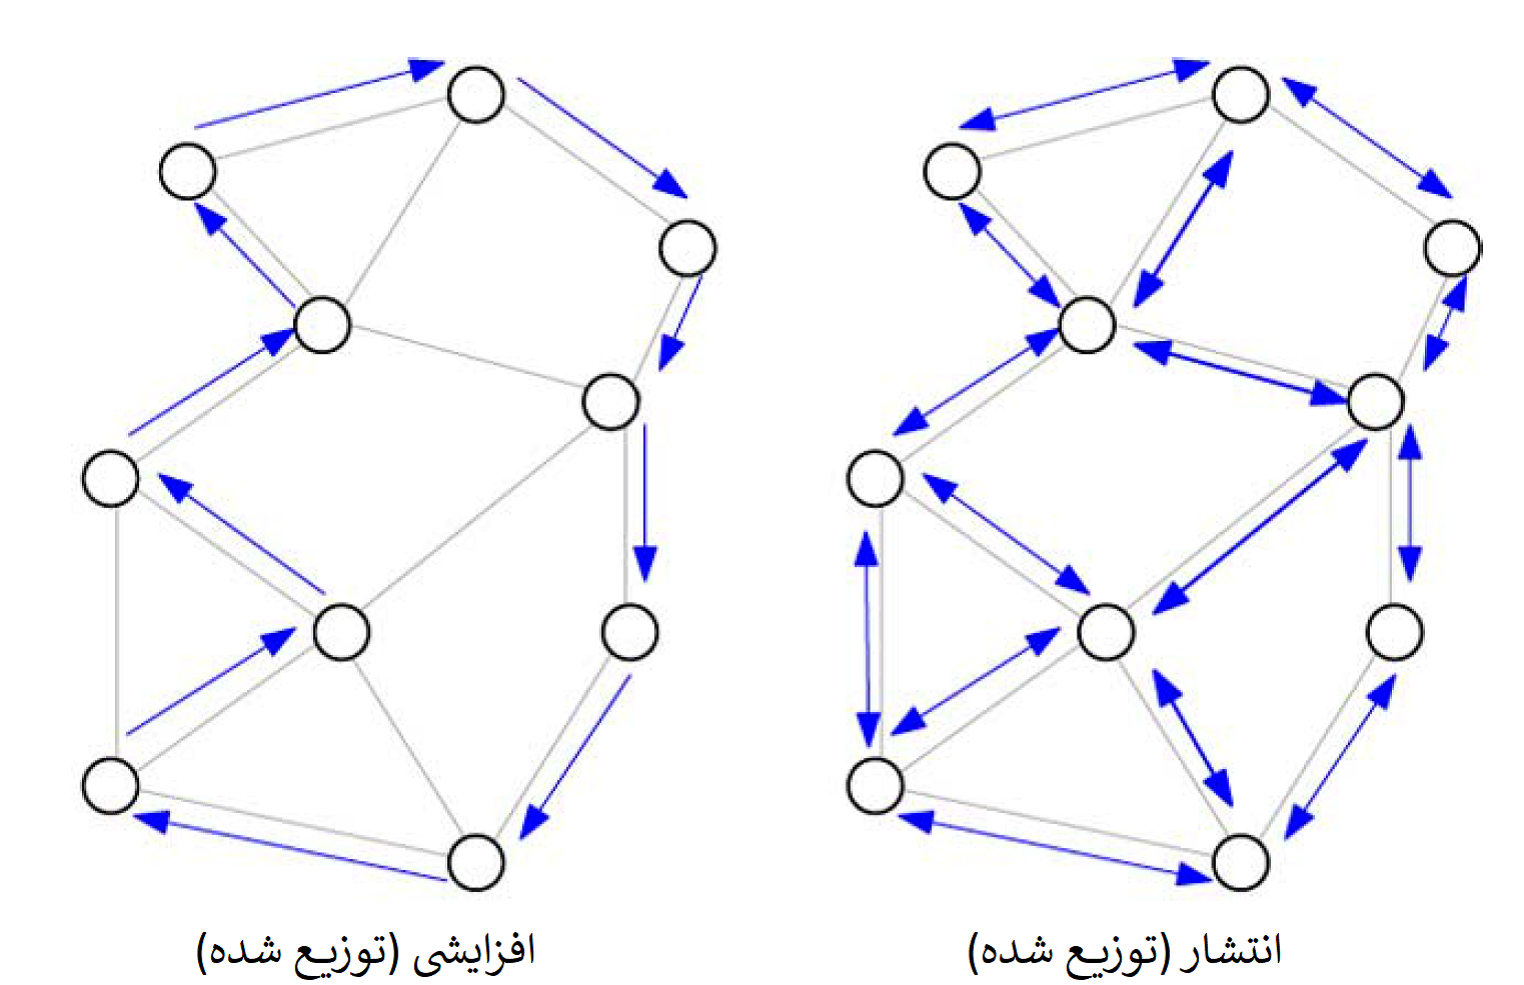
\includegraphics[scale=0.4]{Pic1.png}
		\caption{روش‌های مختلف همکاری بین گره‌ها در یک شبکه توزیع‌شده \cite{Sayed2014} }
		\label{p1}
	\end{center}
\end{figure}

فرض کنید یک شبکه متصل غیرجهت‌‌دار $G(V,E) $ مفروض است که $V$ مجموعه گره‌های شبکه و $E$ مجموعه یال‌های شبکه می‌باشد. گره‌ها در این شبکه تطبیقی با همکاری همدیگر اقدام به حل مساله بهینه‌سازی زیر می‌نمایند:


\begin{equation}\label{e1}
	w_o=\argminA_{w} J^{glob}(w)
\end{equation}

\begin{equation}\label{e2}
	J^{glob}(w)=\frac{1}{N}\sum_{k=1}^{N} J_k(w)
\end{equation}

که $N$ تعداد گره‌های شبکه، $M$ اندازه بردار وزن یا مرتبه فیلتر و $J_k (w)$ تابع زیان محدب و مشتق‌پذیر در گره $k$ام است. $J^{glob} (w)$  تابع زیان سراسری شبکه است که گره‌ها با همکاری همدیگر، پارامتر سراسری $w_o$ را جستجو می‌نمایند. شکل\ref{p2} یک شبکه تطبیقی توزیع‌شده با 12 گره را نشان می‌دهد که هر گره تابع زیان اختصاصی $J_k (w)$ را دارد و تنها با همسایگان خود تبادل اطلاعات انجام می‌دهد. مجموعه $N_k=\{k,l,8,9,N\}$ همسایگان گره \lr{k} را نشان‌می‌دهد که گره $k$ فقط با آنها تبادل داده و همکاری دارد  \cite{Sayed2007}.

\begin{figure}[t!]
	\begin{center}
		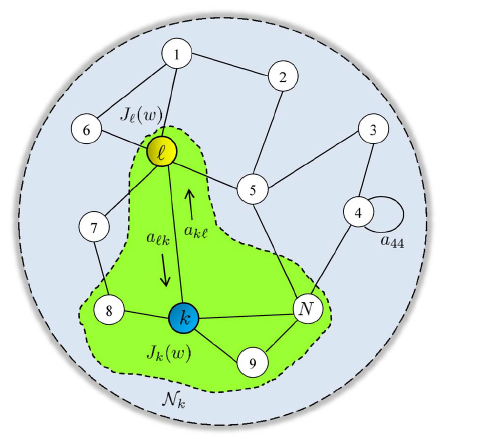
\includegraphics[scale=0.6]{Pic2.png}
		\caption{یک شبکه تطبیقی توزیع‌شده با 12 گره \cite{Sayed2007}}
		\label{p2}
	\end{center}
\end{figure}


اکثر کارهای ارائه‌شده در زمینه برآورد پارامتر از طریق شبکه‌های توزیع‌شده به صورت یک مساله کمینه‌سازی اجماع توابع هزینه هر گره مطرح می‌شوند. گره‌ها با توابع زیان مجزا اما هم مدل در جستجوی یک هدف هستند و نیاز به همگرا شدن به سمت یک پارامتر مشترک دارند. این مسائل تک‌وظیفه‌ای\footnote{\lr{Single Task}} نامیده می‌شوند. دسته دیگر مسائل که هر گره یا گروهی از گره‌ها به دنبال هدف‌هایی مجزا می‌باشند، چند وظیفه‌ای نامیده می‌شوند. 

با فرض داشتن یک شبکه متصل با $N$ گره $(k=1,2,…,N)$، هر گره شبکه در زمان $i$ یک مقدار اسکالر $d_k(i)$ به عنوان سیگنال مطلوب و یک بردار ورودی $u_k (i)\in R^M$ با ماتریس کوواریانس $R_{u,k}=E\{u_k (i),u_k^T (i)\}$ دریافت می‌کند. ورودی‌های هر گره یا مدل داده به صورت زیر با یک رگرسیون خطی مدل می‌شوند:

\begin{equation}\label{e6}
	d_k(i)=u_k^T(i)w^o+\nu_k(i)\qquad i>=0, k=1,2,...,N
\end{equation}

که $w^o$ بردار پارامترها به طول $M$ است و گره‌ها در طی فرآیند یادگیری به دنبال برآورد آن می‌باشند. $z_k (i) $ یک نویز اندازه‌گیری با میانگین صفر و واریانس $\sigma_\nu^2$ می‌باشد. تابع زیان میانگین مربعات خطا (\lr{MSE}) برای هر گره به صورت زیر تعریف می‌شود: 

\begin{equation}\label{e7}
	j_k(w)=E(d_k(i)-u_k^T(i)w)^2
\end{equation}

گره‌ها به دنبال برآورد بردار پارامتر مشترک $w^o$ با استفاده از تابع زیان $J_k (w)$ در شبکه تطبیقی تک‌وظیفه‌ای هستند. شکل \ref{p6} یک شبکه تطبیقی تک وظیفه‌ای را نشان می‌دهد. از آنجایی که تابع زیان در رابطه \ref{e7} یک تابع اکیدا محدب \footnote{\lr{Strongly convex}} است، پس دارای یک مینیمم سراسری $w_k^o$ است. در نتیجه پارامتر $w^o$ در رابطه \ref{e6} همان $w_k^o$ می‌باشد.

\begin{figure}
	\begin{center}
		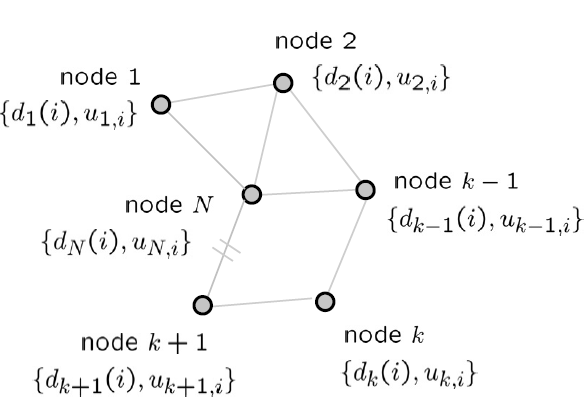
\includegraphics[scale=0.5]{Pic6.png}
		\caption{شبکه تطبیقی تک‌وظیفه‌ای \cite{Bo2010}}
		\label{p6}
	\end{center}
\end{figure}


\section{مدل‌های محاسباتی پردازش موازی و توزیع‌شده}

امروزه با افزایش حجم داده‌های پردازشی و محاسبات سنگین در بسیاری از کاربردها، چالش‌های مهمی در فرآیند یادگیری الگوریتم‌ها مطرح شده است. در یک شبکه تطبیقی توزیع‌شده، اگر عملیات محاسباتی در فرآیند تخمین برای گره‌ها سنگین باشد و یا داد‌های ورودی ذاتاً توزیع‌شده و برای ذخیره در یک گره بسیار بزرگ باشند، مهمترین چالش در این نوع یادگیری، موازی‌سازی فرآیند آموزش و ایجاد یک مدل منسجم در کل شبکه است. یادگیری موازی بهتر است تحت یک مدل یا چارچوب محاسباتی موازی پیاده‌سازی و اجرا شود. در سال‌های اخیر به منظور پردازش‌های موازی و پیاده‌سازی الگوریتم‌های توزیع‌شده مدل‌ها و چارچوب‌های محاسباتی زیادی با ویژگی‌ها و کاربردهای مختلف مورد مطالعه قرار گرفته است. از جمله این مدل‌های محاسباتی می‌توان به \lr{PRAM}، \lr{LogP}، \lr{BSP} و چارچوب \lr{MapReduce} اشاره کرد. 
\subsection{مدل محاسباتی \lr{PRAM}}
مدل محاسباتی \lr{PRAM} (ماشین موازی با دستیابی تصادفی) \cite{Ja1992} یک مدل حافظه اشتراکی است که در آن ارتباط بین پردازنده‌ها از طریق حافظه اشتراکی انجام می‌شود. در صورتی که پردازنده $i$ بخواهد داده‌ای را به پردازنده $j$ ارسال کند، در دو مرحله انجام می‌شود. ابتدا پردازنده $i$ داده را در حافظه مشترک در یک محل شناخته شده برای پردازنده $j$ می‌نویسد و پردازنده $j$ داده را از محل مورد نظر می‌خواند. شکل \ref{P32} مدل محاسباتی \lr{PRAM} را نشان می‌دهد. کامپیوترهای مبتنی بر مدل \lr{PRAM} بر اساس نحوه دسترسی هم‌زمان به یک مکان یکسان به چهار دسته \lr{EREW}، \lr{CREW}، \lr{ERCW} و \lr{CRCW} تقسیم می‌شوند. عمدتاً به این دلیل که هزینه ارتباطات بیشتر از هزینه محاسبات بوده و تعداد پردازنده‌ها محدود می‌باشد، این مدل برای پیاده‌سازی همه‌منظوره در سخت‌افزار مناسب نیست و همچنین منجر به یک مدل برنامه‌نویسی نمی‌شود.
\begin{figure}[t!]
	\begin{center}
		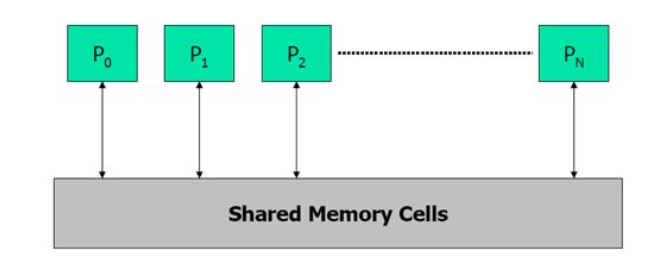
\includegraphics[scale=0.7]{Pram.JPG}
		\caption{مدل محاسباتی\lr{PRAM}\cite{Ja1992} }
		\label{P32}
	\end{center}
\end{figure}

\subsection{مدل محاسباتی \lr{LogP}}
ماشین انتزاعی مدل محاسباتی \lr{LogP} \cite{Logp} شامل تعداد زیادی  پردازنده با حافظه توزیع‌شده است. پردازنده‌ها از طریق یک شبکه ارتباطی انتزاعی به هم متصل می شوند که امکان ارتباط نقطه به نقطه را فراهم می‌کند و به صورت جفتی همگام و به طور کلی غیرهمگام هستند. این مدل با چهار پارامتر زیر توصیف می‌شود:
\begin{itemize}
	\item
	\lr{L}، تأخیر رسانه ارتباطی
	\item
	\lr{o}، هزینه ارسال و دریافت پیام
	\item
	\lr{g}، فاصله مورد نیاز بین دو عملیات ارسال/دریافت. تعبیر رایج تر از این کمیت، معکوس پهنای باند یک کانال ارتباطی پردازنده-پردازنده است
	\item
	\lr{P}، تعداد پردازنده‌ها
\end{itemize}
هر عملیات محلی بر روی هر دستگاه زمان یکسانی را می‌طلبد.  این زمان چرخه پردازنده نامیده می‌شود. شکل \ref{P33} مدل محاسباتی \lr{LogP} و پارامترهای مهم این مدل را به تصویر کشیده است. ارتباطات در این مدل یک نمای محلی بر اساس عملکرد هر جفت پردازنده دارد. 
\begin{figure}[t!]
	\begin{center}
		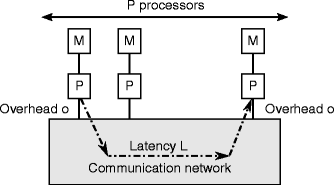
\includegraphics[scale=0.7]{logp.png}
		\caption{مدل محاسباتی\lr{LogP} \cite{LogP2011}}
		\label{P33}
	\end{center}
\end{figure}
\subsection{چارچوب محاسباتی \lr{MapReduce}}
یکی از روش‌های پردازش مجموعه داده‌های عظیم، چارچوب نگاشت-کاهش یا \lr{MapReduce} نام دارد و توجه محققان زیادی را تا کنون به خود جلب کرده است. این چارچوب توسط گوگل\cite{De2008} توسعه یافته و به طور گسترده مورد استفاده قرار گرفته است. اجرای متن باز آن \lr{Hadoop} \cite{Apache58} در حال حاضر توسط بیش از 100 شرکت در سراسر جهان از جمله \lr{eBay}، \lr{IBM}، \lr{Yahoo!}، \lr{Facebook} و \lr{Twitter} و تعدادی از دانشگاه‌ها استفاده می‌شود \cite{Apache59}. برخی از شرکت‌ها مانند آمازون و مایکروسافت به کاربران خود اجازه می‌دهند تا برنامه‌های نگاشت-کاهش را روی ابر خود اجرا کنند \cite{Apache60,Apache61}. الگوریتم‌های نگاشت-کاهش برای حل تعدادی از مسائل غیر پیش پا افتاده در زمینه‌های مختلف از جمله پردازش داده‌ها، داده‌کاوی و تجزیه و تحلیل گراف استفاده شده است.

\lr{Dean}  و همکارش در سال 2004  \cite{De2008} چارچوب محاسبات موازی نگاشت-کاهش را معرفی کردند. ایده اصلی این چهارچوب از زبان‌های مانند \lr{Lisp} گرفته شده است. عمل نگاشت یک تابع و یک دنباله را به عنوان ورودی می‌گیرد و این تابع را بر روی تمام عناصر موجود در دنباله اعمال می‌کند. عمل کاهش، با توجه به یک توالی از مقادیر و یک تابع دودویی، از این تابع برای ترکیب عناصر دنباله‌ در یک مقدار خروجی واحد استفاده می‌کند. دو عمل نگاشت و کاهش در تعدادی دور یا \lr{Round} اجرا می‌شوند و اساس چهارچوب نگاشت-کاهش را تشکیل می‌دهند که در اصل برای اجرا بر روی خوشه‌های بزرگی از ماشین‌های ارزان قیمت طراحی شده‌اند. هر ماشینی یک پردازنده، یک حافظه اولیه سریع و یک حافظه ثانویه کندتر دارد و از طریق یک شبکه زیربنایی به بقیه خوشه متصل است. حافظه ثانویه بخشی از حافظه اشتراکی سراسری است  که هر ماشین تنها در حین همگام‌سازی اجازه دسترسی به حافظه ثانویه ماشین‌های دیگر را دارد. 

داده‌ها در یک الگوریتم نگاشت-کاهش به صورت زوج‌های کلید-مقدار مشخص می‌شوند. همان طور که در شکل\ref{p3} نشان داده شده است، یک الگوریتم نگاشت-کاهش شامل تعدادی دور است که هر دور یک فاز نگاشت و یک فاز کاهش دارد. هر فاز از یک ورودی، یک محاسبات و یک مرحله خروجی تشکیل شده است که خروجی هر فاز به عنوان ورودی فاز بعدی استفاده می‌شود. هنگامی که یک فاز تمام می‌شود، یعنی زمانی که هر ماشین داده‌های خروجی خود را در حافظه اشتراکی می‌نویسد، داده‌ها همگام می‌شوند و هر ماشین اجازه دارد داده‌های نوشته شده در فاز قبلی را بخواند. ماشین‌ها تنها مجاز به برقراری ارتباط با پردازنده اصلی می‌باشند. حافظه اولیه محلی هر ماشین قبل از هر همگام‌سازی به طور کامل پاک می‌شود. در چارچوب نگاشت-کاهش موازی‌سازی از طریق داشتن ماشین‌های مختلف که عملکردهای یکسانی را روی داده‌های مختلف انجام می‌دهند، به دست می‌آید. 
\begin{figure}[t!]
	\begin{center}
		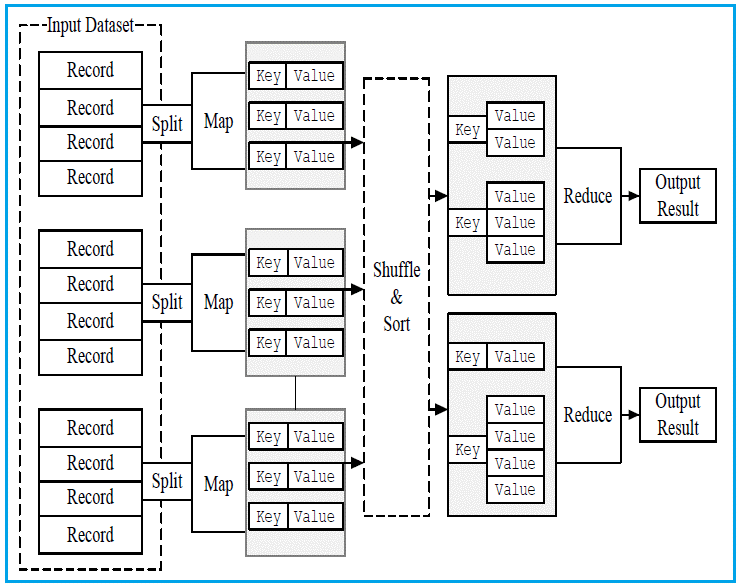
\includegraphics[scale=0.6]{Pic3.png}
		\caption{یک دور در چارچوب نگاشت-کاهش شامل فازهای \lr{Map} و \lr{Reduce} \cite{De2008}}
		\label{p3}
	\end{center}
\end{figure}

\subsection{مدل محاسباتی \lr{BSP}}
مدل محاسباتی \lr{BSP} (موازی‌سازی با همگامی مانعی) \cite{Va1990} تعمیمی از مدل محاسباتی \lr{PRAM} است که توسط پروفسور \lr{L. G. Valiant } از دانشگاه هاروارد در سال 1990 به عنوان یک مدل پل برای محاسبات موازی پیشنهاد شده است. در طی سالهای گذشته این مدل توسط پروفسور \lr{McColl} و \lr{Valiant} توسعه یافته است.  مدل محاسباتی \lr{BSP} شامل بخش‌های زیر می‌باشد:
\begin{itemize}
	\item
	مجموعه‌ای از کامپیوترها که هر یک دارای حافظه محلی می‌باشند
	\item 
	یک شبکه ارتباطی که پیام‌ها را از نقطه‌ای به نقطه دیگر انتقال می‌دهد
	\item 
	مکانیزمی که همگام‌سازی همه یا گروهی از پردازنده‌ها را انجام می‌دهد. 
\end{itemize}
برنامه‌های \lr{BSP} به صورت دنباله‌ای از ابرگام‌ها\footnote{\lr{Superstep}} نوشته می‌شوند. هر ابرگام از سه بخش اصلی تشکیل شده است: محاسبات بر روی داده‌های محلی، ارسال و دریافت پیام به منظور دسترسی به داده‌های غیرمحلی و همگام‌سازی مانعی به منظور تکمیل همه عملیات ارتباطی و از سرگیری محاسبات روی داده‌های محلی یا داده‌هایی که از طریق تبادل پیام به یک پردازنده رسیده‌اند. شکل \ref{p4} بخش‌های مختلف یک ابرگام را به تصویر کشیده است.
\begin{figure}[t!]
	\begin{center}
		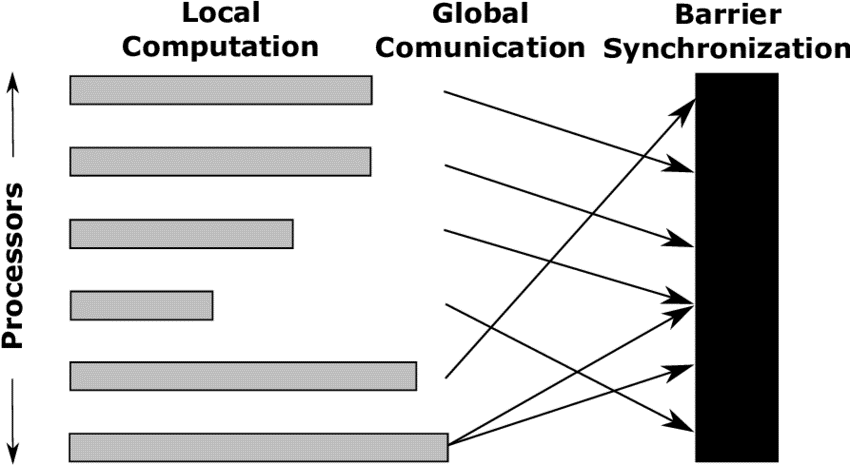
\includegraphics[scale=0.4]{Pic4.png}
		\caption{یک ابرگام در مدل محاسباتی \lr{BSP} \cite{Va1990}}
		\label{p4}
	\end{center}
\end{figure}

یکی از مزیت‌های این مدل محاسباتی این است که می‌توان با استفاده از چهار پارامتر، زمان اجرای یک رویکرد یا الگوریتم طراحی شده بر اساس آن مدل را پیش‌بینی کرد. در بخش \ref{BSP_Dec} به طور مفصل نحوه پیش‌بینی زمان اجرا شرح داده خواهد شد. 

\section{مدل محاسباتی موازی‌ مانعی یا \lr{BSP}}\label{BSP_Dec}

یک کامپیوتر \lr{BSP} شامل مجموعه‌ای از جفت پردازنده-حافظه، یک شبکه ارتباطی کلی و مکانیزمی برای همگام‌سازی مانعی کارآمد پردازنده‌ها است. یک کامپیوتر \lr{BSP} به روش زیر عمل می‌کند. محاسبات شامل دنباله‌ای از ابرگام‌های موازی است، که در آن هر ابرگام متشکل از دنباله‌ای از مراحل است، و به دنبال آن یک همگام‌سازی مانع انجام می‌شود که در آن نقطه، تمام ارتباطات داده تکمیل می‌شوند. در طول یک ابرگام، هر پردازنده می‌تواند تعدادی از مراحل محاسباتی را روی مقادیری که در شروع ابرگام در حافظه محلی‌اش ذخیره می‌شوند، انجام دهد، تعدادی پیام ارسال و دریافت کند، و درخواست‌های مختلف خواندن و نوشتن از راه دور را مدیریت کند\cite{Bisseling2020}.

کامپیوتر \lr{BSP} یک مدل حافظه دو سطحی است، یعنی هر پردازنده ماژول حافظه محلی خود را دارد. تمام حافظه‌های دیگر غیرمحلی هستند و به روشی کارآمد یکنواخت قابل دسترسی می‌باشند. منظور از کارآمدی یکنواخت این است که زمان صرف شده برای خواندن یا نوشتن یک عنصر حافظه غیرمحلی در یک جفت  پردازنده-حافظه دیگر باید مستقل از این باشد که مقدار آن در کدام ماژول حافظه فیزیکی قرار دارد. طراح الگوریتم و برنامه‌نویس نیازی ندارد تا از ساختار حافظه سلسله مراتبی و ساختار خاص شبکه ارتباطی آگاه باشد.

مدل محاسباتی \lr{BSP} هم ساختار افقی (مکانی) و هم ساختار عمودی (زمانی) دارد. ساختار افقی ناشی از همگامی است و از تعداد ثابتی از نخ‌های مجازی تشکیل شده است. در زمان اجرا هر کدام از تردها با یک پردازنده فیزیکی مرتبط هستند. ساختار عمودی از پیشرفت یک محاسبات در طول زمان ناشی می‌شود. در \lr{BSP}، این یک ترکیب متوالی از ابرگام‌های کلی است که به طور مفهومی تمام عرض معماری اجرا را اشغال می‌کند. هر ابرگام به سه مرحله تقسیم می‌شود که شامل موارد زیر می‌باشد:
\begin{itemize}
	\item محاسبات محلی در هر ترد، تنها با استفاده از مقادیر ذخیره شده در حافظه محلی هر پردازنده.
	\item اقدامات ارتباطی، به عنوان مثال. ارسال و دریافت، در میان تردها، شامل انتقال داده‌ها بین پردازنده‌ها
	\item همگام‌سازی مانع، که منتظر می‌ماند تا تمام اقدامات ارتباطی کامل شوند، و سپس داده‌های منتقل شده را در حافظه‌های محلی پردازنده‌های مقصد در دسترس قرار می‌دهد.
\end{itemize}
همجنین می‌توان با استفاده از چهار پارامتر، زمان اجرای یک رویکرد یا الگوریتم طراحی شده بر اساس مدل محاسباتی \lr{BSP} را پیش‌بینی کرد. این چهار پارامتر به صورت زیر تعریف می‌شوند:
\begin{itemize}
	\item $l$: تاخیر شبکه و به معنی کمترین تعداد گام‌های زمانی ممکن بین عملیات همگام‌سازی است
	\item  $p$: تعداد پردازنده‌ها
	\item $s$: سرعت پردازنده‌ها
	\item $g$: نرخ راندمان ارتباطات و به عبارت دیگر تعداد کل عملیات محلی انجام شده به وسیله همه پردازنده‌ها در یک ثانیه تقسیم‌بر تعداد کل کلمات انتقال داده شده توسط شبکه ارتباطی در یک ثانیه است
\end{itemize}

پارامترهای $l=l(p)$ و $g=g(p)$ تابعی از پارامتر $p$ هستند. برای بیان مفهوم این پارامترها باید \lr{h-relation } معرفی شود. \lr{h-relation } یک الگوی ارتباطی سراسری است به این معنا که هر پردازنده می‌تواند حداکثر $h$ واحد داده بفرستد یا دریافت کند. واحدها می‌توانند کلمات یا پیام‌ها باشند. هزینه انجام یک \lr{h-relation } به صورت \lr{gh} تعریف شده است. تعریف هزینه به این صورت بیان می‌شود که فرقی بین فرستادن \lr{m} پیام شامل یک واحد داده یا یک پیام شامل \lr{m } واحد داده وجود ندارد. هزینه هر دو حالت \lr{mgh} است. هزینه یک برنامه \lr{BSP} می‌تواند با استفاده از پارامترهای توصیف‌ شده و برخی اطلاعات اضافی پیش‌بینی شود. هزینه یک ابرگام در محاسبات موازی می‌تواند به صورت زیر بیان شود:

\begin{equation}\label{e4}
	C_s=max{\{w_i\}}+max{\{h_i g\}}+l
\end{equation}

که $C_s$ هزینه ابرگام $s$ و $w_i$ زمان محاسبات پردازنده $i$ در ابرگام $s$ است. $l$ تاخیر شبکه است. پارامتر $h_i$ تعداد واحدهای داده که پردازنده $i$ در طول ابرگام می‌فرستد یا دریافت می‌کند. پارامترهای $w$، $g$ و $l$ باید برحسب سرعت پردازنده بیان شوند. مقادیر $w_i$ و $h_i $ می‌توانند با اندازه‌گیری زمان استفاده شده و تعداد بایت‌های فرستاده شده محاسبه شوند. هزینه‌های یک برنامه \lr{BSP} در $S$ ابرگام شامل $W=\sum_{s=1}^{S}w_s$ و $H=\sum_{s=1}^{S}h_s$ است که در مجموع به صورت زیر بیان می‌شود:
\begin{equation}\label{e5}
	C=W+H.g+S.l
\end{equation}

هزینه یک ابرگام به کندترین پردازنده، بیشترین میزان داده‌ای که یک پردازنده می‌فرستد یا دریافت می‌کند و هزینه همگام‌سازی بستگی دارد. هزینه یک برنامه \lr{BSP } برابر با مجموع هزینه همه ابرگام‌ها در برنامه است \cite{Bisseling2020}. با توجه به فرمول فوق مشخص می‌شود که فاکتورهای مهم در ایجاد و طراحی برنامه‌های \lr{BSP} عبارتند از:
\begin{itemize}
	\item 
	محاسبات در هر ابرگام باید بین پردازنده‌ها متوازن باشد
	\item
	ارتباطات بین همه پردازنده‌ها باید متوازن باشد تا از اختلافات بزرگ $h_i$ اجتناب شود
	\item 
	به دلیل هزینه بالای همگام‌سازی، تعداد ابرگام‌ها باید به حداقل برسد
\end{itemize}

الگوریتم‌ها یا برنامه‌های بالانس‌شده از طریق تقسیم بار محاسباتی و ارتباطی به طور مساوی بین پردازنده‌های در دسترس حاصل خواهند شد. پارامترهای $l$ و $g$ در بین پیاده‌سازی‌های سیستم متغیر هستند. در مقایسه مدل‌های محاسباتی موازی، می‌توان گفت که در مدل \lr{BSP} محاسبات در یک ابرگام می‌توانند زمان‌های متفاوتی داشته باشند و همچنین هزینه‌های ارتباط و همگام‌سازی به صراحت در نظر گرفته شده است، در حالی‌که در مدل \lr{PRAM} این چنین نیست. مدل \lr{PRAM} منجر به یک مدل برنامه‌نویسی نمی‌شود، اما مدل \lr{BSP} دارای یک مدل برنامه‌نویسی است و هیچ محدودیتی بر روی تعداد پردازنده‌ها ندارد. ارتباط در مدل \lr{LogP} یک نمای محلی بر اساس عملکرد هر جفت پردازنده دارد، در حالی‌که ارتباط در مدل \lr{BSP} یک نمای کلی بر اساس عملکرد برای کل برنامه دارد. 

\subsection{تاریخچه مدل محاسباتی \lr{BSP}}
مدل محاسباتی \lr{BSP} در طول دهه 1980 توسط پروفسور \lr{L. Valiant} از دانشگاه هاروارد  توسعه یافته است که مقاله آن در سال 1990  منتشر شد. در بازه 1990 تا 1992، \lr{L. Valiant} و \lr{B. McColl} از دانشگاه آکسفورد در پرینستون و هاروارد روی ایده‌هایی برای مدل برنامه‌نویسی \lr{BSP} حافظه توزیع‌شده کار کردند. در بازه 1992 تا 1997، پروفسور \lr{McColl} یک تیم تحقیقاتی بزرگ را در آکسفورد رهبری کرد که کتابخانه‌ها، زبان‌ها و ابزارهای مختلف برنامه‌نویسی \lr{BSP}، و همچنین الگوریتم‌های موازی متعدد \lr{BSP}، از جمله بسیاری از نمونه‌های اولیه از الگوریتم‌های موازی اجتناب از ارتباط با کارایی بالا و الگوریتم‌های موازی بازگشتی «جاودانه» را توسعه دادند که به بهترین عملکرد ممکن و مبادلات پارامتریک بهینه دست یافتند.

در سال 1996، \lr{McColl} گروهی از آکسفورد، هاروارد، فلوریدا، پرینستون، آزمایشگاه‌های بل، کلمبیا و اوترخت را رهبری کرد که استاندارد \lr{BSPlib} را برای برنامه‌نویسی \lr{BSP} توسعه و منتشر کردند. در دهه 2000، \lr{Valiant} توسعه‌ای برای مدل \lr{BSP} ایجاد کرد که منجر به انتشار مدل \lr{Multi-BSP} در سال 2011 شد \cite{MultiBSP}. 

در سال 2018، پروفسور \lr{McColl} یک تعمیم جدیدی از مدل \lr{BSP} ایجاد کرد که تحمل خطا را برای محاسبات موازی در مقیاس بزرگ در هوش مصنوعی، تجزیه و تحلیل و محاسبات ابری با عملکرد بالا ارائه کرد \cite{BridgingMcColl}.

در سال 2010، گوگل پس از سال‌ها تجربه محدودیت‌های \lr{MapReduce} متوجه شد که به یک مدل جدید برای پشتیبانی از مسائل تحلیلی و محاسباتی گراف‌ها در مقیاس بزرگ نیاز دارند. آنها به سرعت متوجه شدند که با استفاده از مدل \lr{BSP} به روشی داده-محور می‌توانند به اهداف بلندپروازانه‌ای که از نظر مقیاس‌پذیری و عملکرد داشتند، دست یابند. نتیجه سیستم جدید گوگل به نام \lr{Pregel} \cite{Pregle2010} بود که با عبارت جدید "همانند یک راس فکر کن"\footnote{\lr{Think Like a Vertex}} همراه بود \cite{McColl2021}.

در ادامه کار گوگل بر روی \lr{Pregel}، یک سیستم \lr{BSP} منبع-باز داده-محور برای محاسبات گراف به نام \lr{Apache Giraph} توسعه یافت و از آن زمان به بعد چندین سیستم‌ها این چنینی ظاهر شدند. امروزه، \lr{BSP} داده-محور به روشی استاندارد برای انجام محاسبات گراف در مقیاس بزرگ در پایگاه داده‌ها و سایر سیستم‌های تحلیلی، تبدیل شده است.

همانطور که ذکر شد، ایده اصلی پشت سیستم‌های \lr{BSP} داده-محور مانند \lr{Pregel} این است که "مثل راس فکر کنید". این بدان معنی است که ساختار داده، برای مثال، یک گراف با یک میلیارد راس باید به یک محاسبات موازی مجازی نگاشت شود که در آن راس‌ها به محاسبات محلی و یال‌ها به ارتباطات تبدیل می‌شوند. همانند تمام سیستم‌های \lr{BSP}، محاسبات در قالب مجموعه‌ای از دورها یا ابرگام‌ها انجام می‌شود. همانطور که در شکل \ref{BSPDataCenter} نشان داده شده است، در هر دور، هر رأس محاسبات محلی را انجام می‌دهد، پیام‌هایی را به همسایگان خود در گراف ارسال می‌کند و پیام‌هایی را از همسایگان خود دریافت می‌کند. این محاسبات تکراری تا زمانی‌که برخی از شرایط خاتمه برآورد شوند، ادامه می‌یابند \cite{McColl2021}.
\begin{figure}[h]
	\begin{center}
		\includegraphics[scale=0.8]{BSP3step.PNG}
		\caption{\lr{BSP} داده-محور \cite{McColl2021}}
		\label{BSPDataCenter}
	\end{center}
\end{figure} 

در سیستم‌های مبتنی بر \lr{BSP}، ماهیت ابرگام‌ها تضمین می‌کند که هیچ مشکل هم‌زمانی از جمله شرایط مسابقه\footnote{\lr{race conditions}} یا بن‌بست\footnote{\lr{deadlock}} رخ نخواهد داد. البته میزان ریزدانگی موازی بودن مجازی یا منطقی در چنین محاسباتی می‌تواند بسیار زیاد در حد یک میلیارد یا یک تریلیون باشد. از سوی دیگر، ماشین‌های موازی کاربردی معمولاً تنها چند صد یا چند هزار هسته خواهند داشت. بنابراین، همانطور که قبلا ذکر شد، این محاسبات مجازی مقیاس بزرگ را می‌توان به راحتی بر روی یک ماشین موازی فیزیکی در مقیاس بسیار کوچکتر به روشی ساده و سرراست  که ساختار محلی گراف را برای بهینه‌سازی ارتباطات در نظر می‌گیرد، نگاشت کرد.

سیستم‌های \lr{BSP} داده-محور در سال‌های اخیر به طور گسترده توسط بسیاری از شرکت‌ها در سراسر جهان برای محاسبات کاربردی بر روی گراف‌هایی با میلیاردها راس و تریلیون‌ها یال استفاده شده است. علاوه‌بر ارائه مقیاس‌پذیری زیاد و عملکرد بسیار بالا، یادگیری و استفاده از این مدل نیز بسیار آسان است. برای مثال، الگوریتم رتبه‌بندی صفحات \footnote{\lr{PageRank Algorithm}} گوگل که نقش اساسی در روش‌های جستجوی آن‌ها دارد را می‌توان تنها در 15 تا 20 خط کد توصیف کرد، زیرا این الگوریتم را می‌توان در \lr{BSP} داده-محور به‌ صورت محاسبات تکراری ساده زیر فرمول‌بندی کرد:
\begin{enumerate}
	\item خواندن رتبه همسایه‌ها
	\item به‌روزرسانی رتبه محلی
	\item ارسال رتبه جدید به همسایه‌ها
\end{enumerate}

شرکت پایگاه‌داده \lr{TigerGraph} اعلام کرد که پایگاه داده گراف \lr{BSP} داده-محور آن‌ها اکنون سریع‌ترین پایگاه داده گراف تراکنشی در جهان است که حجم عظیمی از تجارت الکترونیک و تراکنش‌های مالی را مدیریت می‌کند. اگرچه در پاراگراف‌های اخیر بیشتر بر مبحث تجزیه و تحلیل گراف با مدل \lr{BSP} داده-محور تاکید شده است، اما در بسیاری از دسته‌های دیگر محاسبات موازی نیز این مدل قابل استفاده است. به عنوان مثال، می‌توان از آن در محاسبات علمی و مهندسی مانند محاسبات شابلون\footnote{\lr{Stencil Computations}}، مسائل \lr{n}-جسم\footnote{\lr{n-body Problems}}، اجزای محدود و مدل‌سازی مدار و همچنین در یادگیری ماشین و سایر زمینه‌های هوش مصنوعی استفاده کرد.


\subsection{برتری‌های مدل محاسباتی \lr{BSP}}
\textbf{همه‌منظوره بودن}

اساس روش \lr{BSP} برای برنامه‌نویسی موازی مفهوم ابرگام است که در آن ارتباطات و همگام‌سازی به طور کامل از هم جدا شده‌اند. یک برنامه \lr{BSP} صرفا برنامه‌ای متشکل از تعدادی فاز است و ارتباطات لازم بین فازها انجام می‌شود. این روش برای برنامه‌نویسی موازی بر روی تمام انواع معماری‌های موازی و الگوریتم‌های موازی قابل اجرا است. این روش یک چارچوب منسجم و بسیار کلی  را برای توسعه نرم‌افزارهای موازی قابل حمل برای معماری‌های موازی مقیاس‌پذیر فراهم می‌کند.

\textbf{سادگی}

برنامه‌های \lr{BSP} تقریبا مشابه برنامه‌های متوالی هستند. تنها اطلاعات اضافی اندکی برای توصیف استفاده از موازی‌سازی باید ارائه شود. 

\textbf{اشکال‌زدایی آسان و بدون بن‌بست}

در حالی‌که ارتباطات و همگام‌سازی در برنامه \lr{BSP} جدا شده‌اند، برنامه‌نویس دیگر لازم نیست نگران مشکلاتی از جمله بن‌بست که می‌تواند با ارسال پیام همگام‌سازی رخ دهد، باشد. به دلیل این جداسازی، اشکال‌زدایی یک برنامه \lr{BSP} بسیار آسان‌تر انجام می‌شود. مانع همگام‌سازی قرار گرفته در انتهای هر ابرگام یک نقطه شکست مناسبی را فراهم می‌کند که در آن حالت کلی محاسبات موازی به خوبی تعریف شده است و می‌تواند مورد بررسی قرار گیرد. بنابراین اشکال‌زدایی و استدلال در مورد درستی یک برنامه \lr{BSP} دشوارتر از یک برنامه متوالی نیست. 

\textbf{قابل حمل بودن و مستقل از معماری هدف}

برخلاف مدل‌های برنامه‌نویسی موازی، \lr{BSP} به صورت یک مدل مستقل از معماری طراحی شده است. بنابراین زمانی‌که برنامه‌ها از یک معماری به معماری دیگری منتقل می‌شوند، بدون نیاز به هیچگونه تغییری اجرا می‌شوند. این امر کاوش فضای طراحی را ممکن می‌سازد، زیرا تأثیر یک تصمیم بر عملکرد به راحتی قابل تعیین است.

\textbf{قابل تجزیه و تحلیل بودن}

مدل هزینه \lr{BSP} روشن می‌کند که چه استراتژی‌هایی باید برای نوشتن برنامه‌های \lr{BSP} کارآمد اتخاذ شود. با توجه به اینکه پارامتر $W$ حداکثر زمان محاسباتی را نشان می‌دهد، باید محاسبات بین رشته‌ها را متعادل و به حداقل رساند. از آنجایی‌که پارامتر $h$ حداکثر داده مبادله شده است، باید ارتباطات بین رشته‌ها را متعادل و به حداقل رساند. تعداد ابرگام‌ها باید به حداقل برسد، زیرا این مورد تعداد دفعاتی که پارامتر $L$ در هزینه نهایی ظاهر می‌شود را تعیین می‌کند. همچنین مدل هزینه چگونگی پیش‌بینی کارآیی روی یک معماری هدف خاص را نشان می‌دهد. مقادیر پارامترهای $W$ و $h$ برای هر ابرگام، و تعداد ابرگام‌ها می‌توانند با بررسی کد برنامه تعیین شوند. با درج مقادیر پارامترهای $p$، $g$ و $L$ می‌توان زمان اجرا را قبل از اجرای برنامه مشخص کرد. 

\textbf{استفاده آسان از نقطه شکست برای انعطاف‌پذیری}

این مورد اشاره دارد به این واقعیت که به راحتی می‌توان یک حالت کاملاً تعریف‌شده را در هر مانع ثبت کرد و یا به عبارت دیگر، یک راه ساده برای انجام بازرسی و بازیابی خرابی‌های سخت‌افزاری است. در مقابل، بررسی وضعیت محاسبات موازی بسیار دشوار است. در مدل محاسباتی \lr{BSP} معنای ابرگام نه تنها امکان مقابله با خرابی‌های سخت‌افزاری را فراهم می‌کند، بلکه به طور مؤثری می‌توان تأخیرهای طولانی را مدیریت کرد، که این خود یک مساله بسیار چالش‌برانگیز است.

\textbf{ارتباطات را می‌توان برای تبادل کلی بهینه کرد}

در محاسبات موازی مقیاس بزرگ، تقریباً همیشه این اتفاق می‌افتد که موازی‌سازی در نرم‌افزار بسیار بیشتر از موازی‌سازی در سخت‌افزار است. این یک نتیجه ساده از قدرت سخت‌افزار محاسباتی مدرن است. در مثالی که یک الگوریتم گراف دارای یک تریلیون کار فرعی موازی است، این وظایف فرعی بر روی یک ماشین فیزیکی که درجه موازی بسیار کمتری دارد، نگاشت می‌شوند. به عنوان مثال، ممکن است روی 200 ماشین 16 هسته‌ای نگاشت شود، در این صورت هر هسته حدود 300 میلیون کار فرعی موازی کوچک را انجام می‌دهد. همان پدیده سستی موازی‌سازی در هر حوزه‌ای از محاسبات موازی در مقیاس بزرگ از جمله محاسبات ماتریس پراکنده، یادگیری ماشین، مدل سازی، بهینه‌سازی و غیره رخ می‌دهد. 

یکی از پیامدهای اصلی سستی موازی‌سازی این است که معمولاً در هر محاسبات موازی در مقیاس بزرگ، هر پردازنده در حین انجام محاسبات با هر پردازنده دیگری ارتباط برقرار می‌کند. بنابراین، برای دستیابی به اوج عملکرد، باید سیستم‌های نرم‌افزاری موازی را طراحی کنیم که برای این الگوی کلی ارتباطات بهینه‌سازی شده باشند و در آن هر پردازنده در حال ارسال به سایرین است و از سایرین دریافت می‌کند. این الگوی ارتباطی، تبادل کل نامیده می‌شود. سیستم‌های نرم‌افزار \lr{BSP} برای تبادل کلی بهینه‌سازی شده‌اند، نه برای ارتباطات زوجی منفرد، مانند \lr{MPI} و سایر سیستم‌های ارسال پیام غیرهمگام یا همگام. زمانی که پردازنده‌ها نیاز به ارسال و دریافت میلیون‌ها مقدار به/از هر پردازنده دیگر در یک دور محاسبات موازی دارند، این امر باعث بهبود قابل توجهی در کارایی و عملکرد می‌شود.

\textbf{ارتباطات می‌تواند غیر مسدودکننده و یک طرفه باشند}

سیستم‌های تبادل پیام همانند \lr{MPI} براساس ارتباطات همگام بین جفت پردازنده‌ها هستند. برای اینکه پردازنده \lr{A} بتواند حتی یک مقدار را به پردازنده \lr{B} ارائه دهد، باید با \lr{B} همگام شود و سپس مقدار را به \lr{B} ارسال کند. این کار از نظر زمانی بسیار پرهزینه است، به خصوص در شرایطی که تعداد زیادی ارتباطات ریز دانه‌ای  وجود دارد که باید اتفاق بیفتد.

در طراحی مدل نرم‌افزار \lr{BSP} و در تعریف استاندارد \lr{BSPlib}، با معرفی ارتباطات یک طرفه بدون کپی غیرمسدودکننده به عنوان مدل پیش فرض ارتباطات، این مساله حل شده است. این به دلیل ساختار ابرگامی محاسبات \lr{BSP}، با مدل همگام‌سازی مانعی آن است. تغییر از ارتباطات آهسته دو طرفه \lr{MPI} به ارتباطات یک طرفه بدون کپی \lr{BSP} منجر به بهبودهای عمده در کارایی و عملکرد مسائل به ویژه برای محاسبات موازی مدرن ریزدانه مانند محاسبات ماتریس پراکنده، جابجایی نمودار و یادگیری ماشین شده است.

در \lr{BSP}، ارتباط داده‌ها را می‌توان با استفاده از \lr{RDMA} \footnote{\lr{Remote Direct Memory Access}} که هم از نظر بازده بالا و هم از نظر تأخیر بسیار کم است، پیاده‌سازی کرد. \lr{RDMA} به سبک \lr{BSP} اکنون مستقیماً در شبکه‌های ارتباطی مانند \lr{InfiniBand} پشتیبانی می‌شود. برخی از نسخه‌های جدیدتر \lr{MPI} موارد اولیه را برای ارتباطات یک طرفه اضافه کرده اند، اگرچه برای استفاده موثر از آنها نیاز به ساختار برنامه \lr{MPI} به سبک \lr{BSP} است.

\textbf{ارتباطات را می‌توان به صورت کلی برنامه‌ریزی و بهینه‌سازی کرد}

در \lr{BSP}، سیستم به طور خودکار ارتباطات و همگام‌سازی را بهینه می‌کند، در حالی که در \lr{MPI} برنامه‌نویس مسئول این بهینه‌سازی است که این کار می‌تواند بسیار پیچیده باشد. یک برنامه‌نویس فوق‌العاده متخصص \lr{MPI} می‌تواند این کار را انجام دهد و با ارتباطات یک طرفه \lr{MPI-2} ممکن است در برخی موارد بتواند به عملکرد قابل مقایسه با \lr{BSP} دست یابد. با این حال، با استفاده از ابزارهای \lr{BSP} به طور مستقیم، این پیچیدگی از کار برنامه‌نویس حذف می‌شود و سیستم می‌تواند به طور خودکار ارتباطات را برای اطمینان از حداکثر توان شبکه و تأخیر بسیار کم، با حذف تراکم، برنامه‌ریزی کند. این موارد در \lr{BSP} امکان‌پذیر است زیرا ارتباطات غیر مسدودکننده و به هر ترتیبی است. سیستم می‌تواند تبادل کل پیام‌ها بین گره‌ها را برنامه‌ریزی کند تا اطمینان حاصل شود که شبکه در تمام نقاط دارای بار متعادل است.

\subsection{کتابخانه‌‌های نرم‌افزاری برای مدل محاسباتی \lr{BSP} }
مدل محاسباتی \lr{BSP} می‌تواند به عنوان چارچوبی برای برنامه‌نویسی با کارایی بالا در نظر گرفته شود که به طور خاص سعی می‌کند دو مساله زیر را حل نماید:
\begin{itemize}
	\item 
	امکان شرایط مسابقه: جایی‌که پردازنده دیگری به طور نامطلوب حافظه را در طول اجرای کد تغییر می‌دهد.
	\item
	امکان شرایط بن‌بست: جایی که یک چرخه به صورت انتظار پردازنده-1 برای پردازنده-2، انتظار پردازنده-1 برای پردازنده-3 و غیره شکل می‌گیرد.
\end{itemize}
مدل \lr{BSP} این مسائل را با جداسازی کامل ارتباط بین پردازنده‌ها از محاسبات درون یک پردازنده حل می‌کند. به عبارت دیگر، پردازنده‌ها هر دوی این عملیات را به صورت \lr{Bulk} انجام می‌دهند. علاوه‌بر این، مدل \lr{BSP} این محدودیت را اضافه می‌کند که هر پردازنده باید در هر نقطه از زمان در یک نوع عملکرد یکسان باشد. به عبارت دیگر، پردازنده‌ها باید هماهنگ باشند که این امر با افزودن موانع  به برنامه دست می‌یابد. موانع دستوراتی هستند که هر پردازنده باید قبل از اجازه داشتن به ادامه کار به آنها برسد. فضای بین این موانع معمولاً به عنوان یک ابرگام  شناخته می‌شود و در 2 مدل ارتباطی یا محاسباتی وجود دارد.  
فرض کنید که یک برنامه \lr{BSP} را روی 5 هسته یا پردازنده اجرا می‌کنیم. شکل \ref{P34} نموداری از اجرای آن نشان می‌دهد که در آن زمان از بالا به پایین اجرا می‌شود و نوارهای خاکستری روشن زمان صرف‌شده برای انجام محاسبات و فلش‌ها ارتباطات را نشان می‌دهند. نوارهای افقی تیره موانعی را نشان می‌دهد که در آن همه پردازنده‌ها هماهنگ می‌شوند.

\begin{figure}[t!]
	\begin{center}
		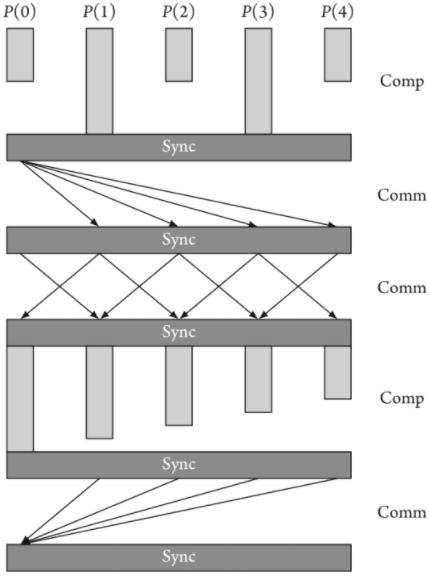
\includegraphics[scale=0.4]{Pic34.png}
		\caption{یک فرآیند \lr{BSP} با 5 ابرگام}
		\label{P34}
	\end{center}
\end{figure}

در شکل \ref{P34} یک فرآیند \lr{BSP} نشان داده شده است که در مجموع برای 5 مرحله ابرگام اجرا شده است. پردازنده‌های 0، 2 و 4 در مرحله اول، فقط به اندازه نصف پردازنده‌های 1 و 3 محاسبه انجام می‌دهند. بنابراین باید 50 درصد مواقع بیکار بمانند. این نکته مهم که در برنامه‌نویسی موازی به ویژه برنامه‌نویسی موازی از طریق \lr{BSP} برجسته است همان اطمینان از متعادل بودن بار محاسباتی بین پردازنده‌ها است. در ادامه کتابخانه‌‌هایی که مدل محاسباتی \lr{BSP} را پشتیبانی می‌کنند و امکانات آنها به طور مختصر آورده شده است.

کتابخانه نرم‌افزاری \lr{BSPy} در زبان برنامه‌نویسی پایتون عملکردهای کلیدی زیر را پشتیبانی می‌کند: 
\begin{itemize}
	\item 
	\lr{bsp.cores()}: درخواست تعداد کل پردازنده‌هایی که به صورت موازی کار می‌کنند
	\item
	\lr{bsp.pid}: درخواست شناسه پردازنده جاری   
	\item 
	\lr{bsp.send()}: ارسال پیام از این پردازنده به دیگری
	\item 
	\lr{bsp.move()}: انتقال پیام به خارج از صف «پیام‌های دریافت‌شده»
	\item 
	\lr{bsp.sync()}: شروع یک ابرگام جدید با همگام‌سازی همه پردازنده‌ها
\end{itemize}

کتابخانه نرم‌افزار دیگری وجود دارد که برای این منظور طراحی شده است و بسیار ساده است. کتابخانه \lr{BSPlib} از 20 نمونه اولیه تشکیل شده است که عملکرد و سرعت مشابه‌ای با \lr{MPI} ارائه می‌دهند. این کتابخانه امکان  ایجاد برنامه‌های موازی را مطابق با الگوی برنامه‌نویسی \lr{BSP} فراهم می‌کند و این امکان را می‌دهد که یک الگوریتم موازی را به شیوه‌ای بسیار ساختاریافته برنامه‌ریزی کرد و در نتیجه کدی خوانا و سریع بدست آورد. \lr{BSPlib} قبلاً برای چندین ابرکامپیوتر و کلاسترهایی از رایانه‌های شخصی پیاده‌سازی شده است، اما از آنجایی که محبوبیت کمتری نسبت به \lr{MPI} دارد، برای همه پلتفرم‌های سخت‌افزاری پیاده‌سازی نشده است. از آنجایی که مهندسان و ریاضیدانان همیشه بالاترین درصد توان محاسباتی را می‌خواهند، در نتیجه اجرای کارآمد یک برنامه مبتنی بر \lr{MPI} ضروری می‌باشد. در حال حاضر دو پیاده‌سازی اصلی از \lr{BSPlib} شامل \lr{Oxford BSP Toolset} و \lr{PUB} وجود دارد که برای پلتفرم‌های سخت‌افزاری خاص (\lr{Cray T3E} یا \lr{SGI Origin} و غیره) پیاده‌سازی شده‌اند. معماری کتابخانه نرم‌افزاری آنها برای استفاده از ویژگی‌های خاص سخت‌افزار بهینه شده است. بنابراین اگر سخت‌افزار/نرم‌افزار توسط یکی از این دو کتابخانه پشتیبانی نشود، باید از \lr{BSPonMPI} در ترکیب با کتابخانه \lr{MPI} استفاده کرد که بسیار سریع است. 

کتابخانه \lr{BSPonMPI} یک کتابخانه نرم‌افزاری مستقل برای توسعه برنامه‌های موازی به زبان برنامه‌نویسی \lr{C} است که استاندارد \lr{BSPlib}\cite{BSPLib} را پیاده‌سازی می‌کند و روی همه ماشین‌هایی که دارای \lr{MPI} هستند، اجرا می‌شود. این ویژگی اصلی این کتابخانه است که آن را از سایر کتابخانه‌ها مانند \lr{Oxford BSP Toolset} و \lr{PUB}\cite{PUB1,PUB2}\footnote{\lr{Paderborn University BSP }} متمایز می‌کند. \lr{MPI} یا \lr{Message Passing Interface} یک \lr{API} برای برنامه‌نویسی موازی می‌باشد که باید نوشتن یک برنامه موازی را آسان کند اما در عمل بسیار پیچیده است، زیرا این \lr{API} شامل صدها تابع می‌باشد. همچنین در حین برنامه‌نویسی موازی بر اساس \lr{MPI} باید مراقب بود که از خطاهای برنامه‌نویسی موازی معمولی مانند بن‌بست یا رفتار نامعین اجتناب شود. 

کتابخانه \lr{PyBSP} یک کتابخانه نرم‌افزاری برای توسعه محاسبات موازی \lr{BSP} است که هدف آن پشتیبانی از \lr{BSP} در پایتون با یک ماژول بسیار ساده پایتونی به نام \lr{bsp} می‌باشد. با استفاده از توابع موجود در این کتابخانه می‌توان پایتون را به یک \lr{BSP} واقعی تبدیل کرد. برخی از این توابع به شرح زیر می‌باشد:
\begin{itemize}
	\item 
	\lr{bsp.procCount()}: تعداد کل پردازنده‌ها را مشخص می‌کند
	\item 
	\lr{bsp.myProcID()}: شماره پردازنده جاری را مشخص می‌کند
	\item 
	\lr{bsp.fromObject(somePythonObject, 'name1')}: داده‌ها باید قبل از ارسال به سایر پردازنده‌ها بسته‌بندی شوند. با این دستور محتوای یک شی بسته‌بندی شده و بسته  \lr{"name1"} نامگذاری می‌شود.
	\item 
	\lr{bsp.fromNumpy(someNumpyArray, 'name2')}: این دستور محتوای یک آرایه \lr{numpy} را بسته‌بندی می‌کند و بسته  \lr{"name2"} نامگذاری می‌شود.
	\item 
	\lr{bsp.toProc(someProcID, 'name1')}: ارسال بسته \lr{"name1"} به پردازنده با شناسه‌ \lr{someProcID}
	\item 
	\lr{bsp.sync('some pass phrase')}:	دستور همگام‌سازی کلی برای شروع تبادل داده و منتظر ماندن برای آن است. عبارت \lr{'some pass phrase'} برای جلوگیری از همگام‌سازی‌های مختلف به یکدیگر است.
\end{itemize}

پکیج \lr{ScientificPython} مجموعه‌ای از ماژول‌های پایتون است که برای محاسبات علمی مفید است. در این مجموعه ماژول‌هایی برای هندسه پایه (بردارها، تانسورها، تبدیل‌ها، میدان‌های برداری و تانسوری)، کواترنیون‌ها، مشتقات خودکار، درون‌یابی (خطی)، چند جمله‌ای‌ها، آمار ابتدایی، برازش‌های حداقل مربعات غیرخطی، محاسبات واحد، فرترن- قالب‌بندی متن سازگار، تجسم سه‌بعدی از طریق \lr{VRML}، و دو ویجت \lr{Tk} برای نمودارهای خط ساده و مدل‌های قاب سیمی سه‌بعدی وجود دارد. همچنین رابط‌هایی برای کتابخانه\lr{MPI} (واسط ارسال پیام، برنامه‌نویسی موازی مبتنی بر پیام) و \lr{BSPlib} (برنامه‌نویسی موازی همگام مانعی) وجود دارد. اکوسیستم علمی پایتون بدون حفظ سازگاری با نسخه‌های قدیمی‌تر، با سرعتی سریع در حال تغییر است. از آغاز توسعه \lr{ScientificPython} در سال 1995، تغییرات مهمی در خود زبان پایتون بین \lr{Python 2.7} و \lr{Python 3} و همچنین تعداد زیادی تغییرات ناسازگار کوچکتر در کتابخانه \lr{NumPy} که \lr{ScientificPython} به آن وابسته است، رخ داده است که این پکیج با این تغییرات سازگار نیست. بنابراین \lr{ScientificPython} فقط با \lr{Python 2.7} و \lr{NumPy 1.8} قابل استفاده است.


\section{خلاصه}
در این فصل، مروری بر مفاهیم اولیه مورد نیاز در زمینه شبکه‌های تطبیقی توزیع‌شده و مدل‌های محاسباتی موازی برای درک بهتر مطالب این رساله ارائه شد. همچنین تاریخچه و برتری‌های مدل محاسباتی موازی‌سازی مانعی و امکانات نرم‌افزاری فراهم شده برای آن ارائه گردید. در ادامه در فصل آینده، کارهای پیشین و مرتبط به این رساله مطرح خواهند شد. 










\chapter{مروری بر کارهای پیشین}
\newpage
‎\renewcommand{\baselinestretch}{2}\normalsize‎
\label{Previous works_2}
در این فصل، پس از بیان یک مقدمه در زمینه فاکتورهای موثر بر کارآیی و همگرایی الگوریتم‌های یادگیری توزیع‌شده، راه‌حل‌های ارائه شده برای یادگیری توزیع‌شده، الگوریتم‌های یادگیری توزیع‌شده انتشاری و نقاط ضعف راه‌حل‌های موجود مرور خواهند شد. 

\section{مقدمه}
امروزه با افزایش حجم داده‌های پردازشی و همچنین نیاز به انجام محاسبات سنگین در بسیاری از حوزه‌ها، راه‌کارهای بسیاری برای پیاده‌سازی الگوریتم‌های توزیع‌شده به منظور تسریع فرآیند یادگیری و بهبود نرخ همگرایی ارائه شده است. انتخاب پلتفرم مناسب برای پیاده‌سازی یکی از مواردی است که تاثیر بسیار زیادی بر کارآیی الگوریتم دارد. الگوريتم‌هاي موازي بر روي پلتفرم‌هاي 1) سيستم حافظه اشتراكي (\lr{multi-core } يا \lr{many-core}) 2) سیستم حافظه اشتراکی توزیع‌شده 3) سیستم حافظه توزیع‌شده یا شبكه كامپيوتري پياده‌سازي می‌شوند \cite{lian2019}. هر یک از پلتفرم‌ها مزایا، کاربردها و معایبی دارند. 

مورد دیگر، مدل‌های محاسباتی موازی هستند که تاثیر بسیاری بر همگام‌سازي گره‌ها و کارایی الگوریتم‌ها دارند و هم روشی مفید برای هدایت طراحان الگوریتم‌های موازی و برنامه‌نویسان برای بهینه‌سازی کد و بهره‌برداری از ویژگی‌های سخت‌افزاری جدید ارائه می‌دهند. همچنین در حوزه سیستم‌های یادگیری توزیع‌شده به منظور تسریع عملیات و مدیریت بهتر بخش‌های مختلف محاسبات و ارتباطات و همچنین همگام‌سازي مناسب گره‌ها، پیاده‌سازی فرآیند یادگیری توزیع‌شده باید تحت یک مدل محاسباتی موازی از جمله  \lr{PRAM}، \lr{LogP}، \lr{BSP} و \lr{MapReduce} انجام شود. مدل محاسباتی \lr{PRAM} یک مدل حافظه اشتراکی است و به دلیل محدودیت در تعداد پردازنده‌ها و بالا بودن هزینه ارتباطات نسبت به هزینه محاسبات برای پیاده‌سازی همه جانبه مناسب نیست. مدل محاسباتی \lr{LogP} مدل برنامه‌نویسی ندارد و ارتباطات پردازنده‌ها در آن به صورت یک نمای محلی بر اساس عملکرد هر جفت پردازنده است. در مقاله \cite{BSP2012} تفاوت‌های بین چارچوب نگاشت-کاهش و مدل محاسباتی \lr{BSP} مورد بحث قرار گرفته‌اند و این واقعیت برجسته شده است که الگوریتم‌های \lr{BSP} به دلیل نیاز به ذخیره‌سازی و دسترسی به داده‌ها در چندین ابرگام، در صورتی که تعداد ابرگام‌ها ثابت نباشد، نمی‌توانند به طور موثر با استفاده از چهارچوب نگاشت-کاهش پیاده‌سازی شوند. این مورد به دلیل ماهیت چارچوب نگاست-کاهش است که اجازه ذخیره‌سازی داده بین دورها را نمی‌دهد، اما الگوریتم‌های \lr{BSP} مستلزم این هستند که به این داده‌ها بین چنین دورهایی دسترسی داشته باشند. همچنین، آنها نشان دادند که مدل \lr{BSP} می‌تواند برای مدل‌سازی الگوریتم‌های نگاشت-کاهش با هزینه جانبی یکسان برای سیستم‌های معمولی با تعداد پردازنده‌های یکسان استفاده شود. بنابراین، مشخص شده است که \lr{MapReduce} باید صرفاً به عنوان یک چارچوب پیاده‌سازی با \lr{BSP} برای طراحی الگوریتم‌ها استفاده شود. با این حال، برای کارهایی با زمان اجرا ناشناخته، \lr{MapReduce} همچنان باید استفاده شود زیرا \lr{BSP} دارای قابلیت تعادل بار پویا نیست. به عنوان مثال، فریمورک محاسبات توزیع‌شده\lr{Apache hama} از مدل \lr{BSP} استفاده می‌کند و گره‌ها می‌توانند با یکدیگر ارتباط برقرار کنند، در حالیکه فریمورک \lr{Apache Hadoop} مبتنی بر چارچوب نگاشت-کاهش است و گره‌ها در انتهای هر دور تنها  مجاز به ارتباط با پردازنده مرکزی هستند. 

مورد سوم، پیاده‌سازی الگوریتم‌های یادگیری توزیع‌شده به صورت متمرکز و غیرمتمرکز است. روش متمرکز یک الگوی پیاده‌سازی است که که در آن تعداد زیادی از گره‌ها با یک یا چند سرور مرکزی هماهنگ می‌شوند تا یک مدل را بدون به اشتراک گذاشتن داده‌های اولیه و خام خود یاد بگیرند. گره‌ها داده‌های میانی از جمله گرادیان‌ها، بردارهای تخمین‌زده و غیره را به سرورهای مرکزی ارسال می‌کنند و با استفاده از نتایج میانگین‌گیری شده دریافتی از سرورها ادامه محاسبات خود را انجام می‌دهند. در این نوع پیاده‌سازی چنین تبادلات داده‌ای دائما بین گره‌ها و سرورهای مرکزی انجام می‌شود. روش غیرمتمرکز الگوی پیاده‌سازی دیگری برای ماشین‌های یادگیری توزیع‌شده  بدون حضور سرور مرکزی است که هر گره بعد از انجام محاسبات محلی، داده‌های میانی خویش را با یک یا تعدادی گره همسایه دیگر تبادل کرده و ادامه محاسبات را بر اساس داده‌های دریافتی انجام می‌دهد. در الگوریتم‌های یادگیری توزیع‌شده غیرمتمرکز  استراتژی‌های متفاوتی برای انتخاب گره‌های همسایه ارائه شده است. 

مورد موثر چهارم بر کارایی الگوریتم‌های یادگیری توزیع‌شده، روش همگام‌سازي یا مکانیزم کنترل مانع بین گره‌ها است.  در حال حاضر، روش‌های کنترل مانع را می‌توان به طور کلی به سه مکانیزم موازی غیرهمگام \footnote{\lr{Asynchronous Parallel}} (\lr{ASP})، مکانیزم موازی همگام با کهنگی \footnote{\lr{Stale Synchronous Parallel}}(\lr{SSP}) و مکانیزم موازی همگام مانعی \footnote{\lr{Bulk Synchronous Parallel}} (\lr{BSP}) دسته‌بندی کرد \cite{NIPS2012}. مکانیزم \lr{BSP} یک طرح قطعی است که در آن گره‌ها یک مرحله محاسباتی را انجام می‌دهند و به دنبال آن یک مرحله همگام‌سازی یا ارتباطات برای تبادل به‌روزرسانی‌ها را انجام می‌دهند. این روش اطمینان می‌دهد از طریق جلوگیری از رفتن هر گره به مرحله بعدی تا زمانی که همه گره‌ها بتوانند محاسبات را به اتمام برسانند، همه گره‌ها در یک تکرار محاسباتی یکسانی قرار خواهند داشت. علاوه بر این، اثرات محاسبات فعلی برای گره‌ها تا زمانی که مانع انجام نشده است، قابل مشاهده نیست. با توجه به اینکه تضمین‌های صحت برنامه سریال برای برنامه‌های \lr{BSP} اغلب قابل تحقق است، در نتیجه \lr{BSP} قوی‌ترین روش کنترل مانع خواهد بود \cite{Ho2013}. متأسفانه \lr{BSP} یک نقطه ضعف بزرگ دارد. از آنجایی که گره‌ها باید منتظر بمانند تا کار دیگران به پایان برسد، در صورت وجود گره‌هایی با قدرت محاسباتی کمتر در یک شبکه ناهمگن \cite{NIPS2012} و یا گره‌هایی که به دلیل عوامل تصادفی و غیرقابل پیش‌بینی به زمان بیشتری برای تکمیل یک مرحله نیاز دارند، کارایی محاسبات در این مدل براساس کندترین ماشین تعیین می‌گردد. این امر منجر به کاهش چشمگیر عملکرد سیستم می‌شود. به طور کلی، \lr{BSP} دقت محاسباتی بالایی دارد اما در محیط‌های ناهمگن از کارایی پایین رنج می‌برد.

مکانیزم \lr{ASP} ساده‌ترین مدل است که هیچ همگام‌سازی بین گره‌ها رخ نمی‌دهد. این مکانیزم نقطه متقابل مکانیزم کنترل مانع \lr{BSP} است و اجازه می‌دهد محاسبات با حداکثر سرعت ممکن از طریق اجرای کاملا غیرهمگام گره‌ها انجام شود. در محیط‌های محاسباتی همگن، که در آن گره‌ها پیکربندی‌ مشابهی دارند، مکانیزم \lr{ASP} هم‌گرایی سریعی دارد و بالاترین توان عملیاتی تکرار را نتیجه می‌دهد. اما در حالت کلی، این غیرهمگامی باعث تاخیر در به‌روزرسانی و اعمال نویز و خطا در محاسبات می‌شود. در نتیجه، مکانیزم \lr{ASP} از کاهش کیفیت تکرار رنج می برد و حتی ممکن است در برخی از محیط‌ها واگرا شود. به طور کلی، \lr{ASP} سرعت‌های بسیار خوبی را در همگرایی ارائه می‌دهد، اما خطر واگرایی بیشتری به خصوص در محیط‌های ناهمگن دارد.

مکانیزم \lr{SSP} یک مدل همگام محدود شده است که می‌تواند به عنوان یک مدل \lr{BSP} سست شده در نظر گرفته شود. به‌جای اینکه همه گره‌ها را ملزم کند در یک تکرار باشند، سیستم تصمیم می‌گیرد که آیا گره ممکن است بر اساس میزان عقب‌تر بودن از کندترین گره، (یک کهنگی محدود از پیش تعریف‌شده) کار کند. به طور خاص، گره‌ای که بیش از \lr{s } تکرار از سریعترین گره عقب باشد، خیلی کند در نظر گرفته می‌شود. اگر چنین گره‌ای وجود داشته باشد، سیستم گره‌های سریع‌تر را متوقف می‌کند تا زمانی که گره کند به آنها برسد. این \lr{s} به عنوان پارامتر کهنگی شناخته می‌شود. این پارامتر به مکانیزم \lr{SSP} اجازه می‌دهد تا همگرایی قطعی را تضمین کند \cite{Ho2013}. به عبارت‌ دیگر، این مکانیزم تفاوت تعداد تکرارها بین سریعترین و کندترین گره‌ها را کنترل می‌کند و با مجبور کردن سریعترین گره به صبر تا زمانی‌که از آستانه فراتر نرود، آن را در محدوده آستانه قرار می‌دهد. مکانیزم \lr{SSP} یک راه‌حل کوتاه‌بینانه ارائه می‌دهد، زیرا ظرفیت محاسباتی هر گره (یعنی سرعت آن) را در نظر نمی‌گیرد و فقط به تعداد تکرارهایی که هر گره انجام داده است ، توجه می‌کند. به طور کلی، مکانیزم \lr{SSP} مصالحه خوبی بین \lr{BSP} کاملاً قطعی و همگام و \lr{ASP} کاملاً غیرهمگام ارائه می‌کند. با تنظیم پارامتر کهنگی $s = 0 $ در \lr{SSP}، روش \lr{BSP} را خواهیم داشت. درحالی‌که با تنظیم $s=\infty$ مکانیزم \lr{ASP} اجرا می‌شود. شکل \ref{p26} یک مقایسه کلی از سه مکانیزم کنترل مانع بر اساس میزان سازگاری (سرعت همگرایی) و سرعت (بازده) یادگیری، به تصویر کشیده است. 

\begin{figure}
	\begin{center}
		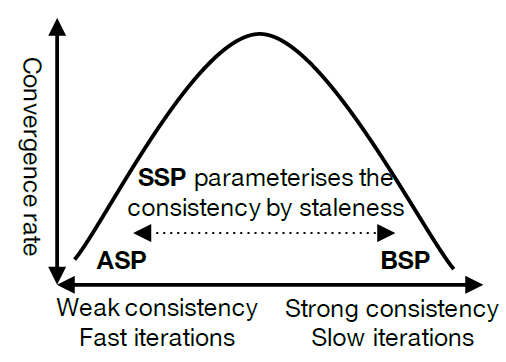
\includegraphics[scale=0.6]{Pic26.png}
		\caption{مقایسه سه مکانیزم کنترل مانع \cite{Zhao2021}}
		\label{p26}
	\end{center}
\end{figure}

به طور خلاصه در شکل \ref{Barrier} تکنیک‌های همگام‌سازی و کنترل مانع که تا کنون معرفی شده‌اند به همراه تکنیک کنترل مانع پیشنهادی در این رساله به نام تکنیک همگام منطقه‌ای \lr{FBSP} آورده شده است. تکنیک غیرهمگام احتمالی \lr{PSP} نیز در بخش \ref{CmpMld} به عنوان یک راه‌کار مبتنی بر مدل محاسباتی متمرکز تشریح خواهد شد.

\begin{figure}
	\begin{center}
		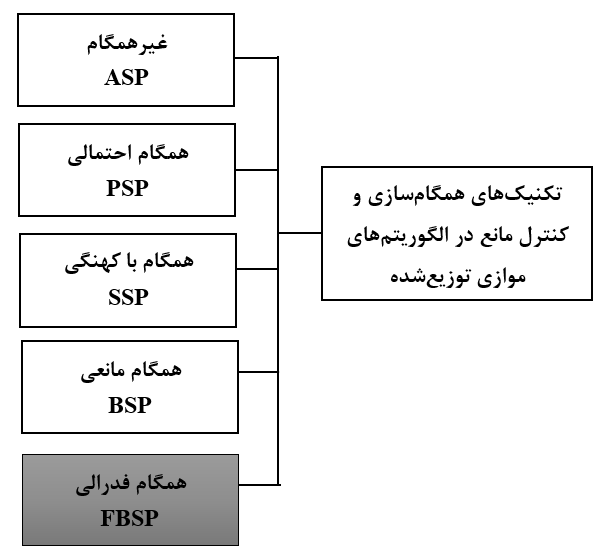
\includegraphics[scale=1.2]{BarrierTypes_.PNG}
		\caption{مکانیزم‌های کنترل مانع موجود و مکانیزم پیشنهادی در این رساله}
		\label{Barrier}
	\end{center}
\end{figure}

\section{بیان راه‌حل‌های موجود برای یادگیری توزیع‌شده}

در سیستم‌های حافظه اشتراکی همه پردازنده‌ها به یک حافظه مشترک دسترسی دارند و از نظر سخت‌افزاری همه پردازنده‌ها از طریق یک گذرگاه به حافظه فیزیکی مشترک دسترسی دارند. این پردازنده‌ها می‌توانند به طور مستقل کار کنند در حالی که همه آنها به یک حافظه دسترسی دارند. هر گونه تغییر در متغیرهای ذخیره شده در حافظه توسط همه پردازنده‌ها قابل مشاهده است. در صورتی که پردازنده $i$ در حال استفاده از یک متغیر باشد و به طور هم‌زمان پردازنده $j$ با دسترسی به همان متغیر بر روی آن تغییری اعمال نماید، در واقع پردازنده $i$ با نسخه قدیمی آن متغیر کار می‌کند. این سیستم‌ها از مشکل خواندن‌های ناسازگار رنج می‌برند. اكثر الگوریتم‌های موازی مطرح شده در سیستم‌های حافظه اشتراکی نیاز به همگام‌سازي پردازنده‌ها و يا قفل‌کردن برای کنترل دسترسی هم‌زمان پردازنده‌ها به حافظه اشتراکی دارند. این موارد سبب پایین آمدن کارایی طرح‌ها و الگوریتم‌های موازی مي‌شود. با توجه به اینکه قفل‌های نرم‌افزاری هزینه‌های بسیار زیادی دارند، در حالت ایده‌آل طرحی مناسب است که بدون انتظار و قفل باشد. 
در نوعی دیگر از سیستم‌های حافظه که با نام ماشین‌های دسترسی حافظه غیریکنواخت \lr{NUMA}\footnote{\lr{Non-Uniform Memory Access}} یا سیستم‌های حافظه اشتراکی توزیع‌شده شناخته می‌شوند، تعدادی پردازنده \lr{CPU} با هسته‌های بسیار وجود دارد که زمان دسترسی به حافظه توسط هر پردازنده کاملا بستگی به مکان قرار گرفتن حافظه نسبت به آن دارد. یک پردازنده می‌تواند به حافظه محلی خود سریعتر از حافظه غیرمحلی (حافظه محلی پردازنده دیگر یا حافظه مشترک بین پردازنده‌ها) دسترسی پیدا کند. بزرگترین مزیت \lr{NUMA} انتقال سریع داده‌ها و تاخیر کمتر در سیستم‌های چندپردازشی است؛ بنابراین این سیستم‌ها برای برنامه‌های بلادرنگ و حیاتی به کار می‌روند.
در سیستم‌های حافظه توزیع‌شده هر پردازنده حافظه محلی خود را دارد و پردازنده‌ها از طریق یک شبکه با هم در ارتباط هستند. به عبارتی، حافظه توزیع‌شده در مفهوم سخت‌افزاری به حالتی اطلاق می‌شود که پردازنده‌ها فقط می‌توانند حافظه محلی خود را مستقیما ببیند و تنها از طریق شبکه می‌توانند به حافظه پردازنده‌های دیگر دسترسی داشته باشند. در این مدل سیستم‌ها انواع مختلف پردازنده‌ها را می‌توان تجربه کرد.

الگوریتم‌های ارائه شده برای یادگیری توزیع‌شده بر روی پلتفرم‌هاي حافظه اشتراکی، حافظه اشتراکی توزیع‌شده \lr{NUMA} و حافظه توزیع‌شده پیاده‌سازی شده‌اند. در شکل \ref{Cat1} دسته‌بندی راه‌حل‌های ارائه شده برای یادگیری توزیع‌شده براساس چهار دیدگاه مختلف انجام شده است: 1) نوع سیستم حافظه اشتراکی/توزیع‌شده، 2) استفاده/عدم استفاده از مدل محاسباتی، 3) متمرکز/غیرمتمرکز بودن و 4) همگام/غیرهمگام بودن مکانیزم کنترل مانع. در شکل \ref{Cat1} جایگاه رویکرد پیشنهادی \lr{FBSP} در این رساله نیز نشان داده شده است. 

 \begin{figure}
	\begin{center}
		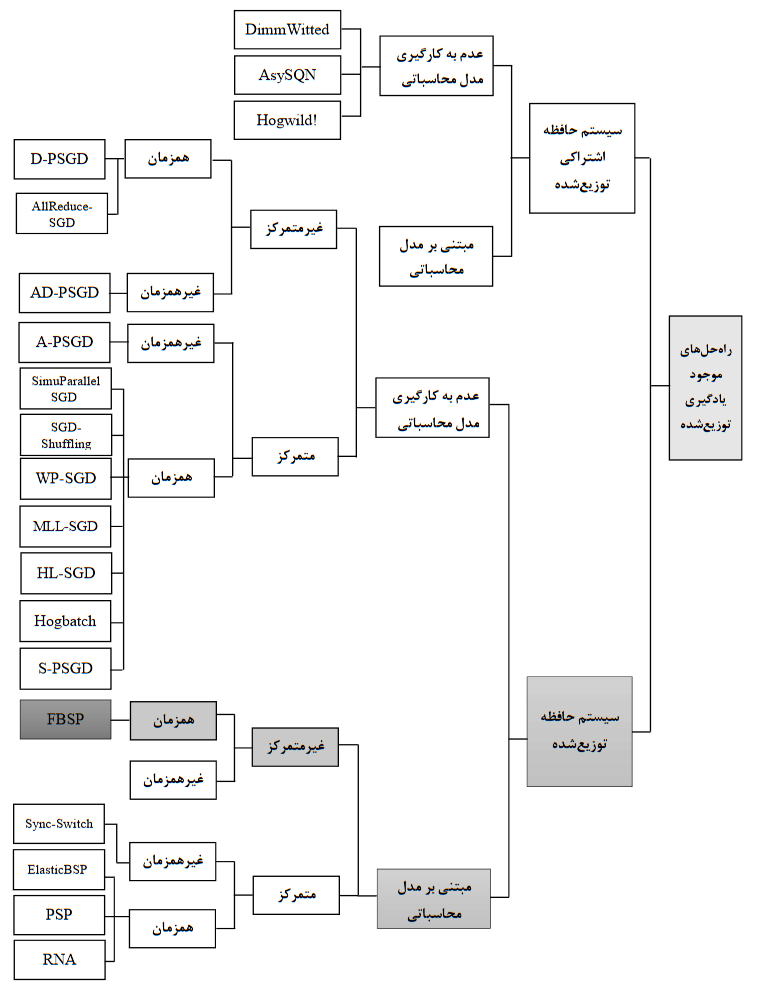
\includegraphics[scale=1.2]{CatApprochs_1.PNG}
		\caption{دسته‌بندی راه‌حل‌های موجود برای یادگیری توزیع‌شده}
		\label{Cat1}
	\end{center}
\end{figure}

در بخش‌های \ref{WthCmpMdl} و \ref{CmpMld} راه‌حل‌های ارائه شده در حوزه یادگیری توزیع‌شده با جزئیات بیشتری شرح داده خواهند شد.  هر یک از راه‌حل‌های معرفی شده در این دو بخش از الگوریتم یادگیری یا به عبارتی روش به‌روزرساني متفاوتی در فرآیند یادگیری خویش بهره می‌گیرد. در سال‌های اخیر، الگوریتم‌های انتشار بر روی شبکه‌های تطبیقی توزیع‌شده به دلیل همگرایی سریع و رسیدن به میانگین خطا کمتر در حالت پایدار و همچنین مقیاس‌پذیری، غیرمتمرکز بودن و مقاومت این نوع شبکه‌ها در برابر خرابی گره‌ها و یال‌ها بسیار مورد توجه محققان قرار گرفته‌اند. شبکه‌های تطبیقی توزیع‌شده برای یادگیری مجموعه داده‌های بزرگ با بهره‌مندی از قدرت همکاری میان گره‌ها مناسب می‌باشند. در بخش \ref{DfsnAlg} الگوریتم‌های یادگیری تطبیقی انتشار معرفی‌شده مورد بررسی قرار می‌گیرند و یک دسته‌بندی از آنها نیز ارائه می‌گردد.

\subsection{راه‌حل‌های توزیع‌شده بدون مدل محاسباتی}\label{WthCmpMdl}


در \cite{Hog12011} یک استراتژی ساده برای اجرای \lr{SGD} به صورت موازی و بدون قفل به نام \lr{Hogwild! } ارائه شده است که پردازنده‌ها (گره‌ها) اجازه دسترسی یکسان به حافظه اشتراکی را دارند و می‌توانند اجزای مجزای حافظه را به دلخواه خود به‌روزرسانی کنند. از آنجایی که پردازنده‌ها می‌توانند تغییرات پردازنده‌های دیگر را بازنویسی کنند، الگوریتم بدون قفل ممکن است دچار مشکل شود. در این مقاله نشان داده شده است که وقتی دسترسی به داده‌ها به صورت خلوت  باشد یا به عبارتی در هر گام فقط بخش کوچکی از بردار پارامتر به‌روزرسانی شود، بازنویسی حافظه توسط پردازنده‌های مختلف به ندرت رخ می‌دهد و در صورت بروز در محاسبات خطا دیده خواهد شد. در این استراتژی یک تسریع تقریبا خطی با توجه به تعداد پردازنده‌ها برای مسائل یادگیری خلوت از نظر تئوری و تجربی ارائه شده است اما همان طور که بیان شد تنها برای مسائل بهينه‌سازي خلوت قابل اعمال است. تابع هزینه خلوت در استراتژی \lr{Hogwild!} به صورت زیر تعریف می‌شود:

\begin{equation}\label{e18}
	f(w)=\sum_{e\in E}f_e(w,x_e)
\end{equation}

که بردار پارامتر $w$ در حافظه اشتراكي ذخيره می‌شود و توسط تمام پردازنده‌ها در دسترس است. $e$ زیرمجموعه کوچکی از $\{1, 2, ...,M\}$ است و $x_e$ مقادير بردار ورودی $x$ با توجه به نقاط انتخاب شده در $e$ را نشان می‌دهد.

در مقاله \cite{Zin2010} یک الگوریتم \lr{SGD} موازی بر اساس یک استراتژی تک-میانگین‌گیری  به نام \lr{SimuParallel SGD } ارائه شده است و مبنا را بر مدل داده-موازی گذاشته است. به عبارتی \lr{m } نمونه داده بین \lr{k} پردازنده تقسیم شده و در هر تکرار $t$ هر پردازنده \lr{i} به صورت مستقل و بدون هیچ تبادل و همکاری با دیگر پردازنده‌ها، گرادیان کاهشی تصادفی را با توجه به داده‌ $c^{i,t}$ و بردار پارامتر $w_{i,t}$ محاسبه می‌کند. زمانی که اجرای تمام پردازنده‌ها به پایان رسید، در نقطه همگام‌سازی نتایج تجمیع و سپس میانگین آنها به عنوان نتیجه نهایی در نظر گرفته می‌شود.

الگوریتم گرادیان کاهشی تصادفی موازی همگام\footnote{\lr{Synchronous Parallel Stochastic Gradient Descent (S-PSGD)}}  \lr{(S-PSGD)} یک روش یادگیری توزیع‌شده موازی است که در مقاله \cite{Mini2016} برای حل توابع هزینه غیرمحدب و در \cite{dekel2012} برای حل توابع هزینه محدب معرفی شده است. پیاده‌سازی این الگوریتم به صورت متمرکز و با حضور یک سرور پارامتر  \footnote{\lr{Parameter server}} انجام شده است. در هر گام هر گره بردار پارامتر را از سرور پارامتر خوانده و گرادیان تصادفی دسته‌ای را محاسبه می‌کند. سپس گره‌ها گرادیان‌های خود را به سرور پارامتر ارسال کرده و بعد از همگام‌سازی، با استفاده از میانگین گرادیان‌ها بردار پارامتر ذخیره‌شده در سرور پارامتر به‌روزرسانی می‌شود. به دلیل وجود گام همگام‌سازی، اکثر گره‌ها باید در حالت انتظار قرار بگیرند تا کار آهسته‌ترین گره به اتمام برسد. در این روش هزینه گام‌ همگام‌سازی $O(N)$ است. زمانی که $N$ بزرگ باشد، سبب هزینه‌های ارتباطی بالا در سرور پارامتر می‌شود. 

در مقاله \cite{nccl} برای پیاده‌سازی الگوریتم \lr{AllReduce-SGD } از قانون به روزرسانی دقیقاً مشابه \lr{S-PSGD} در هر تکرار استفاده شده است. هیچ سرور پارامتری در این الگوریتم وجود ندارد. گره‌ها با یک شبکه حلقه بهم متصل شده‌اند و هر گره نسخه محلی از مدل را نگه می‌دارد. در هر تکرار، هر گره گرادیان دسته‌ای را محاسبه کرده و سپس از \lr{AllReduce} برای همگام‌سازی گرادیان‌ها استفاده می‌کنند. در نهایت هر گره میانگین همه گرادیان‌ها را بدست می‌آورد. این الگوریتم در شبکه‌ای با تاخیر بالا کند عمل خواهد کرد. در پایان تکرار، مدل محلی هر گره با میانگین گرادیان‌ها به‌روز می‌شود. به دلیل وجود همگام‌سازی در هر تکرار، زمان بیکاری همانند الگوریتم \lr{S-PSGD} بالا است. 

ماشین‌های  \lr{NUMA}\footnote{\lr{Non-Uniform Memory Access}} از تعدادی پردازنده \lr{CPU} با هسته‌های زیاد تشکیل شده‌اند. به عبارت دیگر مدلی از طراحی سخت‌افزاری است که در سرورهایی با چند \lr{CPU} استفاده می‌شود و استفاده از حافظه توسط یک پردازنده \lr{CPU} کاملا بستگی به مکان قرار گرفتن حافظه نسبت به آن دارد. استراتژی  \lr{DimmWitted} \cite{DimmWitted} یک تحلیل آماری بر روی روش‌های تکثیر مدل و داده و همچنین شیوه‌های دسترسی به داده‌ها در حافظه اصلی يك ماشين \lr{NUMA} ارائه داده است. در واقع گره‌ها بر روی گره‌های یک ماشین \lr{NUMA} پیاده‌سازی شده‌اند و همگام‌سازي مدل‌ها بر روي گره‌ها انجام می‌شود. این همگام‌سازی تا زمانی‌ که مانع عبور و مرور داده‌ها در حافظه اصلی نشود، سودمند است. به منظور همگام‌سازی در این استراتژی، یک نخ در هر گره به صورت متناوب مدل‌های روی تمام گره‌ها را می‌خواند و پس از میانگین‌گیری نتایج، کپی مدل ‌در گره را به‌روزرسانی می‌‌کند.

در مقاله \cite{lian2019} با استفاده از دو پلتفرم حافظه اشتراکی و شبکه کامپیوتری (حافظه توزیع‌شده) دو الگوریتم \lr{SGD} توزیع‌شده موازی غیرهمگام\footnote{\lr{Asynchronous}} به صورت متمرکز برای حل مسائل بهینه‌سازی غیرمحدب معرفی شده است. این الگوریتم با نام \lr{A-PSGD } شناخته شده‌است که در مقاله \cite{ag2011} از این الگوریتم برای حل مسائل محدب نیز استفاده شده است. در الگوریتم \lr{AsySG-con} \cite{lian2019} که بر روی پلتفرم شبکه‌ کامپیوتری پیاده‌سازی شده است، بردار پارامترها بر روی سرور مرکزی قرار دارد و در طول گام به‌روزرسانی، گره‌ها اجازه دسترسی به بردار پارمترها را ندارند. در نتیجه فرآیند خواندن بردار سازگار خواهد بود. برای ایجاد ارتباط بین گره‌ها و سرور مرکزی از کتابخانه \lr{MPICH} کمک گرفته شده است. برای پياده‌سازي الگوریتم‌های غيرهمگام، از یک پارامتر کهنگی\footnote{\lr{Staleness}}  استفاده می‌شود و مقادير قديمي بردار پارامتر براي ارزيابي گراديان تصادفي سایر گره‌ها به‌کار گرفته می‌شود. هر گره داده‌های نمونه را به صورت دسته‌های \lr{M}تایی تصادفی دریافت کرده و پس از محاسبه گرادیان آن را به سرور مرکزی ارسال می‌کند. سرور مرکزی با قبول یک میزان کهنگی $\tau _{k,m}$ در پارامترهای دریافتی از گره‌های شبکه به‌روزرسانی بردار پارامتر $w_{k+1}$ را انجام می‌دهد. 

\begin{equation}\label{e23}
	w_{k+1}=w_k-{\gamma}_k \sum_{m=1}^{M}G(x_{k-\tau_{k,m}},\xi_{k,m})
\end{equation}

میزان کهنگی گرادیان‌های دریافتی از گره نباید از یک حدی بیشتر باشد. زیرا همگرایی الگوریتم را به شدت کاهش می‌دهد و در بعضی مواقع سبب واگرایی آن می‌شود. براي داشتن همگرايي مناسب، میزان کهنگی نبايد زياد بزرگ باشد و یک حدآستانه‌ به صورت $\max_{k,m} \tau _{k,m}\le T$ در نظرگرفته شود \cite{Avron2014}.

در الگوریتم \lr{AsySG-INcon} \cite{lian2019} که بر روی پلتفرم حافظه اشتراکی پیاده‌سازی شده است، بردار پارامتر \lr{w} بر روی حافظه اشتراکی قرار می‌گیرد و هر گره بردار پارامتر را از حافظه خوانده و در حافظه محلی خود قرار می‌دهد و با استفاده از داده‌های نمونه و $\hat{w ̂}$ (مقدار خوانده شده از حافظه اشتراکی)  مقدار گرادیان $G(\hat{w}_k;\xi_k)$ را به صورت محلی محاسبه می‌کند. سپس بردار پارامتر $w$ در حافظه اشتراکی بدون قفل نرم‌افزاری به صورت زیر به‌روزرسانی می‌شود.
\begin{equation}\label{e24}
	(w_{k+1})_{i_k}=(w_k)_{i_k}-\gamma \sum_{m=1}^{M}(G(\hat{w}_{k,m},\xi_{k,m}))_{i_k} 
\end{equation}

که $i_k\in \{{1,2,…,M}\}$ یک اندیس تصادفی انتخاب شده برای به‌روزرسانی توسط گره \lr{k} و \lr{n} طول بردار پارامتر را نشان می‌دهد. الگوریتم \lr{A-PSGD } بر روی حافظه اشتراکی از مشکل خواندن‌های ناسازگار رنج می‌برد. راه‌حل استفاده شده برای غلبه بر این مشکل برگرفته از روش ارائه شده در \cite{Avron2014} می‌باشد. با مانیتور کردن مقدار بردار پارامتر در حافظه اشتراکی و استفاده از تعریف  $w_k$ به صورت زیر تا حدی این مشکل را می‌توان برطرف کرد:
\begin{equation}\label{e25}
	\hat{w}_k=w_k-\sum_{j\in J(k)} (w_{j+1}-w_j) 
\end{equation}

\begin{equation}\label{e26}
	J(k)\subset {k-1,...,k-T}, \quad \lvert J(k)\rvert\le T
\end{equation}

مجموعه $J(k)$ در رابطه \ref{e26} برای مانیتور کردن مقدار بردار پارامتر  در حداکثر $T$ گره دیگر است. 

زمانی‌که شرایط شبکه مساعد باشد، روش‌های \lr{SGD} موازی توزیع‌شده تسریع مشابه‌ای خواهند داشت و تفاوت این روش‌ها زمانی مشخص می‌شود که شبکه‌ای با پهنای باند کم و در نتیجه تاخیر بالا داشته باشیم. در الگوریتم \lr{D-PSGD} \cite{Lian20171} با حذف سرور مرکز سعی شده است یک \lr{SGD} موازی غیرمتمرکز همگام برای کاهش بار ترافیکی سرور و برطرف کردن معایب الگوریتم‌های قبلی معرفی شود. یکی از معایب این الگوریتم هزینه بالای همگام‌سازی گره‌ها در شبکه است. برای توزیع دادها می‌توان کل داده‌ها را در اختیار همه گره‌ها قرار داد یا داده‌ها را به شکلی مناسب پارتیشن‌بندی کرد و هر پارتیشن را در اختیار یک گره قرار داد. برای پیاده‌سازی این الگوریتم از چارچوب‌کاری یادگیری عمیق ماکروسافت \lr{CNTK} و کتابخانه \lr{Torch} استفاده شده است. 

در مقاله \cite{lian2018} الگوریتم غیرمتمرکز غیرهمگام  \lr{AD-PSGD } برای یادگیری موازی توزیع‌شده معرفی شده و معایب رویکردهای قبلی را برطرف کرده است. برای هر گره \lr{i} یک نخ محاسباتی (برای انجام محاسبات گرادیان‌ها و به‌روزرسانی وزن‌ها) و یک نخ ارتباطی (برای برقرار ارتباط بین گره \lr{i} و یک همسایه تصادفی و ترکیب بردار وزن‌ آنها) با یک بافر مشترک \lr{g} تعریف شده است که به ترتیب بر روی \lr{GPU} و \lr{CPU} اجرا می‌شوند. پردازنده‌های \lr{GPU} به طور پيوسته گراديان‌ها را محاسبه و نتايج را بدون توجه به اينكه ميانگين‌گيري رخ مي‌دهد يا خير، در بافر پردازنده‌های \lr{CPU} قرار مي‌دهند. در این مقاله گره‌ها به دو دسته فعال و غیرفعال تقسیم می‌شوند. به منظور جلوگیری از بن‌بست در تبادل و میانگین‌گیری بردارهای پارامتر دو گره انتخاب‌ می‌شود، به طوریکه یک گره فعال همسایه‌اش را تنها از مجموعه گره‌های غیرفعال می‌تواند انتخاب کند. به منظور مدیریت فرآیند یادگیری غیرهمگام از یک تکنیک کهنگی استفاده شده است. 

در صورتی‌که گره‌های شرکت‌کننده در فرایند یادگیری توزیع‌شده از لحاظ قدرت محاسباتی و پردازشی با یکدیگر متفاوت باشند، پردازنده‌ها با عملکرد پایین تاثیر منفی بر نتیجه نهایی خواهند گذاشت. در \cite{WP2020} یک الگوریتم گرادیان کاهشی موازی وزن‌دار به نام \lr{WP-SGD } معرفی شده است که بردارهای پارامتر گره‌ها به صورت وزن‌دار برای تولید نتیجه نهایی با یکدیگر ترکیب می‌شوند. وزن اختصاص داده شده به بردار پارامتر هر گره بر اساس تاخیر بین آن و سریع‌ترین گره تعریف شده است.

در مقاله \cite{Ma2019} دو روش موازی‌سازی \lr{SGD} همگام و \lr{SGD} غیرهمگام با استفاده از معماری‌های‌ محاسباتی مختلف در یک سیستم واحد پیاده‌سازی شدند و تاثير آنها بر روي كارايي سخت افزاري و زمان همگرايي در حالت‌هاي مختلف داده و توابع زیان متفاوت مورد بررسي قرار گرفته است. آن‌ها به این نتیجه دست یافتن که انتخاب بين نوع معماری محاسباتی و روش به‌روزرسانی مدل  به نوع کار و ويژگي داده‌ها وابسته است. در روش \lr{SGD} همگام، يك نخ مسئول به‌روزرساني مدل است. اين روش سبب محدود شدن اجراي موازي داخل الگوریتم مي‌شود. بهترین انتخاب برای موازی‌سازی عبارت جبرخطي، گراديان تابع زیان در مرحله محاسبه گراديان می‌باشد که براي تسريع محاسبات، پياده‌سازي‌هاي موازي كارا از كتابخانه‌هاي جبرخطي بهينه‌شده همچون کتابخانه \lr{ViennaCL} استفاده مي‌شود. این کتابخانه هم برای داده‌های خلوت و هم داده‌های متراکم کاربرد دارد. در صورتی‌که کتابخانه تنسورفلو و دیگر چهارچوب‌های کاری یادگیری عمیق تنها داده‌های متراکم را پشتیبانی می‌کنند و نمی‌توانند مدل‌های با ابعاد خیلی بالا را مدیریت کنند. 

یک الگوریتم \lr{SGD} توزیع‌شده بر اساس روش‌های بُرزدن محلی\footnote{\lr{Local shuffling}}  و سراسری\footnote{\lr{Global shuffling}}  با استفاده از یک گره مرکزی در مقاله \cite{MENG201946} ارائه شده است. بُرزدن یکی از روش‌های رایج پردازش داده است که برای حل مسائل بزرگ یادگیری ماشین از تقسیم‌بندی داده‌ها در طول چندین ماشین یا نخ کاربرد دارد. در الگوریتم ارائه شده، داده‌های آموزشی برزده می‌شوند و سپس داده‌ها به صورت زیرمجموعه‌های غیرهمپوشان تقسیم شده و هر زیرمجموعه به یک گره اختصاص می‌یابد. بعد از انجام فرآیند یادگیری در هر تکرار، مجددا بُرزدن به صورت محلی یا سراسری انجام می‌شود. اگر بُرزدن به صورت سراسری باشد، بعد از بُرزدن داده‌ها مجدد در هر تکرار تقسیم‌بندی داده‌های آموزشی به صورت زیرمجموعه‌های غیرهمپوشان انجام می‌شود اما اگر بُرزدن به صورت محلی انجام شود، دیگر نیازی به تقسیم‌بندی مجدد داده‌های آموزشی نیست. نویسندگان مقاله نشان دادند که اگر عملیات بُرزدن مستقل باشد، بُرزدن سراسری معادل نمونه‌گیری بدون جایگزینی است و آن‌ها همگرایی الگوریتم \lr{SGD} توزیع‌شده به روش بُرزدن محلی و سراسری را برای مسائل غیرمحدب اثبات کردند. نرخ همگرایی برای بُرزدن محلی کندتر از بُرزدن سراسری است، زیرا اگر ارتباطی بین داده‌های تقسیم شده وجود نداشته باشد، برخی اطلاعات را از دست خواهیم داد.

الگوریتم مرتبه دوم \lr{AsySQN} \cite{tong2020} یک الگوریتم موازی غیرهمگام براساس روش شبه نیوتن تصادفی است که مبتنی بر یک پلتفرم حافظه اشتراکی برای حل مسائل بدشرط ارائه شده است. در الگوریتم \lr{AsySQN} براساس تکنیک‌های حافظه مدرن، از قفل‌هایی استفاده می‌شود که تضمین می‌کند در هر لحظه فقط یک پردازنده می‌تواند در حافظه اشتراکی بنویسد. بدین منظور یک تایمر سراسری \lr{t} بکار گرفته می‌شود و زمان‌های به‌روزرسانی حافظه اشتراکی را ذخیره می‌کند. در الگوریتم غیرهمگام، هنگامی‌که یک پردازنده در حال به‌روزرسانی پارامتر مشترک \lr{x} به $x_t$ است، پردازنده دیگر هنوز وضعیت قدیمی پارامتر $x_{D(t)}$ برای به روزرسانی و محاسباتش استفاده می‌کند. در اینجا $D(t)\in [t]$ حالت خاصی از پارامتر مشترک \lr{x} برای یک رشته یا پردازنده در زمانی است که $x$ در زمان $t$  به‌روز شده است. به منظور حفظ کارایی روش، حداکثر تاخیر بین فرآیندها به صورت $t-D(t)\le \tau$ محدود شده است. رابطه به‌روزرسانی استفاده شده در این روش در رابطه \ref{e22} بیان شده است.
\begin{equation}\label{e22}
	x_{t+1}=x_t-\eta H(x_{\hat{D}(t)})\nu(x_{\hat{D}(t)})
\end{equation}

از آنجایی که قدرت محاسباتی گره‌های شبکه ممکن است متفاوت باشد، با هدف افزایش نرخ همگرایی و استفاده بهینه از منابع در دسترس به طور هم‌زمان، در مقاله \cite{Ma2021} یک الگوریتم‌ \lr{SGD} توزیع‌شده با اندازه‌‌ دسته داده‌های سازگار  مبتنی بر معماری‌های ناهمگن \lr{CPU+GPU}  پیشنهاد شده است. میزان داده‌های اختصاص‌یافته به هر گره توسط یک گره هماهنگ‌کننده \footnote{\lr{Coordinator node}} به صورت پویا و تطبیقی در زمان اجرا و براساس سرعت پردازش آن گره تعیین می‌شود. 

در یک کار متفاوت \cite{Pu2021}، مساله بهینه‌سازی توزیع‌شده بر روی گراف‌های متغیر با زمان در نظر گرفته‌ شده است و یک الگوریتم ردیابی گرادیان تصادفی توزیع‌شده (\lr{DSGT})\footnote{\lr{Distributed stochastic gradient tracking algorithm}}  با معرفی متغیر کمکی $y_i$  برای هر گره به منظور ردیابی میانگین گرادیان تصادفی توابع هزینه را با فرض در دسترس بودن اطلاعات گرادیان دقیق، ارائه شده‌ است. در مرجع \cite{time2017} نیز روشی مشابه ارائه شده است. روش دیگری در این مقاله  \cite{Pu2021} به نام ردیابی گرادیان تصادفی شایعه (\lr{GSGT})  پیشنهاد شده است که براساس پروتکل‌های ارتباطی مبتنی بر \lr{Gossip} بوده و برای کاهش هزینه‌های ارتباطی در محاسبات توزیع‌شده کاربرد دارد. در هر تکرار یک گره‌ $i_k\in k$ به صورت تصادفی با احتمال $\frac{1}{n}$ فعال شده و با یکی از همسایه‌های خود $j_k$ با احتمال $\pi_{i_k j_k}$ ارتباط برقرار می‌کند و یا با احتمال $\pi_{i_k i_k}=1-\sum_{j\in N_{i_k}}\pi_{i_k j_k}$  با خودش به‌روز می‌شود. گام به‌روزرسانی هر گره $i$ به صورت زیر می‌باشد:

\begin{equation}\label{e27}
	\begin{cases}
		w_{i,k+1}=\frac{1}{2}(w_{i_k,k}+w_{j_k,k})-\alpha y_{i_k,k}\\
		y_{i,k+1}=\frac{1}{2}(y_{i_k,k}+y_{j_k,k})+g_i(w_{i,k+1},\xi_{i,k+1})-g_i(w_{i,k},\xi_{i,k})
	\end{cases}
\end{equation}

رویکرد‌های موازی و توزیع‌شده‌ای که اخیرا مبتنی بر الگوریتم گرادیان کاهشی ارائه شده‌اند، از لحاظ ویژگی‌هایی مانند پیچیدگی ارتباطی، زمان بیکاری یا معطلی و پلتفرم موازی استفاده‌شده در جدول \ref{Compare_Table} لیست شده‌اند. معیار پیچیدگی ارتباطی در جدول بر اساس نسبت $\frac{n_t}{n_h}$ تعریف شده است. که $n_t$ تعداد گرادیان‌ها یا مدل‌های انتقال‌داده‌ شده در پرمشغله‌ترین گره در هر \lr{n} به‌روزرسانی گرادیان تصادفی و $n_h$ تعداد دست‌تکان‌دادن‌های انجام‌شده در پرمشغله‌ترین گره در هر \lr{n} به‌روزرسانی گرادیان تصادفی را نشان می‌دهند. 

\begin{table}[!ht]
	\centering
	\caption{مقایسه رویکرد‌های یادگیری توزیع‌شده مبتنی بر \lr{SGD} و برخی از ویژگی‌های آنها}
	\begin{tabular}{|c|c|c|c|l|}
		\hline
		\multirow{2}{*}{\lr{Parallel Platform}} & \multirow{2}{*}{\lr{Idle time}} & \lr{Communication} &\multirow{2}{*}{\lr{Ref.}} & \multirow{2}{*}{\lr{Approach}}\\
		& &\lr{Complexity$\frac{n_t}{n_h}$}& &\\
		\hline
		\lr{Multi-core CPU} & \multirow{2}{*}{\lr{Short}} & \multirow{2}{*}{$\frac{O(N)}{O(N)}$} & \lr{Recht et al.\cite{Hog12011}} & \multirow{2}{*}{\lr{Hogwild! }}\\
		\lr{(ViennaCL, openMP)} & & & \lr{Ma et al.\cite{Ma2019}}&\\\hline
		\lr{NUMA machines} & \lr{Short} & $\frac{O(N)}{O(N)}$ & \lr{Zhange et al. \cite{DimmWitted}} & \lr{DimmWitted}\\\hline
		\multirow{2}{*}{$-$} & \multirow{2}{*}{\lr{Long}} & \multirow{2}{*}{$\frac{O(N)}{O(N)}$} & \lr{Ghadimi et al.\cite{Mini2016}}  & \multirow{2}{*}{\lr{S-PSGD}}\\
		& & & \lr{Dekel et al.\cite{dekel2012}} & \\\hline
		\lr{Computer Net.} & \multirow{2}{*}{\lr{Short}} & \multirow{2}{*}{$\frac{O(N)}{O(N)}$} & \lr{Agarwal et al. \cite{ag2011}} & \multirow{2}{*}{\lr{A-PSGD}}\\
		\lr{(MPICH)}& & & \lr{Feyzmahdavian et al. \cite{lian2019}}&\\\hline
		\lr{Ring Computer Net. (MPI)} & \lr{Long} & $\frac{O(1)}{O(N)}$ & \lr{Luehr \cite{nccl}} &\lr{AllReduce-SGD}\\\hline
		\lr{Multi-GPU (CNTK, MPI)} & \lr{Long} & $\frac{O(deg(G))}{O(deg(G))}$ & \lr{Lian et al. \cite{Lian20171}} & \lr{D-PSGD}\\\hline
		\lr{Computer Net. (Torch, MPI)} & \lr{Short}& $\frac{O(deg(G))}{O(deg(G))}$  & \lr{Lian et al.\cite{lian2018}} & \lr{AD-PSGD}\\\hline
		\lr{CPU nodes on Alibaba clouds}&\lr{Long} & $\frac{O(N)}{O(N)}$ & \lr{Cheng et al.\cite{WP2020}} & \lr{WP-SGD}\\\hline
		\lr{Multi-core CPU} & \lr{Short} & $\frac{O(N)}{O(N)}$ & \lr{Tong et al. \cite{tong2020}}&\lr{AsySQN}\\\hline
		\lr{Computer Net. (BSP, MPI)} & \lr{Short}& $\frac{O(deg(G))}{O(deg(G))}$  & \lr{***} & \lr{FBSP}\\\hline
	\end{tabular}
	\label{Compare_Table}
\end{table}

\subsection{راه‌حل‌های توزیع‌شده مبتنی بر مدل محاسباتی }\label{CmpMld}

همان‌طور که قبلا اشاره شده است، \lr{BSP} یک مدل محاسباتی موازی همه‌منظوره است که به‌طور موفقیت‌آمیز برای یادگیری توزیع‌شده به‌کار گرفته شده است. یکی از مشکلات رایج مدل \lr{BSP} کلاسیک این است که در هر تکرار همه گره‌ها ملزم به انتظار برای کند‌کننده\footnote{\lr{Straggler}}  می‌باشند. به طور قطع در یک کلاستر بزرگ برای یادگیری توزیع‌شده، گره‌ها با سخت‌افزار متفاوت و ظرفیت‌های پویا وجود خواهند داشت. در نتیجه تنگنای اصلی در چنین روش‌هایی ناشی از مساله کند‌کننده‌ها است. به طور معمول کند‌کننده در یک محیط ناهمگنی وجود دارد که سرعت پردازش و قدرت محاسبات گره‌ها در آن متفاوت است. در یک محیط همگن نیز ممکن است کند‌کننده وجود داشته باشد، که ناشی از عدم تعادل بار بین گره‌ها، کندی تصادفی یک گره یا تاخیر در لینک ارتباطی است. تاخیر لینک ارتباطی به دلیل یکی از دو منبع ارتباطات درونی و بین کامپیوتری خواهد بود. 

برای مقابله با مساله کند‌کننده‌ها در شبکه یادگیری توزیع‌شده، در مقاله \cite{Mitigating2020} یک پروتکل به نام \lr{RNA}\footnote{\lr{Randomized Non-blocking AllReduce}} مبتنی بر الگوریتم غیرمتمرکز \lr{AllReduce} جزئی برای مدیریت کلاسترهای ناهمگن پیشنهاد شده است. در این پروتکل، یک گره آغازگر به صورت تصادفی از بین گره‌های دیگر انتخاب می‌شود. زمانیکه کار گره آغازگر تمام می‌شود، صرف نظر از اینکه سایر گره‌ها محاسبات شان را تمام کرده باشند یا خیر، عمل کاهش در کل شبکه انجام می‌شود. 

پروتکل به‌روزرسانی در \lr{BSP} دقت همگرایی بالا دارد اما بازده یا سرعت یادگیری متناظر با آن در حضور کند‌کننده‌ها تحت تاثیر منفی قرار می‌گیرد. درحالیکه \lr{APS} سرعت یادگیری بالاتری دارد اما دقت و همگرایی آن تحت تاثیر منفی گرادیان‌های کهنه قرار می‌گیرد. در \cite{Syncswitch2021} یک روش همگام‌سازی ترکیبی به نام \lr{Sync-Switch} با بهره‌گیری از مزایای \lr{BSP} و \lr{ASP} ارائه شده است که با کاهش زمان یادگیری به طور هم‌زمان دقت همگرایی را حفظ می‌کند. از یک سری سیاست‌های تطبیقی برای تعیین چگونگی و زمان جا‌به‌جایی بین دو پروتکل‌ همگام‌سازی استفاده کرده‌اند. بدین منظور ترکیب‌های مختلف پروتکل \lr{ASP} و \lr{BSP} با توجه به دقت همگرایی مورد ارزیابی قرار گرفته است. در بهترین حالت، فرایند یادگیری با پروتکل همگام‌سازی \lr{BSP} آغاز می‌شود و در صورت برقراری یکی از شرایط 1) رسیدن به یک دقت همگرایی مشخص یا 2) به‌وجود آمدن کند‌کننده‌های گذرا در کلاستر یادگیری، به پروتکل همگام‌سازی \lr{ASP} جابه‌جا می‌شود. در این مقاله نشان داده شده است که یادگیری با \lr{BSP} برای 50 درصد از بارکاری و سپس یادگیری با \lr{ASP} بر روی باقی‌مانده بارکاری در مقایسه با ترکیب‌های دیگر نتایج بهتری را ارائه می‌دهد. شکل \ref{p27} ترکیبات مختلف دو مکانیزم کنترل مانع \lr{ASP} و \lr{BSP} را نشان می‌دهد. 

\begin{figure}
	\begin{center}
		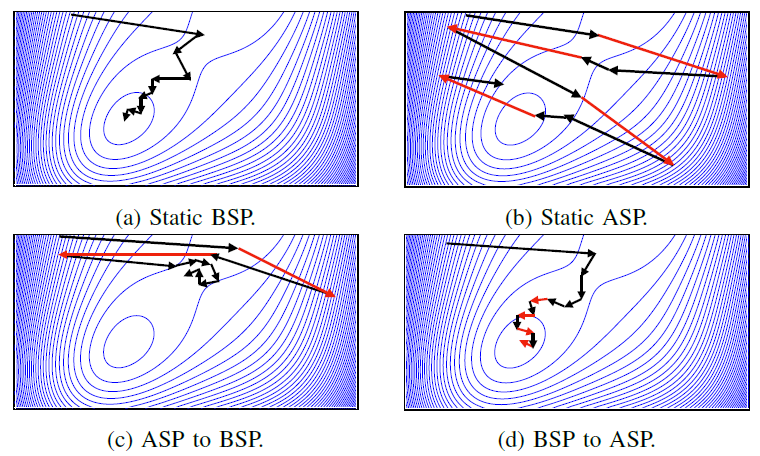
\includegraphics[scale=0.6]{P27.png}
		\caption{ترکیبات مختلف \lr{BSP} و \lr{ASP} بر روی یک تابع هزینه ساده \cite{Syncswitch2021}}
		\label{p27}
	\end{center}
\end{figure}

در الگوریتم گرادیان کاهشی تصادفی دسته‌ای \lr{(Minibatch SGD)} هر گره گرادیان را با استفاده از داده‌های محلی خودش محاسبه کرده و سپس گره‌ها گرادیان‌های محلی‌شان را میانگین می‌گیرند و از گرادیان حاصل برای به‌روزرسانی نهایی استفاده می‌شود. الگوریتم گرادیان کاهشی تصادفی محلی (\lr{Local SGD}) به عنوان بهبودی بر الگوریتم دسته‌ای پیشنهاد شده است. در این الگوریتم در هر دور هر گره \lr{K} گام از \lr{SGD} را بر روی هدف محلی و داده‌های خودش اجرا می‌کند. در نهایت نتایج به‌روزرسانی گره‌ها به عنوان نتیجه نهایی آن دور میانگین‌گیری می‌شود. در محیط‌های همکن و نزدیک به همگن نسخه محلی بر دسته‌ای غلبه می‌کند. در \cite{Minibatch2020} کارایی این دو نسخه در محیط‌های ناهمگن مورد بررسی قرار گرفته است. آنها نشان دادند که با تغییر تنظیمات از همگن به ناهمگن، کارایی نسخه محلی به طور قابل توجهی کاهش پیدا می‌کند. هر دوی این الگوریتم‌ها متمرکز می‌باشند.

همان‌طور که ذکر شد، الگوریتم گرادیان کاهشی تصادفی محلی برای همه سناریوها قابل اجرا نیست. گره‌ها ممکن است از نظر قابلیت‌های محاسباتی ناهمگن باشند و زمان مورد نیاز برای یادگیری محلی گره‌ها یکسان نیست. به همین دلیل یادگیری کاملا همگام گره‌ها ممکن است پرهزینه یا حتی غیرممکن باشد. اکثریت قریب به اتفاق کارهای ارائه شده یک مدل همگام استفاده می‌کنند که در آن همه گره‌ها قبل از ارسال به‌روزرسانی‌هایشان به سرور مرکزی، با تعداد تکرار یکسانی آموزش می‌بینند. همچنین در بیشتر کارهای انجام‌شده مدل ارتباطی \lr{Hub-and-Spoke} فرض می‌شود، اما این مدل بسیاری از حالت‌های دنیای واقعی را نشان نمی‌دهد. به عنوان مثال، دستگاه‌های موجود در یک شبکه اقتضایی متحرک به دلیل محدودیت‌های شبکه یا محدوده ارتباطی، ممکن است همه نتوانند در یک گام با سرور مرکزی ارتباط برقرار کنند. در چنین حالتی، یک مدل شبکه ارتباطی چند سطحی مناسب است. 

در \cite{zhou2019} الگوریتمی به نام \lr{SGD} محلی سلسله مراتبی \lr{ (HL-SGD)} برای یادگیری مدل در یک شبکه سلسله مراتبی با توپولوژی \lr{Hub-and-Spoke} پیشنهاد شده است و همه گره‌های شبکه همگن فرض شده‌اند. تحلیل خطا همگرایی و زمان همگرایی الگوریتم \lr{HL-SGD } در مقاله‌های \cite{Liu2020, Abad2020} برای یادگیری فدرالی \footnote{\lr{Federated Learning}} بحث شده است. الگوریتم \lr{SGD} محلی چندسطحی \lr{MLL-SGD} \cite{MLL2020} یک الگوریتم یادگیری توزیع‌شده برای شبکه‌های سلسله مراتبی با گره‌های ناهمگن است. در این الگوریتم، ساختار شبکه به صورت دو سطحی در نظر گرفته شده است. سطح پایین‌تر شامل مجموعه‌ای از شبکه‌های فرعی \lr{Hub-and-Spoke } است که هر کدام دارای یک سرور هاب و مجموعه‌ای از گره‌ها است. شبکه سطح بالا شامل یک شبکه هاب متصل که توسط آن هاب‌ها با هم ارتباط برقرار می‌کنند. هر شبکه فرعی چند دور \lr{SGD} محلی را اجرا می‌کند. بعد از یک دوره آموزش محلی گره‌ها، در مرکز شبکه فرعی میانگین‌گیری مدل انجام می‌شود. به طور دوره‌ای، هاب‌ها مدل‌های خود را با همسایگان در شبکه هاب میانگین‌گیری می‌کنند. در \cite{Fed6} پیشنهاد شده که از الگوریتم‌های بهینه‌سازی‌ غیر از \lr{SGD} در گره‌ها یا از یک قانون به‌روزرسانی جایگزین در سرور مرکزی استفاده شود. 

مکانیزم‌های کنترل مانع در الگوریتم‌های یادگیری تکراری نقش بسیار حیاتی را ایفا می‌کنند. در اغلب محاسبات داده-موازی، پارامترهای مدل اشتراکی براساس به‌روزرسانی‌های جداگانه از هر قطعه داده به‌روز می‌شوند. به عبارت دیگر، به‌روزرسانی‌های تجمیع‌شده برای به‌روزرسانی مدل استفاده می‌شوند. به‌روزرسانی‌های همگام نشده باعث ایجاد خطا و نویز در مدل نهایی خواهند شد. 

در یک محیط بسیار نامطمئن، لینک‌ها ممکن است خراب شوند و پهنای باند ناهمگن است؛ همچنین گره‌ها ثابت نیستند، می‌توانند در هر زمان به سیستم بپیوندند و یا از آن خارج شوند. بنابراین، در چنین محیطی با تضمین اینکه اکثر سیستم‌ها دارای مرز همگام‌شده هستند، می‌توان این تأثیرات را به حداقل رساند. میزان همگام‌سازی یک مانع نشان‌دهنده‌ی مبادله بین دقت (در هر تکرار) و کارایی (سرعت همگرایی) یک الگوریتم یادگیری تکراری است. با توجه به مزایا و معایب هر مکانیزم همگام‌سازی، \lr{BSP} قطعی است و می‌تواند به همان طراحی الگوریتم یادگیری ماشین منجر شود. مکانیزم‌های قطعی نظارت و کنترل همگام‌سازی مانع در یک محیط بسیار پویا ممکن است مناسب نباشند. در مقاله \cite{wang2017} یک تکنیک کنترل مانع احتمالی به نام \lr{PSP}\footnote{\lr{Probabilistic Synchronous Parallel}} بر اساس یک نمونه‌گیری اولیه ارائه شده است که در مقایسه با سه تکنیک کنترل مانع رایج در یک سیستم بسیار پویا و خیلی بزرگ به طور موثر سرعت همگرایی و مقیاس‌پذیری الگوریتم گرادیان کاهشی تصادفی را بهبود می‌بخشد. همگام‌سازی مانعی در تکنیک \lr{PSP} به روش احتمالی کنترل می‌شود، یعنی با نمونه‌برداری از گره‌های شرکت‌کننده در یادگیری درصدی از گره‌های سیستم که مرحله فعلی را به پایان رسانده‌اند را تخمین می‌زند. ایده اصلی مکانیزم \lr{PSP} این است که ما نیاز داریم که فقط بخشی از گره‌ها نه همه آنها، در پروسه همگام‌سازی قرار بگیرند. روش‌های موجود کنترل همگام‌سازی مانع و سازگاری مدل را تجمیع می‌کنند، درحالیکه \lr{PSP} کنترل همگام‌سازی مانع را از سازگاری مدل جدا می‌کند. 

در یادگیری فدرالی، گره‌های توزیع‌شده و ناهمگن برای یادگیری پارامترهای مدل با یکدیگر همکاری می‌کنند. با این‌حال، در حالی که مزایایی مانند حفظ حریم خصوصی با طراحی و کاهش تأخیر ایجاد می‌کند، شبکه ناهمگن چالش‌هایی را برای روش‌های همگام‌سازی یا روش‌های کنترل موانع، در مورد پیشرفت سیستم و همگرایی مدل و غیره ایجاد می‌کند. در \cite{Zhao2021} از مکانیزم \lr{PSP} برای یادگیری فدرال استفاده شده است و آنها پیشنهاد دادند که می‌توان مکانیزم‌های موجود، به ویژه \lr{BSP} و \lr{SSP}، را برای ایجاد مکانیزم‌های کنترل مانع کاملاً توزیع‌شده و مقیاس‌پذیرتر ترکیب کرد. این کار سبب می‌شود که با بزرگتر شدن سیستم به منظور جلوگیری از خفه شدن سرور و عدم ایجاد تنگنا، ارتباطات بین گره‌ها و سرور کاهش یابد. در شکل \ref{p28} مکانیزم احتمالی \lr{PSP} با \lr{BSP} ترکیب شده است و در نمونه‌برداری اولیه انجام شده از گره‌های موجود در سیستم، مکانیزم کنترل مانع \lr{BSP} اجرا شده است. 
\begin{figure}
	\begin{center}
		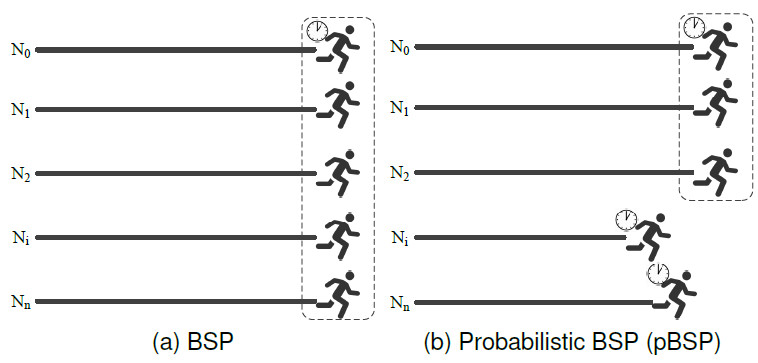
\includegraphics[scale=0.6]{P28.png}
		\caption{ترکیب \lr{PSP} با مکانیزم کنترل مانع \lr{BSP} \cite{wang2017}}
		\label{p28}
	\end{center}
\end{figure}

مقاله \cite{Fed9_2021} به بررسی فرصت‌های جدید یادگیری توزیع‌شده فدرالی برای سیستم‌های صنعتی شبکه‌ای نسل بعدی پرداخته است و مسائلی با تمرکز بر رانندگی مشارکتی در وسایل نقلیه خودکار متصل و روباتیک مشارکتی در تولید هوشمند مورد بحث قرار گرفته‌اند. راه‌حل‌های غیرمتمرکز پتانسیل بالایی برای نسل پنجم (\lr{5G}) صنعتی دارند. در مقاله \cite{Fed7_2021} رویکرد یادگیری توزیع‌شده غیرمتمرکزی مبتنی بر تبادل متقابل اجماع برای وسایل نقلیه خودکار متصل به منظور دسته‌بندی عوامل جاده ارائه شده است. عوامل جاده مانند عابران پیاده، مخروط‌های ترافیکی، موانع، دوچرخه‌ها، اتومبیل‌ها و اتوبوس‌ها  که هر وسیله نقلیه آن‌ها را با اسکن محیط از طریق خود توسط سنسور شناسایی می‌کند که در آن هدف وسایل نقلیه یادگیری مشارکتی یک مدل یادگیری عمیق مبتنی بر \lr{PointNet} برای استنباط نوع واقعی عوامل جاده است. 

برای رفع نیاز به همگام‌سازی دقیق در مکانیزم \lr{BSP} و کاهش زمان انتظار گره‌های سریع در مقاله \cite{zhao2020elastic} یک روش همگام‌سازی الاستیک یا قابل ارتجاع به نام \lr{ElasticBSP} پیشنهاد شده است. این روش همکام‌سازی مبتنی بر یک الگوریتم به نام \lr{ZipLine} است که زمان اجرای همگام‌سازی را تخمین می‌زند. در مرحله اول برای هر گره نقاط پایانی در تکرارهای آینده در زمان اجرا تخمین زده می‌شوند و در مرحله دوم یک الگوریتم تک-گذر بر روی نقاط پایانی تخمین زده شده‌ی همه گره‌ها اجرا می‌شود تا یک نقطه زمانی بهینه در تکرار بعدی برای همگام‌سازی به صورت سریع محاسبه گردد. 

هدف این روش تسهیل شرایط همگام‌سازی دقیق مکانیزم \lr{BSP} برای کاهش زمان انتظار گره‌ها و در نتیجه افزایش توان تکرارها، و در عین حال محدود کردن گرادیان‌های قدیمی و مقادیر قدیمی آنها در روند همگرایی الگوریتم گرادیان کاهشی تصادفی تکراری است. همچنین در مقایسه با مکانیزم \lr{SSP}، مدل پیشنهادی ظرفیت محاسباتی گره‌ها را در نظر می‌گیرد. بنابراین انعطاف‌پذیری و سازگاری بیشتری را در طول مرحله یادگیری بدون کاهش دقت مدل آموزشی، ارائه می‌دهد. 

در روش \lr{ElasticBSP}، زمان اعمال مانع همگام‌سازی متفاوت است و هر ابرگام تعداد متفاوتی از تکرارها را برای هر گره مجاز می‌کند. این مقادیر در زمان اجرا توسط الگوریتم \lr{ZipLine} تعیین می‌شوند که حداقل زمان انتظار کلی همه گره‌ها را به دست می‌آورد. شکل \ref{p2930} به خوبی تفاوت زمان اجرای ابرگام‌ها در \lr{BSP} و \lr{ElasticBSP}  در یک شبکه با 4 گره را نشان می‌دهد. در هر ابرگام قسمت رنگی هر گره زمان محاسبات و قسمت سفید رنگ زمان ارتباطات را بیان می‌کنند.
%\iffalse
\begin{figure}
	\centering
	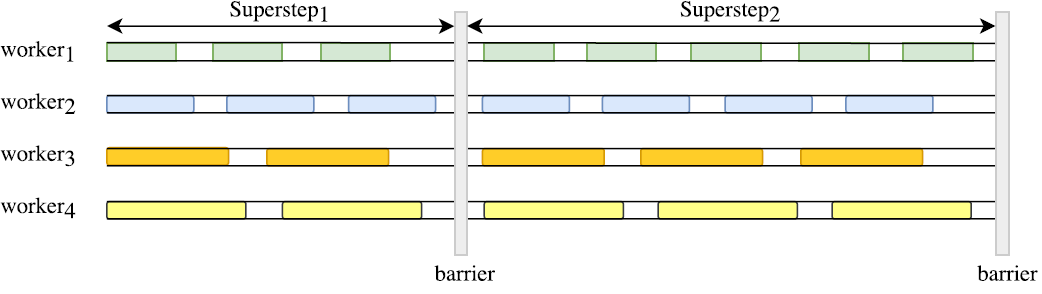
\includegraphics[width=\textwidth]{Pic29.png}
	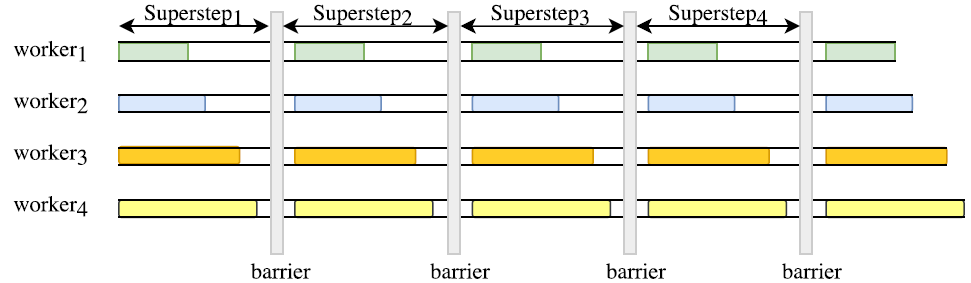
\includegraphics[width=\textwidth]{Pic30.png}
	\caption{تفاوت زمان اجرای ابرگام‌ها در \lr{BSP} و \lr{ElasticBSP} \cite{Zip2021}}
	\label{p2930}
\end{figure}







\subsection{الگوریتم‌های یادگیری تطبیقی انتشاری}\label{DfsnAlg}


الگوریتم‌های یادگیری تطبیقی انتشاری بر اساس پردازش داده و همکاری‌ها بین گره‌ها پایه‌ریزی شده‌اند و هر گره با استفاده از داده‌هایی که در اختیارش می‌باشد، تخمینی از پارامترهای مجهول ارائه می‌دهد و می‌تواند با توجه به توپولوژی شبکه با همسایه‌هایش تعامل داشته باشد و از آن‌ها اطلاعات دریافت کند و به آن‌ها نیز اطلاعاتی ارسال نماید. بنابراین، پردازش انجام شده مبتنی‌بر داده‌های محلی هر گره و اطلاعات دریافتی از همسایه‌هایش می‌باشد. بر خلاف روش تخمین پارامتر متمرکز، در این روش هیچ گره مرکزی وجود ندارد و قادر است سربار ارتباطی و پردازشی را کاهش دهد. اکثر کارهای ارائه‌شده در زمینه برآورد پارامتر از طریق شبکه‌های تطبیقی توزیع‌شده به صورت یک مساله کمینه‌سازی اجماع توابع هزینه هر گره مطرح می‌شوند. گره‌ها با توابع زیان مجزا اما هم مدل در جستجوی یک هدف مشترک هستند و نیاز به همگرا شدن به سمت یک پارامتر مشترک دارند. این مسائل تک‌وظیفه‌ای نامیده می‌شوند. 

در شکل \ref{p11} دسته‌بندی الگوریتم‌های یادگیری تطبیقی انتشار برای مقابله با چالش‌های موجود در شبکه‌های تطبیقی توزیع‌شده نشان داده شده است. این دسته‌بندی براساس سه دیدگاه انجام شده است: الف) تک وظیفه‌ای و چندوظیفه‌ای ب) روش‌های همگام و غیرهمگام ج) تابع هدف. جزییات این الگوریتم‌ها در ادامه همین بخش بیان شده است. در دسته‌بندی انجام شده شکل \ref{p11}، الگوریتم‌های یادگیری انتشاری پیشنهادی در این رساله به منظور مشخص شدن جایگاه شان نیز آورده شده‌اند. 

\begin{figure}
	\begin{center}
		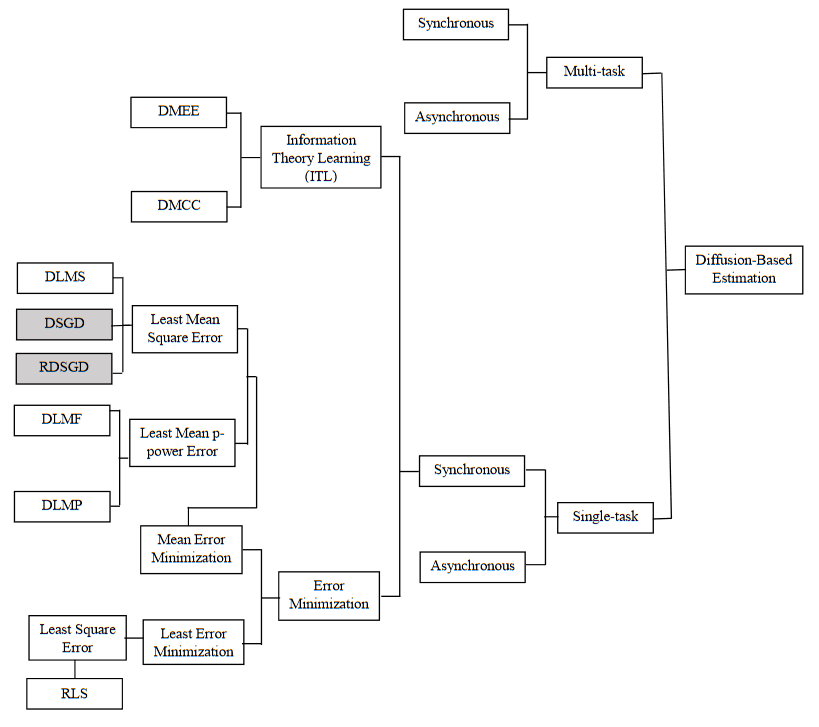
\includegraphics[scale=1.2]{CatDiffusion__.PNG}
		\caption{دسته‌بندی الگوریتم‌های یادگیری تطبیقی انتشار}
		\label{p11}
	\end{center}
\end{figure}

در مقاله \cite{Lop2008} الگوریتم \lr{DLMS} که مبتنی بر روش همکاری انتشار می‌باشد از استراتژی تطبیق سپس ترکیب \lr{ATC }\footnote{\lr{Adapt Then Combine (ATC)}} يا تركيب سپس تطبيق  \lr{CTA} \footnote{\lr{Combine Then Adapt (CTA)}} برای حل رابطه بهینه‌سازی \ref{e1} استفاده می‌کند. روابط زیر فرم به‌روزرسانی کلی \lr{ATC} برای هر گره $k$ را نشان می‌دهند.

\begin{equation}\label{ATC1}
	\begin{cases}
		\psi_{k}(i+1)=w_{k}(i)-\mu_k\sum_{l\in N_k}c_{lk}\nabla_{w}{J_l(w_{k}(l))}\quad\text{(\lr{Adapt})}\\
		w_{k}(i+1)=\sum_{l\in N_k}a_{lk}\psi_{l}(i+1) \quad  \text{(\lr{Combine})}
	\end{cases}
\end{equation}

همچنين روابط فرم به‌روزرسانی کلی \lr{CTA} برای هر گره $k$ به صورت زير بيان مي‌شوند:
\begin{equation}\label{CTA1}
	\begin{cases}
		\psi_{k}(i)=\sum_{l\in N_k}a_{lk}w_{l}(i)\quad  \text{(\lr{Combine})}\\
		w_{k}(i+1)=\psi_{k}(i)-\mu_k\sum_{l\in N_k}c_{lk} \nabla_{w}{J_l(\psi_{k}(i))}\quad\text{(\lr{Adapt})}
	\end{cases}
\end{equation}
که ${J_l(\psi_{k}(i))}$ تخمین بردار گرادیان گره $l$ می‌باشد و $\mu_k$ ضریب همگرایی و $c_{lk}$ و $a_{lk}$ ضرایب غیرمنفی هستند که براساس شرایط زیر تعریف می‌گردند:
\begin{equation}\label{e8}
	a_{lk}>=0,\qquad\sum_{l\in N_k}a_{lk}=1, \qquad and\quad a_{lk}=0 \quad if \quad  l\notin N_k
\end{equation}

\begin{equation}\label{e9}
	c_{kl}>=0, \qquad \sum_{l\in N_k}c_{kl}=1,\qquad and\quad c_{kl}=0\quad if \quad l\notin N_k 
\end{equation}

طبق شرط‌های ذکر شده برای ضرایب $c_{lk} $ و $a_{lk}$ با جمع‌آوری آنها در یک ماتریس  \lr{N*N} دو ماتریس ترکیبی وزن‌دار $A=[a_{lk}]$ و $C=[c_{lk}] $ به صورت $1C=1$ و $1A^T=1$ تعریف می‌شوند. روش‌های متعددی برای انتخاب ضرایب وزن همسایگی $a_{lk}$ بین دو گره در شبکه ارائه شده است. یکی از ساده‌ترین روش‌ها براساس تعداد گره‌های همسایه است که به صورت زیر تعریف می‌شود:

\begin{equation}\label{e10}
	a_{lk}=
	\begin{cases}
		\frac{1}{|N_k|} \quad  l\in N_k\\
		0 \quad l\notin N_k
	\end{cases}
\end{equation}
در شکل \ref{p7} روش‌های دیگری که برای انتخاب ضرایب $a_{kl} $ استفاده می‌شوند، ذکر شده است.
\begin{figure}
	\begin{center}
		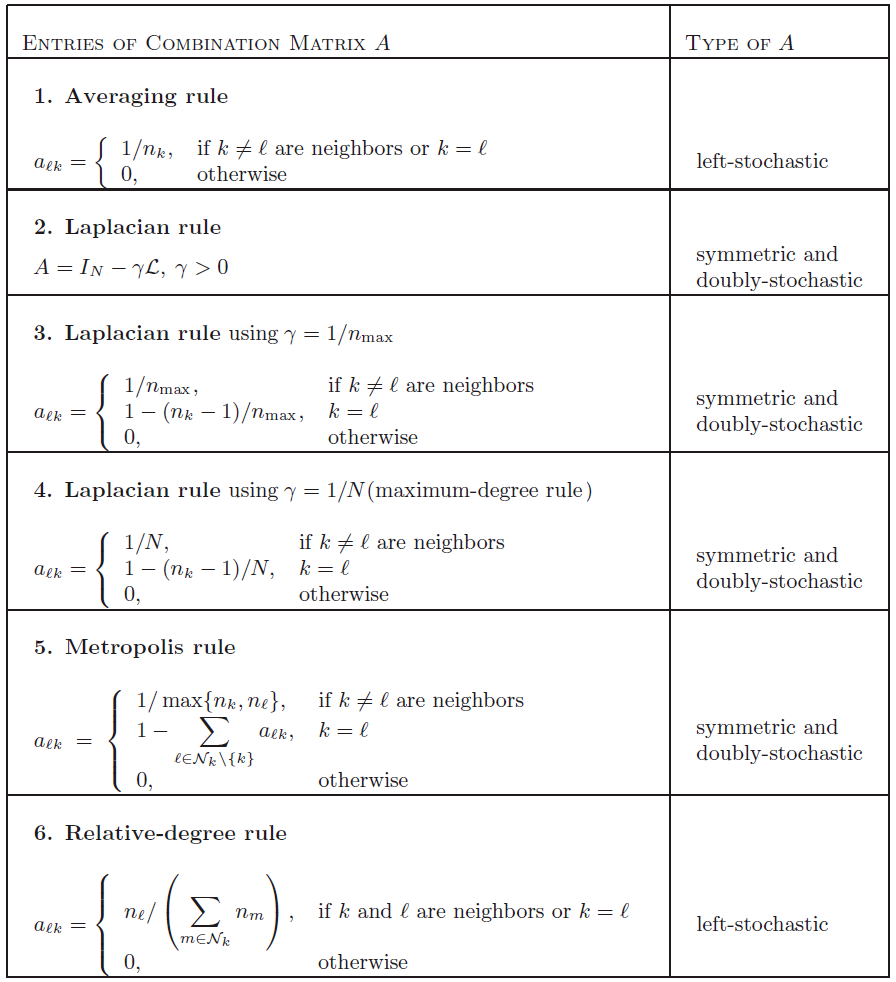
\includegraphics[scale=0.6]{Pic7.png}
		\caption{روش‌های مختلف تعریف ضرایب وزن همسایگی  \cite{SayedBook}}
		\label{p7}
	\end{center}
\end{figure}

شکل \ref{p8} استراتژی \lr{ATC} را در شبکه‌های تطبیقی توزیع‌شده با روش انتشار نشان می‌دهد. همان طور که دیده می‌شود، هر گره $k$ ابتدا با استفاده از فیلتر وفقی خود به‌روزرسانی بردار پارامتر میانی را انجام می‌دهد و سپس بردارهای پارامتر میانی همسایگان را ترکیب می‌نماید.
\begin{figure}
	\begin{center}
		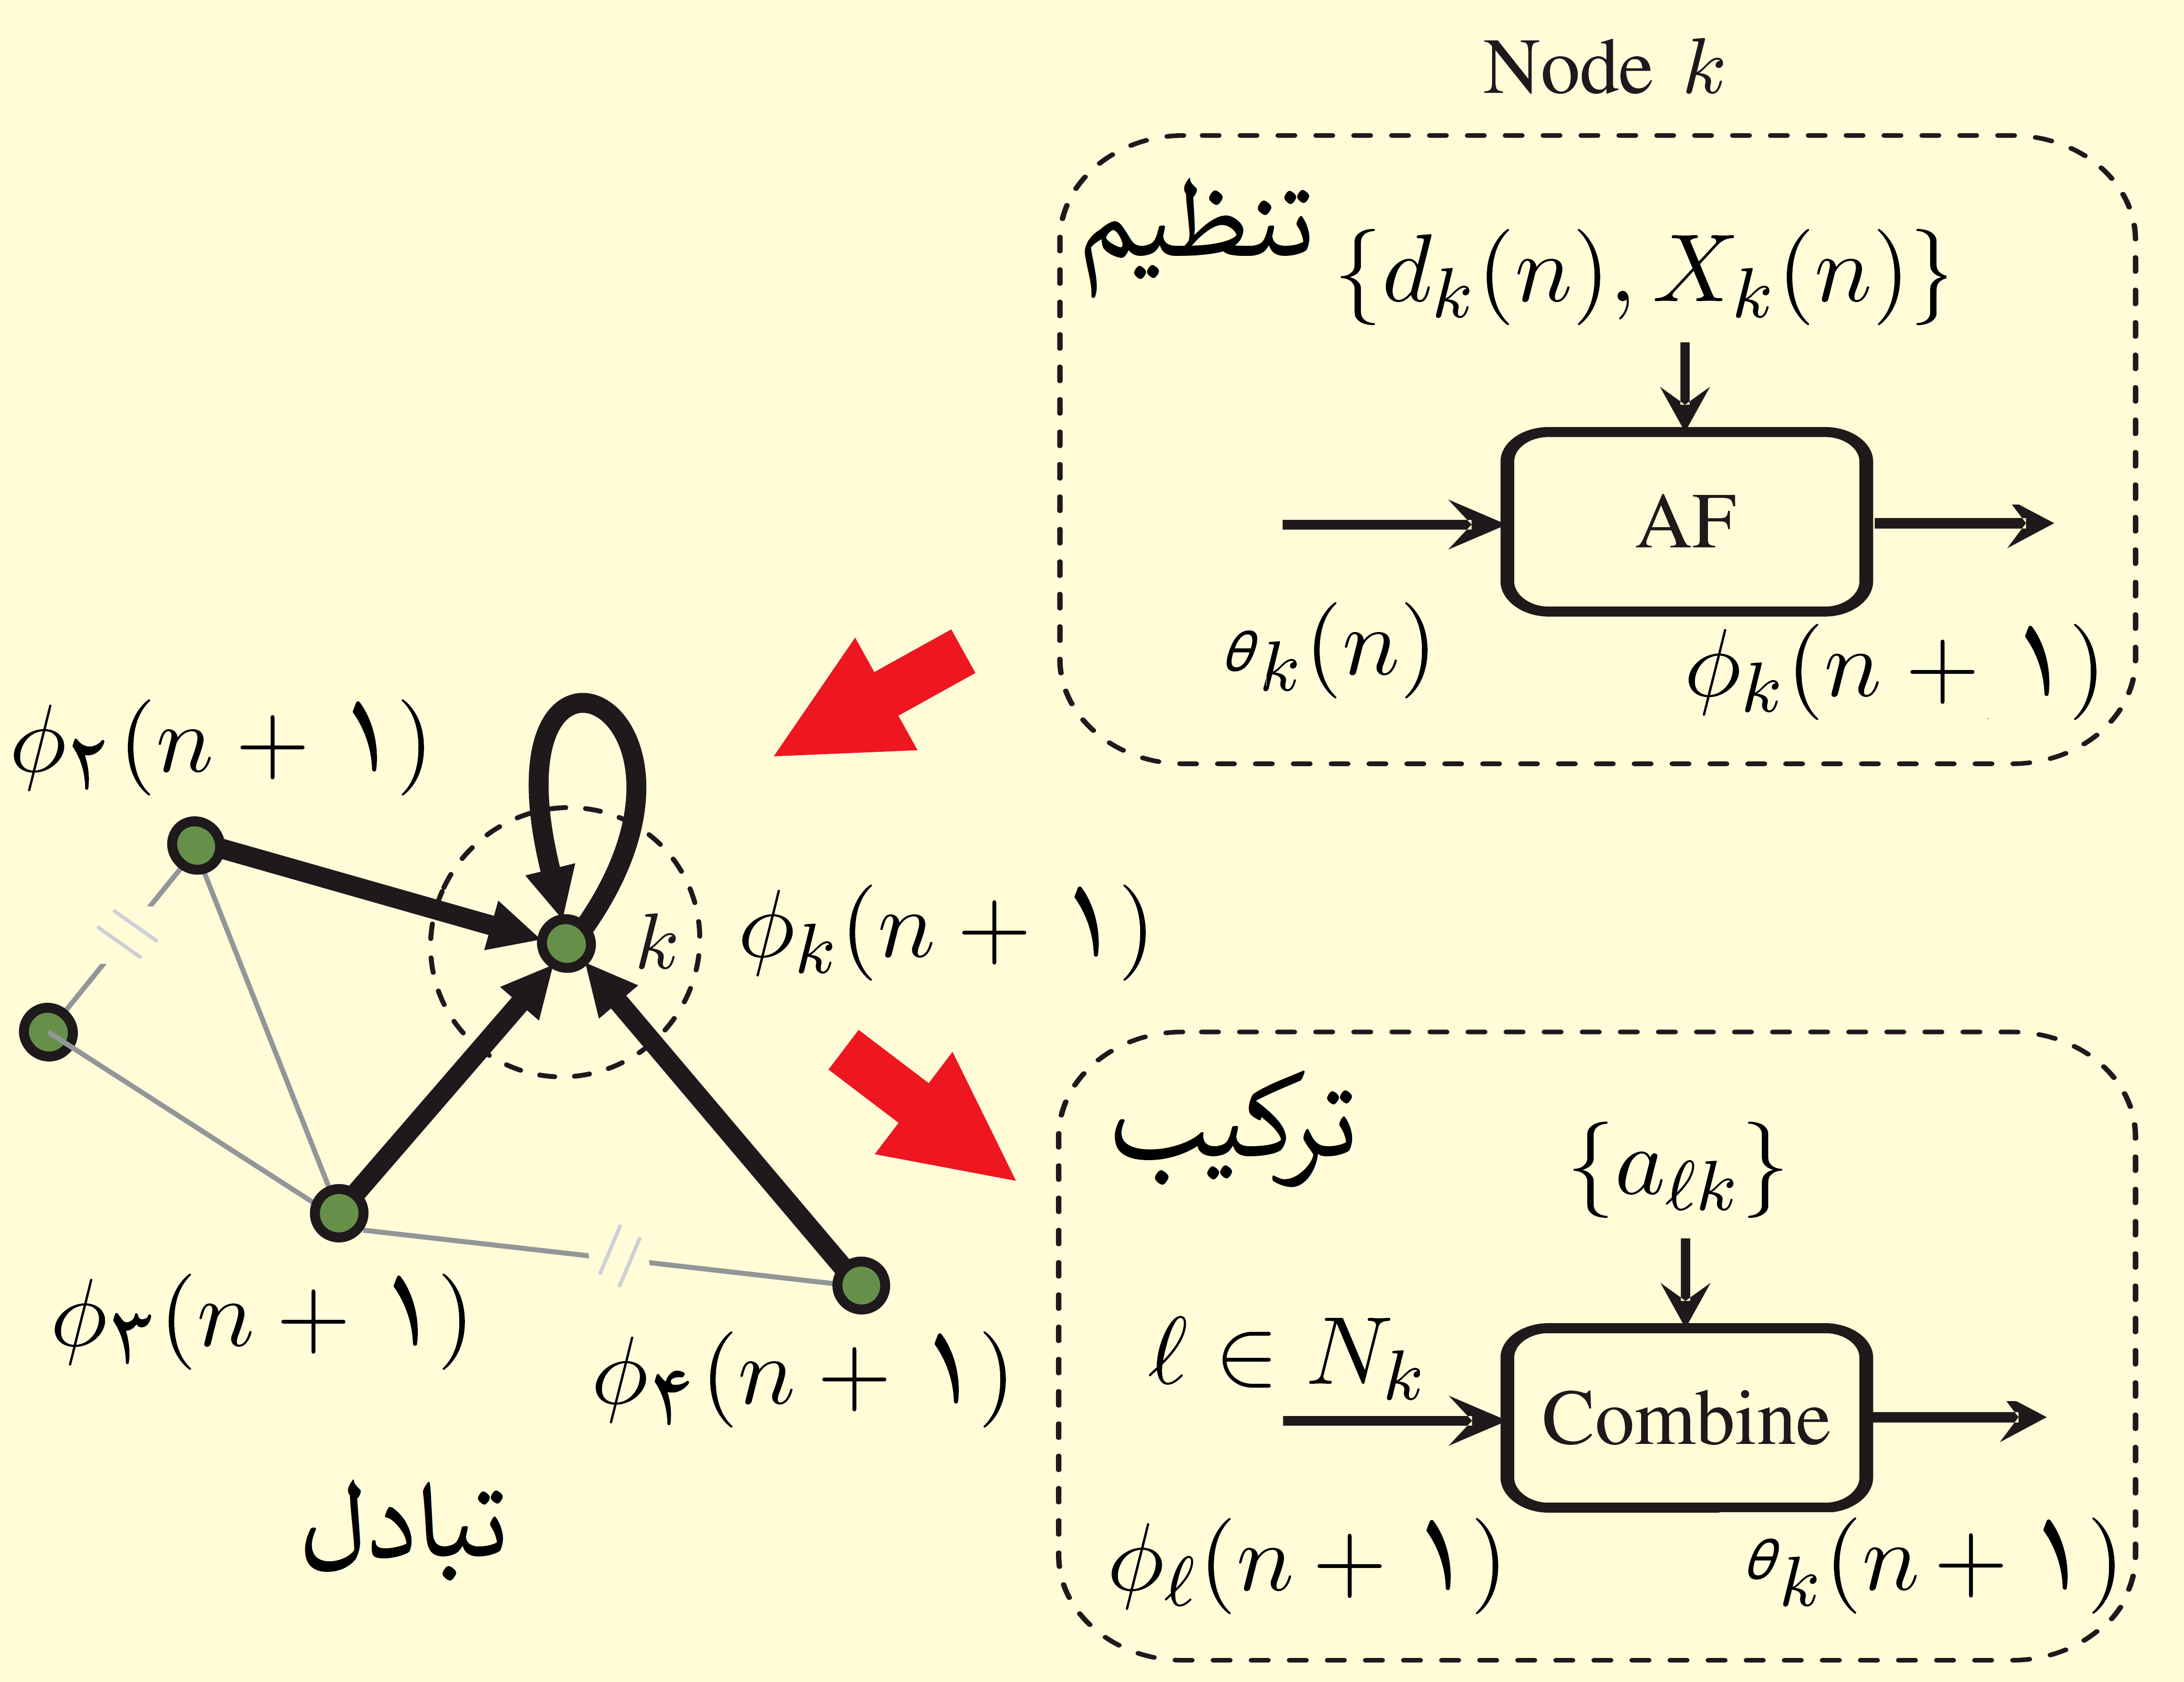
\includegraphics[scale=0.07]{Pic8.JPG}
		\caption{استراتژی \lr{ATC} در شبکه‌ تطبیقی انتشاری  \cite{SayedBook}}
		\label{p8}
	\end{center}
\end{figure}
در استراتژی تركيب سپس تطبيق يا همان \lr{CTA} ابتدا تخمين مياني با تركيب تخمين‌هاي محلي گره‌هاي همسايه محاسبه مي‌گردد. سپس با استفاده‌ از داده‌هاي محلي گره $k$ و تخمين مياني بدست آمده از گام اول، عمليات تطبيق انجام مي‌شود. شکل \ref{p9} استراتژی \lr{CTA} را در شبکه‌های تطبیقی توزیع‌شده با روش انتشار نشان می‌دهد.

\begin{figure}
	\begin{center}
		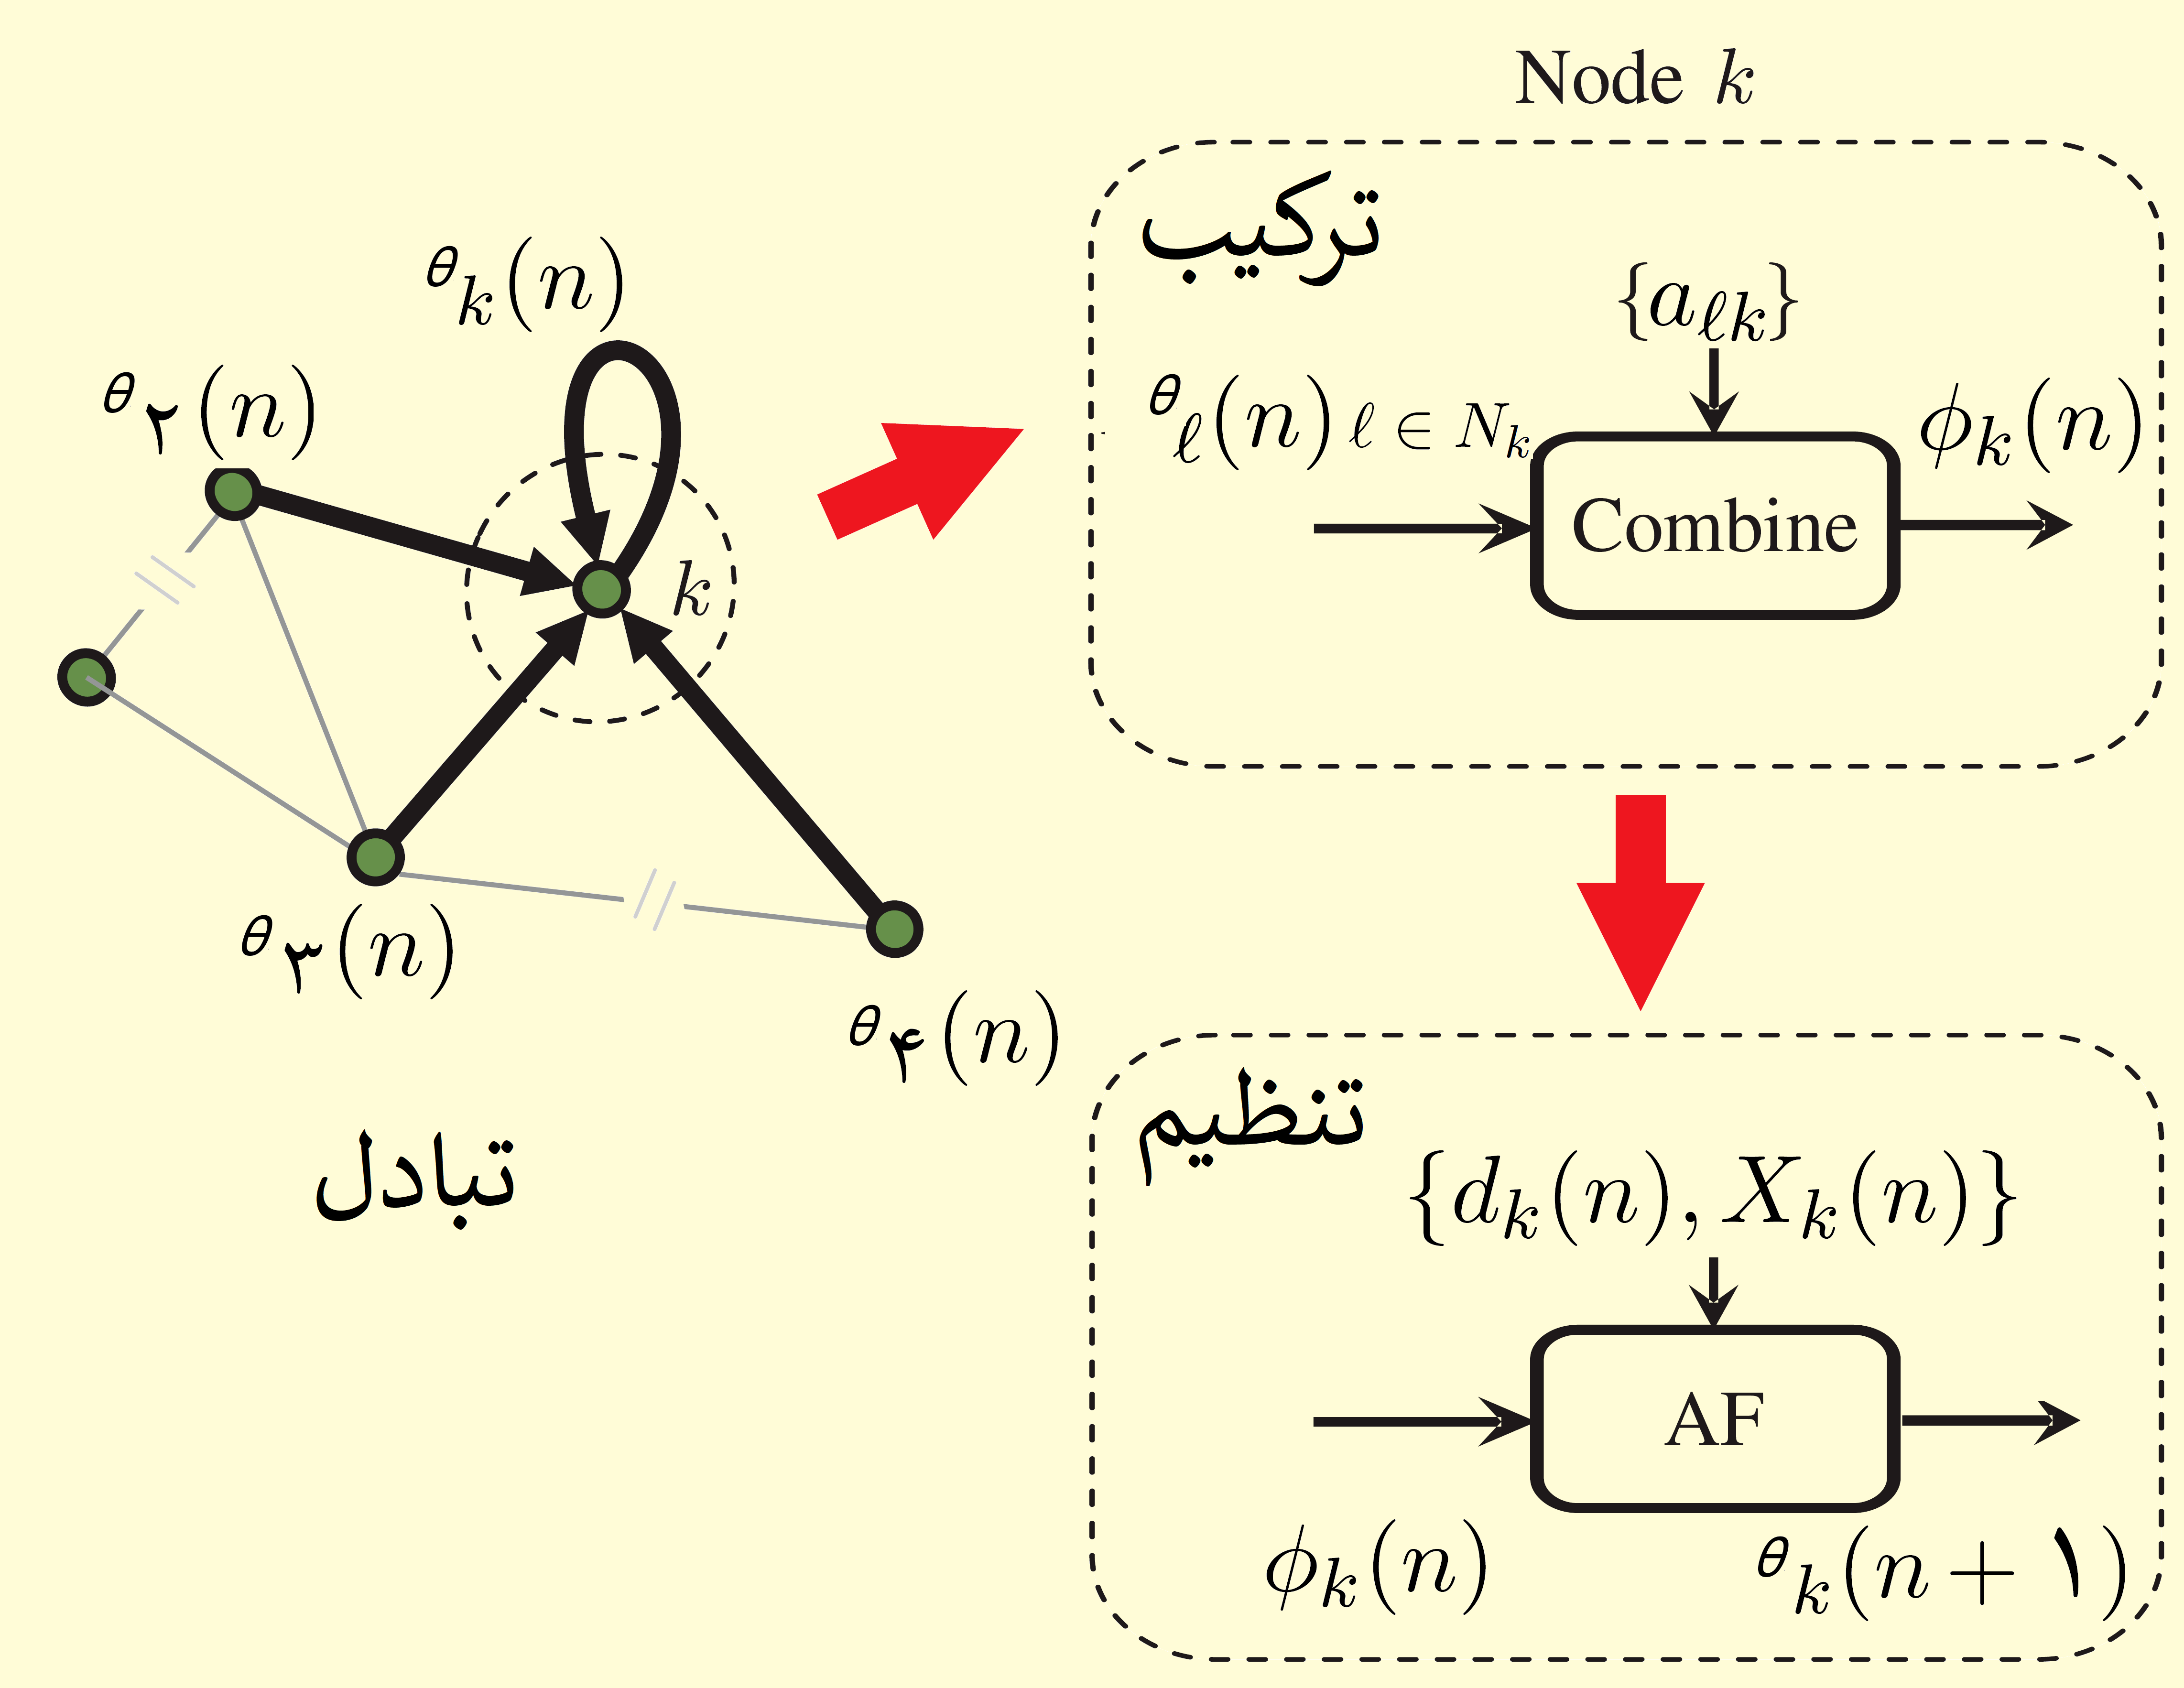
\includegraphics[scale=0.07]{Pic9.JPG}
		\caption{استراتژی \lr{CTA} در شبکه‌ تطبیقی انتشاری  \cite{SayedBook}}
		\label{p9}
	\end{center}
\end{figure}


سایر روش‌های ارائه شده برای حل \lr{DLMS} از جمله استراتژی \lr{ATC} بدون تبادل اطلاعات بین گره‌های همسایه در مرحله تطبیق، استراتژی ترکیب سپس تطبیق \lr{CTA} بدون تبادل اطلاعات در شکل \ref{p10} لیست شده‌اند \cite{Cat20081}. 

\begin{figure}
	\begin{center}
		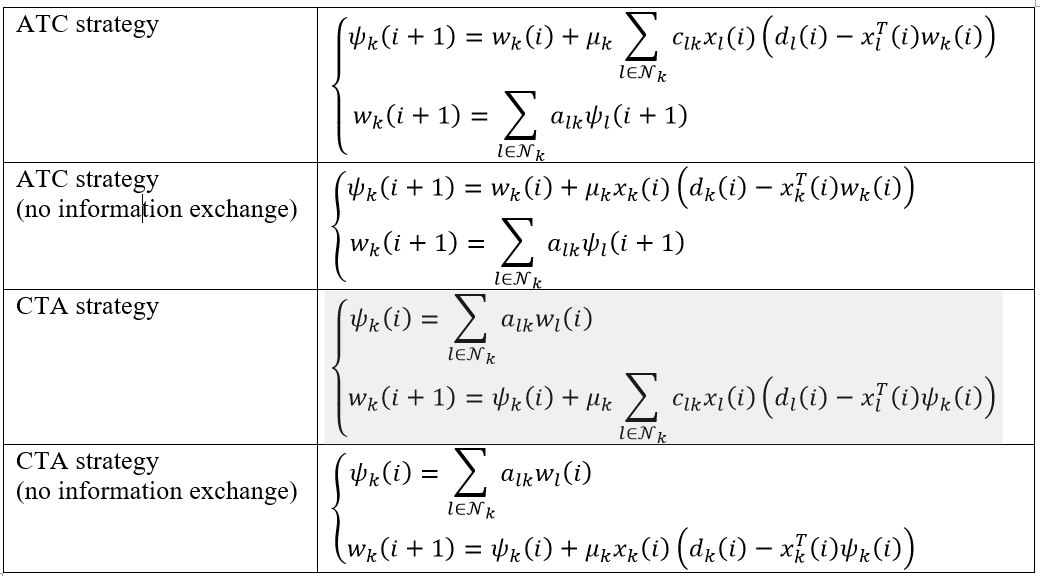
\includegraphics[scale=0.8]{Pic10.JPG}
		\caption{: روش‌های مختلف حل \lr{DLMS}   \cite{Cat20081}}
		\label{p10}
	\end{center}
\end{figure}

در مقاله \cite{Cat20082} با استفاده از فيلتر \lr{RLS} الگوریتم یادگیری توزیع‌شده انتشاري به نام \lr{DRLS} ارائه شده است. با فرض مدل شدن ورودي‌هاي فيلتر با رگرسيون خطي بيان‌شده در رابطه \ref{e6} و تعريف ماتريس‌هاي \lr{A} و \lr{C} همانند الگوریتم \lr{DLMS}، مساله بهينه‌سازي زير با ترم تنظيم $\delta$  و ضريب فراموشي $\lambda$\footnote{\lr{Forgetting factor}}  به منظور تخمين بردار پارامتر $w^o$ استفاده مي‌شود:

\begin{equation}\label{e13}
	\min_w \lambda^{i+1}\delta ||w||^2 +\sum_{l=0}^{i}\lambda^{i-j}(\sum_{k=1}^{N}(d_k(i)-u_k^T(i)w)^2)
\end{equation}

كه $\delta>0$ و  ضریب فراموشي $0\le\lambda\le1$ است. حل مساله بهينه‌سازي بيان شده در رابطه \ref{e1} بر اساس استراتژي \lr{ATC} در ادامه آورده شده است. براي هر گره $k$، مقادير اوليه زير در نظر گرفته مي‌شود:

\begin{equation}\label{e14}
	\begin{cases}
		w_{k,-1}=0,\quad P_{k,-1}=\delta^{-1}I_M\\
		\psi_{k,i}=w_{k,i-1}\\
		P_{k,i}=\lambda^{-1}P_{k,i-1}
	\end{cases}
\end{equation}

براي هر گره $k$ روابط گام تطبيق با تكرار بر روي همه همسايگان $l\in N_k$ و گام تركيب اين رويكرد به صورت زير بيان مي‌شوند:

\begin{equation}\label{e141}
	\begin{cases}
		\begin{cases}
			\psi_{k,i}=\psi_{k,i}+\frac{c_{lk}P_{k,i}u_{l,i}^T}{1+c_{lk}u_{l,i}P_{k,i}u_{l,i}^T}\left[d_{l,i}-u_{l,i}\psi_{k,i}\right]\\
			P_{k,i}=P_{k,i}-\frac{c_{lk}P_{k,i}u_{l,i}^T u_{l,i}P_{k,i}}{1+c_{lk}u_{l,i}P_{k,i}u_{l,i}^T}
		\end{cases}\quad  \text{(\lr{Adapt})}\\
		w_{k,i}=\sum_{l\in N_k}a_{lk}\psi_{l,i}\quad  \text{(\lr{Combine})}
	\end{cases}
\end{equation}

در مقاله\cite{Jung2013} روشي براي جبران باياس بر اساس نسخه نرمال \lr{LMS} ارائه شده است تا بتواند اثر منفي نويز ورودي را كاهش دهد. براي حذف باياس نويز ورودي از معياري استفاده شده كه نيازمند تخمين واريانس نويز ورودي است. اما زمانيكه نويز ضربه‌اي باشد، تخمين واريانس نويز چندان موفقيت‌آميز نمي‌باشد. بنابراين براي حل اين مشكل، تخمين واريانس نويز ورودي زمان رخ دادن نويز ضربه‌اي به‌روز خواهد شد. اگر خطا از يك حد مشخصي بيشتر شود، واريانس نويز ورودي مجدد تخمين‌زده مي‌شود و سپس مقدار بردار پارامتر به‌روزرساني مي‌شود. در مقاله \cite{Zheng2017} از الگوريتم حداقل توان چهارم خطا براي بدست آوردن تخميني بدون باياس استفاده شده است. 

\begin{figure}
	\begin{center}
		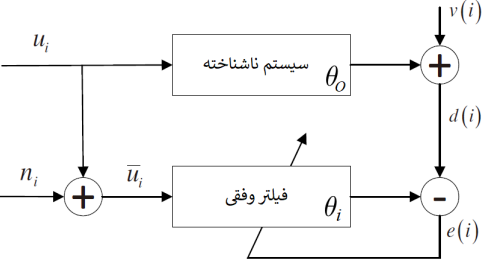
\includegraphics[scale=0.9]{Filter.png}
		\caption{فیلتر تطبيقي با نويز ورودي}
		\label{filter}
	\end{center}
\end{figure}

در شبكه‌هاي تطبيقي توزيع‌شده براي مقابله با مساله نويز ورودي روش‌هايي مختلفی ارائه شده است. شكل \ref{p24} اين مساله را در شبكه‌هاي تطبيقي نشان مي‌دهد. در مقاله \cite{Abdolee2016} روشي بر اساس تخمين واريانس نويز پيشنهاد داده‌اند كه تابع هدف هر گره \lr{k} به صورت زير تعريف مي‌شود:
\begin{equation}\label{e142}
	J_k(w)=E\lvert\lvert d_k(i)-u_{k,i}w\rvert\rvert^2-\sigma^2_{k,i}\lvert\lvert w \rvert\rvert^2
\end{equation}


كه $\sigma_{k,i}^2$ واريانس نويز ورودي در گره $k$ام شبكه است. از الگوريتم انتشار براي حل اين مساله بهينه‌سازي استفاده مي‌شود و روابط به‌روزرساني به‌دست مي‌آيد. اين روش نيازمند تخمين واريانس نويز ورودي است. برخي از كارهاي ارائه شده از توابع زيان پايدارتري براي مقابله با نويز‌هاي ورودي كمك مي‌گيرند. 

\begin{figure}
	\begin{center}
		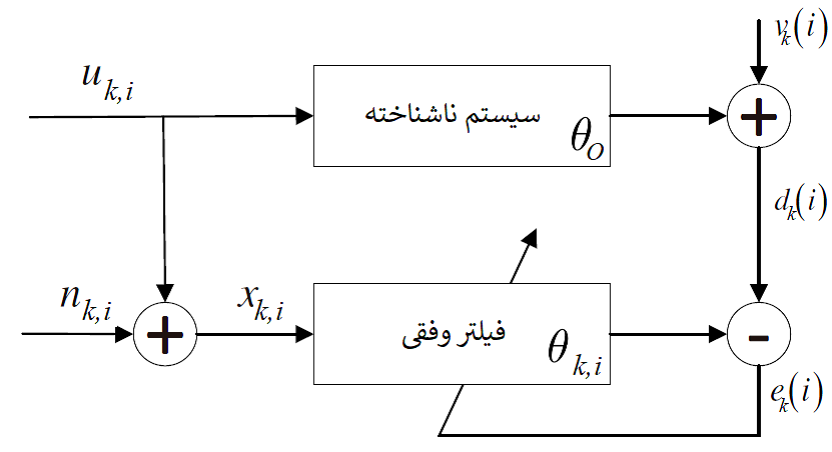
\includegraphics[scale=0.6]{Pic24.png}
		\caption{شبكه تطبيقي با نويز ورودي  \cite{Abdolee2016}}
		\label{p24}
	\end{center}
\end{figure}
در \cite{Naeimi2024_RClass} به منظور مقاوم‌سازی طبقه‌بندی آنلاین  با استفاده از روش یادگیری توزیع‌شده انتشاری از یک تابع خطا کسینوس لگاریتمی مشتق‌شده استفاده شده است  که برای نویزهای ضربه‌ای مناسب است.

حذف یا کاهش نویز و تداخل سیگنال صوتی یک فناوری پیشرفته است که امروزه  به منظور کاهش یا حذف صداهای ناخواسته و مزاحم در محیط‌های مختلف به کار میرود و یک چالش مهم در پردازش سیگنال می‌باشد. محققان روش‌های مختلفی از جمله روش‌های مبتنی بر فیلترهای تطبیقی ​​را برای رفع این مشکل معرفی کرده‌اند. در مقاله \cite{Bahraini2024_NoiseCncl} یک \lr{RLS} مقاوم مبتنی بر فیلتر تطبیقی با لگاریتم طبیعی و یک تابع خطا کسینوس هذلولی ارئه شده است که روشی را برای حذف نویز صوتی در برابر انواع خاصی از نویزها فراهم می‌کند. 

كارهاي انجام شده در زمينه مقاوم‌سازي رويكرد‌هاي توزيع‌شده مبتني بر انتشار در برابر نويز را با توجه به تابع هدف مي‌توان به دو دسته الگوريتم‌هاي مبتني بر حداقل‌سازي ميانگين مربعات خطا (\lr{MSE}) و الگوريتم‌هاي مبتني بر مفاهيم تئوري اطلاعات (\lr{ITL}) تقسيم كرد. اگر نويز موجود از مدل گوسي باشد، الگوريتم‌هاي مبتني بر حداقل‌سازي ميانگين مربعات خطا كه به واريانس نويز وابسته هستند، كارآيي مناسبي دارند. اما در برابر نويز غيرگوسي عملكرد مناسبي ندارند و در بعضی مواقع واگرا نيز مي‌شوند. به همين دليل، كارهايي ارائه شده است كه با جايگزين كردن \lr{MSE} با توابع هزينه مقاوم‌تر سعي بر مقابله با نويز‌هاي غيرگوسي دارند. در مقاله \cite{Li2013} الگوريتم حداقل آنتروپي خطا كه يكي از الگوريتم‌هاي مبتني بر تئوري اطلاعات است، بدين منظور استفاده شده است و در آن آنتروپي آخرين \lr{N} نمونه‌اي كه بيشترين ميزان خطا را دارند، به عنوان تابع هدف براي حداقل نمودن خطا استفاده مي‌شود. الگوريتم انتشار معيار حداكثرسازي کورآنتروپی (\lr{DMCC}) \cite{MA2016} از كرنل گوسي به دليل توانايي آن در رد كردن نمونه‌هاي آغشته به نويز غيرگوسي استفاده شده است. تابع هدف اين الگوريتم به صورت زير تعريف مي‌شود:
\begin{equation}\label{e143}
	\begin{cases}
		J_k^{local}(w)=\sum_{l\in N_k}c_{lk} G_{\sigma}(e^2_{l,k})\\
		G_{\sigma}(e^2_{l,k})=\frac{1}{\sigma \sqrt{2\pi}}\exp(-\frac{1}{2\sigma^2}(d_{l,i}-u_{l,i}w_l)^2)
	\end{cases}
\end{equation}

كه $G_{\sigma}(e^2_{l,k})$ تابع استاندارد گوسي با عرض كرنل $\sigma$ است.

الگوريتم‌هاي مبتني بر حداقل‌سازي ميانگين مربعات خطا با تغيير دادن تابع هدف سعي در مقاوم‌سازي در برابر نويز غيرگوسي دارند. الگوريتم انتشار علامت خطا \lr{DSignLMS} \cite{Ni2016} از علامت خطا در تابع هدف استفاده مي‌شود:
\begin{equation}\label{e144}
	\begin{cases}
		J_k^{local}(w)=\sum_{l\in N_k}c_{lk} \lvert\lvert e_{l,k}\rvert\rvert_1\\
		s.t. \lvert\lvert \phi_{k,i}-\theta_{k,i-1}\rvert\rvert^2_2\le\mu_k^2
	\end{cases}
\end{equation}

كه $\phi_{k,i}$ تخمين مياني در گره‌ $k$ام است و بردار گراديان اين الگوريتم به صورت $\nabla J_k^{local}(w)=\sum_{l\in N_k}c_{lk}u_{l,k}sgn(e_{l,k})$ محاسبه مي‌شود. 

در الگوريتم انتشار  \lr{DLMF} \cite{Park2014} ميانگين توان چهارم خطا در تابع هدف براي مقابله با نويز غيرگوسي به كارگرفته شده است. همچنين در الگوريتم انتشار \lr{RDLMS} \cite{Ashk} از تابع زيان شبه‌هابر\footnote{\lr{Pseudo-huber}} بدين منظور استفاده شده است. در \cite{Bert2011} روش‌هايي براي مقابله با داده‌هاي نويزي در الگوريتم \lr{RLS} مطرح شده است و همچنین در \cite{Naeimi2024_GMBZ} با معرفی تابع زیان جدیدی به نام \lr{GMBZ} به منظور مقاوم‌سازی در برابر نویزهای غیرگاوسی و کاهش تعدیل نادرست در حالت پایدار، الگوریتم مقاوم \lr{RLS} مبتنی بر تابع زیان \lr{GMBZ} ارائه داده‌اند. 

الگوريتم‌ها و رويكرد‌هايي كه تاكنون براي شبكه‌هاي تطبيقي توزيع‌شده مطرح‌شده‌‌اند، با فرض داشتن محیط همگام عمل مي‌كردند. با در نظر گرفتن اتفاقات تصادفي همچون زمان ورود داده‌ها، خرابي گره‌ها و لينك‌ها، تغييرات توپولوژي شبكه و غیره، در مقاله \cite{Zhao2014} پياده‌سازي الگوريتم انتشار با رويكرد \lr{ATC} به صورت زير در محيط غیرهمگام ارائه شده است.
\begin{equation}\label{e145}
	\begin{cases}
		\psi_k(i)=w_k(i-1)-\mu_k(i) \nabla_{w^T}J_k({w_k(i-1)})\qquad(Adapt)\\
		w_k(i)=\sum_{l\in N_{k,i}}a_{lk}(i)\psi_l(i)\qquad(Combine)
	\end{cases}
\end{equation}
كه در رويكرد غیرهمگام، پارامترهای $\mu_k(i)$ و $a_{lk} (i)$ با زمان تغییر می‌کنند و $N_{k,i}$ مجموعه همسایگی گره $k$ در زمان $i$ را بیان می‌کند. 

\subsection{نقاط ضعف روش‌های موجود}
به طور کلی، تمامی راه‌کارهایی که از روش‌های موجود استفاده می‌کنند شامل نقاط ضعف یکسانی می‌باشند. شکل \ref{Disadvantage} نقاط ضعف تمامی راه‌کار‌ها را با توجه به روش مورد استفاده نشان می‌دهد. 
 
\begin{figure}
	\begin{center}
		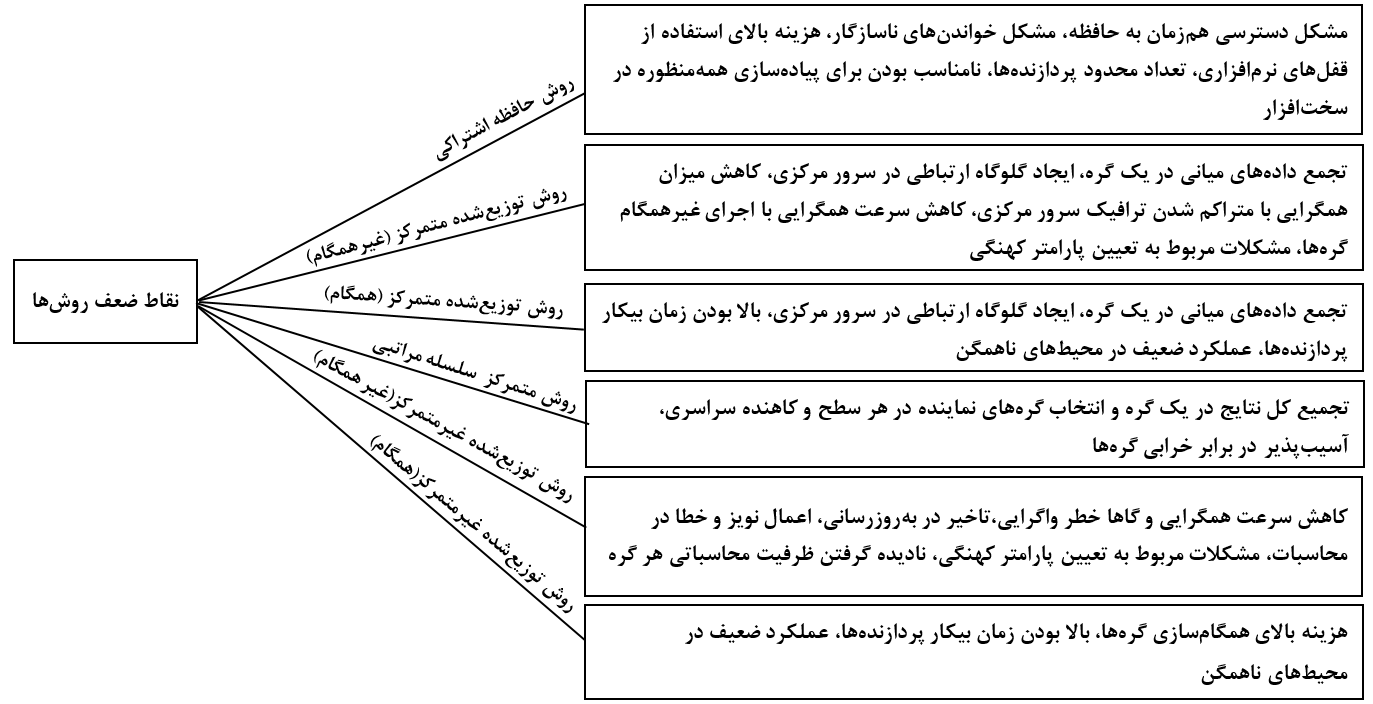
\includegraphics[scale=0.7]{DisAd_.PNG}
		\caption{بیان نقاط ضعف راه‌کارهای موجود}
		\label{Disadvantage}
	\end{center}
\end{figure}

روش‌های حافظه اشتراکی و حافظه اشتراکی توزیع‌شده همانند ماشین‌های \lr{NUMA} از مشکلات بسیاری رنج می‌برند، از جمله 1) محدود بودن تعداد پردازنده‌ها، 2) عدم مناسب بودن برای پیاده‌سازی‌های همه منظوره در سخت‌افزار و همچنین 3) دسترسی هم‌زمان پردازنده‌ها به حافظه اشتراکی و 4) عملیات خواندن ناسازگار. در برخی از تحقیقات به منظور همگام‌سازی پردازنده‌ها و جلوگیری از رخ دادن مشکلات ذکر شده، از قفل‌های نرم‌افزاری استفاده شده است که این قفل‌ها هزینه بالایی را متحمل می‌کنند. 

روش‌های توزیع‌شده یا شبکه‌های کامپیوتری متمرکز به دلیل استفاده از سرورهای مرکزی درگیر مشکلاتی از جمله تجمع داده‌های میانی در یک یا چند گره مرکزی، ایجاد گلوگاه ارتباطی، شلوغ شدن بار ترافیکی در سرورهای مرکزی و کاهش میزان همگرایی با متراکم شدن ترافیک در سرور مرکزی، می‌باشند. در صورتی که روش‌های توزیع‌شده متمرکز به صورت غیرهمگام اجرا شوند، شامل نقاط ضعف کاهش سرعت همگرایی با اجرای غیرهمگام  و تعیین پارامتر کهنگی خواهند بود. در مقابل روش‌های توزیع‌شده متمرکز همگام از نقاط ضعف بالا بودن زمان بیکاری گره‌ها و عملکرد ضعیف در محیط‌های اجرایی ناهمگن رنج می‌برند. 

روش‌های توزیع‌شده متمرکز سلسله مراتبی که از یک ساختار کلاینت-سرور چند سطحی استفاده می‌کنند، شامل نقاط ضعفی همانند انتخاب گره‌های نماینده در هر سطح و انتخاب کاهنده‌ سراسری و آسیب ‌پذیری در برابر خرابی گره‌ها و یال‌ها می‌باشند. 

روش‌های توزیع‌شده غیرمتمرکز دیگر درگیر مشکلاتی از جمله گلوگاه شدن سرور مرکزی و کاهش میزان همگرایی با متراکم شده ترافیک در سرور مرکزی و آسیب پذیری در برابر خرابی گره‌ها و یال‌ها، نیستند. اما اگر این روش‌ها به صورت غیرهمگام اجرا شوند، متحمل مشکلاتی از جمله کاهش سرعت همگرایی به دلیل استفاده از داده‌های غیرهمگام تبادل‌شده توسط پردازنده‌ها، تعیین پارامتر کهنگی  به منظور جلوگیری از کاهش سرعت همگرایی پردازنده‌ها، اعمال نویز و خطا در محاسبات پردازنده‌ها به دلیل استفاده از داده‌های کهنه و غیرهمگام و همچنین در نظر نگرفتن ظرفیت محاسباتی پردازنده‌ها در عملیات یادگیری، می‌باشند. روش‌های توزیع‌شده غیرمتمرکز همگام نیز با مشکلات خاص خود درگیر می‌باشند. هزینه بالای همگام‌سازی پردازنده‌ها با یکدیگر، بالا بودن زمان انتظار و بیکاری آنها و همچنین عملکرد ضعیف در محیط‌های اجرایی ناهمگن برخی از این مشکلات می‌باشند.  


\section{خلاصه}
در این فصل مطالعاتی در مورد نحوه اجرای روش‌های یادگیری توزیع‌شده بر روی سیستم‌های حافظه اشتراکی و سیستم‌های حافظه توزیع‌شده انجام شده است. این مطالعات با توجه به راه‌حل‌هایی که وجود داشت به دو بخش تقسیم شده‌اند. بخش اول مربوط به راه‌حل‌هایی است که یادگیری توزیع‌شده را بدون هیچ مدل محاسباتی انجام داده‌اند. در بخش دوم راه‌حل‌های یادگیری توزیع‌شده مبتنی بر مدل محاسباتی و پژوهش‌های انجام شده در این زمینه مورد مطالعه و بررسی گرفته است. سپس نقاط ضعف هر یک از روش‌ها به صورت خلاصه بیان شده است. در انتها، الگوریتم‌های یادگیری توزیع‌شده انتشاری موجود به عنوان الگوریتم یادگیری مورد استفاده در شبکه‌های تطبیقی توزیع‌شده مورد بررسی و مطالعه قرار گرفتند. 





\chapter{روش پیشنهادی}

\newpage
‎\renewcommand{\baselinestretch}{2}\normalsize‎
\label{ProposedApproach}

در این فصل روش پیشنهادی برای یادگیری توزیع‌شده در شبکه‌های تطبیقی ناهمگن با هدف کاهش ارتباطات در زمان اجرا و کاهش زمان انتظار گره‌ها و مقابله با مساله کندکننده‌ها ارائه خواهد شد. در ابتدا مقدمات و کلیات روش شرح داده شده و در ادامه جزئیات هر قسمت و تحلیل همگرایی و پایداری روش پیشنهادی بحث خواهد گردید.
\section{روش پیشنهادی}
همان گونه که در بخش تعریف مسئله مطرح شد، هدف از این پژوهش بدین صورت است که با استفاده از مفاهیم موازی‌سازی یک رویکرد یادگیری توزیع‌شده برای تخمین پارامترهای مسائل بهینه‌سازی در شبکه‌های تطبیقی توزیع‌شده ارائه داد. این رویکرد یادگیری توزیع‌شده مبتنی بر یک مدل محاسباتی موازی توسعه‌یافته به نام \lr{BSP} فدرالی (\lr{FBSP}) است که با توجه به خصوصیات شبکه‌های تطبیقی توزیع‌شده توسعه‌ یافته است. 

رویکردهای یادگیری توزیع‌شده به سه دسته همگام، غیرهمگام متمرکز و غیرهمگام غیرمتمركز تقسيم مي‌شوند. الگوریتم‌های همگام در یک محیط ناهمگن عملکرد ضعیفی دارند و الگوریتم‌های غیرهمگام متمرکز از مشکل گلوگاه ارتباطی در سرورهای پارامتر با افزایش تعداد گره‌ها و كاهش ميزان همگرايي با متراكم شدن ترافيك سرور پارامتر  رنج می‌برند. در این رساله به دنبال ارائه یک رویکرد موازی برای شبکه‌های تطبیقی توزیع‌شده هستیم که در عین کارآمد بودن ارتباطات و حفظ بهترین میزان همگرایی، در یک محیط ناهمگن نیز مقاوم باشد. در يك محيط ناهمگن سرعت محاسبه و ارتباطات گره‌های شبکه متفاوت خواهد بود. این امر به ویژگی‌های معماری، اشتراک منابع (به عنوان مثال، محاسبات ابری) و بد عمل كردن سخت افزار وابسته است. از آنجایی‌که هدف این نوع شبکه‌ها تخمین بردار پارامترهای بهینه از طریق تعامل و همکاری بین گره‌های مختلف بدون حضور یک سرور مرکزی است و همچنین به دلیل عدم نیاز انتظار هر گره برای سایر گره‌های شبکه و همچنین عدم نیاز به قفل‌گذاری‌های هزینه‌بر، الگوریتم‌های موازی‌سازی غیرهمگام غیرمتمرکز انتخاب مناسبی برای این شبکه‌ها می‌باشند. 

رویکرد پیشنهادی یک رویکرد داده-موازی است که هر گره بر روی داده‌های محلی خودش فرآیند یادگیری را انجام خواهد داد و در دو مرحله اصلی برون‌خط و برخط اجرا می‌شود. مرحله برون‌خط که مرحله پیش‌پردازش نیز نامیده می‌شود، شامل دو بخش رصدکردن شبکه و منطقه‌بندی شبکه است. در بخش رصد کردن شبکه، توان پردازشی هر گره محاسبه می‌شود. در بخش منطقه‌بندی شبکه، خوشه‌بندی گره‌ها براساس فاصله گره‌ها از همدیگر، توان پردازشی و میزان اعتماد بین گره‌ها انجام می‌شود. در مرحله برخط، فرآیند یادگیری موازی تحت مدل محاسباتی \lr{BSP} فدرالی بر روی شبکه تطبیقی توزیع‌شده که در مرحله پیش‌پردازش منطقه‌بندی شده است، اجرا خواهد شد. 

این مدل همانند مدل \lr{BSP} از سه بخش اصلی محاسبه، ارتباط و همگام‌سازی مانعی تشکیل شده است. با این تفاوت که مرحله ارتباط و همگام‌سازی مانعی در مدل \lr{BSP} فدرالی بر اساس یک روش منطقه‌بندی‌ انجام می‌شود. برای همگام‌سازی گره‌های شبکه در این رویکرد یک تکنیک همگام‌ فدرالی معرفی شده است که گره‌ها به صورت منطقه‌بندی شده و با قبول یک میزان کهنگی در سطح کل گره‌های شبکه همگام می‌شوند. به عبارت دیگر، همگام‌سازی در دو سطح منطقه‌ای و سراسری اجرا خواهد شد. در سطح منطقه‌ای، گره‌های همسایه‌ای با هم همگام می‌شوند که از لحاظ توان محاسباتی بهم شبیه‌ و از لحاظ فاصله ساختاری و میزان اعتماد بهم نزدیک باشند. در سطح سراسری، هر گره با گره‌های همسایه‌اش در کل شبکه همگام می‌شود. این روش منطقه‌بندی سبب می‌شود هزینه ارتباطات بین گره‌ها در زمان اجرا کاهش یابد و از رخ دادن مشکل کندکننده‌ها جلوگیری شود. در ادامه، بخش‌های مختلف راه‌کار پیشنهادی با جزئیات کامل شرح داده شده است.

\section{متغیرهای استفاده شده}
مجموعه متغیرهای استفاده شده در این رساله در جدول \ref{notation} آورده شده است.
\begin{table}[h]	
	\centering
	\caption{\small{متغیرهای مورد استفاده در مدل ریاضی سیستم پیشنهادی}}
	\label{notation}
	\footnotesize\rm
	\begin{tabular}{cc}
		\hline
		متغیر&توصیف\\
		\hline
		$N$&تعداد گره‌ها در شبکه\\
		$M$&مرتبه فیلتر یا اندازه بردار پارامترها\\
		$w_{k,t}$&بردار پارامترها گره \lr{k} در تکرار \lr{t}\\
		$\mu_{t}$&اندازه گام در تکرار \lr{t}\\
		$M^{(r)}$&مجموعه گره‌ها در منطقه \lr{r}\\
		$N^{(r)}$&تعداد گره‌ها در منطقه \lr{r}\\
		$U^{(i)}$&مجموعه داده آموزشی محلی گره \lr{i}\\
		$N_i^{(r)}$&مجموعه همسایگی گره \lr{i} در منطقه \lr{r}\\
		$N_i$&مجموعه همسایگی گره \lr{i} در کل شبکه\\
		
		\hline
	\end{tabular}
\end{table}

\section{الگوریتم یادگیری پیشنهادی}
در راستای ارائه رویکرد پیشنهادی، در این بخش یک الگوریتم يادگيري تطبیقی انتشاري به نام \lr{DSGD} (\lr{DiffusionSGD}) بر اساس استراتژی "تطبیق سپس ترکیب" (\lr{ATC}) و الگوریتم گرادیان کاهشی تصادفی مرتبه دوم معرفی می‌گردد.

\subsection{الگوریتم یادگیری تطبیقی انتشاری}
در شکل \ref{p12} یک شبکه تطبیقی با 10 گره نشان داده شده است که بر روی هر گره آن یک فیلتر تطبیقی اجرا خواهد شد. در روش یادگیری پیشنهادی، هر فیلتر تطبیقی مبتنی بر الگوریتم گرادیان کاهشی تصادفی است. در شکل \ref{p13} یک شمای کلی از چنین فیلتری در یک شبکه تطبیقی توزیع‌شده برای کاربرد شناسایی سیستم نشان داده شده است.
\begin{figure}[h]
	\begin{center}
		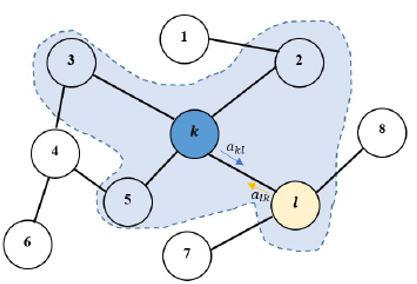
\includegraphics[scale=0.8]{Pic12.JPG}
		\caption{نمایش گرافیکی از یک شبکه تطبیقی با $N=10$ گره}
		\label{p12}
	\end{center}
\end{figure} 


\begin{figure}[h]
	\begin{center}
		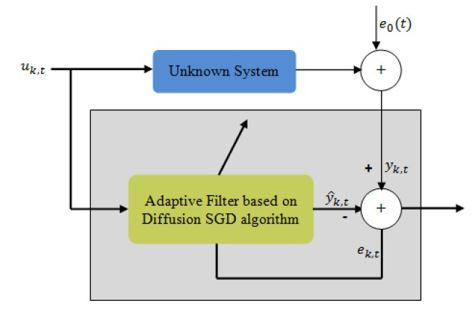
\includegraphics[scale=0.9]{Pic13.JPG}
		\caption{شمای کلی از فیلتر تطبیقی پیشنهادی در یک شبکه تطبیقی توزیع‌شده برای کاربرد شناسایی سیستم}
		\label{p13}
	\end{center}
\end{figure} 

روابط به‌روزرسانی وزن‌ها برای هر عامل $k$ در شبکه تطبیقی توزیع‌شده مبتنی بر الگوریتم گرادیان کاهشی تصادفی مرتبه دوم پس از حل مساله بهینه‌سازی $\min_w\sum_{k=1}^{N}E[\phi(w_ku_k,y_k)]+\frac{\lambda}{2}||w_k||^2_2$ به صورت زیر تعریف می‌شوند:
\begin{equation}\label{e20}
	\begin{cases}
		\psi_{k,t}=w_{k,t-1}-\mu_{t} S_t^{-1} \frac{\partial}{\partial w}[\phi(w_{k,t-1}u_{k,t},y_{k,t})+\frac{\lambda}{2}||w_{k,t-1}||^2_2]\\
		w_{k,t}=\sum_{l\in N_k} a_{lk} \psi_{l,t}
	\end{cases}
\end{equation}
که $\phi(w_{k,t}u_{k,t},y_{k,t})$ تابع زیان گره $k$ در تکرار $t$ است و  با ادغام روابط \textbf{تطبیق} و \textbf{ترکیب} در \ref{e20}، رابطه به‌روزرسانی استفاده شده برای بردار پارامترها $w_{k,t}$ گره $k$ در تکرار $t$ به صورت زیر بدست می‌آید:
\begin{equation}\label{ww}
	w_{k,t}=\sum_{l\in N_k} a_{lk}w_{l,t-1}-\mu_{t} S_t^{-1} \sum_{l\in N_k} a_{lk}(\phi^{'}(w_{l,t-1}^T u_{l,t},y_{l,t})u_{l,t}+\lambda w_{l,t-1})
\end{equation}
الگوریتم یادگیری توزیع‌شده انتشاری پیشنهادی در شبه‌کد \ref{Alg_DSGD} آورده شده است.

\begin{latin}
	

\begin{algorithm}
	\caption{ The ATC Diffusion SGD algorithm}\label{Alg_DSGD}
	\begin{algorithmic}
		\State Initialize $ w_{l,0}=0$ for $l\in\{1,2,...,N\}$
		\State Given non-negative real coefficients \{$a_{l,k}$\} satisfying the conditions in Eq.\ref{e8}
		\State Given suitable step-size parameter $\eta_t>0$
		\For {$t\in\{1,2,...,T\}$}
			\For   {each node $k\in\{1,2,...,N\}$}
				\State Draw example $<\textbf{u}_{k,t},y_{k,t}>\in D$ randomly
				\State Execute the adaptive step of diffusion SGD and Compute $\psi_{k,t}$
				\State Execute the combine step of diffusion SGD and Compute $w_{k,t}$
			\EndFor
		\EndFor
	\end{algorithmic}
\end{algorithm}
\end{latin}

الگوریتم یادگیری توزیع‌شده پیشنهادی در این بخش در حالت کلی و بدون در نظر گرفتن تابع زیان مشخصی معرفی شد. تابع زیان یک تابع ریاضی است که تفاوت بین مقادیر پیش‌بینی شده توسط الگوریتم یادگیری و مقادیر واقعی را کمینه‌سازی می‌کند. در واقع عملکرد الگوریتم یادگیری را اندازه‌گیری می‌کند و فرآیند بهینه‌سازی را با ارائه بازخورد در مورد میران نزدیکی جواب با داده‌ها هدایت می‌کند. توابع خطا مختلفی تا کنون ارائه شده است که هر یک ویژگی‌ها و قابلیت‌های متفاوتی دارد. 

وجود داده‌های پرت و انواع نویز در محیط‌های یادگیری اجتناب ناپذیری است که باعث می‌شوند عملکرد الگوریتم‌های یادگیری توزیع‌شده به شدت کاهش یابد. برخی از توابع خطا در برابر نویزها و داده‌‌های پرت مقاوم نیستند، در نتیجه عملکرد الگوریتم یادگیری را به شدت تحت تاثیر قرار می‌دهند. در بخش بعدی، تعدادی از توابع خطا مناسب حل مسائل رگرسیون معرفی می‌گردند و سپس الگوریتم یادگیری توزیع‌شده مقاوم ارائه می‌شود. 	
\subsection{الگوریتم یادگیری تطبیقی انتشاری مقاوم}
استفاده از توابع زیان مقاوم در برابر نویزهای مختلف محیطی سبب افزایش مقاومت روش یادگیری توزیع‌شده پیشنهادی می‌شود. تابع زیان مربع خطا\footnote{\lr{Square Loss function}}  تنها در برابر نویزهای گاوسی مقاوم است اما در محیط‌های آغشته به نویزهای غیرگاوسی عملکرد ضعیفی دارد و در اکثر مواقع واگرا می شود. توابع زیانی مانند شبه‌هابر\footnote{\lr{Pseudo-Huber}} ، کورانتروپی\footnote{\lr{Correntropy}}  و ... نسبت به نویزهای غیرگاوسی مقاوم می‌باشند. 

تابع زیان ‌هابر برای مقادیر بزرگ خطا $e$ خطی و برای مقادیر کوچک آن از درجه دوم می‌باشد. تابع زیان شبه‌هابر یک تقریب مشتق‌پذیر نرم از تابع زیان هابر می‌باشد که ترکیبی از توابع هزینه مربعی و قدرمطلق است. مزیت اصلی این تابع نسبت به تابع زیان هابر این است که دوبار مشتق‌پذیر و نرم است و نسبت به نویز گاوسی و همچنین نویزهای غیرگاوسی مقاوم می‌باشد.
\begin{equation}
	L_{\delta}(e)=
	\begin{cases}
		\frac{1}{2}e^2\qquad if \quad |e|<\delta\\
		\delta(|e|-\frac{1}{2}\delta)\qquad otherwise
	\end{cases}
	Huber Loss
\end{equation}

\begin{equation}
	L_{\delta}(e)=\delta^2(\sqrt{1+(e/\delta)^2}-1)\qquad Pseudo-Huber Loss
\end{equation}
که $e$ خطا فیلتر و $\delta$ یک پارامتر اضافی برای کنترل شیب در مقادیر بزرگ خطا است. 

تابع زیان کورآنتروپی \cite{CorrEntrop} که در الگوریتم‌های یادگیری تئوری اطلاعات استفاده می‌شود، به صورت زیر تعریف می‌گردد: 
\begin{equation}
	j_k (w)=1-\exp⁡(- \frac{e^2}{2\eta^2})      \qquad Correntropy Loss
\end{equation}

که $\eta$ پارامتر خطا کورآنتروپی می‌باشد که پهنای باند کرنل را تنظیم می‌کند. تایع زیان کورآنتروپی نسبت به داده‌های پرت و نویزهای ضربه‌ای مقاوم است و در محیط‌هایی که دارای نویز غیرگاوسی می‌باشد، بسیار مناسب خواهد بود. این تابع زیان با پهنای باند کمتر، تابع‌ نرم‌تر و نسبت به نویز مقاوم‌تر می‌باشد. 

در مقاله \cite{Barron17} یک تابع زیان کلی مقاوم و تطبیقی معرفی شده است که در واقع تعمیمی از تعدادی تابع زیان از جمله مربع خطا، شبه هابر، \lr{Charbonnier} تعمیم یافته،  \lr{Cauchy/Lorentzian} \cite{CauchyLoss}، \lr{Welsch/Leclerc} \cite{WelschLoss}و \lr{Geman-McClure} \cite{GemanLoss} است. 

\begin{equation}\label{GenralLosses}
	L(e,\alpha,c)=\frac{|\alpha-2|}{\alpha}\left((\frac{(\frac{e}{c})^2}{|\alpha-2|}+1)^{\frac{\alpha}{2}}-1\right) 
\end{equation}
که $\alpha\in \mathbb{R}$ پارامتری برای کنترل مقاومت خطا است و $c>0$ هم یک پارامتر مقیاس برای کنترل اندازه کاسه درجه دوم خطاها در نردیکی $a=0$ است. به ازای $\alpha=2$ و $\alpha=1$ رفتار آن به ترتیب نزدیک به تابع زیان مربع خطا و شبه هابر است. زمانیکه $\alpha\rightarrow 0$، خطا کوشی یا \lr{Cauchy} و $\alpha=-2$ خطای \lr{Gman-McClure} را سبب می‌شود. همچنین زمانیکه $\alpha\rightarrow -\infty$، خطا \lr{Welsch} را خواهیم داشت.  در ادامه روابط این توابع خطا به صورت مجزا آورده شده است.
	\begin{flalign}
	&L(e,c)=1-\exp(-\frac{1}{2}(\frac{e}{c})^2) \qquad Welsch/Leclerc \quad Loss\\
	&L(e,c)=\log(\frac{1}{2}(\frac{e}{c})^2+1) \qquad \quad Cauchy/Lorentzian \quad Loss\\
	&L(e,c)=\frac{2(\frac{e}{c})^2}{(\frac{e}{c})^2+4} \qquad \quad \qquad Geman-McClure \quad Loss
\end{flalign} 
تابع زیان شبه‌هابر مشتق‌پذیر است و نرم‌تر از سایر توابع زیان بوده و نسبت به تابع زیان مربع خطا کمتر به نویز در داده‌های ورودی و داده‌های پرت حساس است. با در نظر گرفتن عواملی چون سادگی، مقاومت در برابر انواع خطاهای محیطی و نرم بودن، تابع زیان شبه‌هابر به عنوان تابع زیان الگوریتم یادگیری پیشنهادی انتخاب می‌شود. بر این اساس، تابع هزینه محلی $J_k(w)$ هر گره $k$ به صورت زیر خواهد بود:

\begin{equation}\label{Jk}
	J_k(w)=\delta^2(\sqrt{1+(\frac{e_k}{\delta})^2}-1)
\end{equation}
تابع هزینه $J_k(w)$  قویا محدب بوده و $\nabla^2J_k(w)$ یک ماتریس هسین مثبت معین است.  مشتق $J_k(w)$ با توجه به $w$ در تکرار $t$ به صورت زیر است:
\begin{equation}\label{deriv_Jk}
	\nabla J_k(w)=-\frac{e_k(t)u_{k,t}^T}{\sqrt{1+(\frac{e_k(t)}{\delta})^2}}
\end{equation}

با جایگذاری \ref{deriv_Jk} در \ref{ww} به عنوان مشتق تابع زیان $\phi$، رابطه به‌روزرسانی بردار پارامترها برای هر گره $k$ در روش یادگیری توزیع‌شده پیشنهادی مبتنی بر تابع زیان شبه‌هابر و براساس استراتژی "تطبیق سپس ترکیب"، به صورت زیر ارائه می‌شود:
\begin{equation}\label{complete_w}
	w_{k,t}=\sum_{l\in N_k}a_{lk}w_{l,t-1}-\mu S^{-1}_t \lambda(\sum_{l\in N_k}a_{lk}w_{l,t-1})+\mu S^{-1}_t (\sum_{l\in N_k}a_{lk}\frac{e_l(t)u_{l,t}^T}{\sqrt{1+(\frac{e_l(t)}{\delta})^2}})
\end{equation}

همانطور که قبلاً ذکر شد، $S^{-1}_t$ به عنوان پیش شرطی است که در صورت انتخاب یک مقدار مناسب برای آن می‌توان نرخ همگرایی الگوریتم را بهبود بخشد. در این رساله، ما $S^{-1}_t$ را با استفاده از رابطه بازگشتی زیر در هر تکرار تعیین می‌کنیم:
\begin{equation}\label{S_inv}
	\begin{cases} 
		S^{-1}_0=\xi I_M\\\\
		Gain_t=\frac{S^{-1}_{t-1} u_{k,t}} {\gamma+u_{k,t}^T S^{-1}_{t-1} u_{k,t}}\\\\
		S^{-1}_t=S^{-1}_t - Gain_t u^T_{k,t} S^{-1}_t
	\end{cases}
\end{equation}
که $\xi$ یک مقدار ثابت است و $I_M$ نشان‌دهنده یک ماتریس همانی به ابعاد $M \times M$ است. $S_t^{-1}$ برای هر نمونه ورودی یا هر دسته داده ورودی در هر تکرار به روز می‌شود. در صورت وارد شدن نویز به داده‌های خروجی، مدل داده با اعمال نویز به صورت

\begin{equation}\label{modelee}
	d_k (t)=w_o^T u_k (t)+\nu_k (t)
\end{equation}

 است. در این مدل داده، ترم $\nu_k (t)$ نشان‌دهنده یک فرآیند نویز افزاینده با میانگین صفر یا همان نویز سفید گوسی است که مستقل از داده‌های ورودی $u_k (t)$ است. الگوریتم یادگیری توزیع‌شده مقاوم پیشنهادی \lr{RDSGD} (\lr{Robust DiffusionSGD}) در شبه‌کد \ref{Alg_RDSGD} آورده شده است. 
\begin{latin}
	

	\begin{algorithm}
	\caption{The ATC form of RDSGD algorithm}\label{Alg_RDSGD}
	\begin{algorithmic}
		\State Parameters: $\lambda$, $0<\gamma<1$, $\mu>0$
		\State Initialization: $ w_{k,0}=0$ for $l\in\{1,2,...,N\}$
		\State Set the coefficients \{$a_{l,k}$\} based on the conditions in Eq.\ref{e8}
		\For {$t\in\{1,2,...,T\}$}
			\For   {each node $k\in\{1,2,...,N\}$}
				\State Draw sample $(\textbf{u}_{k,t},y_{k,t})$ randomly
				\State Estimation error: \\\qquad$e_k(t)=d_k(t)-w_{k,t-1}^T\textbf{u}_{k,t}$
				\State Adaptive step: \\\qquad$\psi_{k,t}=w_{k,t-1}-\mu_k S_t^{-1}\left(\lambda w_{k,t-1}-\frac{e_k(t)\textbf{u}_{k,t}^T}{\sqrt{1+(\frac{e_k(t)}{\delta})^2}}\right)$
				\State Combination step: \\\qquad$w_{k,t}=\sum_{l\in N_k}a_{lk}\psi_{l,t}$
			\EndFor
		\EndFor
	\end{algorithmic}
\end{algorithm}
\end{latin}

\subsection{کاربرد الگوریتم یادگیری پیشنهادی در مساله پیش‌بینی}
یکی از کاربردهای مهم این الگوریتم پیشنهادی، مساله پیش‌بینی است. در این رساله توانایی الگوریتم یادگیری را در پیش‌بینی داده‌های بورس ایران مورد ارزیابی قرار خواهیم داد. روابط پیشنهادی برای مدل کردن مساله پیش‌بینی به صورت زیر می‌باشند:
\begin{equation}
	\begin{cases}
		\hat{d}_k(t)=w_{k,t}^T\dot{d_k (t:-1:t-M)}\\
		e_k(t)=d_k(t+1)-\hat{d}_k(t)
	\end{cases}
\end{equation}

\begin{equation}
	\begin{cases}
		\psi_{k,t}=w_{k,t-1}-\mu S^{-1}(\lambda w_{k,t-1}+\frac{d_k(t:-1:t-M)^T e_k(t)}{\sqrt{1+(\frac{e_k(t)}{\delta})^2}})\\
		w_{k,t}=\sum_{l\in N_k}a_{lk}\psi_{l,t}
	\end{cases}
\end{equation}

\section{رویکرد یادگیری توزیع‌شده پیشنهادی}

در این بخش به معرفی رویکرد یادگیری توزیع‌شده پیشنهادی که متناسب با خصوصیات شبکه‌های تطبیقی توزیع‌شده است با جزئیات پرداخته می‌شود. همان‌طور که قبلا هم اشاره شده است، رویکرد پیشنهادی در دو مرحله اصلی برون‌خط و برخط اجرا می‌شود. شکل \ref{p14} نمودار جریان کلی رویکرد یادگیری پیشنهادی را نشان می‌دهد. هما‌ن‌طور که دیده می‌شود، مرحله برون‌خط که مرحله پیش‌پردازش نیز نامیده می‌شود، شامل دو بخش رصد کردن\footnote{\lr{Monitoring}} شبکه و منطقه‌بندی\footnote{\lr{Regioning}} شبکه است. در بخش رصد کردن شبکه به محاسبه توان پردازشی هر گره پرداخته می‌شود. بدین منظور یک دسته‌داده با اندازه ثابت به هر گره داده می‌شود و زمان انجام آن محاسبه می‌شود. سپس زمان‌های بدست آمده نرمال خواهند شد. در بخش منطقه‌بندی شبکه، خوشه‌بندی گره‌ها براساس فاصله گره‌ها از همدیگر، توان پردازشی محاسبه‌شده در بخش قبلی و میزان اعتماد بین گره‌ها انجام خواهد شد. در مرحله برخط، فرایند یادگیری موازی مبتنی بر مدل محاسباتی پیشنهادی \lr{BSP} فدرالی (\lr{FBSP}) بر روی شبکه تطبیقی توزیع‌شده که در مرحله پیش‌پردازش منطقه‌بندی شده است، اجرا خواهد شد.
\begin{figure}[h]
	\begin{center}
		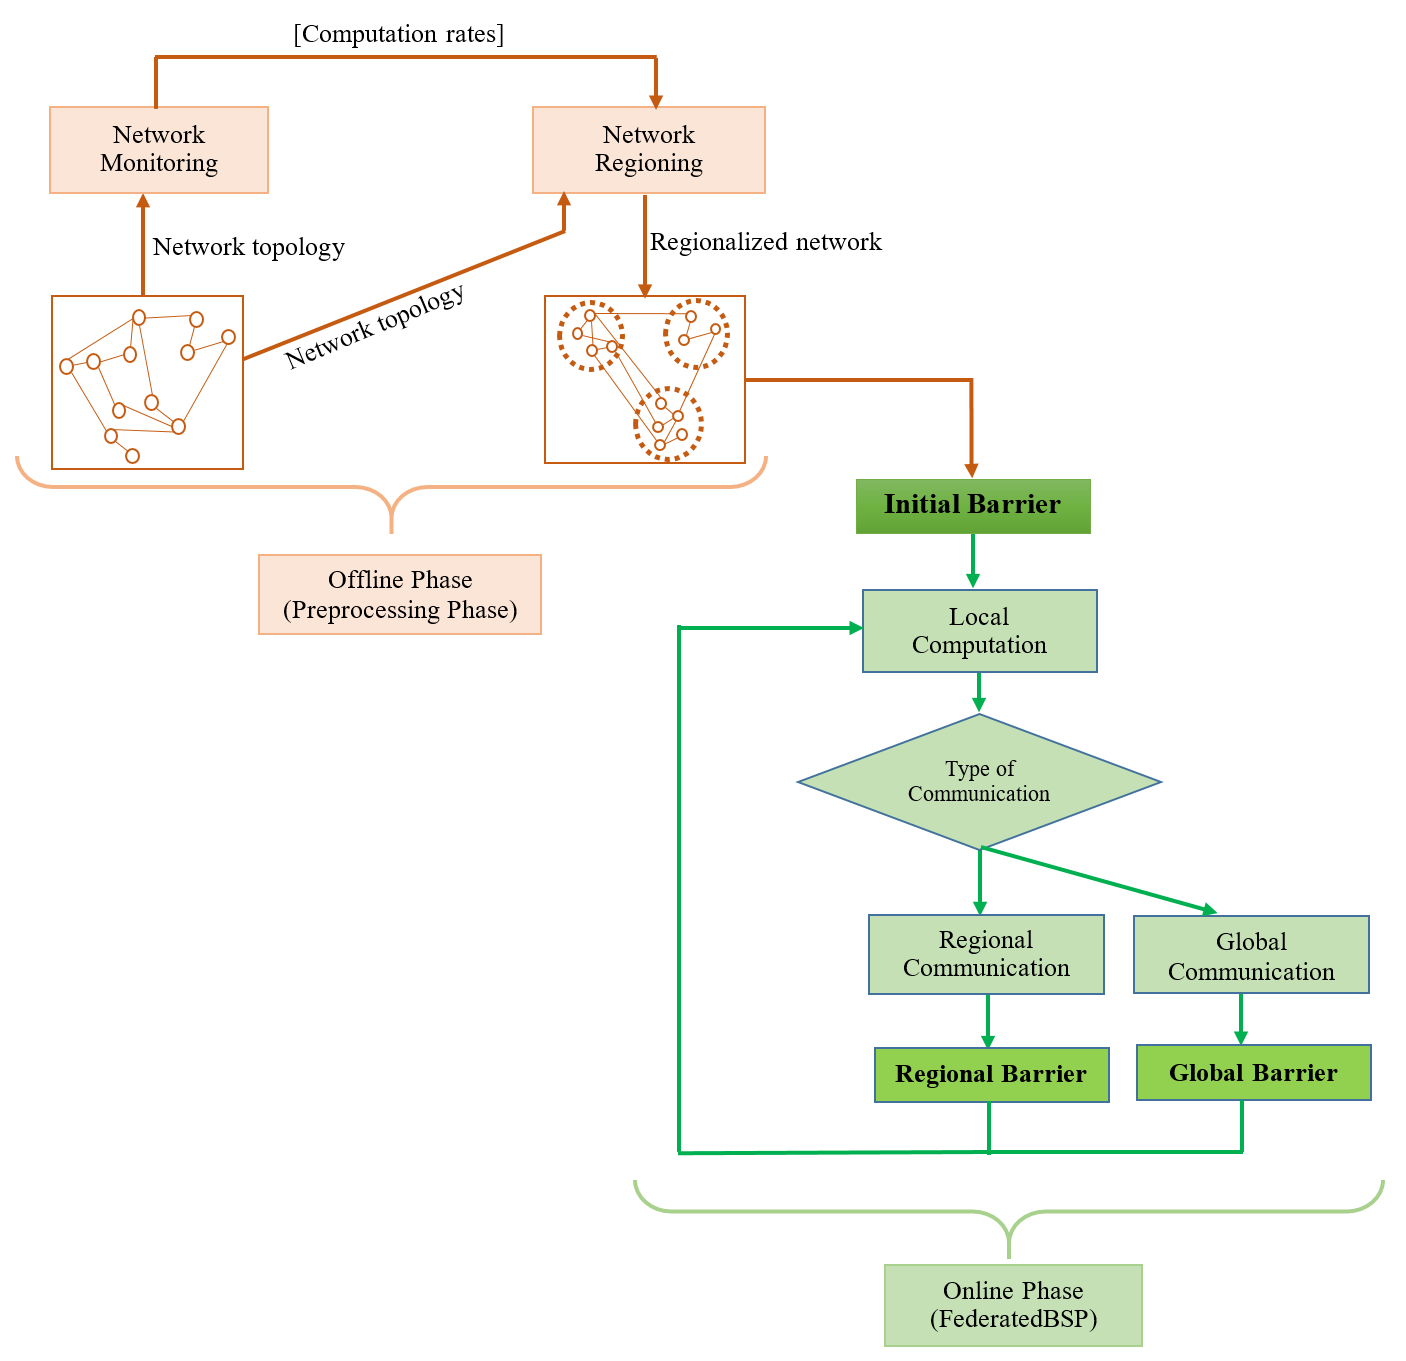
\includegraphics[scale=0.7]{Pic16.png}
		\caption{نمودار جریان رویکرد یادگیری پیشنهادی}
		\label{p14}
	\end{center}
\end{figure} 

\subsection{مدل محاسباتی پیشنهادی \lr{BSP} فدرالی یا \lr{FBSP}}
مدل محاسباتی \lr{BSP} فدرالی (\lr{FBSP}) همانند مدل محاسباتی \lr{BSP} از سه بخش مهم محاسبه، ارتباط و همگام‌سازی مانعی تشکیل شده است. با این تفاوت که بر اساس منطقه‌بندی انجام شده و همسایگی گره‌ها در شبکه، دو نوع ارتباط بین گره‌های شبکه شامل \textbf{ارتباط منطقه‌ای} و \textbf{ارتباط سراسری} در مدل \lr{BSP} فدرالی معرفی شده است. در ارتباط منطقه‌ای، هر گره با گره‌های همسایه‌اش در منطقه‌ای که قرار دارد ارتباط برقرار می‌کند و تبادل داده بین‌ آنها انجام می‌شود. در ارتباط سراسری، هر گره با گره‌های همسایه‌اش در کل شبکه ارتباط برقرار می‌کند و تبادل داده بین‌ آنها انجام می‌شود. به دنبال نوع ارتباط‌های متفاوت در مدل محاسباتی پیشنهادی، دو نوع همگام‌سازی مانعی شامل \textbf{همگام‌سازی مانعی منطقه‌ای} و \textbf{همگام‌سازی مانعی سراسری} معرفی شده است. همگام‌سازی مانعی منطقه‌ای بین گره‌های همسایه واقع در یک منطقه و همگام‌سازی مانعی سراسری بین گره‌های همسایه واقع در کل شبکه انجام خواهد شد. این کار سبب می‌شود میزان ارتباطات بین گره‌ها در زمان اجرا کاهش یابد و از رخ دادن مساله کندکننده‌ها جلوگیری شود. 

مساله کندکننده‌ها به یکی از دو دلیل 1) وجود گره‌های کند در بین گره‌های شبکه و 2) عدم توازن بار در بین گره‌‌ها، رخ خواهد داد. در صورتی که محیط توزیع‌شده یک محیط ناهمگن باشد، احتمال حضور گره‌های کند در شبکه بسیار بالا است که این موضوع افزایش زمان انتظار گره‌های سریع‌تر را نتیجه خواهد داد. در حالتی که داد‌ه‌های پردازشی در شبکه توزیع‌شده از نوع ویدیو یا هر داده دیگری با اندازه‌های متفاوت باشد، عدم توازن بار را در گره‌ها خواهیم داشت که سبب می‌شود برخی از گره‌ها با اندازه داده یا اندازه ویدیو کوچک‌تر محاسبات‌شان زودتر تمام شود که باید منتظر سایر گره‌ها برای اتمام کارشان بماند. در نتیجه زمان انتظار افزایش پیدا خواهد کرد. 

همان‌طور که قبلا هم اشاره شده است، همگام‌سازی یا مکانیزم کنترل مانع بین گره‌ها از اجزای مهم طراحی رویکردهای یادگیری توزیع‌شده است. مکانیزم‌های همگام‌سازی کنترل مانع به طور کلی به سه مکانیزم غیرهمگام (\lr{ASP})، همگام با کهنگی (\lr{SSP}) و همگام مانعی (\lr{BSP}) دسته‌بندی می‌شوند. شکل \ref{p17} مکانیزم همگام‌ مانعی پیشنهادی در مدل محاسباتی \lr{BSP} فدرالی را با روش‌های دیگر بر اساس معیارهای دقت همگرایی و توان عملیاتی آموزش (معکوس زمان اجرا تکرارها) مقایسه می‌کند.

\begin{figure}[h]
	\begin{center}
		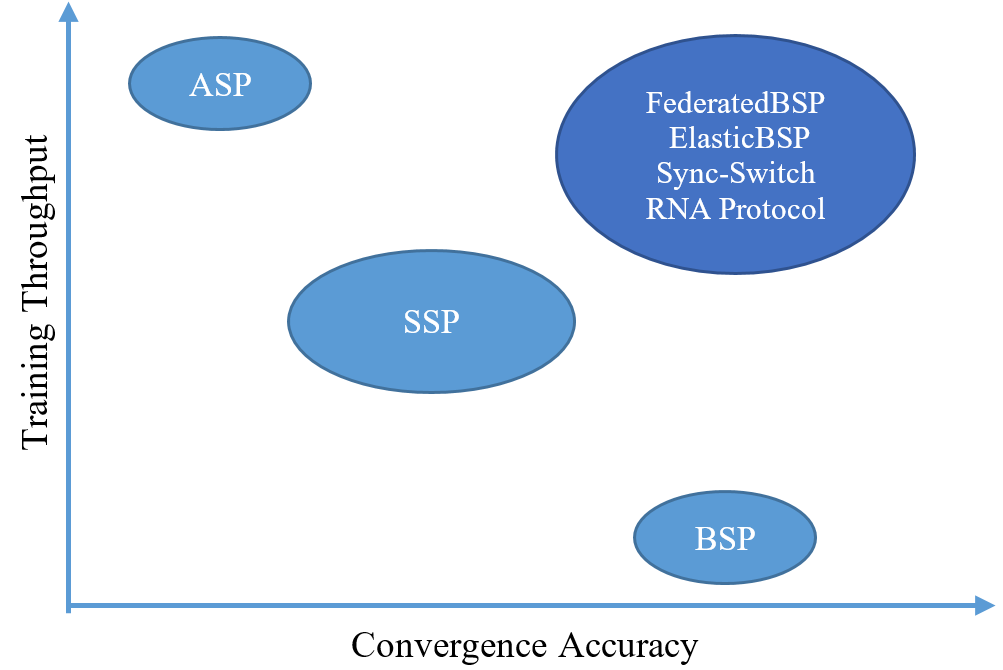
\includegraphics[scale=0.7]{Comp1.PNG}
		\caption{مقایسه مکانیزم همگام‌سازی مانعی پیشنهادی با سایر مکانیزم‌ها}
		\label{p17}
	\end{center}
\end{figure}

\subsection{مرحله رصد کردن شبکه}
مرحله رصد کردن به صورت یک مرحله برون‌خط و یک عملیات پیش‌پردازشی برای محاسبه توان کاری یا نرخ محاسباتی هر گره اجرا می‌شود. بدین منظور، توسط یک گره مرکزی به سایر گره‌ها در شبکه یک دسته داده با اندازه ثابت ارسال می‌شود. هر گره‌ پس از پردازش دسته داده، گرادیان محاسبه شده را به گره مرکزی ارسال می‌کند. بر این اساس گره مرکزی نرخ محاسباتی هر گره، میانگین زمان پردازش تمام گره‌های شبکه و سریع‌ترین و کندترین گره‌ها را مشخص می‌کند و این اطلاعات را به منظور منطقه‌بندی شبکه به مرحله بعدی ارسال می‌کند. 
در این مرحله بعد از محاسبه نرخ محاسباتی گره‌ها، اندازه دسته داده هر گره به صورت ضریبی از نرخ محاسباتی آن گره تعیین می‌گردد. به عبارتی، به گره‌های سریع‌تر اندازه دسته‌های بزرگتر و به گره‌های کندتر اندازه دسته‌های کوچک‌تری تخصیص داده می‌شود. این کار سبب می‌شود که زمان انتظار گره‌ها در زمان همگام‌سازی مانعی سراسری و همچنین میزان کهنگی پارامترهای مدل در بخش ارتباطات تا حدودی کاهش یابد و زمان محاسبه گره‌ها با نرخ‌های محاسباتی متفاوت نزدیک بهم شود. 


\subsection{مرحله منطقه‌بندی شبکه}
توپولوژی شبکه به صورت یک گراف ویژگی $G=(V,E,A)$ در نظر گرفته می‌شود، به‌طوریکه در آن $V$  مجموعه گره‌های شبکه، \lr{E} مجموعه یال‌های موجود بین گره‌ها و \lr{A} مجموعه خصوصیات هر گره را نشان می‌دهد. به هر گره $v_i\in V$ یک بردار ویژگی شامل نرخ پردازش محاسباتی گره $cp_i$ و ضرایب وزن همسایگی گره$[a_{1i},a_{2i},...,a_{ni}]$ تخصیص داده می‌شود. منطقه‌بندی گره‌های شبکه باید به صورتی انجام شود که هر کدام از منطقه‌ها علاوه‌بر نزدیکی ساختاری و وزن همسایگی، از لحاظ محتوایی نیز بهم شبیه باشند. بدین منظور در این مرحله، ابتدا گره‌ها بر اساس نرخ پردازش محاسباتی $cp_i$ و میانگین نرخ پردازش محاسباتی کل گره‌های شبکه $\bar{CP}$ ، برچسب‌گذاری می‌شوند. سپس از روش خوشه‌بندی ساختاری-محتوایی به نام \lr{ICS-cluster } \cite{Kesh2020} استفاده می‌شود. در این روش ابتدا ساختار و محتوای گراف اولیه ترکیب شده و یک گراف ساختاری-محتوایی ساخته می‌شود. وزن شباهت گره‌ها با استفاده از رابطه \ref{e21} محاسبه می‌شود. وزن شباهت گره‌های $i$ و $j$ که با $WS_{ij}$ نشان داده می‌شود به عنوان وزن یال بین آنها در گراف ساختاری-محتوایی ایجاد شده در نظر گرفته خواهد شد.

\begin{equation}\label{e21}
	WS_{ij}=a\times (\frac{1}{Dist(i,j)})+b\times Sim(i,j)+c*a_{ij}
\end{equation}

که $i\notin j$ است و $a$ ضریب شباهت ساختاری، $b$ ضریب شباهت محتوایی و $c$ ضریب وزن همسایگی میان گره $i$ و $j$ است. این ضرایب در فرآیند یادگیری مقدارشان تعیین می‌گردد. وزن همسایگی نشان‌دهنده میزان اطمینان و اهمیت اطلاعات دریافتی از گره همسایه است. مقدار $Sim(i,j)$ را با استفاده از معیارهای مختلف اندازه‌گیری شباهت همچون ضریب شباهت ژاکارد\footnote{\lr{Jaccard similarity}}  می‌توان محاسبه کرد. برای محاسبه شباهت ساختاری از عکس فاصله دو گره از یکدیگر استفاده می‌شود. در این رابطه هر چه فاصله دو گره بیشتر باشد، شباهت ساختاری کمتر خواهد بود. فاصله بین دو گره می‌تواند فاصله واقعی آنها از یکدیگر باشد یا برابر با تعداد یال‌های بین آنها در شبکه در نظر گرفته شود. به طور کل فاصله بین گره‌ها از طریق الگوریتم دایجسترا\footnote{\lr{Dijkstra algorithm}}  محاسبه می‌شود. 

بعد از محاسبه وزن‌های شباهت، میانگین این وزن‌ها $\bar{WS}$ در کل شبکه به عنوان یک حد آستانه برای ایجاد گراف ساختاری-محتوایی استفاده می‌شود. اگر $WS_{ij}$ از مقدار $\bar{WS}$ بیشتر باشد، بین دو گره $i$ و $j$ در گراف مورد نظر یالی رسم می‌شود. در غیر این صورت بین آن دو گره هیچ یالی در نظر گرفته نخواهد شد.

در گراف وزن‌دار حاصل، ابتدا هر گره به عنوان یک منطقه در نظر گرفته می‌شود. سپس به ترتیب گره‌هایی که یال‌های با وزن بالا دارند با یکدیگر ادغام شده و تشکیل یک منطقه را می‌دهند. تمام گره‌هایی که با چند یال به منطقه‌ای متصل هستند، به یک یال تبدیل شده و از وزن آن‌ها میانگین گرفته می‌شود و به عنوان وزن ارتباط آن گره با منطقه در نظر گرفته می‌شود. این فرآیند به صورت تکراری تا جایی ادامه می‌یابد که تعداد منطقه‌ها برابر با تعداد منطقه‌های موردنظر شوند. در فرآیند منطقه‌بندی با اعمال شرطی بر روی اندازه منطقه‌ها در زمان اجرا، متعادل‌سازی اندازه منطقه‌ها در نظر گرفته می‌شود. شکل \ref{p115} نمودار جریان الگوریتم خوشه‌بندی ساختاری-محتوایی مورد نظر را نشان می‌دهد که گراف اولیه و ماتریس شباهت ورودی‌های نمودار جریان و گراف خوشه‌بندی شده با تعداد خوشه‌های مورد نظر خروجی آن می‌باشند. به عنوان یک مثال برای واضح‌تر شدن روند کار این الگوریتم، در شکل \ref{p15} مراحل خوشه‌بندی ساختاری-محتوایی بر روی یک شبکه با ماتریس شباهت گره‌های آن نمایش داده شده است.
\begin{figure}[h]
	\begin{center}
		
		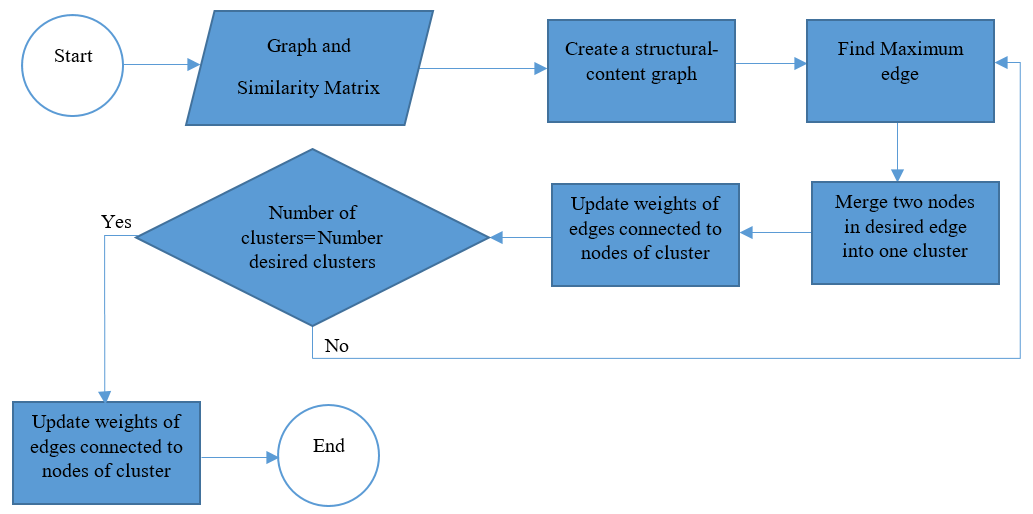
\includegraphics[scale=0.8]{icsCluster.PNG}
		\caption{نمودار جریان الگوریتم خوشه‌بندی ساختاری-محتوایی}
		\label{p115}
	\end{center}
\end{figure}

\begin{figure}[h]
	\begin{center}
		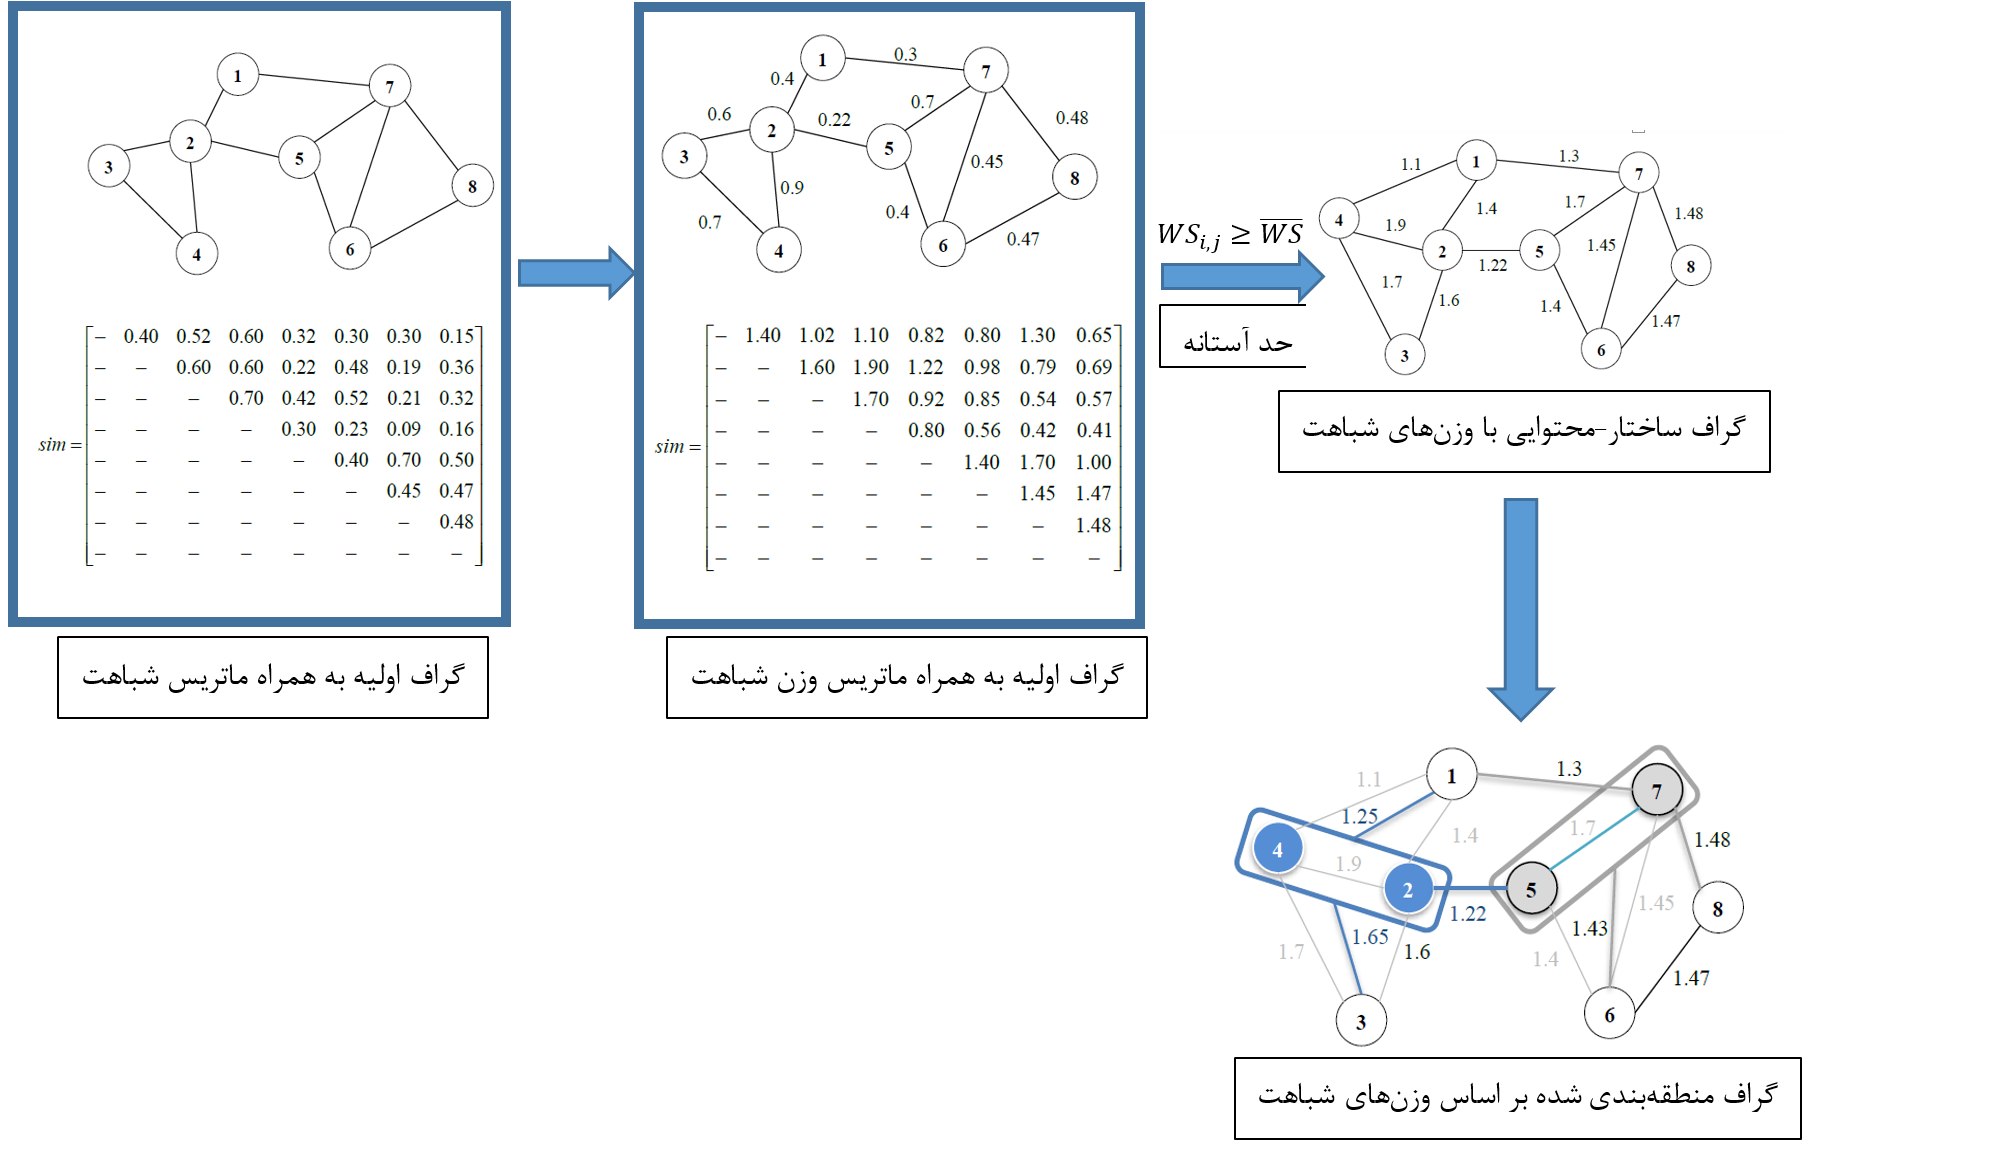
\includegraphics[scale=0.45]{Graph1.png}
		\caption{مراحل اجرای الگوریتم خوشه‌بندی  ساختاری-محتوایی بر روی یک شبکه}
		\label{p15}
	\end{center}
\end{figure}

\subsection{مرحله برخط رویکرد یادگیری پیشنهادی }
مرحله برخط رویکرد یادگیری پیشنهادی مبتنی بر مدل محاسباتی توسعه‌یافته \lr{BSP} فدرالی است و رفتار شماتیکی این مرحله در شکل \ref{p16} با بیان جزئیات نشان داده شده است. در این نمودار جریان، هر ستون یک گره (پردازنده) را نشان می‌دهد که گره‌ها به صورت مستقل و موازی اقدام به مقداردهی اولیه کپی بردار پارامتر خودشان می‌کنند و یک دسته داده از داده‌های محلی خود متناسب با نرخ پردازشی محاسبه شده در مرحله پیش‌پردازش نیز انتخاب می‌کند. 
\begin{figure}[h]
	\begin{center}
		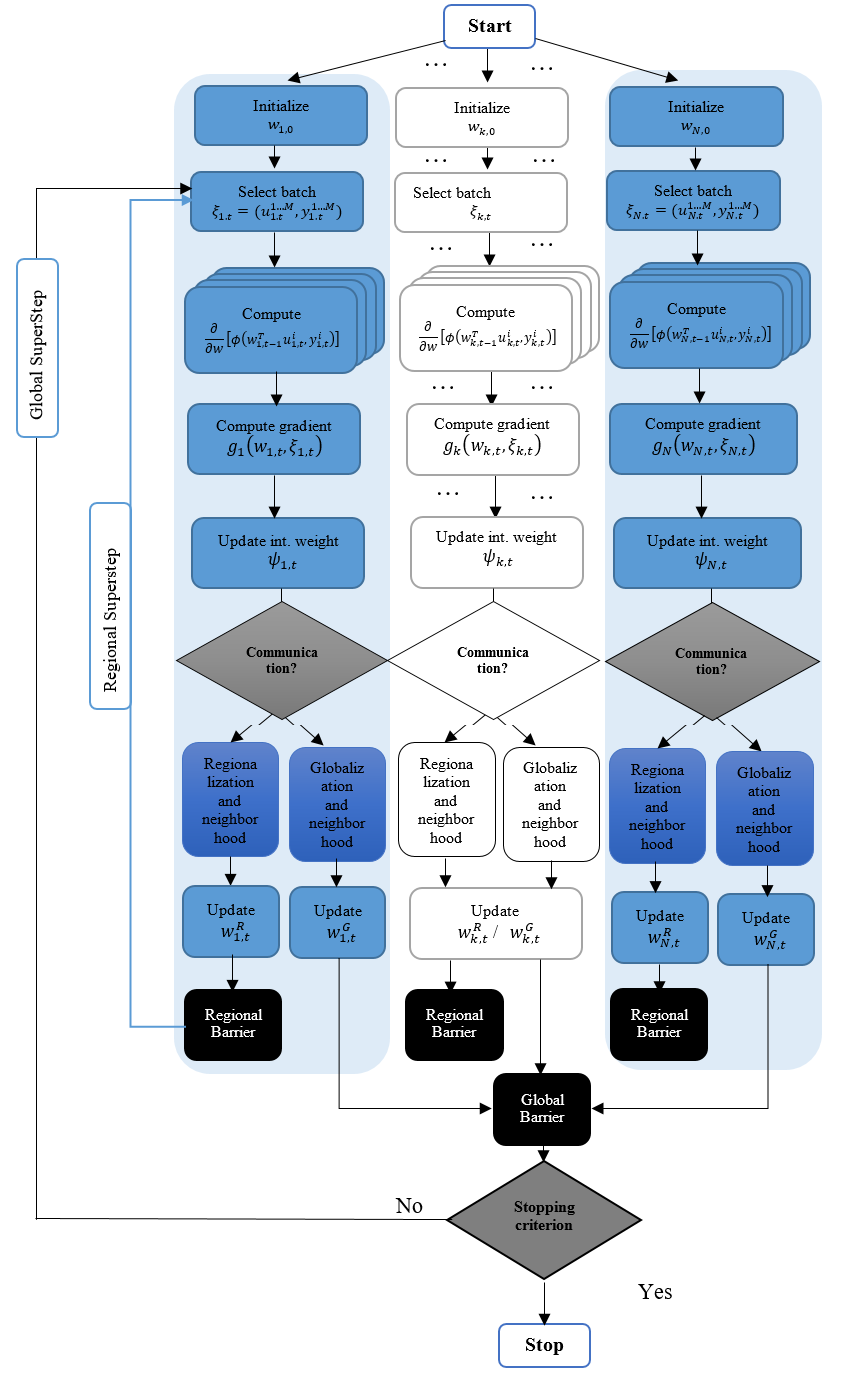
\includegraphics[scale=0.6]{Flow1.png}
		\caption{رفتار شماتیکی مرحله برخط رویکرد پیشنهادی مبتنی بر مدل محاسباتی توسعه یافته \lr{BSP} فدرالی}
		\label{p16}
	\end{center}
\end{figure}

بعد از محاسبه گرادیان محلی و به‌روزرسانی بردار پارامتر میانی، هر گره در مورد نوع ارتباط با گره‌های همسایه‌اش در شبکه باید تصمیم‌گیری نماید. در صورت انتخاب ارتباط منطقه‌ای با گره‌های همسایه، بردار پارامتر به صورت منطقه‌ای با بردارهای پارمتر همسایه‌ها در همان منطقه ترکیب و سپس به‌روزرسانی می‌گردد. در انتهای هر تکرار منطقه‌ای، یک همگام‌سازی مانعی منطقه‌ای نیز باید اجرا گردد. این مراحل یک ابرگام منطقه‌ای در مدل محاسباتی \lr{BSP} فدرالی را تشکیل می‌دهند. اگر گره ارتباط سراسری را انتخاب کند، بردار پارامتر به صورت سراسری با بردارهای پارامتر همسایه‌ها در کل شبکه ترکیب و سپس به‌روزرسانی می‌گردد. در انتهای هر تکرار سراسری، یک همگام‌سازی مانعی سراسری نیز باید اجرا گردد. این مراحل یک ابرگام سراسری در مدل محاسباتی \lr{BSP} فدرالی را تشکیل می‌دهند. این مرحله از رویکرد پیشنهادی کمک می‌کند تا یک پیاده‌سازی موازی غیرهمگام در شبکه‌های تطبیقی توزیع‌شده داشته باشیم. 


با فرض داشتن یک شبکه کوچک کاملا متصل شامل 5 گره با قدرت‌های پردازشی متفاوت، تفاوت زمان‌های انتظار گره‌های کند و سریع و مساله کندکننده‌ها به وضوح در دو حالت اعمال همگام‌سازی مانعی سراسری و همگام‌سازی مانعی منطقه‌ای که به ترتیب در شکل‌های \ref{p18-1} و \ref{p18-2} نشان داده شده است. در شکل \ref{p18-1} گره \lr{C} که سریع‌ترین گره از لحاظ قدرت پردازشی است، مدت زیادی باید منتظر بماند تا عملیات محاسباتی در کندترین گره به پایان برسد. در حالیکه در شکل \ref{p18-2} که همگام‌سازی مانعی منطقه‌ای اعمال شده است، مدت زمان انتظار گره \lr{C} کاهش می‌یابد. در نتیجه مجموع زمان انتظار در کل شبکه نیز در هر بار اجرای همگام‌سازی مانعی کاهش خواهد یافت. همچنین در مدت زمان مشخص، توان عملیاتی و کار انجام شده توسط رویکرد پیشنهادی با روش منطقه‌بندی بیشتر است. در حالتی‌که هیچ منطقه‌بندی در شبکه اجرا نشود، کار انجام شده به اندازه سه ابرگام سراسری است. در مقابل در همان مدت زمان، در حالتی‌که منطقه‌بندی در شبکه اجرا شود، کار انجام شده در یک منطقه به اندازه سه ابرگام و در منطقه دیگر به اندازه 5 ابرگام است.

\begin{figure*}[ht]
	\centering
	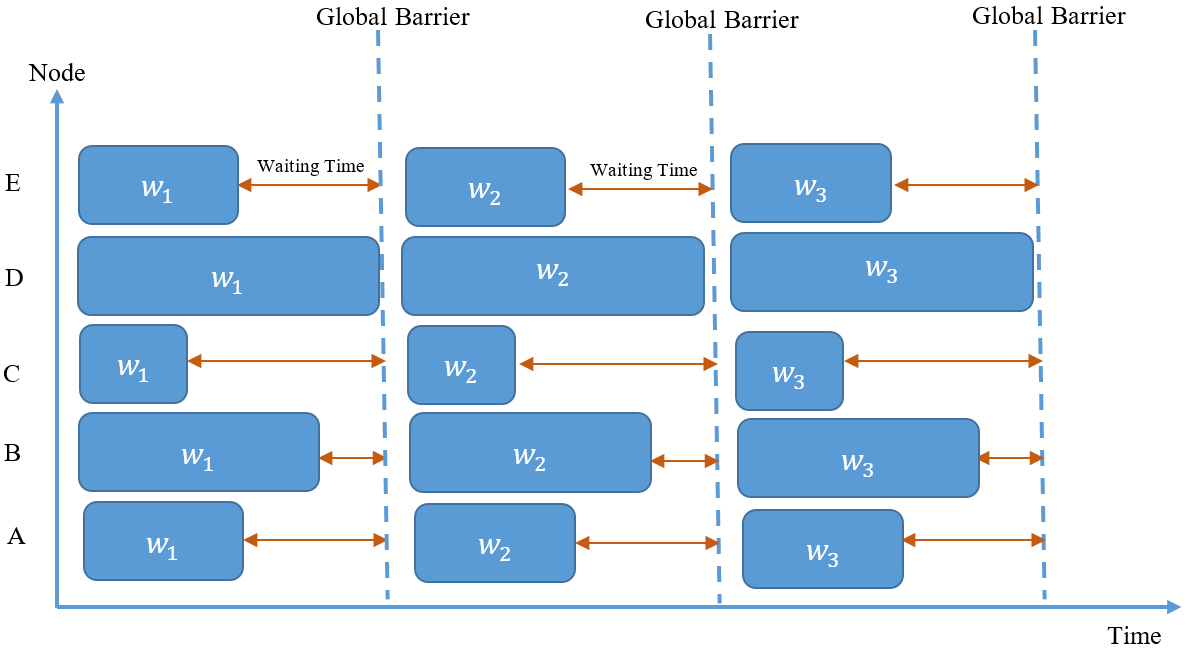
\includegraphics[width=.8\linewidth]{Pic20.PNG}  
	\caption{همگام‌سازی مانعی سراسری و تاثیر آن بر زمان انتظار کل شبکه}
	\label{p18-1}
\end{figure*}

\begin{figure*}[ht]
	\centering 
	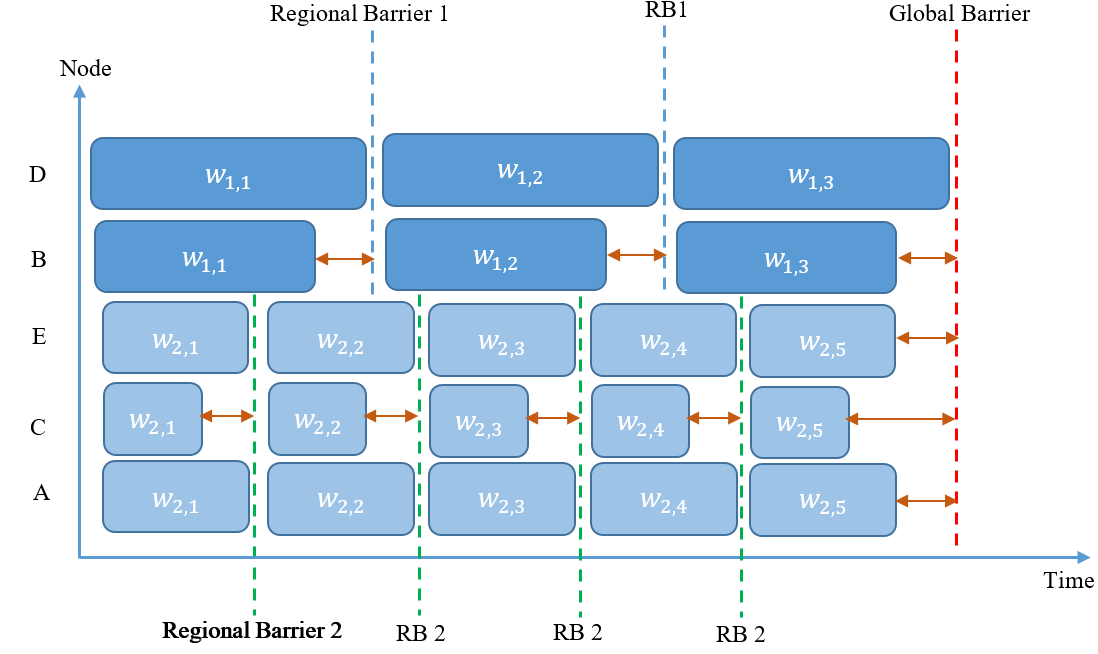
\includegraphics[width=.8\linewidth]{Pic21.PNG}  
	\caption{همگام‌سازی مانعی منطقه‌ای و تاثیر آن بر زمان انتظار کل شبکه}
	\label{p18-2}
\end{figure*}

شکل \ref{p20-2} مراحل اجرای مدل محاسباتی \lr{BSP} فدرالی از دیدگاه گره \lr{N1} در شبکه منطقه‌بندی شده \ref{p20-1} را نشان می‌دهد. ارتباطات گره \lr{N1} با همسایگانش با یال‌های نارنجی رنگ مشخص شده‌اند. در حالت ارتباط منطقه‌ای گره \lr{N1} با گره‌های \lr{N2 } و \lr{N3 } ارتباط برقرار می‌کند و با دریافت بردارهای وزن میانی گره‌های مذکور و ترکیب آنها بردار وزن $w_{1t}^R$ خود را به صورت منطقه‌ای به‌روزرسانی می‌کند و سپس همگام‌سازی مانعی منطقه‌ای اجرا خواهد شد. بعد از اجرای چندین ابرگام منطقه‌ای و احراز شرایط اجرای ارتباط سراسری، گره \lr{N1 } با گره‌های \lr{N2}، \lr{N3}، \lr{N4} و \lr{N5} ارتباط برقرار می‌کند و با دریافت بردارهای وزن میانی گره‌های مذکور و ترکیب آنها اقدام به به‌روزرسانی بردار وزن $w_{1t}^G $ خود به صورت سراسری می‌کند و سپس همگام‌سازی مانعی سراسری اجرا خواهد شد.
\begin{figure*}[ht]
	\centering
	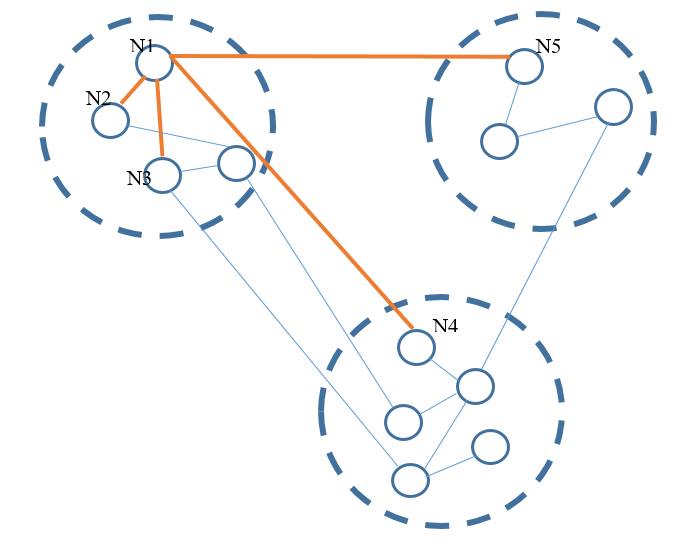
\includegraphics[width=.6\linewidth]{Pic22.PNG}  
	\caption{یک شبکه منطقه‌بندی‌شده}
	\label{p20-1}
\end{figure*}

\begin{figure*}[ht]
		\centering
		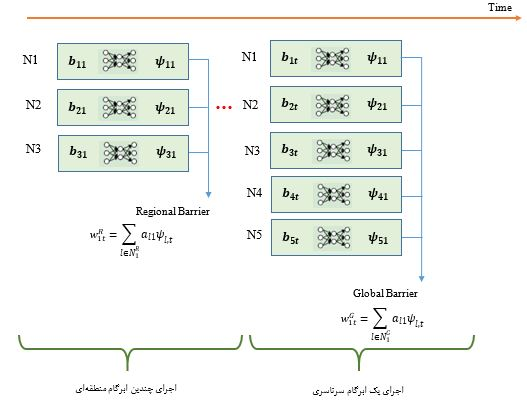
\includegraphics[width=1\linewidth]{Pic23.PNG}
		\caption{مثالی از نحوه اجرای ارتباطات و همگام‌سازی مانعی منطقه‌ای و  سراسری در شبکه \ref{p20-1}}
	\label{p20-2}
\end{figure*}

\subsection{مدل سیستم و فرمول‌بندی مساله}
	در این بخش مدل کلی سیستم یادگیری توزیع‌شده، تابع هدف و فرضیاتی که بر روی تابع هدف در نظر گرفته شده است را تعریف می‌کنیم. 
	در یک سیستم یا به عبارتی در یک شبکه از گره‌ها، مجموعه‌ای‌ از منطقه‌ها به نام \lr{$\mathcal{R}$} تعریف می‌شود که $\mathcal{R}=\{1,...,R\}$ است. هر منطقه $r\in \mathcal{R}$ شامل مجموعه‌ای از گره‌ها $M^{(r)}$ است که $|M^{(r)}|=N^{(r)}$. مجموعه تمام گره‌ها در کل شبکه به صورت $M=\bigcup_{r=1}^R M^{(r)}$ تعریف می‌شود. گره‌ها از طریق یک گراف ارتباطی متصل غیرجهت‌‌دار $G=(M,E)$ با یکدیگر در ارتباط می‌باشند. هر گره $i$ یک مجموعه داده آموزشی محلی $U^{(i)}$ دارد که کل مجموعه داده‌های آموزشی سیستم به صورت $U=\bigcup_{i=1}^N U^{(i)}$ تعریف می‌شود.  
	
	فرض کنید $N_i=\{j|e_{ij}\in E\}$ مجموعه همسایگی گره $i$ در گراف $G$ و $N_i^{(r)}=\{j| e_{ij}\in E\quad and\quad j\in M^{(r)}\}$ مجموعه همسایگی گره $i$ در منطقه $r$ است. هر گره $i\in M^{(r)}$ می‌تواند با هر گره‌ همسایه $ k$ در منطقه $r$ ($k\in N_i^{(r)}$) و هر گره همسایه $j$ در شبکه $G$ ($j\in N_i$) ارتباط برقرار کند. 
  
	
	همان‌طور که قبلا بیان شده است، $w\in R^{M\times 1}$ بردار وزن یا بردار پارامترها نامیده می‌شود و هدف ما پیدا کردن $w$ است به گونه‌ای که تابع هدف زیر بر روی مجموعه داده‌های آموزشی مورد نظر کمینه گردد:
\begin{equation}
	J(w)=\frac{1}{|U|}\sum_{U^i\in U} J_i(w,U^i)
\end{equation}
	
که $J_i(.)$ تابع زیان است. هر گره‌ با همکاری سایر گره‌های همسایه خود سعی در کمینه کردن این تابع زیان با استفاده از مجموعه داده‌های آموزشی محلی خود دارد. 
	
	در هر تکرار، هر گره دسته‌ای از داده‌های آموزشی محلی خود را به صورت تصادفی نمونه‌برداری می‌کند. فرض کنید که $\xi$ دسته نمونه‌برداری شده و $g(w;\xi)=\frac{1}{|\xi|}\sum_{u^i\in \xi} \nabla f(w;u^i)$ گرادیان دسته‌ای است. برای سادگی در ادامه $g(w)$ به جای $g(w;\xi)$ به کاربرده می‌شود.
	
	
\begin{assumption}
	در این رساله فرضیات زیر در مورد تابع هدف و گرادیان دسته‌ای در نظر گرفته شده است:
		\begin{enumerate}\label{Farz1}
		\item \label{F11}
		تابع هدف $J: R^M\rightarrow R$ پیوسته و مشتق‌پذیر است و گرادیان آن از قانون لیپشیتز با ثابت $\delta>0$ پیروی می‌کند که
		\begin{center}
			$||\nabla_{w}J(w_2)-\nabla_{w}J(w_1)||_2<=\delta||w_2-w_1||_2, \qquad for\quad all\quad w_1,w_2\in R^{M\times 1}$
		\end{center}
		این شرط مستلزم این است که گرادیان‌ها خیلی سریع تغییر نکنند. 
		\item \label{F12}
		در حالت کلی تابع هدف $J(w) $ کران پایین دارد. این فرض مستلزم این است که تابع هدف با مقدار $J_{inf} (w)$ از پایین محدود باشد.
		
		\begin{center}
			$J(w)\ge J_{inf}(w)>-\infty \qquad for \quad all \quad w\in R^{M\times 1}$
		\end{center}
		
		\item \label{F13}
		گرادیان‌های دسته‌ای $g(w)$ بی‌طرفانه هستند:	
		\begin{center}
			$E_{\xi|w}[g(w)]=\nabla J(w) \qquad for \quad all \quad w\in R^{M\times 1}$ 
		\end{center} 
		\item \label{F14}
		با فرض اینکه اسکالرهای $\sigma$ و $\beta$ وجود دارند که 
		
		\begin{center}
			$E_{\xi|w} ||g(w)-\nabla J(w)||_2^2\le \beta||\nabla J(w)||_2^2+\sigma^2,\qquad for \quad all \quad w\in R^{M\times 1}$  
		\end{center}
	این فرض شبیه فرض واریانس محدود شده است. در مورد آخر فرض می‌شود که داده‌های محلی در هر گره می‌توانند به عنوان یک تخمین بی‌طرفانه برای مجموعه داده کامل با همان واریانس محدود استفاده شوند. این فرضیات در تحلیل همگرایی الگوریتم‌های گرادیان کاهشی تصادفی رایج و معمول هستند.
\end{enumerate}
\end{assumption}

رابطه به‌روزرسانی استفاده شده در مرحله تطبیق و ترکیب هر گره‌ $K$ و نرخ‌ متفاوت محاسبات (قدرت پردازشی متفاوت) گره‌ها به صورت زیر مدل می‌شود:

\begin{flalign}\label{ATC1}
	&\psi_{k,t}=w_{k,t-1}-\mu_k(t) S_t^{-1}(\lambda\ w_{k,t-1}-\nabla_{w}{J_k(w)})\\
	&w_{k,t}=\sum_{l\in N_k} a_{lk} \psi_{l}(t)\\
	&\mu_k(t)=
	\begin{cases}
		\mu_k\quad with\ a\ probability\ of\ P_k\\
		0\ \quad with\ a\ probability\ of\ 1-P_k
	\end{cases}
\end{flalign} 
که هر گره $k$، از $\tau$ تکرار تنها $\tau^{(k)}$  تکرار را اجرا می‌کند ($\tau^{(k)} \leq \tau$). $P$ یک بردار به طول $N$ است که $P_k=\frac{\tau^{(k)}}{\tau}$ احتمال اینکه گره $k$ یک گام به‌روزرسانی را در هر تکرار اجرا نماید. 

تحلیل ما در این بخش بر چگونگی تکامل مدل‌ گره‌ها متمرکز است. ابتدا یک فرمول معادل از الگوریتم پیشنهادی از نظر تکامل مدل‌ گره‌ها ارائه کرده و سپس نتیجه اصلی را در مورد همگرایی و پایداری الگوریتم خود ارائه می‌کنیم. رفتار سیستم با استفاده از قانون به‌روزرسانی کلی \ref{mo} مدل می‌شود:	

\begin{equation}\label{mo}
	w_t=B(t) w_{t-1}-\mu(t) S_t^{-1}\lambda\ B(t) w_{t-1} +\mu(t)S_t^{-1}\ B(t) G_t
\end{equation}
که $G_t=[\nabla J_1(t), \nabla J_2(t), ..., \nabla J_N(t)]^T$،   $w_t=[w_{1,t},w_{2,t}, ..., w_{N,t}]^T$ و    $B(t)\in R^{N\times N}$ یک عملگر متغیر با زمان است که دو مدل ارتباط سراسری و ارتباط منطقه‌ای در رویکرد پیشنهادی را شامل می‌شود. به منظور مدل کردن رفتار سیستم با یک رابطه به‌روزرسانی کلی، ماتریس $B(t)$ را به صورت زیر تعریف می‌کنیم:
\begin{equation}\label{Bmarix}
	B(t)=
	\begin{cases}
		Z(t)\quad if\ t\ mod \ q=0\\
		V(t)\quad otherwise
	\end{cases}
\end{equation}
در مرحله ارتباطات سراسری که هر گره برای به‌روزرسانی بردار پارامتر خود با همسایگانش در کل شبکه ارتباط برقرار می‌کند، ماتریس مربعی $Z(t)$ به ابعاد $N\times N$ به صورت $Z=A$ در نظر گرفته می‌شود. در مرحله ارتباطات منطقه‌ای که هر گره برای به‌روزرسانی بردار پارامتر خود با همسایگان هم‌منطقه‌اش ارتباط برقرار می‌کند، ماتریس مربعی $V(t)$ به ابعاد $N\times N$ به گونه‌ای تعریف می‌شود که هر درایه این ماتریس، وزن گره‌های همسایه و هم‌منطقه با گره  $i$ را نشان می‌دهد. 
\begin{equation}\label{Nt}
	Z_{i,j}(t)=
	\begin{cases}
		a_{ij}\quad if\ j\in N_i\\
		0 \quad otherwise
	\end{cases},\quad
	V_{i,j}(t)=
	\begin{cases}
		a_{ij}\quad if\ j\in N_i^{(r)}\\
		0 \quad otherwise
	\end{cases}
\end{equation}

فرض کنید $\boldsymbol{\Xi}=\{\xi_1{(t)},...,\xi_N{(t)}\}$ مجموعه دسته داده‌های استفاده شده توسط $N$ عامل در زمان $t$ باشد. بدون از دست دادن کلیت، ما یک دسته داده  به هر عامل اختصاص می‌دهیم، حتی اگر عامل موردنظر در یک تکرار عمل به‌روزرسانی را اجرا نکند. همچنین مجموعه متغیرهای تصادفی برنولی $\boldsymbol{\Theta}=\{\theta_1(t),...,\theta_N(t)\}$ به صورت زیر تعریف می‌شوند: 
\begin{equation}\label{eTheta}
	\theta_i(t)=
	\begin{cases}
		1\qquad with\quad probability\quad p_i\\
		0\qquad with\quad probability\quad (1-p_i)
	\end{cases}
\end{equation}
بر این اساس، می‌توان تعریف معادلی برای گرادیان $g_i(t)$ به صورت زیر ارائه داد: 


\begin{equation}
	g_i(t)=\theta_i(t)g(\xi_i(t))
\end{equation}
در ادامه برای سادگی به جای $E_{\boldsymbol{\Theta}_t,\boldsymbol{\Xi}_t|W_t}$ از معادل آن $E_t$ در روابط استفاده می‌شود. بر اساس فرض \ref{F13} در \ref{Farz1} خواهیم داشت:
\begin{equation}
	E_t[g_i(t)]=p_i E[g(w_i(t))]\\
	=p_i\nabla J(w_i(t))
\end{equation}
و همچنین زمانی‌که $i\ne j$ باشد، خواهیم داشت:

\begin{equation}
	E_t[(g_i(t))^T g_j(t)]=p_i p_j E_t[g(w_i(t))]^T E_t[g(w_j(t))]=p_i p_j \nabla J{(w_i(t))}^T \nabla J(w_j(t))
\end{equation}

بر اساس فرض شماره \ref{F14} در \ref{Farz1} می‌توان نتیجه گرفت که، 
\begin{flalign}
	E_t[\lVert(g_i(t))-&\nabla J(w_i(t))\rVert^2]= E_t[\lVert(g_i(t))\rVert^2+\lVert \nabla J(w_i(t))\rVert^2 -2 (g_i(t))^T \nabla J(w_i(t))]\\
	&=E_t[\lVert(g_i(t))\rVert^2+\lVert \nabla J(w_i(t))\rVert^2 -2 E_t[(g_i(t))]^T \nabla J(w_i(t))]\\
	&=p_i E_t[\lVert(g(w_i(t)))\rVert^2+\lVert \nabla J(w_i(t))\rVert^2 -2 p_i E_t[(g(w_i(t)))]^T \nabla J(w_i(t))]
\end{flalign}

\begin{flalign}
	\begin{split}
		E_t[\lVert(g_i(t))-&\nabla J(w_i(t))\rVert^2]=p_i E_t[\lVert(g(w_i(t)))\rVert^2+ p_i \lVert \nabla J(w_i(t))\rVert^2\\
		&-2 p_i E_t[(g(w_i(t)))]^T \nabla J(w_i(t))]+ (1-p_i) \lVert \nabla J(w_i(t))\rVert^2
	\end{split}\\
	&=p_i E_t[\lVert(g(w_i(t)))-\nabla J(w_i(t))\rVert^2+ (1-p_i) \lVert \nabla J(w_i(t))\rVert^2\\
	&\le p_i \beta \lVert \nabla J(w_i(t))\rVert^2+p_i\sigma^2 + (1-p_i) \lVert \nabla J(w_i(t))\rVert^2\\
	&= (p_i (\beta-1)+1) \lVert \nabla J(w_i(t))\rVert^2+p_i\sigma^2
\end{flalign}
	

\section{الگوریتم رویکرد یادگیری پیشنهادی}
الگوریتم \ref{Alg_Proposed} شبه‌کد کلی بخش یادگیری رویکرد پیشنهادی را نشان می‌دهد. هر گره یک کپی از مدل یا همان بردار پارامترها را در اختیار دارد. گره‌ها در هر منطقه به صورت موازی و مستقل از سایر منطقه‌های شبکه آموزش می‌بینند و مدل خود را با کمک گره‌های همسایه در منطقه خود به‌روزرسانی می‌کنند. همچنین، گره‌ها قادر هستند مدل خود را با کمک گره‌های همسایه در کل شبکه به صورت دوره‌ای به‌روزرسانی کنند.
\begin{latin}
	\begin{algorithm}
	\caption{ The algorithm of proposed approach}\label{Alg_Proposed}
	\begin{algorithmic}[1]
		\State Initialize $ w_{l}(0)=0$ for $l\in\{1,2,...,N\}$
		\State Given non-negative real coefficients \{$a_{lk}$\}
		\State Given suitable step-size parameter $\mu_t>0$
		\For {$t\in\{1,2,...,T\}$}
		\For  {$r\in  \mathcal{R}$} 
		\For {$k\in M^{(r)}$}
		\For {$j\in \{t, t+1, ..., t+\tau-1\}$}
		\State $\psi_{k,t}=w_{k,t-1}-\mu_k(t) S_t^{-1}(\lambda w_{k,t-1}-\nabla_{w}{J_k(w)})$
		\EndFor
		\If{$t\ mod\ q!=0$}
		\State $w_{k,t}=\sum_{l\in N_k^{(r)}} a_{lk} \psi_{l,t}$
		\Else
		\State $w_{k,t}=\sum_{l\in N_k} a_{lk} \psi_{l,t}$
		\EndIf
		\EndFor
		\EndFor
		\EndFor
	\end{algorithmic}
\end{algorithm}
\end{latin}
	
\section{تجزیه و تحلیل نظری الگوریتم پیشنهادی}
با تمرکز بر جنبه‌های عددی الگوریتم \lr{DSGD}، برای تحلیل و اثبات همگرایی الگوریتم یادگیری پیشنهادی از شیوه ارائه شده در مقاله \cite{Zin2010} که برای الگوریتم‌های گرادیان کاهشی تصادفی مرتبه دوم است، الهام گرفته شده است و همچنین از سنجه جدید اختلاف همگرایی وزنی \footnote{\lr{the weighted convergence difference}} استفاده شده است. این سنجه با استفاده از رابطه \ref{DeltaW} تعریف می‌شود. 

\begin{equation}\label{DeltaW}
	\Delta(w_{k,t},w_{k,t-1},w)=R_{w,t,k}-R_{w,t-1,k}=\lvert\lvert w_{k,t}-w\rvert\rvert^2_S-\lvert\lvert w_{k,t-1}-w\rvert\rvert^2_S
\end{equation}

در این بخش همگرایی الگوریتم یادگیری پیشنهادی در حالت کلی و بدون در نظر گرفتن یک تابع زیان خاص مورد بررسی قرار می‌گیرد. برای سادگی $\phi^{'}(w_{k,t}^T u_{k,},y_{k,t})$ به صورت مختصر با $\phi^{'}_{k,t}$ نمایش داده می‌شود. همان طور که ذکر شد، سنجه اختلاف همگرایی وزنی اساس تحلیل ما است و به صورت زیر تجزیه می‌شود:

\begin{equation}\label{decompositionF}
	\begin{split}
		&\Delta(w_{k,t},w_{k,t-1},w)=\\
		& \lvert\lvert\sum_{l\in N_k} a_{lk}w_{l,t-1}-\mu_{t} S^{-1} \sum_{l\in N_k} a_{lk}\left(\phi^{'}_{l,t}u_{l,t}+\lambda w_{l,t-1}\right)-w\rvert\rvert^2_S-\\
		&\lvert\lvert\sum_{l\in N_k} a_{lk}w_{l,t-2}-\mu_{t-1} S^{-1} \sum_{l\in N_k} a_{lk}\left(\phi^{'}_{l,t-1}u_{l,{t-1}}+\lambda w_{l,t-2}\right)-w\rvert\rvert^2_S
	\end{split}
\end{equation}

که 

\begin{equation}\label{decomposition}
	\begin{split}
		&\Delta(w_{k,t},w_{k,t-1},w)=\lvert\lvert\sum_{l\in N_k} a_{lk}w_{l,t-1}-w\rvert\rvert^2_S+\\
		&\mu^2_t \lvert\lvert\sum_{l\in N_k} a_{lk}\phi^{'}_{l,t}u_{l,t}+\lambda \sum_{l\in N_k} a_{lk} w_{l,t-1}\rvert\rvert^2_{S^{-1}}-\\
		&2\mu_t \left(\sum_{l\in N_k} a_{lk}w_{l,t-1}-w\right)^T\left(\sum_{l\in N_k} a_{lk}\phi^{'}_{l,t}u_{l,t}+\lambda \sum_{l\in N_k} a_{lk} w_{l,t-1}\right)\\
		&-\lvert\lvert\sum_{l\in N_k} a_{lk}w_{l,t-2}-w\rvert\rvert^2_S+2\mu_{t-1}\left(\sum_{l\in N_k} a_{lk}w_{l,t-2}-w\right)^T\\
		&\left(\sum_{l\in N_k} a_{lk}\phi^{'}_{l,t-1}u_{l,t-1}+\lambda \sum_{l\in N_k} a_{lk} w_{l,t-2}\right)\\
		&-\mu^2_{t-1}\lvert\lvert\sum_{l\in N_k} a_{lk}\phi^{'}_{l,t-1}u_{l,{t-1}}+\lambda \sum_{l\in N_k} a_{lk} w_{l,t-2}\rvert\rvert^2_{S^{-1}}
	\end{split}
\end{equation}
در هر تکرار $t$، بردار پارامترهای بدست آمده $w_{k,t}$ باید نسبت به بردار پارامترهای تکرار قبلی $w_{k,t-1}$، به بردار پارامترهای بهینه $w$ نزدیک‌تر شود. برای خلاصه‌سازی تجزیه بدست آمده در \ref{decomposition}، جملات $\lvert\lvert\sum_{l\in N_k} a_{lk}w_{l,t-1}-w\rvert\rvert^2_S+\mu^2_t \lvert\lvert\sum_{l\in N_k} a_{lk}\phi^{'}_{l,t}u_{l,t}+\lambda \sum_{l\in N_k} a_{lk} w_{l,t-1}\rvert\rvert^2_{S^{-1}}$ و $||\sum_{l\in N_k} a_{lk}w_{l,t-2}-w||^2_S+\mu^2_t||\sum_{l\in N_k} a_{lk}\phi^{'}_{l,t-1}u_{l,{t-1}}+\lambda \sum_{l\in N_k} a_{lk} w_{l,t-2}||^2_{S^{-1}}$ به ترتیب با $A^2$ و $B^2$, نمایش داده می‌شوند. 
\begin{theorem}
	با فرض استقلال نمونه‌های یادگیری $<u_{k,t},y_{k,t}>k=1,...,N, t=1,...,T$ و ثابت بودن اندازه گام‌ها در تکرارهای مختلف $\mu_{t}=\mu$ و $\lambda\ge0$، با استفاده از تجزیه انجام شده در \ref{decomposition} و تعریف سنجه اختلاف همگرایی وزنی داریم:
	\begin{equation}\label{inequality}
		\begin{split}
			&\Delta(w_{k,t},w_{k,t-1},w)\leq A^2-\\
			&2\mu (\lambda \left[\lVert\sum_{l\in N_k} a_{lk}w_{l,t-1}-\frac{1}{2}w\rvert\rvert^2_2-\lvert\lvert\sum_{l\in N_k} a_{lk}w_{l,t-2}-\frac{1}{2}w\rvert\rvert^2_2\right]\\
			&+[\left(\sum_{l\in N_k}a_{l,k}\phi^{'}_{l,t}u_{l,t}\right)^T\left(\sum_{l\in N_k}a_{l,k}w_{l,t-1}-w\right)\\
			&-\left(\sum_{l\in N_k}a_{l,k}\phi^{'}_{l,t-1}u_{l,t-1}\right)^T\left(\sum_{l\in N_k}a_{l,k}w_{l,t-2}-w\right)])
		\end{split}
	\end{equation}
	
\end{theorem}

\begin{proof}
	با مرتب‌سازی جملات در رابطه \ref{inequality} و اعمال تغییر نام‌های مورد نظر، رابطه زیر را می‌توانیم بدست آوریم:
	\begin{equation}\label{Eq12}
		\begin{split}
			&\Delta(w_{k,t},w_{k,t-1},w)=A^2-B^2-\\
			&2\mu\lambda \left[\lVert\sum_{l\in N_k} a_{lk}w_{l,t-1}-\frac{1}{2}w\rvert\rvert^2_2-\lvert\lvert\sum_{l\in N_k} a_{lk}w_{l,t-2}-\frac{1}{2}w\rvert\rvert^2_2\right]\\
			&-2\mu\left(\sum_{l\in N_k}a_{l,k}\phi^{'}_{l,t}u_{l,t}\right)^T\left(\sum_{l\in N_k}a_{l,k}w_{l,t-1}-w\right)\\
			&+2\mu\left(\sum_{l\in N_k}a_{l,k}\phi^{'}_{l,t-1}u_{l,t-1}\right)^T\left(\sum_{l\in N_k}a_{l,k}w_{l,t-2}-w\right)
		\end{split}	
	\end{equation}
	جملات با ضرایب $2\mu\lambda$ و $2\mu$ در \ref{Eq12} را می‌توان به ترتیب با $D$ و $E$ نام‌گذاری و خلاصه کرد و رابطه 
	\begin{equation}\label{equality}
		\Delta(w_{k,t},w_{k,t-1},w)=A^2-B^2-2\mu\lambda D-2\mu E
	\end{equation}
	را بدست آورد. به وضوح مشخص است که جمله $B^2$  غیرمنفی است. بر این اساس، رابطه \ref{equality} به صورت نامساوی \ref{inequality2} بازنویسی می‌شود. این نامساوی نتیجه مهم این تحلیل است. 
	\begin{equation}\label{inequality2}
		\Delta(w_{k,t},w_{k,t-1},w)\leq A^2-2\mu (\lambda D+ E)
	\end{equation}
\end{proof}

بسته به سرعت تغییر $\Delta(w_{k,t},w_{k,t-1},w)$، تغییر ممکن است به صورت تدریجی یا ناگهانی باشد. تغییر تدریجی $\Delta(w_{k,t},w_{k,t-1},w)$ باعث می‌شود که نرم‌کننده کمتر تحت تأثیر نویز قرار گیرد. در واقع نرم‌کننده تبدیل به یک کاهنده می‌شود و نرخ همگرایی کاهش می‌یابد. فرض کنید $\mu^*=\argminA_{\mu} \Delta(w_{k,t},w_{k,t-1},w)$. به عبارت دیگر، اگر $\mu^{*}$ منجر به کاهش نرخ همگرایی شود، پس $w_t$ کمتر تحت تاثیر نویز قرار می‌گیرد. در طراحی الگوریتم \lr{DSGD}، اگر بخواهیم الگوریتم سریع‌تر به سمت $w$ حرکت کند، پس باید $\mu^*=\argmaxA_{\mu} \Delta(w_{k,t},w_{k,t-1},w)$ باشد. در این حالت $w_t$ شدیدا به نویز حساس خواهد بود. 

با رشد رابطه \ref{ww}، مقدار عبارت $D$ یک مقدار مثبت کوچک می‌شود. همچنین بخش مشابه آن در عبارت $\theta=A^2-B^2$ نیز یک مقدار مثبت کوچک است. در حالت همگرایی، فاصله بین بردار پارامتر $w$ و $w_{t}$  باید کمتر از فاصله بین  $w$ و $w_{t-1}$ باشد. بنابراین، سمت راست رابطه \ref{inequality} منفی است. عبارت $\lambda D+E$ به $\gamma$  تغییر نام داده می‌شود. همیشه $\theta-2\mu \gamma\le 0$ خواهد بود. با فرض تغییر تدریجی بردار پارامترها، همگرایی الگوریتم \lr{DSGD} در صورت برقراری شرط $\mu \le \frac{\theta}{2\gamma}$ صورت می‌گیرد. 
\begin{assumption}\label{assumption0}
	برای دست یافتن به هدف اصلی و سادگی تحلیل، فرضیات زیر بر روی توابع خطا در نظر گرفته می‌شوند:
	\begin{itemize}
		\item تابع زیان $\phi(\hat{y},y)$ محدب است
		\item ثوابت غیرمنفی $A$ و $B$ به گونه‌ای وجود دارند که $(\phi^{'}(\hat{y},y))^2\leq A\phi(\hat{y},y)+B$
	\end{itemize} 
\end{assumption}

توابع زیانی از جمله هابر، حداقل مربع خطا و ... این فرض را ارضا می‌کنند. به عنوان مثال تابع زیان حداقل مربعات خطا $\phi(\hat{y},y)=(\hat{y}-y)^2$ در حل مساله رگرسیون با انتخاب  $A=4$ و $B=0$  فرض موجود در \ref{assumption0} را ارضا می‌کند. 
برای تحلیل همگرایی الگوریتم \lr{DSGD}،  $\lambda=0$  انتخاب می‌شود. اگر $t\rightarrow\infty$، مساله به کمترین ریسک و خطا همگرا خواهد شد. کران همگرایی به طور مستقیم از نتایج رابطه \ref{inequality} حاصل می‌شود. 

\begin{assumption}\label{Assumption00}
	به منظور تحلیل نرخ همگرایی الگوریتم یادگیری، فرض $\sup\lvert\lvert u_{k,t}\rvert\rvert_{S^{-1}}\leq M$ بر روی هر نمونه داده و برای هر $k=1, 2, ..., N$ و $t=1, 2, ..., T$ در نظر گرفته می‌شود. 
\end{assumption}

\begin{theorem}\label{Theorem00}
	در صورت برقراری فرضیات \ref{assumption0} و \ref{Assumption00} بر روی توابع خطا و نمونه‌های داده، همچنین برای هر گره $k$ در تکرار $t$ فرض می‌کنیم که $\lvert a_{l,k}\rvert\leq L$ برقرار است، پس
	\begin{equation}\label{eq6}
		\begin{split}
			&\Delta(w_{k,t},w_{k,t-1},w)\leq \\
			&\lvert\lvert \sum_{l\in N_k}{a_{l,k}w_{l,t-1}-w} \rvert\rvert^2_S+\mu^2_t \left[(A\sum_{l\in N_k}\phi_{l,t} +B)N_kM^2L^2\right]\\
			&-2\mu_t M\left[(\sum_{l\in N_k}a_{l,k}\phi^{'}_{l,t})^T(\sum_{l\in N_k}a_{l,k}w_{l,t-1}-w)\right]\\
			&+2\mu_t M\left[(\sum_{l\in N_k}a_{l,k}\phi^{'}_{l,t-1})^T(\sum_{l\in N_k}a_{l,k}w_{l,t-2}-w)\right]
		\end{split}
	\end{equation}
\end{theorem}

\begin{proof}
	همان‌طور که قبلا اشاره شد، ضرایب $a_{lk}$ وزن‌های غیرمنفی هستند که شرط در \ref{condition} را ارضا می‌کنند. در نتیجه، $0\leq L\leq 1$ است. برای یافتن یک کران برای جمله دوم $A^2$ در سمت راست رابطه \ref{inequality}، از نامساوی \lr{Cauchy–Schwarz} که به صورت $(\sum x_i y_i)^2\leq \sum x_i^2 \sum y_i^2$ است، استفاده می‌کنیم. بنابراین، می‌توان این جمله را به صورت نامساوی زیر ساده کرد: 
	\begin{equation*}
		\begin{split}
			\lVert\sum_{l\in N_k} a_{lk}\phi^{'}_{l,t}u_{l,t}\rvert\rvert^2&\leq \sum_{l\in N_k}\lvert\lvert a_{l,k}\phi^{'}_{l,t}\rvert\rvert^2 \sum_{l\in N_k}\lvert\lvert u_{l,t}\rvert\rvert^2\\
			&\leq N_k M^2 L^2\sum_{l\in N_k}\lvert\lvert \phi^{'}_{l,t}\rvert\rvert^2\\
			&\leq N_k M^2 L^2(A\sum_{l\in N_k}\phi_{l,t}+B)
		\end{split}
	\end{equation*}
	که $N_k$ مجموعه همسایگی گره $k$ است. جمله $D$ به دلیل $\lambda=0$ حذف خواهد شد. یک کران برای جمله $E$ در رابطه \ref{inequality} بر اساس نامساوی \lr{Cauchy–Schwarz} به صورت زیر بدست می‌آید:
	\begin{equation*}
		\begin{split}
			E&\leq M\left[(\sum_{l\in N_k}a_{l,k}\phi^{'}_{l,t})^T(\sum_{l\in N_k}a_{l,k}w_{l,t-1}-w)\right]\\
			&-M\left[(\sum_{l\in N_k}a_{l,k}\phi^{'}_{l,t-1})^T(\sum_{l\in N_k}a_{l,k}w_{l,t-2}-w)\right]
		\end{split}
	\end{equation*}
\end{proof}

قضیه \ref{Theorem00} یک کران بالا برای خطا تولید شده توسط رابطه به‌روزرسانی بردار پارامترها نتیجه می‌دهد و نشان می‌دهد که همگرایی الگوریتم \lr{DSGD} وابسته به پارامتر اندازه گام $\mu$ است. 

به منظور سادگی بحث، جملات سمت راست رابطه \ref{inequality}، به $A_c=N_kM^2L^2(A\sum_{l\in N_k}\phi_{l,t} +B)$،   $B_c=M[(\sum_{l\in N_k}a_{l,k}\phi^{'}_{l,t})^T(\sum_{l\in N_k}a_{l,k}w_{l,t-1}-w)-(\sum_{l\in N_k}a_{l,k}\phi^{'}_{l,t-1})^T(\sum_{l\in N_k}a_{l,k}w_{l,t-2}-w)]$ و $C_c=\lvert\lvert \sum_{l\in N_k}{a_{l,k}w_{l,t-1}-w} \rvert\rvert^2_S$ تغییر نام داده می‌شوند. 

\begin{theorem}
	با فرض تغییرات تدریجی بردارهای پارامتر هر گره $k$ در هر تکرار $t$ و تحت تاثیر فرضیات \ref{assumption0} و \ref{Assumption00} و $\mu_t=\mu>0$، پارامتر اندازه گام الگوریتم یادگیری \lr{DSGD} در بازه زیر اعمال می‌شود: 
	\begin{equation}\label{cond_eta}
		\frac{B_c-\sqrt{B_c-A_cC_c}}{A_c}<\mu_t<\frac{B_c+\sqrt{B_c-A_cC_c}}{A_c}
	\end{equation}
\end{theorem}

\begin{proof}
	سمت راست رابطه \ref{inequality} به صورت $f(\mu)=A_c\mu^2 -2\mu B_c+C_c$ بازنویسی می‌شود که این رابطه یک معادله درجه دوم با متغیر نامشخص $\mu$ و ضرایب مشخص $A_c$، $B_c$ , $C_c$ است. به منظور همگرا شدن الگوریتم، این معادله باید غیرمثبت باشد.
	\begin{equation}\label{fmu}
		A_c\mu^2 -2\mu B_c+C_c\leq 0
	\end{equation}
	غیرمنفی بودن $A_c$ و $C_c$ واضح است. پس لازم است بر روی $B_c$ برای تعیین علامت معادله درجه دوم بحث کنیم. اگر $B_c<0$ و $\Delta=4B_c^2-4A_cC_c<0$ یا $\Delta=0$ باشد، علامت معادله درجه دو مشابه علامت $A_c$ است. همان طور که قبلا اشاره شده است، $A_c$ همیشه غیرمنفی است که بر خلاف شرط مورد نظر برای همگرایی است. اگر $\Delta>0$ باشد، علامت معادله درجه دوم بین دو ریشه $\mu_1=\frac{B_c-\sqrt{B_c-A_cC_c}}{A_c}$ و  $\mu_2=\frac{B_c+\sqrt{B_c-A_cC_c}}{A_c}$ مخالف علامت $A_c$ است. طبق فرض $B_c<0$،  شرط \ref{cond_eta}  برای دستیابی به همگرایی باید ارضا شود. همانطور که قبلاً فرض کردیم، پارامتر اندازه گام $\mu>0$ است. بنابراین، 
	\begin{equation}
		0<\mu<\frac{B_c+\sqrt{B_c-A_cC_c}}{A_c}
	\end{equation}
	
\end{proof}

همانطور که در این بخش دیده شد، همگرایی الگوریتم یادگیری توزیع‌شده پیشنهادی در حالت کلی و بدون در نظر گرفتن تابع زیان مشخصی بررسی و اثبات شد. تابع زیان یک تابع ریاضی است که تفاوت بین مقادیر پیش‌بینی شده توسط الگوریتم یادگیری و مقادیر واقعی را کمینه‌سازی می‌کند. در واقع عملکرد الگوریتم یادگیری را اندازه‌گیری می‌کند و فرآیند بهینه‌سازی را با ارائه بازخورد در مورد میزان نزدیکی جواب با داده‌ها هدایت می‌کند. توابع خطا مختلفی تا کنون ارائه شده است که هر یک ویژگی‌ها و قابلیت‌های متفاوتی دارد. 

\section{تجزیه و تحلیل نظری رویکرد پیشنهادی}
به منظور تجزیه و تحلیل کارایی رویکرد پیشنهادی، بردار گرادیان \ref{deriv_Jk} بر اساس دو جمله اول سری مک‌لوران به صورت زیر  تقریب زده می‌شود:

\begin{equation}\label{grad_j}
	\nabla J_k(w)\cong-u_{k,t}^T e_k(t)+ \frac{1}{\delta^2}u_{k,t}^T e_k^3(t)
\end{equation}
بردارهای وزن خطای محلی هر گره $k$ به صورت \ref{WEV} تعریف می شوند:

\begin{flalign}\label{WEV}
	&\tilde{w}_{k,t}=w_o-w_{k,t}\\
	&\tilde{\boldsymbol{\psi}}_{k,i}=w^o-\boldsymbol{\psi}_{k,i}
\end{flalign}

با جایگذاری مدل در نظر گرفته شده برای سیگنال مطلوب $d_k(t)$ (\ref{modelee}) در رابطه بردار خطا تخمین $e_k(t)=d_{k,t}-w_{k,t-1}^T u_{k,t}$ و در نظر گرفتن \ref{WEV}، تعریف $e_k(t)$ به صورت زیر بازنویسی می‌شود:

\begin{equation}\label{e_k}
	\begin{split}
		e_k(t)&=u_{k,t}^T(w_o-w_{k,t-1})+\nu_k(t)\\
		&=u_{k,t}^T \tilde{w}_{k,t-1}+\nu_k(t)
	\end{split}
\end{equation}
جمله $e_k^3(t)$ در \ref{grad_j} بر اساس عبارت $e_k(t)e^2_k(t)$ و \ref{e_k} به صورت \ref{e3} نوشته می‌شود.
\begin{equation}\label{e3}
	\begin{split}
		e_k^3(t)&=(u_{k,t}^T\tilde{w}_{k,t-1})^3+3\nu_k(t)(u_{k,t}^T\tilde{w}_{k,t-1})^2\\
		&+3\nu_k^2(t)(u_{k,t}^T\tilde{w}_{k,t-1})+\nu_k^3(t)
	\end{split}
\end{equation}
با جایگذاری رابطه بدست آمده برای  $e^3_k(t)$ در \ref{grad_j} و در نظر گرفتن بردار وزن خطای محلی در \ref{WEV}، رابطه $\tilde{w}_{k,t}$ به صورت زیر حاصل می شود:
\begin{equation}\label{w_vector}
	\begin{split}
		\tilde{w}_{k,t}&=\sum_{l\in N_{k,t}}b_{lk} \tilde{w}_{k,t-1}-\mu S^{-1}\sum_{l\in N_{k,t}}b_{lk}(u_{k,t}u^T_{k,t}\tilde{w}_{k,t-1})\\
		&-\mu S^{-1} \sum_{l\in N_{k,t}}b_{lk} u^T_{k,t} \nu_k(t)\\
		&+\mu S^{-1}\frac{a}{2\delta^2}\sum_{l\in N_{k,t}}b_{lk}  u^T_{k,t}\{(u_{k,t}^T\tilde{w}_{k,t-1})^3+3\nu_k(t)(u_{k,t}^T\tilde{w}_{k,t-1})^2
		\\
		&+3\nu_k^2(t)(u_{k,t}^T\tilde{w}_{k,t-1})+\nu_k^3(t)\}+\mu \lambda S^{-1} \sum_{l\in N_{k,t}}b_{lk} w_{k,t-1}
	\end{split}
\end{equation}
که مجموعه همسایگی $N_{k,t}$ با توجه به رابطه \ref{Nt} و مقدار $t$  توسط یکی از مجموعه های $N_k$ یا $N_k^{(r)}$ مقداردهی می‌شود. $b_{lk}$ درایه $lk$ ماتریس $B(t)$  است. به منظور سادگی تحلیل رویکرد پیشنهادی، تعریف بردارها و ماتریس‌های زیر را خواهیم داشت: 
\begin{flalign}\label{Q1}
	&\mathcal{R}_{k,t} \overset{\Delta}{=}  u_{k,t}^T u_{k,t}\\
	&\mathcal{G}_{k,t} \overset{\Delta}{=}  u_{k,t}^T \nu_k(t)\\
	&\mathcal{P}^{'}_{k,t} \overset{\Delta}{=}  u_{k,t}^T (u_{k,t}^T \tilde{w}_{k,t-1})^3\\
	&\mathcal{Q}^{'}_{k,t} \overset{\Delta}{=}  \nu_k(t) u_{k,t} (u_{k,t}^T \tilde{w}_{k,t-1})^2\\
	&\mathcal{H}_{k,t} \overset{\Delta}{=} \nu_k(t) u_{k,t}^T u_{k,t}\\
	&\mathcal{S}_{k,t} \overset{\Delta}{=} \nu^2_k(t) u_{k,t}^T u_{k,t}\\
	&\mathcal{T}_{k,t} \overset{\Delta}{=}  u_{k,t}^T \nu^3_k(t)	
\end{flalign}
هنگامی که $t\to \infty$، $\mathcal{Q}^{'}_{k,t}$ و $\mathcal{P}^{'}_{k,t}$ می‌توانند به صورت زیر تقریب‌زده شوند:
\begin{flalign}\label{Q2}
	&\mathcal{P}_{k,t} \overset{\Delta}{=}  u_{k,t}^T (u_{k,t}^T \tilde{w}_{k,t-1})=\mathcal{R}_{k,t} \tilde{w}_{k,t-1}\\
	&\mathcal{Q}_{k,t} \overset{\Delta}{=}  \nu_k(t) u_{k,t}^T u_{k,t} \tilde{w}_{k,t-1}=\mathcal{H}_{k,t} \tilde{w}_{k,t-1}
\end{flalign}
همچنین بردارها و ماتریس‌های بلوکی به صورت زیر تعریف می‌گردند:
\begin{flalign}\label{Q3}
	&\mathcal{R}_{t} \overset{\Delta}{=}  diag\{\mathcal{R}_{k,t}, k=1,...,N\}\\
	&\mathcal{H}_{t} \overset{\Delta}{=}  diag\{\mathcal{H}_{k,t}, k=1,...,N\}\\
	&\mathcal{S}_{t} \overset{\Delta}{=}  diag\{\mathcal{S}_{k,t}, k=1,...,N\}\\
	&\mathcal{G}_{t} \overset{\Delta}{=}  col\{\mathcal{G}_{k,t}, k=1,...,N\}\\
	&\mathcal{T}_{t} \overset{\Delta}{=}  col\{\mathcal{T}_{k,t}, k=1,...,N\}\label{33}\\
	&\mathcal{M} \overset{\Delta}{=}  diag\{\mu_t I_M S^{-1}, k=1,...,N\}\label{34}
\end{flalign}
بر اساس \ref{34} و \ref{w_vector}، تعاریف $\mathcal{M}^{'}$ و $\mathcal{M}^{''}$ را به صورت زیر خواهیم داشت:
\begin{flalign}\label{E15}
	&\mathcal{M}^{'} \overset{\Delta}{=}  \frac{1}{2\delta^2}\mathcal{M}\\ &\mathcal{M}^{''} \overset{\Delta}{=}  \frac{3}{2\delta^2}\mathcal{M}
\end{flalign}


ماتریس $B$ با استفاده از ضرب کرونکر به صورت $\mathcal{B}=B\otimes I_M$ گسترش می‌یابد و تعریف بردار وزن و بردارهای وزن خطای کلی به صورت زیر ارائه می‌گردند:

\begin{equation}
	\boldsymbol{w}_t=\begin{bmatrix}
		\boldsymbol{w}_{1,t} \\
		\vdots\\
		\boldsymbol{w}_{N,t}\\		
	\end{bmatrix},\quad
	\boldsymbol{\hat{w}}_t=\begin{bmatrix}
		\boldsymbol{\hat{w}}_{1,t} \\
		\vdots\\
		\boldsymbol{\hat{w}}_{N,t}\\		
	\end{bmatrix},\quad
	\boldsymbol{\hat{\psi}}_t=\begin{bmatrix}
		\boldsymbol{\hat{\psi}}_{1,t} \\
		\vdots\\
		\boldsymbol{\hat{\psi}}_{N,t}\\		
	\end{bmatrix}
\end{equation}
که $\hat{\boldsymbol{w}}_{k,t}=w^o-\boldsymbol{w}_{k,t}$ و $\hat{\boldsymbol{\psi}}_{k,t}=w^o-\boldsymbol{\psi}_{k,t}$ است.
بر اساس \ref{w_vector} و روابط \ref{Q1}-\ref{Q3}، بردار وزن خطای کلی به صورت زیر بازنویسی می‌شود:
\begin{equation}\label{totalW}
	\begin{split}
		\tilde{w}_t &= \mathcal{B} \tilde{w}_{t-1}-\mathcal{B}\mathcal{M}\mathcal{R}_t \tilde{w}_{t-1}-\mathcal{B}\mathcal{M} \mathcal{G}_t+ \mathcal{B}\mathcal{M}^{'} \mathcal{R}_t \tilde{w}_{t-1}\\
		&+ \mathcal{B}\mathcal{M}^{''} \mathcal{H}_t \tilde{w}_{t-1} + \mathcal{B}\mathcal{M}^{'} \mathcal{S}_t \tilde{w}_{t-1} +\mathcal{B}\mathcal{M}^{'} \mathcal{T}_t + \mathcal{B}\mathcal{M}\lambda w
		_{t-1}
	\end{split}
\end{equation}
رابطه (\ref{totalW}) چگونگی تکامل بردار وزن خطای شبکه در طول زمان را بیان می‌کند. این رابطه نقطه شروع تحلیل ما خواهد بود. در ادامه کارایی و عملکرد رویکرد پیشنهادی را از نظر رفتار میانگین و مربع میانگین مورد تحلیل و ارزیابی قرار می‌دهیم. فرضیات \ref{Assum} به منظور انجام این تحلیل‌ها در این رساله در نظر گرفته شده‌اند. 

\begin{comment}
	و به منظور ساده‌سازی تحلیل، بردارها و ماتریس‌های زیر را تعریف می‌کنیم:
	\begin{flalign}
		&\mathcal{D}_t=diag\{u_{k,t}^T u_{k,t}, k=1,...,N\}\\
		&\mathcal{G}_t=col\{u_{k,t}^T \nu_k(t), k=1,...,N\}\\
		&\mathcal{M}_t=diag\{\mu_k(t)I_M S^{-1}_t,k=1,...,N\}\\
		&\mathcal{B}_t=B_t\otimes I_M
	\end{flalign}
	سپس از روابط استفاده شده در الگوریتم \ref{Alg_Proposed} نتیجه می‌گیریم که روابط زیر برای بردارهای خطا برقرار است:
	\begin{equation}\label{errorVector}
		\begin{cases}
			\hat{\psi}_t=\hat{w}_{t-1}-\lambda\mathcal{M}_t w_{t-1}+\mathcal{M}_t \mathcal{G}_t-\mathcal{M}_t \mathcal{D}_t \hat{w}_{t-1}\\
			\hat{w}_t=\mathcal{B}_t^T \hat{\psi}_t
		\end{cases}
	\end{equation}
	با جایگذاری $\hat{\psi}_t$ در رابطه مربوط به بردار وزن خطا $\hat{w}_t$ به رابطه بازگشتی زیر دست خواهیم یافت:
	\begin{equation}\label{totalW}
		\hat{w}_t=\mathcal{B}^T_t [I-\mathcal{M}_t \mathcal{D}_t]\hat{w}_{t-1}+ \mathcal{B}^T_t \mathcal{M}_t \mathcal{G}_t-\lambda \mathcal{B}^T_t \mathcal{M}_t w_{t-1}
	\end{equation}
\end{comment}



\begin{assumption}\label{Assum}
	فرضیات استقلال در نظر گرفته شده در این رساله بر روی داده‌های رگرسیون در تحلیل‌های انجام شده به صورت زیر می‌باشند:
	\begin{itemize}\label{Assum2}
		\item 
		نمونه‌های نویز خروجی $\nu_k(t)$  مستقل هستند و به طور یکسان در طول زمان توزیع می‌شوند. به عبارتی، 	
		$\mathbb{E} \nu_k(t)\nu_l(t^{'})=0, \quad \forall k,l, t\ne t^{'}$
		\item 
		بردار داده رگرسیون $u_{k,t}$ و نمونه نویز خروجی $\nu_l(t^{'})$ به ازای تمام $,k,l,t,t^{'}$ مستقل هستند. به عبارتی، 	 
		$\mathbb{E} \nu_k(t)u_{l,t^{'}}=0, \quad k\ne l$
		\item 
		بردارهای داده رگرسیون مستقل هستند و به طور یکسان در طول زمان توزیع می‌شوند. به عبارتی، 	 $\mathbb{E} u_{k,t}^T u_{l,t}=0, \quad k\ne l$
	\end{itemize}
\end{assumption}


\subsection{بررسی کارایی رویکرد پیشنهادی در حالت میانگین}
با در نظر گرفتن فرضیات \ref{Assum2}، برای مطالعه میانگین همگرایی و پایداری رویکرد پیشنهادی، از هر دو طرف رابطه \ref{totalW} امید ریاضی (میانگین وزن‌دار) گرفته می‌شود. سپس با توجه به اینکه  $R_{u,k}=\mathbb{E}u_{k,t}^T u_{k,t}$ است، به رابطه بازگشتی میانگین خطای زیر خواهیم رسید:

\begin{equation}\label{totalEW}
	\mathbb{E}\hat{w}_t=\mathcal{B}(I-\mathcal{M}\mathcal{R}+\mathcal{M}^{'}\mathcal{R}+\mathcal{M}^{''}\mathcal{H}+\mathcal{M}^{'}\mathcal{S})\mathbb{E}\tilde{w}_{t-1}+\mathcal{B}\mathcal{M}\lambda \mathbb{E}w_{t-1}
\end{equation}
که
\begin{flalign}
	&\mathcal{R}=\mathbb{E}\mathcal{R}_t\\
	&\mathcal{H}=\mathbb{E}\mathcal{H}_t\\
	&\mathcal{S}=\mathbb{E}\mathcal{S}_t
\end{flalign}
و با توجه به فرضیات \ref{Assum}، به دلیل استقلال بردار داده رگرسیون و نمونه نویز خروجی $\mathbb{E}\mathcal{G}_t=0$ و $\mathbb{E}\mathcal{T}=0$ است. 

\begin{comment}
	براساس تعریف مدل سیستم \ref{modelee} و جایگذاری $d_k(t)$ در رابطه $e_k(t)$ رابطه بردار خطا به صورت زیر بازنویسی می‌شود: 
	
	\begin{equation}
		e_k(t)=u_{k,t}^T\hat{w}_{k,t-1}+\nu_k(t)
	\end{equation}
\end{comment}


در ادامه قضیه \ref{Theorem1} و اثبات آن آورده شده است. این قضیه پایداری حالت میانگین رویکرد پیشنهادی را تضمین می‌کند و یک فرم بسته برای بایاس وزن نیز ارائه می‌دهد.

\begin{theorem}\label{Theorem1}
	\textbf{پایداری و همگرایی در حالت میانگین}: با فرض مدل سیستم \ref{modelee} و برقراری فرضیات \ref{Assum2}، برای هر شرط اولیه و برای هر ماتریس همسایگی $A$ که بر اساس شرایط \ref{e8} انتخاب شده باشد، رابطه \ref{totalW} در حالت میانگین همگرا می‌شود اگر در هر گره $k$ اندازه گام به گونه‌ای انتخاب شود که در رابطه زیر صدق کند:
	\begin{equation}\label{muCondition}
		0<\mu_{k,t}< \frac{2}{\lambda_{max} (S_t^{-1}R_k)}
	\end{equation}	
	که $\lambda_{max}$ مقدار ویژه ماکزیمم یک ماتریس مثبت-معین را نشان می‌دهد. تمام تخمین‌های انجام شده در گره‌های شبکه دارای بایاس هستند که فرم بسته آن به صورت زیر است:	
	\begin{equation}
		bias\triangleq \lim_{t\rightarrow \infty} \mathbb{E}\hat{w}_t=\frac{\lambda B^T \mathcal{M}}{I-\mathcal{B}^T [ I-\mathcal{M}\mathcal{R}+\mathcal{M}^{'}\mathcal{R}+\mathcal{M}^{''}\mathcal{H}+\mathcal{M}^{'}\mathcal{S}]}\mathbb{E}w_{t-1}
	\end{equation}	
	
	و همچنین خواهیم داشت:
	\begin{equation}
		||bias||_{b,\infty}\le \frac{\lambda \mu_{max}w(t-1)_{max}}{1-\xi}
	\end{equation}	
	
\end{theorem}

\begin{proof}\label{ProofTheorem1}
	برای مطالعه میانگین همگرایی و پایداری رویکرد پیشنهادی، رابطه بازگشتی میانگین خطای \ref{totalEW} به صورت زیر بازنویسی می‌شود:
	\begin{equation}\label{e300}
		\mathbb{E}\hat{w}_t=\mathcal{F} \mathbb{E}\hat{w}_{t-1}-{f}_t
	\end{equation}	
	که
	\begin{flalign}\label{e400}
		&\mathcal{F}= \mathcal{B}(I-\mathcal{M}\mathcal{R}+\mathcal{M}^{'}\mathcal{R}+\mathcal{M}^{''}\mathcal{H}+\mathcal{M}^{'}\mathcal{S})\\		
		&{f}_t= \lambda \mathcal{B} \mathcal{M}\mathbb{E} w_{t-1}
	\end{flalign}
	در نتیجه فرم غیربازگشتی زیر حاصل می‌شود:
	\begin{equation}\label{recursiveEw}
		\mathbb{E}\hat{w}_t=\mathcal{F}^t \mathbb{E}\hat{w}_{0}-\sum_{i=1}^{t-1}{\mathcal{F}^i{f}_{t-i}}
	\end{equation}	
	که $\mathbb{E}\hat{w}_{0}$ جز شرایط اولیه است. با نشان دادن همگرایی دو عبارت سمت راست رابطه \ref{recursiveEw} زمانی‌که $t\rightarrow\infty$ می‌توان همگرایی $\mathbb{E}\hat{w}_t$ را نتیجه گرفت. 
	فرض کنید بردار $x=col\{x_1,x_2,...,x_N\}$ یک بردار شامل $N$ زیر بردار $M\times1$ (همانند بردار $\hat{w}_t$) است. نرم ماکزیمم بلوکی بردار $x$ به صورت زیر تعریف می‌شود: 
	\begin{equation}
		||x||_{b,\infty}=\max_{1\le k<\le N} ‎ ||x_k||
	\end{equation}	
	به همین ترتیب، نرم ماکزیمم بلوکی یک ماتریس بلوکی $\mathcal{X}$ با بلوک‌های $M\times M$ به صورت زیر تعریف می‌شود:
	\begin{equation}
		||\mathcal{X}||_{b,\infty}=\max_{x\ne 0} \frac{||\mathcal{X}x||_{b,\infty}}{||x||_{b,\infty}} ‎ 
	\end{equation}	
	بر اساس رابطه‌ای دیگر، نرم ماکزیمم بلوکی یک ماتریس قطری بلوکی $\mathcal{X}$ با بلوک‌های $\{X_k\}$ به ابعاد $M\times M$ به صورت زیر تعریف می‌شود: 
	\begin{equation}\label{e200}
		||\mathcal{X}||_{b,\infty}=\max_{k=1,...,N}\rho(X_k) ‎ 
	\end{equation}	
	که $\rho(X)$ شعاع طیفی ماتریس $X$ را نشان می‌دهد. بررسی همگرایی عبارت اول رابطه \ref{recursiveEw} به سمت $0$ زمانی‌که $t\rightarrow\infty$ به صورت زیر انجام می‌شود:
	\begin{equation}
		||\mathcal{F}^t\mathbb{E}\hat{w}_0||_{b,\infty}\le ||\mathcal{F}||^t_{b,\infty} ||\mathbb{E}\hat{w}_0||_{b,\infty} \longrightarrow 0
	\end{equation}	
	که برای این منظور باید $||\mathcal{F}||^t_{b,\infty}<1$ اثبات شود. در صورت استفاده از نامساوی مثلثی نرم‌ها به نتیجه زیر می‌رسیم:
	\begin{equation}
		\begin{split}
			||\mathcal{F}||_{b,\infty}&=||\mathcal{B}^T[I-\mathcal{M}\mathcal{R}+\mathcal{M}^{'}\mathcal{R}+\mathcal{M}^{''}\mathcal{H}+\mathcal{M}^{'}\mathcal{S}]||_{b,\infty}\\
			&\le ||\mathcal{B}^T||_{b,\infty} . ||I-\mathcal{M}\mathcal{R}+\mathcal{M}^{'}\mathcal{R}+\mathcal{M}^{''}\mathcal{H}+\mathcal{M}^{'}\mathcal{S}||_{b,\infty}\\
			&=||I-\mathcal{M}\mathcal{R}+\mathcal{M}^{'}\mathcal{R}+\mathcal{M}^{''}\mathcal{H}+\mathcal{M}^{'}\mathcal{S}||_{b,\infty}
		\end{split}
	\end{equation}	
	ماتریس $B$ یک ماتریس \lr{left-stochastic} است که $||\mathcal{B}^T||_{b,\infty}=1$ می‌باشد. بنابراین برای رسیدن به این نتیجه که  $||\mathcal{F}||^t_{b,\infty}<1$، کافی است ثابت کنیم:
	\begin{equation}\label{ConvergenceCondition}
		||I-\mathcal{M}\mathcal{R}+\mathcal{M}^{'}\mathcal{R}+\mathcal{M}^{''}\mathcal{H}+\mathcal{M}^{'}\mathcal{S}||_{b,\infty}<1
	\end{equation}
	
	با توجه به اینکه $\mathcal{M}$، $\mathcal{M}^{'}$ و $\mathcal{M}^{''}$ ماتریس‌های قطری هستند، شرط \ref{ConvergenceCondition} در صورتی برقرار است که ماتریس $I-\mathcal{M}\mathcal{R}+\mathcal{M}^{'}\mathcal{R}+\mathcal{M}^{''}\mathcal{H}+\mathcal{M}^{'}\mathcal{S}$ پایدار باشد. با استفاده از رابطه \ref{e200} می‌توان به راحتی پایداری ماتریس $I-\mathcal{M}\mathcal{R}+\mathcal{M}^{'}\mathcal{R}+\mathcal{M}^{''}\mathcal{H}+\mathcal{M}^{'}\mathcal{S}$ را برای اندازه گام‌های ارضاکننده شرط \ref{muCondition} تایید کرد. بنابراین هنگامی که اندازه گام‌ها شرط \ref{muCondition} را ارضا کنند، اولین عبارت سمت راست رابطه \ref{recursiveEw} به صفر همگرا خواهد شد.
	
	عبارت دوم سمت راست رابطه \ref{recursiveEw} یک سری است. برای اثبات همگرایی یک سری لازم است هر جمله سری را توسط یک جمله از یک سری همگرا محدود کرد. اگر درایه $k$ام بردار $x$ با $[x]_k$ نشان داده شود، خواهیم داشت:
	\begin{flalign}\label{e301}
		[\mathcal{F}^i f_{t-i}]_k&\le |[\mathcal{F}^i f_{t-i}]_k|,\qquad k=1,...,NM\\		
		&\le ||\mathcal{F}^i f_{t-i}||_{b,\infty}\\
		&\le ||\mathcal{F}||^i_{b,\infty}. ||f_{t-i}||_{b,\infty}\\
		&\le \delta^i . f_{max}
	\end{flalign}
	که $\delta=||\mathcal{F}||_{b,\infty}$ و 
	\begin{equation}
		f_{max}=\max_t ||\lambda\mathcal{B}\mathcal{M}\mathbb{E}w_{t-1}||_{b,\infty}
	\end{equation}
	یادآور می‌شویم که $||B^T||_{b,\infty}=1$، $||\mathcal{M}||_{b,\infty}=\mu_{max}$	و همچنین با توجه به نتیجه بررسی همگرایی عبارت اول  $||I-\mathcal{M}\mathcal{R}+\mathcal{M}^{'}\mathcal{R}+\mathcal{M}^{''}\mathcal{H}+\mathcal{M}^{'}\mathcal{S}||_{b,\infty}<1$، نتیجه می‌شود که:
	
	\begin{equation}\label{e302}
		f_{max}\le \max_t \lambda ||\mathcal{B}^T||_{b,\infty}. ||\mathcal{M}||_{b,\infty}. ||\mathbb{E}w_{t-1}||_{b,\infty}=\lambda \mu_{max} (w_{t-1})_{max}
	\end{equation}
	وقتی‌که اندازه گام‌ها در شرط \ref{muCondition} صدق کنند، $\delta=||\mathcal{F}||_{b,\infty}<1$ است و سری‌ $\sum_{i=0}^{\infty}\delta^i.f_{max}$ و همچنین سری‌های	$\sum_{i=0}^{\infty}[\mathcal{F}^i f_{t-i}]$ همگرا می‌شوند. 
	
	\begin{equation}\label{e303}
		\sum_{i=0}^{\infty}\delta^i.f_{max}=\frac{f_{max}}{1-\delta}
	\end{equation}
	همگرایی عبارت اول و دوم در سمت راست رابطه \ref{recursiveEw} به یک مقدار متناهی، همگرایی $\mathbb{E} \hat{w}_t$ را نتیجه می‌دهد. بنابراین در حالت پایدار، $\mathbb{E} \hat{w}_t$ همگرا خواهد شد و $\lim_{t\rightarrow\infty}\mathbb{E} \hat{w}_t\rightarrow0$ است. 
	
	براساس رابطه \ref{e300}، در صورتی  $\lim_{t\rightarrow\infty}\mathbb{E} \hat{w}_t=0$ است که ماتریس $\mathcal{F}$ پایدار باشد. پایداری ماتریس $\mathcal{F}$ زمانی تضمین می‌شود که $\rho(\mathcal{F})<1$ باشد. $\rho(X)$ شعاع طیفی ماتریس $X$ را نشان می‌دهد و $\rho(\mathcal{X})<1$ به این معنی است که تمام مقادیر ویژه ماتریس $X$ در یک دایره به شعاع یک قرار دارند. با توجه به اینکه $\rho(\mathcal{B})=1$، $\mathcal{R}>0$ و $R_k=\mathbb{E}u_{k,t}^T u_{k,t}$ است، برای محاسبه شعاع طیفی رابطه \ref{e400} داریم:
	\begin{flalign}
		\rho(\mathcal{F})=&\rho(\mathcal{B}^T[I-\mathcal{M}\mathcal{R}+\mathcal{M}^{'}\mathcal{R}+\mathcal{M}^{''}\mathcal{H}+\mathcal{M}^{'}\mathcal{S}])\\
		&=1-\mu S^{-1} \rho(\mathcal{R})	
	\end{flalign}
	با توجه به تعریف شعاع طیفی داریم:
	\begin{flalign}
		-&1<1-\mu S^{-1} \rho(\mathcal{R})<1\\
		-&2<-\mu S^{-1} \rho(\mathcal{R})<0\\
		&0<\mu S^{-1} \rho(\mathcal{R})<2
	\end{flalign}
	در نهایت داریم:
	\begin{equation}\label{e401}
		0<\mu_k<\frac{2}{\lambda_{max}(S^{-1}R_k)}
	\end{equation}
	در صورتی که اندازه گام‌ها در بازه \ref{e401} انتخاب شوند، $\rho(\mathcal{F})<1$ تضمین خواهد شد و در نتیجه $\lim_{t\rightarrow\infty}\mathbb{E} \hat{w}_t=0$ به صفر همگرا می‌شود. 
	
	تمام تخمین‌های انجام شده در گره‌های شبکه دارای بایاس هستند. با گرفتن حد از رابطه \ref{e300} به صورت $t\rightarrow\infty$، یک فرم بسته برای بایاس به صورت زیر حاصل می‌شود:
	\begin{equation*}
		bias\triangleq \lim_{t\rightarrow \infty} \mathbb{E}\hat{w}_t=\frac{\lambda B^T \mathcal{M}}{I-\mathcal{B}^T [ I-\mathcal{M}\mathcal{R}+\mathcal{M}^{'}\mathcal{R}+\mathcal{M}^{''}\mathcal{H}+\mathcal{M}^{'}\mathcal{S}]}\mathbb{E}w_{t-1}
	\end{equation*}	
	برای بررسی همگرایی بایاس، می‌توان با بهره‌گیری از روابط \ref{e301}، \ref{e302} و \ref{e303} و گرفتن نرم ماکزیمم بلوکی و حد به سمت $t\rightarrow\infty$ رابطه \ref{recursiveEw} به نتایج \ref{bias} دست پیدا کرد و همگرایی بایاس به یک مقدار متناهی را اثبات کرد.
	\begin{flalign}\label{bias}
		||bias||_{b,\infty}\triangleq &\lim_{t\rightarrow \infty} ||\mathbb{E}\hat{w}_t||_{b,\infty}=\lim_{t\rightarrow \infty}||\sum_{i=1}^{t-1}{\mathcal{F}^i{f}_{t-i}}||_{b,\infty}\\
		&\le \lim_{t\rightarrow \infty}\sum_{i=1}^{t-1} ||{\mathcal{F}^i{f}_{t-i}}||_{b,\infty}\\
		&\le \lim_{t\rightarrow \infty}\sum_{i=1}^{t-1} ||\mathcal{F}^i||_{b,\infty} ||{f}_{t-i}||_{b,\infty}\\
		&\le \frac{f_{max}}{1-\delta} \le \frac{\lambda \mu_{max} (w_{t-1})_{max}}{1-\delta}
	\end{flalign}
	
\end{proof}

\subsection{بررسی کارایی رویکرد پیشنهادی در حالت مربع میانگین}
در این بخش رفتار انحراف مربع میانگین حالت پایدار ($\mathbb{E} ||\hat{w}_{k,t}||^2$ زمانیکه که $t\rightarrow \infty$) را برای هر یک از گره‌ها مورد بررسی قرار می‌دهیم. رابطه واریانس زیر که از طریق محاسبه نرم وزن‌دار دو طرف رابطه \ref{totalW} مشتق شده است، برای بررسی همگرایی گره‌ها در حالت مربع میانگین در نظر گرفته می‌شود. همان طور که از قبل می‌دانیم، $ \mathcal{G}$ و $ \mathcal{T}$ مستقل از $\hat{w}_{t-1}$ و $w_{t-1}$ است. به همین دلیل تعدادی از جملات در رابطه واریانسی صفر می‌شوند و خواهیم داشت:

\begin{equation}\label{totalw2}
	\begin{split}
		\mathbb{E}||\hat{w}_t||^2_{\Sigma}&=\mathbb{E}||\hat{w}_{t-1}||^2_{{\Sigma}^{'}}+ \mathbb{E} [\mathcal{G}^T_t \mathcal{M} \mathcal{B} \Sigma \mathcal{B}^T \mathcal{M} \mathcal{G}_t] -\mathbb{E}[\mathcal{T}^T_t \mathcal{M}^{'} \mathcal{B} \Sigma \mathcal{B}^T \mathcal{M}^{'} \mathcal{T}_t]\\
		&+\lambda^2 \mathbb{E}||w_{t-1}||^2_{\mathcal{M} \mathcal{B} \Sigma \mathcal{B}^T \mathcal{M}}+2\lambda \mathbb{E}[w_{t-1}\mathcal{M} \mathcal{B} \Sigma \mathcal{B}^T [I-\mathcal{X}]\hat{w}_{t-1}]
	\end{split}
\end{equation}
که $\Sigma$ یک ماتریس مثبت معین هرمیتی\footnote{\lr{Hermitian}} یا خودالحاقی است که می‌تواند هر ماتریس دلخواهی با این ویژگی انتخاب شود. اگر $\mathcal{X}=I-\mathcal{M}\mathcal{R}+\mathcal{M}^{'}\mathcal{R}+\mathcal{M}^{''}\mathcal{H}+\mathcal{M}^{'}\mathcal{S}$، ماتریس $\Sigma^{'}$ به صورت زیر تعریف می‌شود:
\begin{equation}
	\Sigma^{'}=\mathbb{E} (I-\mathcal{X}^T)\mathcal{B}\Sigma\mathcal{B}^T (I-\mathcal{X})
\end{equation}

جملات چهارم و پنجم در سمت راست رابطه \ref{totalw2} به صورت تابعی از پارامتر $\lambda$ می‌باشند. با این دیدگاه، رابطه واریانس را به صورت زیر می‌توان بازنویسی کرد:
\begin{equation}\label{totalw3}
	\mathbb{E}||\hat{w}_t||^2_{\Sigma}=\mathbb{E}||\hat{w}_{t-1}||^2_{{\Sigma}^{'}}+ \mathbb{E} [\mathcal{G}^T_t \mathcal{M} \mathcal{B} \Sigma \mathcal{B}^T \mathcal{M} \mathcal{G}_t] -\mathbb{E}[\mathcal{T}^T_t \mathcal{M}^{'} \mathcal{B} \Sigma \mathcal{B}^T \mathcal{M}^{'} \mathcal{T}_t]+\phi_{t,\Sigma}(\lambda)
\end{equation}

و
\begin{equation}\label{phi_1}
	\phi_{t,\Sigma}(\lambda)=\lambda^2 \mathbb{E}||w_{t-1}||^2_{\mathcal{M} \mathcal{B} \Sigma \mathcal{B}^T \mathcal{M}}+2\lambda \mathbb{E}[w_{t-1}\mathcal{M} \mathcal{B} \Sigma \mathcal{B}^T [I-\mathcal{X}]\hat{w}_{t-1}]
\end{equation}
در صورتی‌که $\alpha_{t,\Sigma}$ و $\beta_{t,\Sigma}$ به صورت زیر تعریف گردند:
\begin{flalign}\label{AlphaBeta}
	&\alpha_{t,\Sigma}=-2\mathbb{E}[w_{t-1}\mathcal{M} \mathcal{B} \Sigma \mathcal{B}^T [I-\mathcal{X}]\hat{w}_{t-1}]\\
	&\beta_{t,\Sigma}=\mathbb{E}||w_{t-1}||^2_{\mathcal{M} \mathcal{B} \Sigma \mathcal{B}^T \mathcal{M}}
\end{flalign}
رابطه $\phi_{t,\Sigma}(\lambda)$ بر حسب   $\alpha_{t,\Sigma}$ و $\beta_{t,\Sigma}$ به شکل زیر بازنویسی می‌گردد:
\begin{equation}\label{phi_2}
	\phi_{t,\Sigma}(\lambda)=\lambda\beta_{t,\Sigma}(\lambda-\frac{\alpha_{t,\Sigma}}{\beta_{t,\Sigma}})
\end{equation}

با فرض اینکه  $\mathcal{G}^*=\mathbb{E}[\mathcal{G}\mathcal{G}^T]$ و $\mathcal{T}^*=\mathbb{E}[\mathcal{T}\mathcal{T}^T]$، رابطه \ref{totalw3} به شکل زیر بازنویسی می‌شود: 
\begin{equation}\label{totalw4}
	\mathbb{E}||\hat{w}_t||^2_{\Sigma}=\mathbb{E}||\hat{w}_{t-1}||^2_{{\Sigma}^{'}}+ Tr(\Sigma \mathcal{B}^T \mathcal{M} \mathcal{G}^*\mathcal{M}\mathcal{B}) -Tr(\Sigma \mathcal{B}^T \mathcal{M} \mathcal{T}^*\mathcal{M}\mathcal{B})+\phi_{t,\Sigma}(\lambda)
\end{equation}
با توجه به اینکه $Tr(.)$ عملگر اثر ماتریس است که مجموع عناصر قطر اصلی ماتریس مربعی را بر می‌گرداند و $vec(.)$  عملگری است که با چسباندن ستون‌های ماتریس ورودی به همدیگر، یک بردار برمی‌گرداند. با استفاده از این ویژگی $Tr(\Sigma X)=vec(X^T)^T vec(\Sigma) $، خواهیم داشت:
\begin{flalign}\label{Tr_and_E}
	Tr(\Sigma \mathcal{B}^T \mathcal{M} \mathcal{G}^*\mathcal{M}\mathcal{B})=vec(\mathcal{B}^T \mathcal{M} \mathcal{G}^*\mathcal{M}\mathcal{B})^T vec(\Sigma)
\end{flalign}

فرض کنید، $\sigma=vec(\Sigma)$، $\sigma^{'}=vec(\Sigma^{'})$ است. رابطه \ref{Tr_and_E} به صورت زیر بازنویسی می‌شود: 
\begin{flalign}\label{Tr_final}
	Tr(\Sigma \mathcal{B}^T \mathcal{M} \mathcal{G}^*\mathcal{M}\mathcal{B})=vec(\mathcal{B}^T \mathcal{M} \mathcal{G}^*\mathcal{M}\mathcal{B})^T \sigma=\eta \sigma
\end{flalign}
و
\begin{flalign}\label{Tr_T_final}
	Tr(\Sigma \mathcal{B}^T \mathcal{M} \mathcal{T}^*\mathcal{M}\mathcal{B})=vec(\mathcal{B}^T \mathcal{M} \mathcal{T}^*\mathcal{M}\mathcal{B})^T \sigma=\gamma \sigma
\end{flalign}

که $r=\eta-\gamma$ است. همچنین $\sigma^{'}$ با فرض‌های فوق به صورت زیر ساده‌سازی می‌شود:
\begin{flalign}\label{sigmaT}
	\sigma^{'}=vec(\Sigma^{'})=vec((I-\mathcal{X}^T)\mathcal{B}\Sigma\mathcal{B}^T (I-\mathcal{X}))
\end{flalign}

با نام‌گذاری $\mathcal{F}=\mathcal{B}^T (I-\mathcal{X})$ و $F=\mathcal{F}^T\otimes\mathcal{F}^T$ و با استفاده از این ویژگی ضرب کرونکر که $vec(U\Sigma V)=(V^T\otimes U)vec(\Sigma)$، به یک رابطه‌ای بین $\sigma$ و $\sigma{'}$ دست می‌یابیم.
\begin{flalign}
	&\sigma^{'}=vec(\mathcal{F}^T\Sigma\mathcal{F})=(\mathcal{F}^T\otimes\mathcal{F}^T) vec(\Sigma)\\
	&\sigma^{'}=F\sigma
\end{flalign}

با جایگذاری \ref{Tr_final} در رابطه \ref{totalw4} و تغییر نماد $||\hat{w}_t||^2_{\Sigma}$ به $||\hat{w}_t||^2_{\sigma}$  خواهیم داشت:
%vec(\mathcal{B}^T \mathcal{M} \mathcal{G}^*\mathcal{M}\mathcal{B})^T
\begin{equation}\label{totalw5}
	\mathbb{E}||\hat{w}_t||^2_{\sigma}=\mathbb{E}||\hat{w}_{t-1}||^2_{F\sigma}+ r \sigma +\phi_{t,\Sigma}(\lambda)
\end{equation}
در ادامه قضیه \ref{Theorem2} و اثبات آن آورده شده است. این قضیه پایداری حالت مربع میانگین رویکرد پیشنهادی را تضمین می‌کند.
\begin{theorem}\label{Theorem2}
	\textbf{پایداری و همگرایی در حالت مربع میانگین}: با فرض مدل سیستم  \ref{modelee} و برقراری فرضیات موجود در  \ref{Assum2} رویکرد پیشنهادی در حالت مربع میانگین پایدار بوده و همگرا می‌شود، اگر اندازه گام‌ها به اندازه کافی کوچک باشند و در رابطه \ref{muCondition} صدق کنند و همچنین ماتریس $F=\mathcal{F}\otimes\mathcal{F}$ پایدار باشد.
	
\end{theorem}

\begin{proof}
	با در نظر گرفتن روابط (\ref{phi_1})-(\ref{phi_2}) که جمله سوم \ref{totalw5} را توصیف می‌کنند و بر اساس نتایج بدست آمده از قضیه \ref{Theorem1}، می‌توان ادعا کرد که بردار $w$ برای تمام $t$ها یک بردار محدود شده است. در نتیجه ترم $\beta_{t,\Sigma}$ که ضریبی از $w_{t-1}$ است، توسط یک مقدار مثبت و ثابت $P_1$ از بالا محدود خواهد شد:
	\begin{equation}
		\beta_{t,\Sigma}<P_1
	\end{equation}
	با فرض اینکه $C_{t-1}=-2(I-\mathcal{X}^T)\mathcal{B}\Sigma\mathcal{B}^T\mathcal{M}w_{t-1}$ است، ترم $\alpha_{t,\Sigma}$ را می‌توان به صورت زیر نوشت:
	\begin{flalign}
		\alpha_{t,\Sigma}&=\mathbb{E} \{C_{t-1}^T \hat{w}_{t-1}\}\\
		&=\mathbb{E}\{(-2(I-\mathcal{X}^T)\mathcal{B}\Sigma\mathcal{B}^T\mathcal{M}w_{t-1})^T \hat{w}_{t-1}\}
	\end{flalign}
	با توجه به اینکه بردار $C_{t-1}^T$ برای تمام $t$ها یک بردار محدود شده است، نامساوی‌های زیر برقرار خواهند بود:
	\begin{flalign}
		\mathbb{E} \{C_{t-1}^T \hat{w}_{t-1}\}&\le\mathbb{E} \lvert\sum_{m=1}^{M} C_{m,t-1}^T \hat{w}_{m,t-1}\rvert\le  \lvert\sum_{m=1}^{M} \mathbb{E} C_{m,t-1}^T \hat{w}_{m,t-1}\rvert\\
		&\le c_{max}\lvert \sum_{m=1}^{M}\hat{w}_{m,t-1}\rvert\le c_{max} 1^T\lvert \mathbb{E}\hat{w}_{t-1}\rvert
	\end{flalign}
	
	که $c_{max}=\max_t c_{m,t-1}$ است و بر اساس رابطه \ref{recursiveEw} در قضیه \ref{Theorem1}، به ازای هر مقدار اولیه متناهی برای بردار $w_0$، همان طور که $t\rightarrow\infty$، $ \mathbb{E}\hat{w}_{t-1}$ همگرا خواهد شد. در نتیجه $\lvert \mathbb{E}\hat{w}_{t-1}\rvert$ برای تمام $t$ها توسط یک مقدار مثبت ثابت $P_2$ از بالا محدود می‌شود. 
	\begin{equation}
		‌\lvert \sum_{m=1}^{M}\hat{w}_{m,t-1}\rvert\le P_2
	\end{equation}
	بنابراین، اگر در نظر بگیریم که $P_3=\lambda^2 P_1+\lambda c_{max} P_2$، آنگاه داریم:
	\begin{equation}
		‌\phi_{t,\Sigma}\le \lambda^2 P_1+\lambda c_{max} P_2=P_3
	\end{equation}
	% $vec(\mathcal{B}^T \mathcal{M} \mathcal{G}^*\mathcal{M}\mathcal{B})=r$ و 
	که $P_3>0$  و $P_3=r^T\sigma \nu$، رابطه \ref{totalw5} به صورت زیر از بالا محدود خواهد شد:
	\begin{flalign}\label{TotalW6}
		\mathbb{E}||\hat{w}_t||^2_{\sigma} &\le \mathbb{E}||\hat{w}_{t-1}||^2_{F\sigma}+ r^T \sigma +P_3\\
		&=\mathbb{E}||\hat{w}_{t-1}||^2_{F\sigma}+ r^T \sigma +P_3=\mathbb{E}||\hat{w}_{t-1}||^2_{F\sigma}+(1+\nu)r^T \sigma
	\end{flalign}
	
	از نامساوی حاصل می‌توان برای اثبات همگرایی $\mathbb{E}||\hat{w}_t||^2_{\sigma}$ استفاده کرد. حال، رابطه نامساوی بازگشتی \ref{TotalW6} را به رابطه تساوی بازگشتی \ref{TotalW7} تبدیل می‌کنیم:
	\begin{equation}\label{TotalW7}
		\mathbb{E}||\hat{w}_t||^2_{\sigma} = \theta_t\mathbb{E}||\hat{w}_{t-1}||^2_{F\sigma}+\theta_t(1+\nu)r^T \sigma
	\end{equation}
	که $\theta_t\in[0,1]$ است. رابطه بازگشتی \ref{TotalW7} را می‌توان به فرم غیر بازگشتی زیر نوشت:
	\begin{equation}\label{TotalW8}
		\mathbb{E}||\hat{w}_t||^2_{\sigma} =(\prod_{l=1}^{t}  \theta_l)\mathbb{E}||\hat{w}_0||^2_{F^t\sigma}+(1+\nu)r^T(\sum_{l=0}^{t-1}\prod_{n=t-l}^{t}\theta_n F^l) \sigma
	\end{equation}
	که $||\hat{w}_0||^2$ شرط اولیه است. همانطور که $t\rightarrow \infty$، اگر $F$ پایدار باشد، آنگاه $F^t\rightarrow 0$ را خواهیم داشت. جمله اول در سمت راست رابطه  \ref{TotalW8} به طور مجانبی ناپدید خواهد شد. با نامگذاری $\prod_{n=t-l}^{t}\theta_n=\xi_l(t)$ داریم:
	\begin{equation}\label{xi}
		\lim_{t\rightarrow\infty}\sum_{l=0}^{\infty}\xi_l(t) F^l \sigma
	\end{equation}
	اگر $F$ یک ماتریس پایدار باشد، جمله دوم در سمت راست این رابطه یک سری کاملا همگرا خواهد بود. بنابراین، برای نشان دادن همگرایی سری کافی است هر درایه آن را مورد بررسی قرار دهیم. درایه $K$ام بردار \ref{xi} به صورت زیر نمایش داده می‌شود:
	\begin{equation}\label{Entryk}
		\lim_{t\rightarrow\infty}\sum_{l=0}^{\infty}[\xi_l(t) F^l \sigma]_K
	\end{equation}
	با توجه به اینکه $\xi_l(t)\in [0,1]$ است، هر ترم دنباله \ref{Entryk} به صورت زیر محدود می‌شود:
	
	\begin{equation}\label{Entryk2}
		[\xi_l(t) F^l \sigma]_K\le |[\xi_l(t) F^l \sigma]_K|\le |[ F^l \sigma]_K|\le ||F^l \sigma||_{b,\infty}\le ||F^l||_{b,\infty} ||\sigma||_{b,\infty}
	\end{equation}
	برای هر ماتریس مربعی پایدار $F$ و هر $\epsilon>0$، نرم $||.||_\rho$ ماتریس به صورت $||F||_\rho=\rho(F)+\epsilon$ است. با توجه به اینکه ماتریس $F$ پایدار است، شعاع طیفی آن $\rho(F)<1$ است. با انتخاب یک مقدار مناسب برای $\epsilon>0$ ، داریم $\rho(F)+\epsilon=\xi<1$. از آنجایی که در یک فضای ابعاد محدود همه نرم‌ها معادل هستند، برای یک ثابت مثبت $\zeta$ خواهیم داشت:
	\begin{equation}\label{Entryk3}
		||F^l||_{b,\infty}\le \zeta . ||F^l||_{\rho}\le \zeta ||F||^l_{\rho}=\zeta . \xi^l
	\end{equation}
	که با جایگذاری رابطه بدست آمده \ref{Entryk3}در رابطه \ref{Entryk2} داریم:
	\begin{equation}\label{Entryk4}
		\sum_{l=0}^{\infty} ||F^l||_{b,\infty} ||\sigma||_{b,\infty}\le  \sum_{l=0}^{\infty} \zeta . \xi^l ||\sigma||_{b,\infty}=\zeta . ||\sigma||_{b,\infty} \sum_{l=0}^{\infty} \xi^l=\frac{\zeta . ||\sigma||_{b,\infty}}{1-\xi}
	\end{equation}
	بر این اساس، رابطه \ref{Entryk4} و به دنبال آن رابطه \ref{xi} کاملا همگرا هستند. جمله اول و دوم سمت راست رابطه \ref{TotalW8} به مقادیر متناهی همگرا می‌شوند. در نتیجه $\mathbb{E}||\hat{w}_t||^2_{\sigma}$ نیز به یک مقدار متناهی در حالت پایدار همگرا می‌شود. 
\end{proof}
همان‌طور که در رابطه $\mathcal{F}=\mathcal{B}^T(I-\mathcal{X})$ و  $\mathcal{X}=\mathcal{M}\mathcal{R}+\mathcal{M}^{'}\mathcal{R}+\mathcal{M}^{''}\mathcal{H}+\mathcal{M}^{'}\mathcal{S}$ دیده می‌شود، $\mathcal{F}$ از طریق ماتریس $\mathcal{M}$ به اندازه گام وابسته است. در صورتی‌که اندازه گام‌ها به اندازه کافی کوچک باشند، می‌توان از جملات وابسته به توان‌های بالاتر اندازه گام در رابطه فوق صرف نظر کرد. در نتیجه $\mathcal{F}\cong \mathcal{B}^T$ و خواهیم داشت:
\begin{equation}
	F=\mathcal{F}^T\otimes\mathcal{F}^T\cong \mathcal{B}\otimes\mathcal{B}
\end{equation}
که $\mathcal{B}$ یک ماتریس \lr{left-stochastic} است. با توجه به اثبات‌های انجام‌شده در قضیه \ref{Theorem1}،در صورت برقراری شرط \ref{muCondition}، ماتریس $F$ نیز پایدار است. بنابراین، اندازه گام‌های به اندازه کافی کوچک تضمین می‌کنند پایداری رویکرد پیشنهادی در حالت‌های میانگین و مربع میانگین رخ می‌دهد. 

\subsection{تحلیل کارایی رویکرد پیشنهادی بر اساس کمی‌سازی داده و توپولوژی تصادفی}
در شبکه‌های بی‌سیم، ارتباطات بدون کمی‌سازی\footnote{\lr{Quantization}} به دلیل قدرت و پهنای باند محدود گره‌ها عملی نمی‌باشد. زیرا این محدودیت‌ها از تبادل داده با دقت بالا بین گره‌ها در شبکه‌های بی‌سیم جلوگیری می‌کنند. بنابراین، کمی‌سازی قبل از تبادل داده بین گره‌ها مورد نیاز است. علاوه‌بر این، گره‌ای که داده‌ها را از همسایه‌ها دریافت می‌کند، اطلاعات خاصی را از دست می‌دهد، زیرا روش کمی‌سازی مقداری نویز به داده‌های اصلی القا می‌کند. در این حالت مساله چالش برانگیزتر  از حالتی قبلی خواهد شد. در همین حال، به دلیل اینکه محیط بی‌سیم بسیار پیچیده است، گره‌ها و پیوندها ممکن است در معرض خرابی قرار گیرند. بنابراین تصادفی بودن توپولوژی شبکه یک مشخصه توپولوژیکی مهم در شبکه‌های بی‌سیم محسوب می‌شود. بنابراین در شبکه بی‌سیم هم داده‌ها باید کمی‌سازی شوند و هم توپولوژی شبکه تصادفی در نظر گرفته شود. 


به منظور بررسی تاثیر کمی‌سازی و توپولوژی تصادفی بر کارایی رویکرد پیشنهادی، ابتدا مدل توپولوژی تصادفی و مدل کمی‌سازی تعریف می‌گردد و سپس بر این اساس الگوریتم \lr{RDSGD} استخراج می‌شود. با فرض داشتن یک گراف بدون‌ جهت،  $a_{lk}(t)=a_{kl}(t)$ می‌باشد. برای مدل کردن توپولوژی تصادفی، فرض می‌شود که گره‌ها و لینک‌های بین آن‌ها موجودیت‌های تصادفی هستند و ممکن است دچار خرابی و از کار افتادگی شوند. به همین دلیل، ضرایب  $a_{lk}(t)$ که وزن لینک بین گره $k$ و $l$ یا ضریب اطمینان گره $k$ به داده‌های دریافتی از گره $l$ را نشان می‌دهند، به صورت زیر تعریف می‌شوند:


\begin{equation}
	a_{lk}(t)=
	\begin{cases}
		a_{lk}\quad with \quad probability \quad p_{lk}\\
		0\quad with \quad probability \quad 1-p_{lk}
	\end{cases}
\end{equation}

که ماتریس توپولوژی $A_t=[a_{lk}(t)]$ است. توپولوژی نرمال و اولیه را $A_0$  با داشتن $N$ گره و $n_l$ لینک بدون خرابی در نظر می‌گیریم. بنابراین، با $n_l$ لینک $2^{n_l}$ زیر شبکه متفاوت ایجاد می‌گردد. زیر شبکه $A_l$ با احتمال $p_l$ از تعدادی لینک بی‌نقص و خراب تشکیل شده است. از آنجایی که ماتریس توپولوژی $A_t$ تصادفی است، ماتریس توپولوژی میانگین $\mathcal{A}$ به صورت زیر تعریف می‌شوند:

\begin{equation}
	\mathcal{A}=\mathbb{E}[\mathcal{A}_t]=\sum_{l=1}^{2^{n_l}}p_l \mathcal{A}_l
\end{equation}


که $\mathcal{A}_t=A_t\otimes I_M$، $\mathcal{A}_l=A_l\otimes I_M$ و  $p_l=Pr\{A_t=A_l\}$ است. 

همچنین فرض می‌کنیم که هر کانال ارتباطی بین گره‌ها از یک کوانتیزایر یکنواخت با گام کمی‌سازی $\Delta$ استفاده می‌کند. برای مدل کردن کانال ارتباطی تابع کمی‌سازی $Q(.)$ با ورودی کانال $x\in \mathbb{R}$ به صورت زیر تعریف می‌گردد:

\begin{equation}\label{quantization}
	\begin{cases}
		Q(x)=k\Delta\qquad that \quad k\in\mathbb{Z}\\
		(k-\frac{1}{2})\Delta\le x<	(k+\frac{1}{2})\Delta
	\end{cases}
\end{equation}
اگر $e(x)$ خطا کمی‌سازی باشد، تابع کمی سازی را می‌توان به صورت $Q(x)=x+e(x)$ تعریف کرد. بر اساس روابط \ref{quantization}، خطا کمی‌سازی $e(x)$ شرط زیر را ارضا خواهد کرد:
\begin{equation}
	-\frac{\Delta}{2}\le e(x)<\frac{\Delta}{2}
\end{equation}

از آنجایی که عبارات خطا برای رسیدن به یک راه‌حل معقول تصادفی نیستند، از یک دنباله آشفتگی برای تصادفی‌سازی حالت‌های گره قبل از کمی‌سازی استفاده می‌شود. از اینرو دنباله خطا کمی‌سازی $\left\{e(t)\right\}_{t\ge 0}$ به صورت زیر تعریف می‌گردد:
\begin{equation}
	e(t)=Q(x(t)+\delta(t))-(x(t)+\delta(t))
\end{equation}

با توجه به اینکه، $\left\{x(t)\right\}_{t\ge 0}$ و $\left\{\delta(t)\right\}_{t\ge 0}$ دنباله‌های تصادفی می‌باشند، بنابراین دنباله ${\delta(t)}_{t\ge 0}$ مستقل از دنباله $\left\{x(t)\right\}_{t\ge 0}$ خواهد بود. اگر دنباله آشفتگی $\left\{\delta(t)\right\}_{t\ge 0}$ در شرایط \lr{scotchman's condition} \cite{SchuchmanCondition} صدق کند، دنباله $\left\{e(t)\right\}_{t\ge 0}$ شامل متغیرهای تصادفی \lr{iid} \footnote{\lr{Independent and identically distributed}} با توزیع یکنواخت در بازه
 $\left[-\frac{\Delta}{2},\frac{\Delta}{2}\right)$ خواهد بود و همچنین این دنباله مستقل از دنباله ورودی $\left\{x(t)\right\}_{t\ge 0}$ می‌باشد. 

به منظور فرمول‌بندی مساله الگوریتم \lr{RDSGD} با کمی‌سازی داده و توپولوژی شبکه تصادفی، بردار $\left\{\delta_{lk,t}\right\}_{t\ge 0,l\in N_{k,t}{-}\left\{k\right\}}$ با اندازه $M\times 1$ را معرفی می‌کنیم که هر جز آن یک متغیر تصادفی \lr{iid} با توزیع یکنواخت در بازه $\left[-\frac{\Delta}{2},\frac{\Delta}{2}\right)$ است. با توجه به تعریف ماتریس $B(t)$ در \ref{Bmarix} به منظور مشخص کردن نوع همسایگی‌ منطقه‌ای یا سراسری گره‌ها و با در نظر گرفتن توپولوژی تصادفی شبکه و خطا کمی‌سازی، روابط به‌روزرسانی الگوریتم پیشنهادی به صورت زیر بازنویسی خواهند شد:

\begin{equation}\label{eq11}
	\begin{cases}
		\psi_{k,t}=w_{k,t-1}-\mu_k(t) S_t^{-1}(\lambda w_{k,t-1}-\nabla_{w}{J_k(w)})\\
		w_{k,t}=\sum_{l\in N_{k,t}} b_{lk} \psi_{l,t}+v^{\delta}_{k,t}+v^{\epsilon}_{k,t}\\
		J_k(w)=-\frac{e_k(t)u_{k,t}^T}{\sqrt{1+(\frac{e_k(t)}{\delta})^2}}
	\end{cases}
\end{equation}
که 
\begin{equation}\label{vv}
	\begin{cases}
		v^{\delta}_{k,t}=\sum_{l\in N_{k,t}-\left\{k\right\}} b_{lk}\delta_{lk,t} \\
		v^{\epsilon}_{k,t}=\sum_{l\in N_{k,t}-\left\{k\right\}} b_{lk}e_{lk,t}
	\end{cases}
\end{equation}
با جایگذاری گرادیان تابع زیان شبه‌هابر \ref{deriv_Jk} و روابط \ref{vv} در \ref{eq11} روابط \ref{eq12} حاصل می‌شوند:
\begin{equation}\label{eq12}
	\begin{cases}
		\psi_{k,t}=w_{k,t-1}-\mu_k(t) S_t^{-1}(\lambda w_{k,t-1}-\left(-u_{k,t}^T e_k(t)+ \frac{1}{\delta^2}u_{k,t}^T e_k^3(t)\right)\\
		w_{k,t}=\sum_{l\in N_{k,t}} b_{lk} \psi_{l,t}+\sum_{l\in N_{k,t}-\left\{k\right\}} b_{lk}\delta_{lk,t}+\sum_{l\in N_{k,t}-\left\{k\right\}} b_{lk}e_{lk,t}
	\end{cases}
\end{equation}

با جایگذاری رابطه بدست آمده برای  $e^3_k(t)$ در \ref{grad_j} و در نظر گرفتن بردار وزن خطای محلی در \ref{WEV}، رابطه $\tilde{w}_{k,t}$ با درنظر گرفتن خطای کمی‌سازی و دنباله آشفتگی به صورت زیر حاصل می شود:
\begin{equation}\label{w_error_Q}
	\begin{split}
		\tilde{w}_{k,t}&=\sum_{l\in N_{k,t}}b_{lk} \tilde{w}_{k,t-1}-\mu S^{-1}\sum_{l\in N_{k,t}}b_{lk}(u_{k,t}u^T_{k,t}\tilde{w}_{k,t-1})\\
		&-\mu S^{-1} \sum_{l\in N_{k,t}}b_{lk} u^T_{k,t} \nu_k(t)\\
		&+\mu S^{-1}\frac{a}{2\delta^2}\sum_{l\in N_{k,t}}b_{lk}  u^T_{k,t}\{(u_{k,t}^T\tilde{w}_{k,t-1})^3+3\nu_k(t)(u_{k,t}^T\tilde{w}_{k,t-1})^2
		\\
		&+3\nu_k^2(t)(u_{k,t}^T\tilde{w}_{k,t-1})+\nu_k^3(t)\}+\mu \lambda S^{-1} \sum_{l\in N_{k,t}}b_{lk} w_{k,t-1}\\
		&+\sum_{l\in N_{k,t}-\left\{k\right\}}b_{lk}\delta_{lk,t}+\sum_{l\in N_{k,t}-\left\{k\right\}}b_{lk}e_{lk,t}
	\end{split}
\end{equation}

بر اساس خصوصیات دنباله آشفتگی و دنباله خطا کمی‌سازی، $v^{\delta}_{k,t}$ و $v^{\epsilon}_{k,t}$ بردارهای تصادفی با میانگین صفر و دارای اجزای \lr{iid} مستقل از $w_{k,t}$ می‌باشند و ماتریس‌های کوواریانس به صورت زیر تعریف می‌گردند:
\begin{equation}
	\begin{cases}
		R_{v,k}^{\left(\delta\right)}=\sum_{l\in N_{k,t}-\left\{k\right\}} \mathbb{E}\left[a^2_{lk}(t)\right]R_{v,lk}^{\left(\delta\right)}\\
		R_{v,k}^{\left(\epsilon\right)}=\sum_{l\in N_{k,t}-\left\{k\right\}} \mathbb{E}\left[a^2_{lk}(t)\right]R_{v,lk}^{\left(\epsilon\right)}
	\end{cases}
\end{equation}
که $R_{v,lk}^{\left(\delta\right)}=\mathbb{E}\left[||\delta_{lk,t}||^2\right]$ و $R_{v,lk}^{\left(\epsilon\right)}=\mathbb{E}\left[||\epsilon_{lk,t}||^2\right]$ است. 

به منظور سادگی تحلیل الگوریتم پیشنهادی با در نظر گرفتن خطا کمی‌سازی از تعاریف بردارها و ماتریس‌ها در \ref{Q1} تا \ref{Q3} و \ref{E15} و همچنین تعاریف ارائه شده در \ref{Q4} استفاده می‌گردد:
\begin{flalign}\label{Q4}
	&\mathcal{V}_t^{\left(\delta\right)} \overset{\Delta}{=}col\{v_{1,t}^{\left(\delta\right)},...,v_{N,t}^{\left(\delta\right)}\}\\
	 &\mathcal{V}_t^{\left(\epsilon\right)} \overset{\Delta}{=}col\{v_{1,t}^{\left(\epsilon\right)},...,v_{N,t}^{\left(\epsilon\right)}\}
\end{flalign}

با در نظر گرفتن فرضیات \ref{Assum2}، برای بررسی میانگین همگرایی و پایداری الگوریتم پیشنهادی، از هر دو طرف رابطه \ref{w_error_Q} امید ریاضی (میانگین وزن‌دار) گرفته می‌شود و رابطه بازگشتی میانگین خطای زیر حاصل می‌شود:

\begin{equation}\label{Ew_error_Q}
	\mathbb{E}\hat{w}_t=\mathcal{B}(I-\mathcal{M}\mathcal{R}+\mathcal{M}^{'}\mathcal{R}+\mathcal{M}^{''}\mathcal{H}+\mathcal{M}^{'}\mathcal{S})\mathbb{E}\tilde{w}_{t-1}+\mathcal{B}\mathcal{M}\lambda \mathbb{E}w_{t-1}+\mathcal{V}^{\left(\delta\right)}+\mathcal{V}^{\left(\epsilon\right)}
\end{equation}
که
\begin{flalign}
	&\mathcal{V}^{\left(\delta\right)}=\mathbb{E}\mathcal{V}^{\left(\delta\right)}_t\\
	&\mathcal{V}^{\left(\epsilon\right)}=\mathbb{E}\mathcal{V}^{\left(\epsilon\right)}_t
\end{flalign}


\begin{theorem}\label{theoremQuantizarion}
	با فرض مدل داده \ref{modelee} و استقلال زمانی و مکانی نمونه داده‌های  $<u_{k,t},y_{k,t}>k=1,...,N, t=1,...,T$ و با در نظر گرفتن خطا کمی‌سازی و توپولوژی تصادفی شبکه، تمام بردارهای وزن تخمین‌زده‌ شده $w_{k,t}$ در حالت میانگین به راه‌حل بهینه $w^o$ همگرا می‌شوند، اگر پارامتر اندازه گام $\mu_k$ شرایط زیر را ارضا نماید:
	\begin{equation}\label{StepSiz_Con}
		0<\mu_k<\frac{2}{\lambda_{max}\left(S^{-1}_t R_{k}\right)},\quad for \quad k=1,2,...,N
	\end{equation}
که $\lambda_{max}\left(R_{u,k}\right)$ نمایانگر حداکثر مقدار ویژه ماتریس مثبت-معین $R_{k}$ است. 
\end{theorem}

\begin{proof}
 با توجه به فرضیات \ref{Assum}، به دلیل استقلال بردارهای داده ورودی، نمونه‌های بردار آشفتگی و نمونه‌های خطا کمی‌سازی $\mathbb{E}\mathcal{V}^{\left(\delta\right)}_t=0$ و $\mathbb{E}\mathcal{V}^{\left(\epsilon\right)}_t=0$ است و رابطه \ref{Ew_error_Q} به صورت زیر بازنویسی می‌شود:
\begin{equation}\label{Ew_error_QF}
	\mathbb{E}\hat{w}_t=\mathcal{B}(I-\mathcal{M}\mathcal{R}+\mathcal{M}^{'}\mathcal{R}+\mathcal{M}^{''}\mathcal{H}+\mathcal{M}^{'}\mathcal{S})\mathbb{E}\tilde{w}_{t-1}+\mathcal{B}\mathcal{M}\lambda \mathbb{E}w_{t-1}
\end{equation}
از رابطه \ref{Ew_error_QF} چنین استنباط می‌شود که بردار خطای وزن در حالت میانگین به صفر همگرا می‌شود، اگر و تنها  اگر ماتریس $\mathcal{B}(I-\mathcal{M}\mathcal{R}+\mathcal{M}^{'}\mathcal{R}+\mathcal{M}^{''}\mathcal{H}+\mathcal{M}^{'}\mathcal{S})$ یک ماتریس پایدار باشد. شرط لازم برای پایداری آن پایداری ماتریس $I-\mathcal{M}\mathcal{R}+\mathcal{M}^{'}\mathcal{R}+\mathcal{M}^{''}\mathcal{H}+\mathcal{M}^{'}\mathcal{S}$ پایدار می‌باشد. در اثبات قضیه \ref{Theorem1} این مورد به طور کامل اثبات شده است. بنابراین، از آوردن مباحث و روابط تکراری در این بخش خودداری می‌شود و به همان اثبات‌ها استناد می‌شود. بر این اساس، به راحتی پایداری ماتریس $I-\mathcal{M}\mathcal{R}+\mathcal{M}^{'}\mathcal{R}+\mathcal{M}^{''}\mathcal{H}+\mathcal{M}^{'}\mathcal{S}$ برای اندازه گام‌های ارضاکننده شرط \ref{StepSiz_Con} تایید می شود در نتیجه اولین عبارت سمت راست رابطه \ref{Ew_error_QF} به صفر همگرا خواهد شد.

عبارت دوم سمت راست رابطه \ref{Ew_error_QF} یک سری است. برای اثبات همگرایی یک سری لازم است هر جمله سری را توسط یک جمله از یک سری همگرا محدود کرد. در بخش \ref{ProofTheorem1} اثبات همگرایی سری $\mathcal{B}\mathcal{M}\lambda \mathbb{E}w_{t-1}$ به طور کامل ارائه شده است.
در صورتی که اندازه گام‌ها در بازه \ref{StepSiz_Con} انتخاب شوند، هر دو عبارت سمت راست رابطه \ref{Ew_error_QF} در $t\rightarrow\infty$ به صفر همگرا می‌شوند، در نتیجه  $\lim_{t\rightarrow\infty}\mathbb{E} \hat{w}_t=0$ به صفر همگرا خواهد شد.
\begin{equation}
	\mathbb{E}\left[\hat{w}_t\right]\rightarrow 0\quad as\quad t\rightarrow \infty
\end{equation}
با توجه به اینکه $\hat{w}_t=w^o-w_t$ است، می توان نتیجه گرفت که:
\begin{equation}
	\mathbb{E}\left[w_{t}\right]\rightarrow w^o\quad as\quad t\rightarrow \infty
\end{equation}

\end{proof}

\subsection{تحلیل عملکرد شبکه تطبیقی انتشاری پیشنهادی در شرایط غیرایستا}
شبکه‌های تطبیقی انتشاری در کاربردهای مختلفی از جمله پردازش تصویر، شبکه‌های حسگر و موبایل، شبکه‌های اجتماعی و محاسبات ابری مورد استفاده قرار گرفته‌اند. بین شبکه‌های تطبیقی انتشاری نظری و کاربردهای آنها در دنیای واقعی شکافی وجود دارد. به عنوان مثال، ارتباط بین گره‌ها در معرض تحمیل نویز به لینک‌های بین آنها قرار دارد. که در بخش‌های پیشین این مورد بررسی و تحلیل شده است. چالش دیگری که در کاربردهای دنیای واقعی با آن مواجه هستیم، ماهیت غیرایستا پارامترها است. تا بدین جا، عملکرد رویکرد یادگیری توزیع‌شده و الگوریتم‌های یادگیری پیشنهادی در شرایط ایستا مورد تجزیه و تحلیل قرار گرفته‌اند. 

اساساً ضروری است که الگوریتم‌های تطبیقی ​​انتشار پیشنهادی را تحت شرایط غیرایستا با هدف استفاده از آنها برای کاربردهای عملی در نظر گرفته و تحلیل کنیم. برای این منظور، یک مدل داده با پارامترهای متغیر مورد نیاز است. فرض بر این است که $d$ و $u$ از طریق یک پارامتر متغیر با زمان به یکدیگر مرتبط هستند و تغییرات $w^o$ برای پیروی از یک مدل پیاده‌روی تصادفی\footnote{\lr{Random Walk Model}} در نظر گرفته می‌شود. بردار پارامتر (وزن) بر اساس مدل زیر تغییر می‌کند: 

\begin{equation}\label{RW_Model}
	w^o_t=w^o_{t-1}+\eta_t
\end{equation}
که $w_{t-1}$ متغیری تصادفی با یک میانگین ثابت  است و $\eta_t$ یک دنباله تصادفی با میانگین صفر و ماتریس کوواریانس $R_{\eta}$ است. 

در این بخش، رفتار ردیابی\footnote{\lr{Tracking behavior}} شبکه‌های تطبیقی انتشاری به طور کامل تحت شرایط غیرایستا در دنیای واقعی تحلیل می‌شود. برای این منظور، الگوریتم‌ یادگیری تطبیقی انتشاری در یک سناریو غیرایستا فرمول‌بندی می‌شود. سپس با در نظرگرفتن  شرایط همگرایی برای الگوریتم یادگیری انتشاری، عملکرد و کارایی در حالت میانکین و مربع-میانگین خطا به صورت تئوری بررسی می‌شود و فرم بسته $MSD$ و $EMSE$ در یک وضعیت پایدار برای الگوریتم پیشنهادی استخراج می‌شود. برای انجام این تحلیل، فرضیات زیر برای مدل داده در نظر گرفته شده است:

\begin{assumption}
	بردار $w^o_t$ به صورت زیر به $u$ و $d$ مرتبط می‌شود:
	\begin{equation}\label{nonsta_DModel}
		d_k (t)=w_t^o u_{k,t}+\nu_k (t)
	\end{equation}
که $\nu_k$ نویز سفید با واریانس $\sigma^2$ است که مستقل از ${d_l,u_l}$ برای تمام $l$ ها می‌باشد. 
	\begin{enumerate}
		\item 
در هر زمان $t$،		$u_{k,t}$ مستقل از $u_{l,t}$ است برای $k\neq l$
		\item
		برای هر $k$، دنباله $u_{k,t1}$ مستقل از $u_{k,t2}$ است برای $t1\ne t2$ 
		\item
		داده ورودی $u_{k,t}$ از یک منبع با توزیع گوسی یکنواخت با ماتریس کوواریانس $R_{u,k}$ تولید شده‌اند. 
		\item
		بردار وزن مطابق با رابطه \ref{RW_Model} تغییر می‌کند. 
		\item 
		دنباله $\eta_{t1}$ مستقل از $u_{k,t2}$ و $\nu_k(t2)$ است برای تمام $t1$ و $t2$
		\item 
		شرایط اولیه $w^o_{-1}$ و $w_{k,-1}$ مستقل از تمام $d(t)$، $u_t$، $\nu(t)$ و $\eta_t$ می‌باشند. 
	\end{enumerate}
\end{assumption}


رابطه بازگشتی میانگین بردار خطا بدست آمده در \ref{totalEW}  تحت شرایط ایستا به صورت زیر بازنویسی می‌شود:

\begin{equation}
	\mathbb{E}\hat{w}_t=\mathcal{C}_t\mathbb{E}\tilde{w}_{t-1}+\mathcal{B}\mathcal{M}\lambda \mathbb{E}w_{t-1}
\end{equation}
که 
\begin{equation}
	\mathcal{C}_t=\mathcal{B}(I-\mathcal{M}\mathcal{R}+\mathcal{M}^{'}\mathcal{R}+\mathcal{M}^{''}\mathcal{H}+\mathcal{M}^{'}\mathcal{S})
\end{equation}
از آنجایی که ماتریس‌های شبکه برای توصیف حالت انتشار بردار خطا وزن استفاده می‌شوند، مدل پیاده‌روی تصادفی نیز باید به صورت ماتریسی نوشته شود.

\begin{flalign}
	&\mathcal{\xi}_t=col\left\{\eta_t,...,\eta_t\right\}=\mathbf{l}_N\otimes \eta_t\\
	&\mathbf{l}_N=col\left\{1,1,...,1\right\}
\end{flalign}

با بازنویسی میانگین بردار خطا وزن الگوریتم انتشار پیشنهادی تحت شرایط غیرایستا و اعمال مدل پیاده‌روی تصادفی \ref{RW_Model} داریم:

\begin{equation}
	\mathbb{E}\hat{w}_t=\mathcal{C}_t\mathbb{E}\left\{\tilde{w}_{t-1}+\mathcal{\xi}_t\right\}+\mathcal{B}\mathcal{M}\lambda \mathbb{E}w_{t-1}
\end{equation}
از این رو، وجود پارامتر متغیر با زمان بر رفتار الگوریتم انتشار در حالت میانگین تاثیر نمی‌گذارد و در رابطه فوق، $\hat{w}_t$ در حالت میانگین در صورتی که اندازه گام شرط \ref{muCondition} را ارضا نماید، همگرا می‌شود. 

رابطه واریانسی الگوریتم انتشار پیشنهادی یا بردار خطا وزن در حالت مربع میانگین تحت شرایط ایستا که در \ref{totalw4} بدست آمده است، به صورت زیر می‌باشد:

\begin{equation*}
	\mathbb{E}||\hat{w}_t||^2_{\Sigma}=\mathbb{E}||\hat{w}_{t-1}||^2_{{\Sigma}^{'}}+ Tr(\Sigma \mathcal{B}^T \mathcal{M} \mathcal{G}^*\mathcal{M}\mathcal{B}) -Tr(\Sigma \mathcal{B}^T \mathcal{M} \mathcal{T}^*\mathcal{M}\mathcal{B})+\phi_{t,\Sigma}(\lambda)
\end{equation*}
که $Tr(\Sigma \mathcal{B}^T \mathcal{M} \mathcal{G}^*\mathcal{M}\mathcal{B})$ و $Tr(\Sigma \mathcal{B}^T \mathcal{M} \mathcal{T}^*\mathcal{M}\mathcal{B})$ به صورت زیر بازنویسی می شوند: 
\begin{equation*}
	Tr(\Sigma \mathcal{B}^T \mathcal{M} \mathcal{G}^*\mathcal{M}\mathcal{B})=vec(\mathcal{B}^T \mathcal{M} \mathcal{G}^*\mathcal{M}\mathcal{B})^T \sigma=\eta \sigma
\end{equation*}

\begin{equation*}
	Tr(\Sigma \mathcal{B}^T \mathcal{M} \mathcal{T}^*\mathcal{M}\mathcal{B})=vec(\mathcal{B}^T \mathcal{M} \mathcal{T}^*\mathcal{M}\mathcal{B})^T \sigma=\gamma \sigma
\end{equation*}
بر این اساس پارامتر $r$ به صورت $r=\eta-\gamma$ تعریف می‌شود و داریم:
\begin{equation}\label{r}
	r=vec(\mathcal{B}^T \mathcal{M} \mathcal{G}^*\mathcal{M}\mathcal{B})^T-vec(\mathcal{B}^T \mathcal{M} \mathcal{T}^*\mathcal{M}\mathcal{B})^T
\end{equation}

در نتیجه، رابطه واریانسی الگوریتم انتشار پیشنهادی تحت شرایط غیرایستا به فرم زیر خواهد بود:
\begin{equation}\label{total_Wnon}
	\mathbb{E}||\hat{w}_t||^2_{\Sigma}=\mathbb{E}||\hat{w}_{t-1}||^2_{{\Sigma}^{'}}+ r\sigma+\mathbb{E}||\mathcal{\xi}_t||^2_{\Sigma^{'}}+\phi_{t,\Sigma}(\lambda)
\end{equation}
در رابطه \ref{total_Wnon}، عبارت $\mathbb{E}||\mathcal{\xi}_t||^2_{\Sigma^{'}}$ را می‌توان به صورت زیر محاسبه و جایگزین کرد:
\begin{equation}
	\mathbb{E}||\mathcal{\xi}_t||^2_{\Sigma^{'}}=\mathbb{E} Tr(\mathcal{\xi}_t^*\Sigma^{'}\mathcal{\xi}_t)=\mathbb{E} Tr(\mathcal{\xi}_t\mathcal{\xi}_t^*\Sigma^{'})
\end{equation}
از آنجایی که $\Sigma^{'}=vec(F\sigma)$ و
 $F=(I-\mathcal{X})^T\mathcal{B}\otimes (I-\mathcal{X})^T\mathcal{B}$، می‌توان $\Sigma^{'}$ به صورت زیر بدست آورد:
\begin{flalign}
	\Sigma^{'}&=vec(F\quad vec(\Sigma))=vec((I-\mathcal{X})^T\mathcal{B}\otimes (I-\mathcal{X})^T\mathcal{B} \quad vec(\Sigma))\\
	&=vec(vec((I-\mathcal{X})^T\mathcal{B}\Sigma \mathcal{B}^T(I-\mathcal{X})))\\
	&=(I-\mathcal{X})^T\mathcal{B}\Sigma \mathcal{B}^T(I-\mathcal{X})\\
	&=(\mathcal{B}-\mathcal{M}\mathcal{R}\mathcal{B}+\mathcal{M}^{'}\mathcal{R}\mathcal{B}+\mathcal{M}^{''}\mathcal{H}\mathcal{B}+\mathcal{M}^{'}\mathcal{S}\mathcal{B})\Sigma (\mathcal{B}-\mathcal{B}^T\mathcal{M}\mathcal{R}+\mathcal{B}^T\mathcal{M}^{'}\mathcal{R}+\mathcal{B}^T\mathcal{M}^{''}\mathcal{H}+\mathcal{B}^T\mathcal{M}^{'}\mathcal{S})\\
	&=\mathcal{B}\Sigma\mathcal{B}^T+O(f(\mathcal{M},\mathcal{M}^{'},\mathcal{M}^{''}))
\end{flalign}
زمانیکه اندازه گام به اندازه کافی کوچک باشد، می توان از عبارت $O(f(\mathcal{M},\mathcal{M}^{'},\mathcal{M}^{''}))$ صرف نظر کرد و خواهیم داشت:
\begin{equation}
	\mathbb{E}||\mathcal{\xi}_t||^2_{\Sigma^{'}}=\mathbb{E} Tr(\mathcal{\xi}_t\mathcal{\xi}_t^*\Sigma^{'})=Tr(	\mathbb{E}\mathcal{\xi}_t\mathcal{\xi}_t^*\Sigma^{'})=Tr(\mathbb{E}\mathcal{\xi}_t\mathcal{\xi}_t^* \mathcal{B}\Sigma\mathcal{B}^T)
\end{equation}
که
 $\mathbb{E}{\mathcal{\xi}_t\mathcal{\xi}_t^*=R_{\mathcal{\xi}}}$ است و داریم:
\begin{equation}
	\mathbb{E}||\mathcal{\xi}_t||^2_{\Sigma^{'}}=Tr(R_{\mathcal{\xi}} \mathcal{B}\Sigma\mathcal{B}^T)=Tr(\mathcal{B}^T R_{\mathcal{\xi}} \mathcal{B}\Sigma)
\end{equation}	
با در نظر گرفتن $\mathcal{\xi}_t=\mathbf{l}_N\otimes \eta_t$ و $R_{\mathcal{\xi}}=\mathbb{E}{\mathcal{\xi}_t\mathcal{\xi}_t^*}=(\mathbf{l}_N \mathbf{l}_N^T)\otimes R_{\eta}$ داریم:
\begin{equation}\label{Exi}
	\mathbb{E}||\mathcal{\xi}_t||^2_{\Sigma^{'}}=Tr(\mathcal{B}^T (\mathbf{l}_N \mathbf{l}_N^T)\otimes R_{\eta} \mathcal{B}\Sigma)
\end{equation}	
که
\begin{flalign}\label{tr}
	\mathcal{B}^T (\mathbf{l}_N \mathbf{l}_N^T)&\otimes R_{\eta} \mathcal{B}=(\mathcal{B}^T\otimes I_M) ((\mathbf{l}_N \mathbf{l}_N^T)\otimes R_{\eta}) (\mathcal{B}\otimes I_M)\\
	&=(\mathcal{B}^T (\mathbf{l}_N \mathbf{l}_N^T) \mathcal{B})\otimes (I_M R_{\eta} I_M)=(\mathbf{l}_N \mathbf{l}_N^T)\otimes R_{\eta}=R_{\mathcal{\xi}}
\end{flalign}
با جایگذاری \ref{tr} در رابطه \ref{Exi} خواهیم داشت:
\begin{equation}\label{Exi_Final}
	\mathbb{E}||\mathcal{\xi}_t||^2_{\Sigma^{'}}=Tr(R_{\mathcal{\xi}}\Sigma)=vec(R_{\mathcal{\xi}}^T)^T vec(\Sigma)=vec(R_{\mathcal{\xi}}^T)^T \sigma
\end{equation}	

با جایگذاری \ref{Exi_Final}  و \ref{r} در رابطه \ref{total_Wnon} و تبدیل آن به فرم برداری، رابطه واریانسی الگوریتم تحت شرایط غیرایستا به صورت زیر حاصل می شود:
\begin{flalign}\label{Final_total_Wnon}
	\mathbb{E}||\hat{w}_t||^2_{\sigma}=\mathbb{E}||\hat{w}_{t-1}||^2_{{F\sigma}}+ vec(\mathcal{B}^T \mathcal{M} \mathcal{G}^*\mathcal{M}\mathcal{B}-\mathcal{B}^T \mathcal{M} \mathcal{T}^*\mathcal{M}\mathcal{B})^T\sigma+vec(R_{\mathcal{\xi}}^T)^T \sigma+\phi_{t,\Sigma}(\lambda)
\end{flalign}
با نام‌گذاری $\mathcal{Y}^T=\mathcal{B}^T \mathcal{M} \mathcal{G}^*\mathcal{M}\mathcal{B}-\mathcal{B}^T \mathcal{M} \mathcal{T}^*\mathcal{M}\mathcal{B}$، رابطه \ref{Final_total_Wnon} به صورت زیر بازنویسی می‌شود:
\begin{equation}
	\mathbb{E}||\hat{w}_t||^2_{\sigma}=\mathbb{E}||\hat{w}_{t-1}||^2_{{F\sigma}}+ \left[vec(\mathcal{Y^T}+R_{\mathcal{\xi}}^T)^T\right] \sigma+\phi_{t,\Sigma}(\lambda)
\end{equation}

در ادامه ماتریس‌های قطری بلوکی‌ای به صورت زیر تعریف می‌شوند:
\begin{flalign}
	&\mathcal{J}_k=diag\left\{0_M,...,0_M,I_M,0_M,...,0_M\right\}\\
	&\mathcal{T}_k=diag\left\{0_M,...,0_M,R_{u,k},0_M,...,0_M\right\}
\end{flalign}
ماتریس‌های $\mathcal{J}_k$ و $\mathcal{T}_k$ به صورت ماتریس‌های قطری بلوکی $N\times N$ با بلوک‌های از اندازه $M\times M$ تعریف شده‌اند. تمام بلوک‌های آنها صفر هستند به جز بلوک قطری اندیس $k$ که در ماتریس $\mathcal{J}_k$ با یک ماتریس همانی و در $\mathcal{T}_k$  با ماتریس $R_{u,k}$ مقداردهی می‌شود. آنها می‌توانند به صورت ماتریس‌های وزنی مورد استفاده قرار گیرند.
\begin{flalign}\label{JT}
	&\sigma-F\sigma=vec(\mathcal{J}_k)\\
	&\sigma-F\sigma=vec(\mathcal{T}_k)
\end{flalign}
که از روابط فوق می‌توان $\sigma$ را به صورت زیر بدست آورد:
\begin{flalign}
	&\sigma=(I-F)^{-1}vec(\mathcal{J}_k)\\
	&\sigma=(I-F)^{-1}vec(\mathcal{T}_k)
\end{flalign}
بر این اساس فرم بسته \lr{MSD} و \lr{EMSE} در شرایط غیرایستا به صورت زیر حاصل می‌شود:
\begin{flalign}
	&{MSD}_k=vec(\mathcal{Y^T}+R_{\mathcal{\xi}}^T)^T (I-F)^{-1}vec(\mathcal{J}_k)\\
	&{EMSE}_k=vec(\mathcal{Y^T}+R_{\mathcal{\xi}}^T)^T (I-F)^{-1}vec(\mathcal{T}_k)
\end{flalign}

\section{خلاصه}
در این فصل رویکرد پیشنهادی برای یادگیری توزیع‌شده در شبکه‌های تطبیقی ناهمگن ارائه شد. فرآیند یادگیری در این مدل شبکه‌ها با همکاری گره‌ها با یکدیگر  انجام می‌شود. به دلیل اینکه گره‌های شرکت‌کننده در فرآیند یادگیری توزیع‌شده ممکن است از لحاظ قدرت پردازشی با یکدیگر متفاوت باشند و با یک محیط پردازشی ناهمگن روبه‌رو باشیم، یک مدل محاسباتی موازی جدیدی به نام \lr{BSP} فدرالی معرفی شد. ارتباطات و همگام‌سازی گره‌ها بر اساس این مدل محاسباتی انجام می‌شوند. با در نظر گرفتن این مدل محاسباتی، می‌توان تضمین کرد که زمان انتظار گره‌ها و احتمال رخ‌دادن مساله کندکننده‌ها کاهش می‌یابد.

الگوریتم‌های یادگیری تطبیقی انتشاری و نسخه مقاوم آن به منظور مقاومت در مقابل انواع نویزهای گاوسی و غیرگاوسی برای حل مساله تخمین پارامترها و مساله پیش‌بینی داده‌های بورس ارائه شدند. در این فصل، ابتدا  مدل ریاضی سیستم یادگیری توزیع‌شده پیشنهادی معرفی شد. سپس تجزیه و تحلیل‌ همگرایی و پایداری رویکرد پیشنهادی در حالت میانگین و مربع میانگین و همچنین تحلیل همگرایی در حالت میانگین با در نظر گرفتن خطا کمی‌سازی و توپولوژی تصادفی شبکه بر اساس این مدل بررسی گردید.
‮‮‮‮‮
\chapter{پیاده‌سازی و ارزیابی روش پیشنهادی}
\newpage
‎\renewcommand{\baselinestretch}{2}\normalsize‎
\label{ExperimentResults}

در این فصل به ارزیابی روش پیشنهادی بر روی مسائل مختلف همچون   شناسایی سیستم و پیش‌بینی پرداخته شده است. مساله شناسایی سیستم یکی از مسائل معیار و معروف در حوزه الگوریتم‌های یادگیری توزیع‌شده مبتنی بر شبکه‌های تطبیقی است و در این رساله، برای مساله پیش‌بینی بر روی پیش‌بینی وضعیت بازار بورس سهام در روزهای آینده متمرکز شده‌ایم. در بازار بورس سهام روزانه حجم زیادی از اطلاعات و تراکنش‌ها تولید می‌شود که گاها به تحلیل‌های آنی و سریع نیاز دارد تا‌‌ با پیش‌بینی‌های دقیق امکان انجام معامله‌های هوشمندانه و پرسود میسر شود. در بخش‌های بعدی نشان داده شده است رویکرد یادگیری توزیع‌شده پیشنهادی قادر است پیش‌بینی را به درستی با دقت بالا و نرخ خطا پایین بر روی داده‌های بازار بورس سهام ایران انجام دهد.

به دلیل محدودیت‌ در دسترسی به زیرساخت‌های فیزیکی پیچیده و همچنین سهولت در ارزیابی همه‌جانبه رویکرد پیشنهادی، پیاده‌سازی رویکرد پیشنهادی در یک محیط شبیه‌سازی‌شده انجام شده است. در ادامه این فصل، شبیه‌ساز مورد استفاده معرفی خواهد شد. سپس روش‌هایی که روش پیشنهادی با آن‌ها مقایسه شده است، معرفی می‌گردند. همچنین به منظور ارزیابی روش پیشنهادی با سایر روش‌ها، چندین معیار معرفی خواهد شد. در انتها نتایج بدست آمده از رویکرد پیشنهادی با سایر روش‌‌ها به همراه تجزیه و تحلیل نتایج و بیان نقاط قوت و ضعف هر روش ارائه می‌گردد. 

\section{شبیه‌سازی شبکه‌های تطبیقی توزیع‌شده با \lr{SimGrid}}\label{SimGrid}

در این رساله، برای ارزیابی و مقایسه نتایج، از چارچوب شبیه‌سازی \lr{SimGrid} \cite{SimGrid2014} استفاده می‌کنیم که توانایی بالایی در منعکس کردن رفتار واقعی سیستم یا پروتکل‌های توزیع‌شده پیشنهادی دارد. شبیه‌ساز \lr{SimGrid} یک چارچوب نرم‌افزاری قدرتمند و انعطاف‌پذیر است که برای شبیه‌سازی، مدل‌سازی و آنالیز سیستم‌های توزیع‌شده طراحی شده است. این سیستم‌ها شامل مجموعه‌ای از رایانه‌ها و منابع شبکه‌ای هستند که به صورت همگام در انجام یک مجموعه وظایف محاسباتی مشارکت می‌کنند. \lr{SimGrid} به طور خاص برای پژوهشگران و توسعه‌دهندگان ایجاد شده است تا بتوانند به راحتی رفتار و عملکرد برنامه‌های توزیع‌شده را در محیط‌های مختلف و با تنظیمات گوناگون مورد بررسی و ارزیابی قرار دهند.

یکی از نقاط قوت \lr{SimGrid} این است که می‌تواند بدون نیاز به اجرای واقعی برنامه‌ها بر روی یک زیرساخت فیزیکی پیچیده، رفتار و کارایی آن‌ها را در یک محیط شبیه‌سازی شده مطالعه کند. این قابلیت به پژوهشگران اجازه می‌دهد تا سناریوهای مختلفی از جمله بارهای کاری متفاوت، توپولوژی‌های شبکه متنوع، و تغییرات در سطح منابع را شبیه‌سازی کنند. این شبیه‌ساز با استفاده از یک موتور شبیه‌سازی کارآمد، به کاربران امکان می‌دهد تا با دقت بالا نتایج قابل اعتمادی از شبیه‌سازی‌های خود به دست آورند. این چارچوب به دلیل انعطاف‌پذیری بالا و قابلیت‌های گسترده‌ای که ارائه می‌دهد، به یکی از ابزارهای استاندارد در زمینه شبیه‌سازی سیستم‌های توزیع‌شده تبدیل شده است و برای طیف گسترده‌ای از حوزه‌های محاسباتی توزیع‌شده همانند، محاسبات گرید، محاسبات \lr{P2P}، محاسبات ابری، محاسبات مه، محاسبات سنگین با \lr{MPI} و \lr{MapReduce} مورد استفاده قرار می‌گیرد. مدل‌های شبیه‌سازی \lr{SimGrid} دقیق می‌باشند و به صورت تئوری و تجربی ارزیابی و اعتبارسنجی شده‌ و مقیاس‌پذیر می‌باشند. پیاده‌سازی آنها سریع بوده و به حافظه کمی نیاز دارد. در نتیجه به راحتی امکان اجرای سریع شبیه‌سازی‌های \lr{SimGrid} بر روی یک دستگاه فراهم است.

\subsection{مولفه شبیه‌سازی \lr{SMPI}}\label{SMPI_Sec}

یکی از مؤلفه‌های اصلی و بسیار کاربردی \lr{SimGrid}،
 مولفه \lr{SMPI} (\lr{Simulate MPI}) است که به طور خاص برای شبیه‌سازی برنامه‌های \lr{MPI} طراحی شده است. همانطور که قبلا اشاره شده است، \lr{MPI} یک استاندارد معروف برای برنامه‌نویسی موازی است که به فرآیندها اجازه می‌دهد تا از طریق ارسال و دریافت پیام با یکدیگر ارتباط برقرار کنند. این استاندارد به طور گسترده در محاسبات با کارایی بالا \footnote{\lr{HPC}} استفاده می‌شود. مولفه \lr{SMPI} به کاربران امکان می‌دهد تا برنامه‌های \lr{MPI} را بدون نیاز به یک کلاستر فیزیکی یا محیط محاسباتی گسترده اجرا و شبیه‌سازی کنند. این ابزار قابلیت اجرای برنامه‌های \lr{MPI} را در مقیاس بزرگ فراهم می‌کند و به کاربران اجازه می‌دهد تا با تغییر پارامترهای مختلف شبیه‌سازی، تأثیرات آن‌ها را بر عملکرد برنامه‌ها بررسی کنند. با استفاده از این ابزارها، دانشجویان و پژوهشگران می‌توانند به سرعت و بدون نیاز به زیرساخت‌های پیچیده، برنامه‌های موازی خود را توسعه داده و آن‌ها را در سناریوهای مختلف تست و بهینه‌سازی کنند و به راحتی مقیاس‌پذیری و عملکرد برنامه‌های خود را در محیط‌های شبیه‌سازی بررسی و بهترین راهکارها را برای بهبود کارایی آن‌ها پیدا کنند.
 \subsection{مراحل انجام شبیه‌سازی}
شکل \ref{SMPI}،  نمای کلی از نحوه کارکرد \lr{SimGrid} و \lr{SMPI} را در فرآیند شبیه‌سازی یک برنامه \lr{MPI} به تصویر می‌کشد. این شکل مراحل مختلف شبیه‌سازی را از دیدگاه یک برنامه کاربردی تا اجرا در محیط شبیه‌سازی نشان می‌دهد. در ادامه، روند انجام یک شبیه‌سازی ساده با \lr{SMPI} توضیح داده شده است.

\begin{figure}
	\centering
	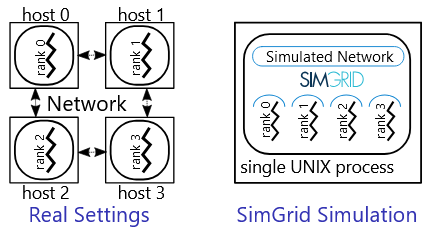
\includegraphics[scale=1.6]{SMPI.PNG}
	\caption{نمای کلی از نحوه کارکرد \lr{SimGrid} و \lr{SMPI} را در فرآیند شبیه‌سازی یک برنامه \lr{MPI}}\label{SMPI}
\end{figure}


\begin{itemize}
	\item نوشتن کد برنامه \lr{MPI}
	
	ابتدا باید یک برنامه ساده \lr{MPI} نوشته شود. این برنامه می‌تواند به زبان \lr{C} یا \lr{C++} نوشته شود و از توابع استاندارد \lr{MPI} برای ارتباط بین فرآیندها استفاده کند. به عنوان مثال، یک برنامه ساده که پیام‌های بین دو فرآیند را ارسال و دریافت می‌کند.
	
	\item کامپایل برنامه با  \lr{SMPI}
	
	پس از نوشتن برنامه، از کامپایلر \lr{smpicc} برای کامپایل کردن کد استفاده می‌شود. این کامپایلر همانند \lr{mpicc} عمل می‌کند اما برنامه را برای اجرای شبیه‌سازی در محیط \lr{SimGrid} آماده می‌کند.
	
\begin{figure*}
	\centering
	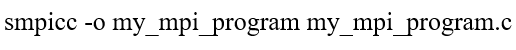
\includegraphics[scale=1]{Form3.PNG}
\end{figure*}
	
	\item ایجاد فایل پیکربندی 
	
	در صورت نیاز، می‌توان یک فایل پیکربندی برای تعیین پارامترهای شبیه‌سازی مانند تعداد فرآیندها، تعریف توپولوژی شبکه، مدل‌های مصرف انرژی، مدل‌های پردازشی، پیکربندی‌های شبیه‌سازی خاص و پارامترهای مرتبط با زمان‌بندی، ایجاد کرد.  برای تعریف توپولوژی شبکه می‌توان با استفاده از یک فایل \lr{XML}، لینک‌های ارتباطی و پهنای باند گره‌ها را مشخص کرد.

 همچنین با استفاده از \lr{SMPI} می‌توان مصرف انرژی فرآیندها را شبیه‌سازی کرد. این بخش از فایل پیکربندی می‌تواند شامل پارامترهایی برای تعیین میزان مصرف انرژی در هر گره و ارتباطات بین گره‌ها باشد. مدل‌های پردازشی مختلفی را برای شبیه‌سازی عملکرد پردازنده‌ها تعریف کرد. این مدل‌ها می‌توانند شامل زمان‌بندی فرآیندها، مدل‌های حافظه و غیره باشند. پیکربندی‌های خاص شامل تنظیمات خاصی مانند فعال یا غیرفعال کردن گزارش‌های خاص، تغییر سطح دقت شبیه‌سازی و یا تنظیم پارامترهای دقیق‌تری برای مدل‌های شبیه‌سازی است. پارامتر \lr{tracing:yes} به معنای فعال کردن قابلیت ردیابی و \lr{surf/precision:1e-9} به معنای تنظیم دقت شبیه‌سازی است. پارامترهای مرتبط با نوع زمان‌بندی فرآیندها و تخصیص منابع را مشخص کرد. این پارامترها تعیین می‌کنند که چگونه فرآیندها به منابع سیستم دسترسی دارند و چگونه منابع بین آن‌ها تقسیم می‌شود.
	\begin{figure*}
		\centering
		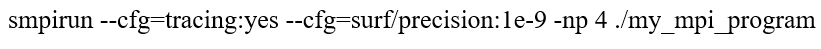
\includegraphics[scale=0.9]{Form1.PNG}
	\end{figure*}
	
	\item اجرای شبیه‌سازی با \lr{SMPI}
	
	برای اجرای برنامه، از دستور \lr{smpirun} استفاده می‌شود. این دستور تعداد فرآیندها و سایر پارامترهای شبیه‌سازی را مشخص می‌کند. پارامتر \lr{-np 2} تعداد فرآیندهایی که باید اجرا شوند را تعیین می‌کند.
	
	\item مشاهده و تحلیل نتایج
	
	پس از اجرای شبیه‌سازی، خروجی برنامه در ترمینال نمایش داده می‌شود. این خروجی می‌تواند شامل نتایج محاسبات، پیام‌های ارسال و دریافت شده، و زمان‌های اجرای فرآیندها باشد. این نتایج می‌توانند برای تحلیل عملکرد برنامه استفاده شوند.
	
\end{itemize}
\subsection{ابزار \lr{FBSPonMPI}}
در این رساله با کمک نرم‌افزار شبیه‌سازی \lr{SimGrid} ابزاری به نام \lr{FBSPonMPI} به‌منظور شبیه‌سازی پردازش مورد نظر طراحی شده است (شکل \ref{Tool} را ببینید). جزئیات بخش‌های آن‌ در ادامه به صورت مختصر شرح داده می‌شوند. 
\begin{figure*}[!h]
	\centering
	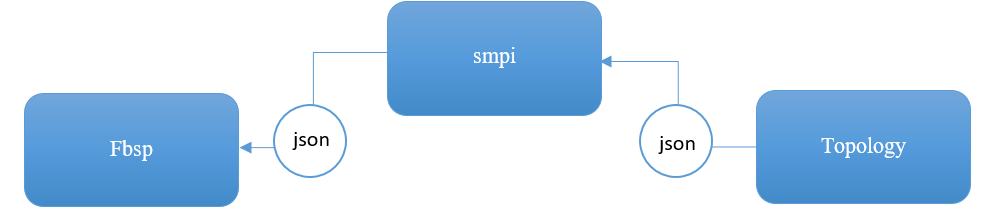
\includegraphics[width=16cm]{MyTool.png}
	\caption{شمای کلی ابزار \lr{FBSPonMPI}}
	\label{Tool}
\end{figure*}
\subsubsection{توپولوژی}
بخش اول ابزار از یک کد پایتون  با مجموعه کلاس‌های \lr{Data}، \lr{ICSCluster}، \lr{SimgridXML} و \lr{Topology}  تشکیل شده است. کلاس \lr{Topology} وظیفه ساخت توپولوژی شبکه بر اساس پارامترهای ورودی را دارد. ساخت این توپولوژی می‌تواند به‌صورت تصادفی یا بر اساس تنظیمات مورد نظر باشد. ماتریس مجاورت توپولوژی ایجادشده در این بخش در اختیار بخش‌های دیگر ابزار قرار می‌گیرد. کلاس \lr{SimgridXML} وظیفه ایجاد فایل پیکربندی \lr{simgrid} بر اساس توپولوژی ایجاد شده را بر عهده دارد.  این پیکربندی نحوه و نوع اتصال فرآیندها به یکدیگر در شبکه را مشخص می‌کند. این پیکربندی برای شبیه‌سازی عملکرد و رفتار برنامه‌های محاسبات توزیع‌شده با استفاده از \lr{SimGrid} مورداستفاده قرار می‌گیرد. 

در کلاس \lr{ICSCluster} منطقه‌بندی شبکه ایجاده شده در مرحله قبل با استفاده از روش خوشه‌بندی ساختار-محتوایی انجام خواهد شد. در این مورد، ساختار به معنای اتصالات و روابط گره‌ها و محتوا به معنای ویژگی‌های مرتبط با گره‌ها است. خروجی این کلاس یک فایل \lr{json} می‌باشد که شامل تعداد منطقه‌ها و اعضای آن است. این فایل نیز توسط بخش دوم ابزار مورداستفاده قرار می‌گیرد. کلاس \lr{Data} وظیفه تولید یا آماده‌سازی داده‌های اولیه برای پردازنده‌ها را بر عهده دارد و خروجی آن به صورت ‌یک فایل \lr{json} است که در اختیار هر پردازنده قرار خواهد گرفت. 

\subsubsection{\lr{SMPI}}
این بخش، هسته اصلی ابزار \lr{FBSPonMPI} است که توسط مولفه \lr{SMPI} از شبیه‌ساز \lr{SimGrid} توسعه‌ یافته است. این مولفه امکان شبیه‌سازی عملکرد برنامه‌های \lr{MPI} را فراهم می‌کند و به کاربران امکان می‌دهد بدون نیاز به سخت‌افزار واقعی، عملکرد برنامه‌های خود را در یک محیط شبیه‌سازی‌شده آزمایش کنند. شکل \ref{SMPI_ph} پردازش انجام‌شده در این بخش را نشان می دهد که از سه قسمت اصلی \lr{adapt}، \lr{communication}  و \lr{combine} تشکیل شده است.   داده، توپولوژی شبکه، اطلاعات مربوط به منطقه‌ها و فایل پیکربندی که در بخش قبل ایجاد شده‌اند در اختیار \lr{smpi} قرار می‌گیرند و پردازش توزیع‌شده به‌صورت شبیه‌سازی‌شده اجرا می‌شود و نتایج بدست آمده توسط هر پردازنده در یک فایل \lr{json} قرار می‌گیرند تا در انتهای فرآیند یادگیری توزیع‌شده تجمیع شده و برای رسم نمودارها مورد استفاده قرار گیرند.

\begin{figure*}[!h]
	\centering
	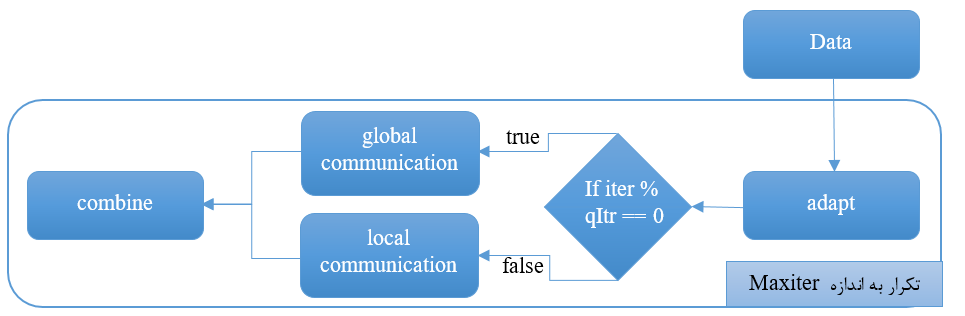
\includegraphics[width=16cm]{SMPI_Phases.png}
	\caption{مراحل پردازش در بخش \lr{SMPI}}
	\label{SMPI_ph}
\end{figure*}

در بخش \lr{FBSP} ابزار، تمامی داده‌های تولیدشده توسط \lr{smpi} برای تحلیل و رسم نمودار مورد استفاده قرار می‌گیرند.



\section{پیاده‌سازی محیط غیرایستا در آزمایشات}
یک الگوریتم یادگیری تطبیقی باید در هر محیطی توانایی یادگیری بالایی داشته باشد. در برخی از محیط‌ها مدل سیستم در طول زمان ثابت است و دست‌خوش تغییرات نمی‌شود. در این حالت با یک محیط ایستا\footnote{\lr{Stationary}} روبه‌رو هستیم. در حالتی که مدل سیستم ثابت نباشد و در طول زمان تغییر کند، یک محیط غیرایستا\footnote{\lr{non-Stationary}} خواهیم داشت. در اکثر موارد، کارایی و عملکرد یادگیری الگوریتم‌های تطبیقی انتشاری در محیط‌های غیرایستا با مشکل مواجه خواهد شد. به منظور بررسی توانایی ردیابی الگوریتم‌های یادگیری پیشنهادی، در آزمایشات از مدل ردیابی \ref{Track} استفاده شده است.
\begin{equation}
	Tracking\quad model:
	\begin{cases} 
		w_{o,t}=w_o+\omega_t\\
		\omega_t=0.9\omega_{t-1}+q_t
	\end{cases}
	\label{Track}
\end{equation}
که $q_t$ مجموعه‌ای از آشفتگی‌های \footnote{\lr{Perturbations}} مستقل با توزیع یکسان \footnote{\lr{Independent and Identically Distributed (iid)}} هستند که دارای میانگین صفر و ماتریس کوواریانس $Q$ می‌باشد و این مجموعه در هر تکرار مستقل از رگرسیون‌های ورودی و نویز خروجی است. پارامتر $Q$ به صورت $\sigma_q^2 I$ تعریف می‌شود و مقدار $\sigma_q^2$ برابر $10^{-4}$ است. در آزمایشات، عملکرد الگوریتم‌های یادگیری پیشنهادی در محیط غیرایستا در شرایطی کاملا یکسان و همانند محیط ایستا مورد بررسی قرار می‌گیرند. 
\section{نویزهای گاوسی و غیر گاوسی استفاده شده در آزمایشات}
وجود نویزهای مختلف در محیط پیاده‌سازی شبکه غیرقابل اجتناب است. نویزهای می‌توانند گاوسی یا غیرگاوسی باشند. ‌‌نویز گاوسی یک نویز استاتیکی است که از تابع توزیع چگالی احتمال نرمال یا همان تابع گاوسی پیروی می‌کند و مقادیر این نویز، توزیع گاوسی دارند. نویز غیرگاوسی از الگوی متقارن و زنگی شکل توزیع گاوسی منحرف می‌شود و از منابع نویز غیرتعادلی ناشی می‌شود. نویزهای غیرگاوسی حاکی از رخدادهای شدید در دامنه هستند که در نویز گاوسی وجود ندارند و رفتارشان به شدت تغییر می‌کند. در اغلب مطالعات به دلیل سادگی تشخیص و امکان دستیابی به برخی نتایج تحلیلی هنگام کار با نویزهای گاوسی، منبع نویز گاوسی در نظر گرفته می‌شود. عمدتاً به دلیل مشکلاتی که در کار با نویزهای غیرگاوسی وجود دارد، استفاده از آن‌ها به ندرت اتفاق می‌افتد. در این رساله، نویزهای غیر گاوسی با توزیع آلفا پایدار\footnote{\lr{$\alpha$-stable distribution}} و گاوسی آمیخته\footnote{\lr{Mixture Gaussian}} مدل‌سازی شده‌اند.

همان‌طور که ذکر شد، یکی از نویزهای غیرگاوسی که نویز پایدار $\alpha$ یا $\alpha-stable$ نامیده می‌شود از طریق توزیع $V_{\alpha-stable}(\alpha_{\nu},\beta_\nu,\gamma_{\nu},\delta_\nu)$ \cite{alphastable} مدل شده است و تابع مشخصه آن توسط رابطه \ref{alpha} تعریف می‌گردد:
\begin{equation}\label{alpha}
	\log \phi(t)=
	\begin{cases}
		-\gamma_{\nu}^{\alpha_{\nu}}|t|^\alpha_\nu\{1-i\beta_\nu sign(t)\tan\frac{\pi\alpha_\nu}{2}\}+i\delta_\nu t,\qquad\alpha_\nu\ne1\\
		-\gamma_\nu|t|\{1+i\beta_\nu sign(t)\frac{2}{\pi}\log|t|\}+i\delta_\nu t   \quad\qquad \alpha_\nu=1,
	\end{cases}
\end{equation}
که $\alpha_{\nu}$ پارامتر توانی است که در بازه $]0,2)$ قرار دارد. پارامتر مکانی $\delta_\nu\in \mathbb{R}$ توزیع را به سمت چپ یا راست شیفت می‌دهد. پارامتر مقیاس $\gamma_{\nu}>0$ توزیع را در حدود $\delta_\nu$ فشرده یا گسترش می‌دهد و پارامتر تقارن $\beta_\nu\in \left(-1,1\right]$ چولگی \footnote{\lr{Skewed}} توزیع را تعیین می‌کند. هنگامی که $\beta_\nu$ مثبت است، توزیع به سمت راست منحرف می شود و هنگامی که منفی است توزیع به سمت چپ منحرف می‌شود. زمانی‌که $\beta_\nu=0$، توزیع متقارن است \cite{alphastable_1999} و \cite{alphastable}.

همچنین، نویز گاوسی آمیخته به صورت زیر مدل شده است:
\begin{equation}
	(1-\theta)\mathcal{N}(\mu_1,\sigma_1^2)+\theta\mathcal{N}(\mu_2,\sigma_2^2)
\end{equation}
به منظور تولید نویز تکانشی\footnote{\lr{Impulsive noise}} یا داده‌های پرت بزرگ، باید پارامتر $\theta$ با یک مقدار کوچک تنظیم شود و $\sigma_1^2<<\sigma_2^2$ باشد. پارامتر مدل نویز برداری به صورت $V_{mix}(\mu_1,\mu_2,\sigma_1^2,\sigma_2^2,\theta)$ تعریف می‌شود. 
\section{توابع خطا بررسی‌شده در آزمایشات}
تابع خطا نقش بسزایی در کارایی و همگرایی الگوریتم‌های یادگیری انتشار دارد. در نتیجه انتخاب یک تابع خطای متناسب با مساله کاربردی و نوع نویزهای محیطی بسیار مهم و قابل توجه است. در طراحی تابع هزینه استفاده شده در فرایند یادگیری الگوریتم \lr{DSGD} معمولی از مربع خطا با فرم میانگین (امیدریاضی) $E\{l(e)\}=E\{e^2\}$ استفاده شده است. 

به منظور مقاوم‌سازی الگوریتم \lr{DSGD} در برابر انواع نویزهای محیطی در طراحی تابع هزینه آن انواع توابع خطا از جمله  \lr{pseudo-Huber loss}، \lr{Geman-McClure loss}، \lr{welsch loss} و \lr{cauchy loss} را مورد بررسی قرار داده‌ایم. تابع خطا  شبه‌هابر یا \lr{pseudo-Huber loss} تقریب نرمی از خطا هابر است که پیوسته و مشتق‌پذیر می‌باشد. تابع هزینه در الگوریتم پیشنهادی \lr{Robust Diffusion SGD} (\lr{RِDSGD}) بر اساس تابع خطا شبه‌هابر طراحی شده است که فرم میانگین آن به صورت زیر تعریف می‌شود:
\begin{equation}
	E\{l_\delta(e)\}=E\{\delta^2(\sqrt{1+(\frac{e}{\delta})^2}-1)\}
\end{equation}

که $\delta$ یک پارامتر اضافی برای کنترل شیب در زمان بروز خطاها با مقادیر بزرگ است. مزیت اصلی خطا شبه‌هابر این است که تابع آن دو بار مشتق‌پذیر بوده و نرم است؛ در حالی‌که خطا هابر غیرمحدب است و ممکن است الگوریتم‌های بهینه‌سازی در کمینه‌های محلی گیر کنند. 

شکل \ref{lossFun} منحنی رفتار برخی از توابع خطا از جمله تابع مربع خطا، خطا‌ شبه‌هابر، خطا \lr{welsch}، خطا \lr{Geman-McClure} و خطا \lr{cauchy} در مقابل مقادیر مختلف خطا نشان می‌دهد. در این شکل، پارامتر $\delta$ در خطا شبه‌هابر و پارامتر $c$ در خطا \lr{Geman-McClure} با مقدار $0.8$ تنظیم شده‌اند. همان‌طور که مشاهده می‌شود، تابع خطا شبه‌هابر مشتق‌پذیر است و نسبت به سایر توابع خطا نرم‌تر می‌باشد. همچنین نسبت به تابع مربع خطا حساسیت کمتری به داده‌های پرت و نویزها در داده‌های ورودی دارد.

\begin{figure}
	\centering
	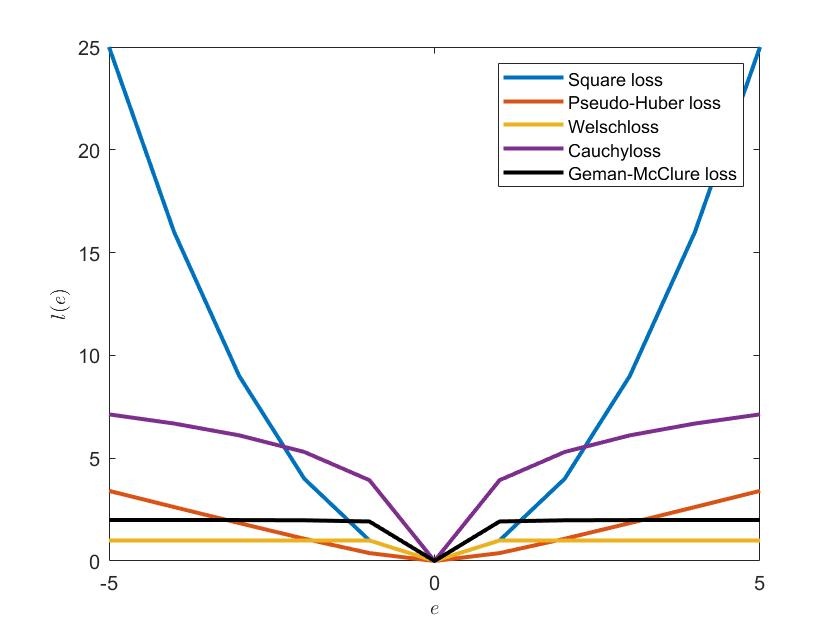
\includegraphics[scale=0.3]{CompareLoss.jpg}
	\caption{نمایش برخی از توابع خطا}\label{lossFun}
\end{figure}

\section{پیچیدگی محاسباتی الگوریتم یادگیری پیشنهادی}
در این بخش پیچیدگی محاسباتی الگوریتم یادگیری توزیع‌شده پیشنهادی بر اساس تعداد ضرب‌ها و جمع‌های استفاده شده در رابطه به‌روزرسانی گره $k$ در هر تکرار $t$ مورد بحث قرار می‌گیرد. پیچیدگی محاسباتی به صورت تابعی از پارامترهای $M$ (مرتبه فیلتر یا طول بردار پارامترها) و $N$ (تعداد گره‌ها در شبکه) بیان می‌شود. تعداد عملیات استفاده شده در الگوریتم \lr{RDSGD} به فرم \lr{ATC} در جدول \ref{tableexample} لیست شده‌اند. پیچیدگی محاسباتی \lr{RDSGD} از مرتبه $O(NM)$ است.


\begin{table}
	\centering
	\caption{هزینه محاسباتی الگوریتم \lr{RDSGD} برای گره $k$ در هر تکرار  }\label{Compexity}
	\begin{tabular}{ccc}\hline
		\lr{Term} & \lr{Multiplication Op.} & \lr{Addition Op.} \\\hline
		$\sum_{l\in N_k}a_{lk} w_{l,t-1}$ & $NM$ & $(N-1)M$  \\\hline
		$S_t^{-1}$ & $2M^2+2M$ & $3M^2-1$ \\\hline
		$\mu S_t^{-1}\lambda\left(\sum_{l\in N_k}a_{lk} w_{l,t-1}\right)$ & $M^2$ & $(M-1)M$  \\\hline
		$w^T_{k,t}u_{k,t}$ & $M$ & $M-1$  \\\hline
		$e_k(t)=d_k(t)-w_{k,t-1}^T u_{k,t}$ & 0 & 1  \\\hline
		$e_k(t)u_{k,t}$& $M$ & 0  \\\hline
		$\sqrt{1+\left(\frac{e_k(t)}{\delta}\right)^2}$ & 3 & 1  \\\hline
		$\frac{e_k(t)u_{k,t}}{\sqrt{1+\left(\frac{e_k(t)}{\delta}\right)^2}}$ & $M$ & 0  \\\hline
		$\sum_{l\in N_k}a_{lk}\frac{e_k(t)u_{k,t}}{\sqrt{1+\left(\frac{e_k(t)}{\delta}\right)^2}}$ & $NM$ & $(N-1)M$  \\\hline
		$\mu S_t^{-1}\sum_{l\in N_k}a_{lk}\frac{e_k(t)\textbf{u}_{k,t}}{\sqrt{1+\left(\frac{e_k(t)}{\delta}\right)^2}}$ & $M^2$ & $(M-1)M$ \\\hline
		$w_{k,t}$  & 0 & $2M$   \\\hline
		\textbf{\lr{Total}}  & $2NM+4M^2$ & $2NM+5M^2$  \\
		\textbf{\lr{per iteration}} & $+5M+3$ & $-M$ \\\hline
	\end{tabular}
	\label{tableexample}
\end{table}

تعداد عملیات ضرب و جمع الگوریتم یادگیری \lr{DSGD} به ترتیب $2NM-4M^2-4M$ و $2NM+5M^2-M-1$ است. در حالی‌که $N>M$ باشد، پیچیدگی محاسباتی الگوریتم یادگیری \lr{DSGD} از مرتبه $O(NM)$ است. الگوریتم‌های \lr{DSGD} و \lr{RDSGD} از لحاظ مرتبه زمانی مشابه هستند و اختلاف تعداد عملیات ضرب و جمع آن‌ها اندک است که با توجه به مقاوم بودن و کارایی بالا الگوریتم یادگیری \lr{RDSGD} این اختلاف قابل چشم‌پوشی است. از آنجایی‌که رابطه به‌روزرسانی الگوریتم \lr{DRLS} در گام تطبیق برای هر گره در هر تکرار $t$ شامل عملیات ماتریسی از اندازه $M\times M$ می‌باشد، پیچیدگی محاسباتی آن از مرتبه $O(NM^2)$ است. بنابراین پیچیدگی محاسباتی الگوریتم یادگیری \lr{RDSGD} با مرتبه $O(NM)$ خیلی کمتر از پیچیدگی محاسباتی الگوریتم \lr{DRLS} است. درحالی‌که رفتار همگرایی \lr{RDSGD} در برابر نویز گاوسی و در محیط ایستا تقریبا مشابه‌ رفتار همگرایی \lr{DRLS} است اما در حضور نویزهای غیرگاوسی  و به خصوص در محیط‌های غیرایستا، \lr{RDSGD} بر الگوریتم یادگیری \lr{DRLS} غلبه می‌کند. 
تعداد عملیات ضرب مورد نیاز در الگوریتم‌های \lr{DLMS} و \lr{RDLMS} به ترتیب $2NM+M$ و $2NM+4M+3$ است. همچنین تعداد عملیات جمع آن‌ها به ترتیب $2NM-M$ و $2NM+1$ می‌باشد. علی‌رغم وجود اختلاف در تعداد عملیات محاسباتی الگوریتم‌های \lr{DLMS}،  \lr{RDLMS} و \lr{RDSGD}، به دلیل مقاوم بودن و کارایی \lr{RDSGD} این اختلاف قابل چشم‌پوشی است. در جدول \ref{CompareCompexity} پیچیدگی محاسباتی این الگوریتم‌ها به طور مختصر با هم مقایسه شده‌اند. 
\begin{table}
	\centering
	\caption{مقایسه پیچیدگی محاسباتی برخی از الگوریتم‌های تطبیقی انتشاری}\label{CompareCompexity}
	\begin{tabular}{|c@{\hspace{6mm}}|@{\hspace{9mm}}c@{\hspace{19mm}}
			|}
		\hline
		\lr{Computational Complexity} & \lr{Algorithm}   \\
		\hline
		$O(NM+M)$ & \lr{DLMS} \\
		\hline  
		$O(NM+M)$ & \lr{RDLMS} \\
		\hline 
		$O(NM^2)$ & \lr{DRLS} \\
		\hline
		$O(NM+M^2)$ & \lr{DSGD} \\
		\hline
		$O(NM+M^2)$ & \lr{RDSGD} \\
		\hline      
	\end{tabular}
\end{table}



\section{الگوریتم‌های مورد مقایسه در آزمایشات}
در این بخش الگوریتم‌ها و روش‌های ارائه شده توسط محققان دیگر که مشابه روش پیشنهادی بوده و در بخش ارزیابی با آن مقایسه شده‌اند، ذکر می‌شوند.

\subsection{الگوریتم‌های مورد مقایسه از جنبه روش‌های مختلف یادگیری تطبیقی توزیع‌شده }
به منظور بررسی کارایی و رفتار همگرایی الگوریتم یادگیری پیشنهادی، الگوریتم‌های یادگیری انتشاری مشابه ارائه شده در سایر تحقیقات از جمله  \lr{DLMS}، \lr{DRLS}، \lr{DMCC}، \lr{DLMF}، \lr{DSignLMS} و \lr{Robust DLMS} مورد مقایسه قرار داده شده‌اند. الگوریتم‌های \lr{DRLS}  \cite{Cat20082} و \lr{DLMS}  \cite{Lop2008} به ترتیب نسخه‌های توزیع‌شده انتشاری الگوریتم‌های \lr{RLS} و \lr{LMS} می‌باشند. الگوریتم انتشار معيار حداكثرسازي کورآنتروپی (\lr{DMCC}) \cite{MA2016} مبتنی بر مفاهیم تئوری اطلاعات است و از كرنل گوسي به دليل توانايي آن در رد كردن نمونه‌هاي آغشته به نويز غيرگوسي جهت مقاوم‌سازی رویکرد یادگیری استفاده شده است.

در الگوريتم توزیع‌شده انتشاری  \lr{DLMF} \cite{Park2014} ميانگين توان چهارم خطا در تابع هدف براي مقابله با نويز غيرگوسي به كارگرفته شده است. همچنين در الگوريتم انتشار \lr{Robust DLMS} \cite{Ashk} از تابع زيان شبه‌هابر به منظور مقابله با نویزهای گاوسی و غیرگاوسی استفاده شده است. الگوريتم انتشار علامت خطا \lr{DSignLMS} \cite{Ni2016}  یک الگوریتم یادگیری مبتني بر حداقل‌سازي ميانگين مربعات خطا است که از علامت خطا در تابع هدف استفاده می‌کند. 


\subsection{الگوریتم‌های مورد مقایسه از جنبه روش‌های مختلف همگام‌سازی}
به منظور ارزیابی رویکرد پیشنهادی از دیدگاه عملی علاوه‌بر استفاده از معیارهای کارایی آماری و سخت‌افزاری بر روی مجموعه داده‌های مصنوعی و واقعی، مقایسه آن با سایر رویکردهای پیشین از جمله  \lr{PSP}، \lr{Sync-Switch } و \lr{RNA Protocol } انجام می‌شود. 

همگام‌سازی در رویکرد \lr{PSP} \cite{Zhao2021} به روش احتمالی کنترل می‌شود، یعنی با نمونه‌برداری از گره‌های شرکت‌کننده در یادگیری درصدی از گره‌های سیستم که مرحله فعلی را به پایان رسانده‌اند را تخمین می‌زند. ایده اصلی روش \lr{PSP} این است که ما نیاز داریم فقط بخشی از گره‌ها نه همه آنها، در پروسه همگام‌سازی قرار بگیرند.  

روش  \lr{Sync-Switch} \cite{Syncswitch2021} مبتنی بر یک روش همگام‌سازی ترکیبی است و با بهره‌گیری از مزایای \lr{BSP} و \lr{ASP} با کاهش زمان یادگیری به طور هم‌زمان دقت همگرایی را حفظ می‌کند. فرایند یادگیری با مکانیزم همگام‌سازی \lr{BSP} آغاز می‌شود و در صورت برقراری یکی از شرایط 1) رسیدن به یک دقت همگرایی مشخص یا 2) به‌وجود آمدن کند‌کننده‌های گذرا،  مکانیزم همگام‌سازی به \lr{ASP} تغییر می‌کند. 

در روش \lr{RNA Protocol }   \cite{Mitigating2020} به منظور مقابله با مساله کندکننده‌ها در یادگیری توزیع‌شده از الگوریتم غیرمتمرکز \lr{AllReduce} جزئی برای مدیریت کلاسترهای ناهمگن بهره گرفته شده است. در این پروتکل، یک گره آغازگر به صورت تصادفی از بین گره‌ها انتخاب می‌شود. زمانیکه کار گره آغازگر کارش تمام شود، صرف نظر از اینکه سایر گره‌ها محاسبات‌شان را تمام کرده باشند یا خیر، عمل کاهش در کل شبکه انجام خواهد شد.

\section{نتایج آزمایش‌ها}
در این بخش نتایج بدست آمده از آزمایشات انجام شده بر روی داده‌های مصنوعی (داده‌های تولید شده به صورت تصادفی) و داده‌های واقعی، ارائه خواهد شد. ارزیابی و مقایسه‌ها در این فصل به دو بخش اصلی تقسیم می‌شود. بخش اول مربوط به ارزیابی الگوریتم‌های یادگیری تطبیقی انتشاری پیشنهادی می‌باشد و پس از آن در بخش دوم به ارزیابی رویکرد پیشنهادی پرداخته می‌شود.

\subsection{ارزیابی الگوریتم \lr{DSGD} در مساله شناسایی سیستم}
با انجام مجموعه‌ای از آزمایشات، کارایی و رفتار همگرایی الگوریتم یادگیری انتشاری \lr{DSGD} (الگوریتم \ref{Alg_DSGD}) را مورد ارزیابی و مقایسه با الگوریتم‌های یادگیری انتشاری دیگر قرار می‌دهیم. بدین منظور کلیه الگوریتم‌های یادگیری انتشاری به فرم \lr{ATC} در نظر گرفته شده‌اند و در این بخش آزمایشات بر روی  شبکه‌ای با 20 گره که توپولوژی آن در ابتدای هر شبیه‌سازی به طور تصادفی تولید می‌شود، انجام شده‌اند.

\begin{figure}
	\centering
	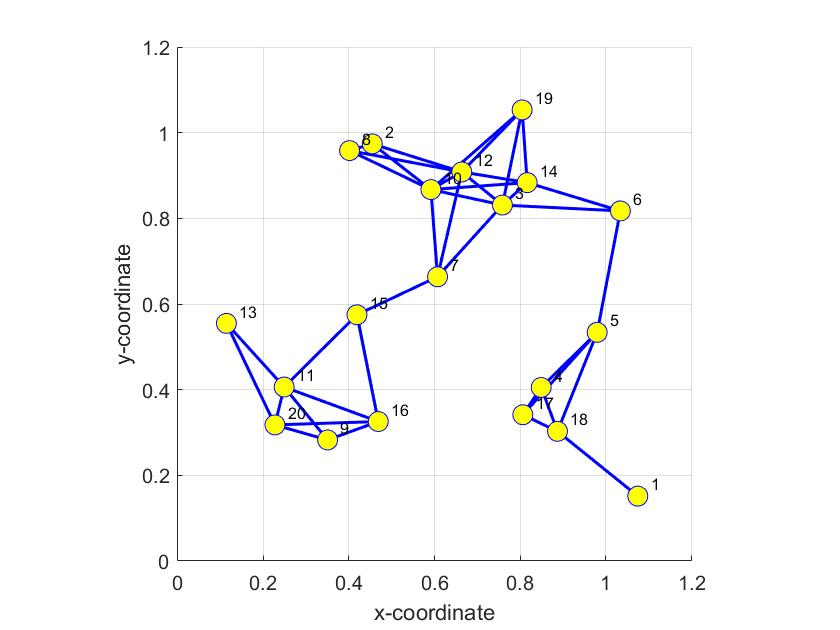
\includegraphics[scale=0.4]{topotogy.jpg}
	\caption{نمونه‌ای از توپولوژی شبکه تصادفی تولید شده با 20 گره}\label{Topology}
\end{figure}

پروفایل آماری شبکه در شکل \ref{Power} نشان می‌دهد که قدرت سیگنال و نویز گره‌ها در یک شبکه متفاوت است. الگوریتم \lr{DSGD} در \lr{MATLAB} پیاده‌سازی شده است و  عملکرد الگوریتم‌ها بر حسب میانگین انحراف مربع (\lr{MSD}) شبکه بر روی مساله شناسایی سیستم اندازه‌گیری شده است که به صورت زیر تعریف می‌شود:
\begin{equation}\label{MSD}
	MSD^{network}(t)=\frac{1}{N}\sum_{k=1}^{N}E||w_o-w_{k,t}||^2
\end{equation}
مساله شناسایی سیستم در واقع علم ساخت مدل‌های ریاضی سیستم‌ها از روی داده‌های ورودی-خروجی است که در دهه‌های گذشته \cite{Sam2013} توجه زیادی را به خود جلب کرده است. شمای کلی یک گره در یک شبکه تطبیقی توزیع‌شده برای کاربرد شناسایی سیستم در شکل \ref{p13} در فصل \ref{ProposedApproach} نشان داده شده است. 
\begin{figure}
	\centering
	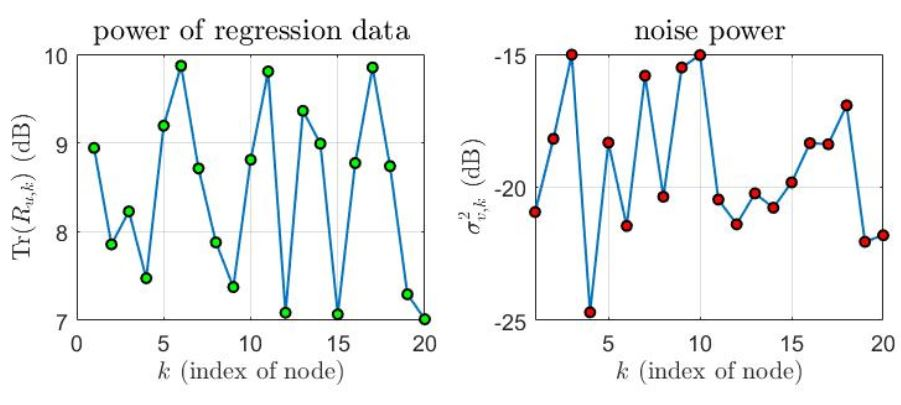
\includegraphics[scale=0.8]{regressor_noise_power__.jpg}
	\caption{واریانس‌های نویز و ردیابی کوواریانس‌های رگرسیون برای 20 گره}\label{Power}
\end{figure}

 در آزمایشات انجام شده اندازه گام (پارامتر نرخ یادگیری) به طور پیش‌فرض برای تمام الگوریتم‌ها $\mu=0.03$ تنظیم شده است؛ اگر برای الگوریتمی مقداری غیر از این باشد، حتما ذکر خواهد شد. همان‌طور که قبلا اشاره شد، ماتریس $S_t$ تاثیر قابل توجهی در تسریع نرخ همگرایی الگوریتم دارد. به منظور بررسی تاثیر آن بر نرخ همگرایی، دو حالت ثابت و متغیر را برای ماتریس $S_t$ در نظر می‌گیریم. در اولین حالت ماتریس $S_t=S$ را با ماتریس همانی از سایز $M\times M$ مقداردهی و نسخه ثابتی از الگوریتم $DiffusionSGD$ به نام $DSGD$ معرفی می‌شود. در حالت دیگر، ماتریس $S_t$ با هر نمونه داده ورودی جدید با زمان تغییر می‌کند. نسخه متغیر الگوریتم $DiffusionSGD$ به نام $DRSGD$ معرفی می‌شود. شکل \ref{Com_DSGD_DRSGD} منحنی‌های یادگیری سه الگوریتم، $SGD$ ساده بدون هیچ استراتژی انتشار و دو نسخه ثابت و متغیر الگوریتم $DiffusionSGD$ را بر اساس معیار $MSD$ مورد مقایسه قرار می‌دهد. در این آزمایش پارامترهای $\mu=0.03$, $M=5$, $T=500$ است و نتایج از میانگین 20 اجرای مستقل حاصل شده‌اند. 
 
 نتایج شبیه‌سازی تأثیر استراتژی‌انتشار و مقدار ماتریس $S_t$ را بر نرخ همگرایی نشان می‌دهد و به وضوح بیان می‌کند که روش \lr{DRSGD} سریع‌تر از دو روش دیگر همگرا می‌شود. در اجرای روش \lr{DRSGD}، از ایده محاسبه $R^{-1}$ در الگوریتم \lr{RLS} برای تنظیم $S_t$ در هر تکرار $t$ استفاده کردیم. این روش از توانایی بیشتری در استخراج اطلاعات مفید از سیگنال‌های نویزدار برخوردار است.
 
 \begin{figure}
 	\centering
 	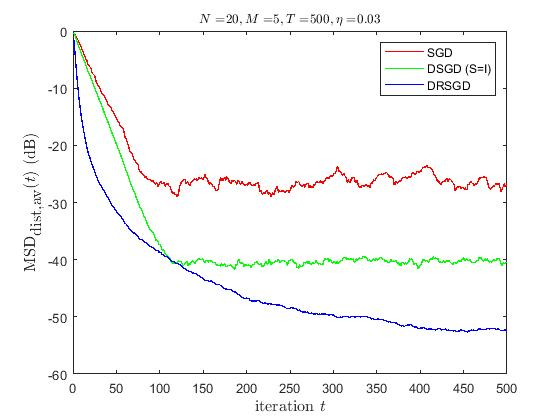
\includegraphics[scale=0.6]{Compare_DSGDandDRSGD_Gaussiannoise_F.jpg}
 	\caption{مقایسه الگوریتم‌های \lr{SGD} و \lr{DSGD} و \lr{ِDRSGD} با 500 تکرار و $M=5$ }\label{Com_DSGD_DRSGD}
 \end{figure}


یکی دیگر از پارامترهای موثر بر عملکرد و نرخ همگرایی الگوریتم\lr{DSGD} اندازه گام $\mu_t=\mu$ است. شکل \ref{DifferentMu} نتایج اعمال شش مقدار متفاوت $\mu$ را در الگوریتم \lr{DSGD} نشان می‌دهد. بر اساس نتایج ارائه شده، برای تضمین همگرایی سریع‌تر، مقدار $\mu$ نباید خیلی کوچک باشد و بهترین همگرایی زمان رخ می‌دهد که مقدار $\mu=0.03$ تنظیم شود.

\begin{figure}
	\centering
	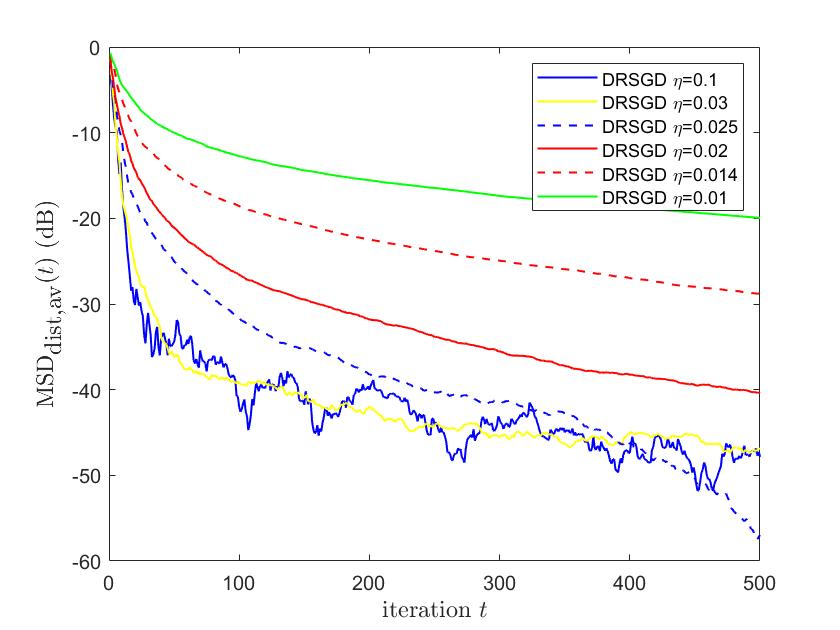
\includegraphics[width=5in]{Dif_eta.jpg}
	\caption{\lr{MSD} شبکه گذرا الگوریتم \lr{DSGD} با مقادیر  متفاوت اندازه گام در 500 تکرار و $M=5$}\label{DifferentMu}
\end{figure}

در آزمایش بعدی، از سنجه جدید اختلاف همگرایی وزنی \ref{DeltaW} برای بررسی همگرایی الگوریتم \lr{DSGD} استفاده شده است. شکل \ref{Delta_w} رفتار الگوریتم را بر اساس معیار اختلاف همگرایی وزنی $\Delta(w_{k,t},w_{k,t-1},w)$ در تکرارهای مختلف نشان می‌دهد. همان‌طور که دیده می‌شود، معیار $\Delta(w_{k,t},w_{k,t-1},w)$ در طول زمان روند کاهشی دارد و این بدین معناست که بردار تخمین‌زده شده در تکرار $t$ ،$w_t$، به بردار وزن دلخواه $w$ نزدیکتر از بردار تخمین‌زده شده در تکرار قبلی $w_{t-1}$ است.

\begin{figure}
	\centering
	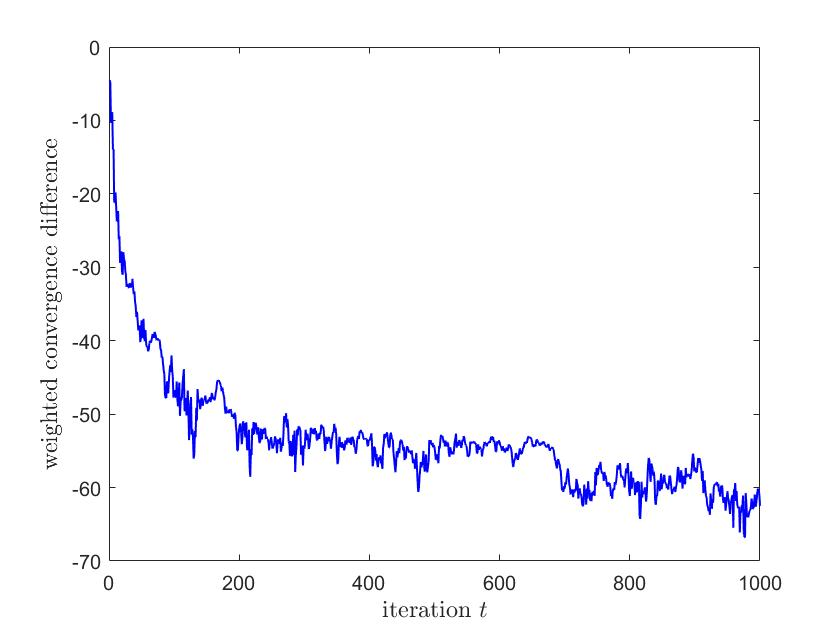
\includegraphics[scale=0.4]{deltaW_1000Sample_new.jpg}
	\caption{منحنی کارایی الگوریتم پیشنهادی بر اساس معیار اختلاف همگرایی وزنی در 1000 تکرار اول با طول بردار وزن 5}\label{Delta_w}
\end{figure}

در آزمایش بعدی، تأثیر توپولوژی شبکه بر عملکرد روش \lr{DSGD} بر اساس معیار اختلاف همگرایی وزنی، $\Delta(w_{k,t},w_{k,t-1},w)$ بررسی شده است. ما روش \lr{DSGD} را روی چهار توپولوژی مختلف شبکه با 20 گره اعمال کرده و منحنی‌های عملکرد آن را در 100 تکرار اول نشان داده‌ایم. چهار توپولوژی‌ مختلف از یک شبکه با 20 گره را می‌توان در شکل \ref{fourTop} مشاهده کرد. بر اساس نتایج نشان داده شده در شکل \ref{DifferentTop}، می‌توان نتیجه گرفت که معیار $\Delta(w_{k,t},w_{k,t-1},w)$ در طول فرایند یادگیری الگوریتم \lr{DSGD} در تمام توپولوژی‌های شبکه روند کاهشی دارد. این موضوع نشان می‌دهد که بردار وزن $w_t$ در طول زمان به بردار وزن بهینه $w$ نزدیکتر می‌شود.

\begin{figure}
	\centering
	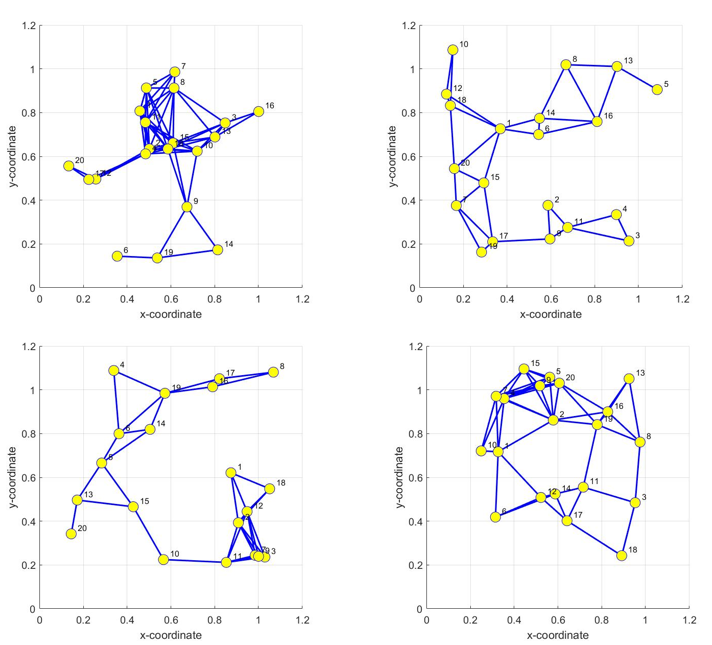
\includegraphics[scale=1]{Four_Topo.PNG}
	\caption{توپولوژی‌های مختلف شبکه}\label{fourTop}
\end{figure}


\begin{figure}
	\centering
	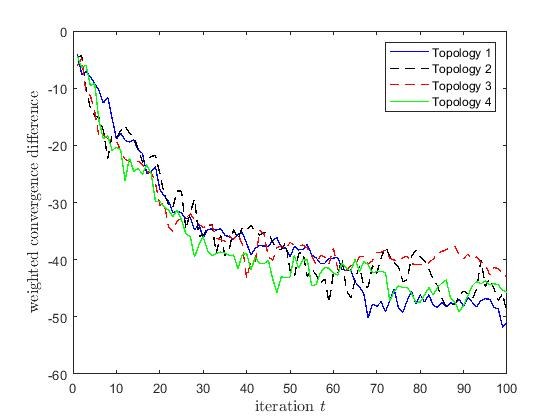
\includegraphics[scale=0.55]{Dif_Topo.jpg}
	\caption{منحنی عملکرد الگوریتم پیشنهادی بر روی شبکه هایی با توپولوژی متفاوت }\label{DifferentTop}
\end{figure}

عملکرد و سرعت همگرایی الگوریتم پیشنهادی در حالت متغیر \lr{DRSGD} را با الگوریتم‌های \lr{DLMS} معمولی، \lr{DRLS} معمولی، الگوریتم‌های \lr{DMCC} و \lr{ِDLMF} در فرم \lr{ATC} مقایسه کرده‌ایم. در این آزمایش، فرایند یادگیری با 500 و 1000 تکرار مورد بررسی قرار گرفته است. به منظور داشتن نرخ همگرایی اولیه یکسان در تمام الگوریتم‌های مورد مقایسه، اندازه گام $\mu=0.03$ در نظر گرفته شده است. شکل \ref{Com_DRSGD_LMS_RLS} منحنی مقادیر \lr{MSD} برای الگوریتم‌های مورد مقایسه در محیطی آغشته به نویز گاوسی با 500 تکرار فرایند یادگیری را نشان می‌دهد. 

همانطور که مشاهده می‌شود، نرخ همگرایی الگوریتم پیشنهادی \lr{DRSGD} سریع‌تر از الگوریتم‌های \lr{DLMS}، \lr{DMCC} و \lr{DLMF} می‌باشد، در حالی‌که نرخ همگرایی \lr{DRSGD} کمی کمتر از \lr{DRLS} است. با افزایش تعداد تکرارها از 500 به 1000 تکرار در شکل \ref{n700}، مشاهده می‌شود که\lr{DRSGD} به منحنی \lr{MSD} بهتری دست می‌یابد و تقریبا همانند الگوریتم \lr{DRLS} رفتار می‌کند. این اختلاف ناچیز در مقایر همگرا شده را می‌توان در مقابل اختلاف بین پیچیدگی محاسباتی \lr{DRSGD} و \lr{DRLS} نادیده گرفت. پیچیدگی محاسباتی الگوریتم‌های انتشار بر حسب تعداد عملیات ضرب و جمع در هر تکرار برای هر گره برحسب پارامترهای $M$ (طول بردار وزن یا اندازه فیلتر) و $N$ (تعداد کل گره‌های شبکه) مورد بحث قرار می‌گیرد. از آنجایی که \lr{DRLS} شامل عملیات ماتریسی با اندازه $M*M$ در مرحله انطباق در هر تکرار $t$ برای هر گره است، پیچیدگی محاسباتی آن از مرتبه $O(NM^2)$ است، که در آن $N$ عدد است. همانطور که انتظار می‌رود، از آنجایی که $N>M$، پیچیدگی محاسباتی الگوریتم پیشنهادی \lr{DRSGD}، با مرتبه $O(NM)$، بسیار کمتر از \lr{DRLS} است. علاوه‌بر این، \lr{DRLS} فقط برای یادگیری آنلاین مناسب است، در حالی‌که \lr{DRSGD} برای یادگیری آنلاین و آفلاین کاربرد دارد. از سوی دیگر، \lr{DRLS} به ترتیب ورود داده‌ها حساس است اما \lr{DRSGD} به این مورد حساس نیست.

\begin{figure}
	\centering
	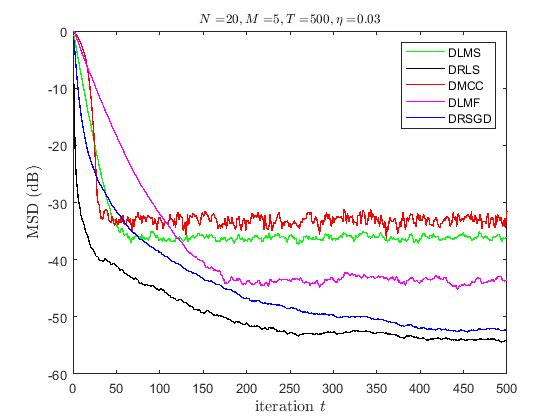
\includegraphics[scale=0.5]{Compare5Algorithm.jpg}
	\caption{مقایسه بین الگوریتم پیشنهادی و الگوریتم‌های انتشار بر روی \lr{MSD} با 500 تکرار و طول فیلتر 5}\label{Com_DRSGD_LMS_RLS}
\end{figure}


\begin{figure}
	\centering
	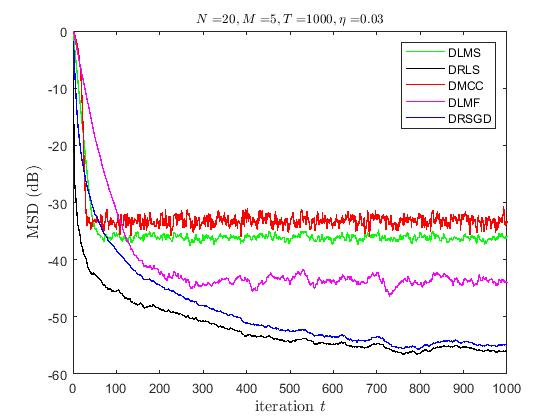
\includegraphics[scale=0.5]{1000.jpg}
	\caption{مقایسه بین الگوریتم پیشنهادی و الگوریتم‌های انتشار بر روی \lr{MSD} با 1000 تکرار و طول فیلتر 5}\label{n700}
\end{figure}

\subsection{ارزیابی الگوریتم \lr{RDSGD} در محیط ایستا}
استفاده از توابع زیان مقاوم در برابر نویزهای مختلف محیطی سبب افزایش مقاومت روش الگوریتم یادگیری توزیع‌شده می‌شود. تابع زیان مربع خطا  تنها در برابر نویزهای گاوسی مقاوم است اما در محیط‌های آغشته به نویزهای غیرگاوسی عملکرد ضعیفی دارد و در اکثر مواقع واگرا می‌شود. توابع زیانی مانند شبه‌هابر، کورآنتروپی و ... نسبت به نویزهای غیرگاوسی مقاوم می‌باشند. 

در این بخش، نتایج آزمایش‌ها برای نشان دادن عملکرد الگوریتم مقاوم \lr{RDSGD} در حل مسائل شناسایی سیستم و پیش‌بینی و همچنین بررسی تأثیر پارامترهای مختلف بر عملکرد تخمین آن ارائه می‌شوند. الگوریتم \lr{RDSGD} با الگوریتم‌های انتشار مرسوم و الگوریتم‌های انتشار قوی از نظر مقاوم بودن در محیط‌های ایستا و غیرایستا مورد مقایسه قرار خواهد گرفت. این مقایسه‌ها در حضور نویزهای گاوسی و غیر گاوسی ارزیابی می‌شوند. در این رساله، نویزهای غیر گاوسی با توزیع آلفا پایدار و گاوسی مخلوط مدل‌سازی می‌شوند. نویز آلفا پایدار به صورت $V_{\alpha-stable}(1.3, 0, 1.2, 0)$ تنظیم شده است. این مجموعه از آزمایش‌ها نیز بر روی شبکه‌ای با 20 گره و طول بردار وزن $M=5$ انجام شده‌اند. نتایج گزارش‌شده به صورت میانگین 20 آزمایش مستقل می‌باشند که عملکرد الگوریتم‌ها را برحسب معیار \lr{MSD} شبکه اندازه‌گیری می‌کنند.


برای ارزیابی عملکرد، رفتار یادگیری الگوریتم \lr{RDSGD} از نظر مقاوم بودن در برابر نویز برای مساله شناسایی سیستم با سایر الگوریتم‌ها مانند \lr{DMCC} \cite{MA2016}، \lr{DLMS} \cite{Lop2008}، \lr{DRLS} \cite{Cat20082}،\lr{DSGD}، \lr{DLMF} \cite{DLMF2017}، \lr{DsignLMS} \cite{DsignLMS2016} و \lr{RDLMS} مقایسه می‌شود. در این بخش، این مقایسه‌ها در محیطی ایستا و تحت نویز گاوسی و نویزهای غیرگاوسی مورد ارزیابی قرار می‌گیرند. یک محیط ایستا به مدل استاتیک سیستم در زمان اشاره می‌کند. اندازه گام $\mu$ برای \lr{DLMF} $0.25$، برای \lr{DLMS}، \lr{DRLS}، \lr{DSGD}، \lr{RDSGD} $0.03$، برای \lr{DMCC} $0.05$، برای \lr{DsignLMS} $0.09$  و برای \lr{RDLMS} $0.07$ تنظیم شده است. 
در آزمایش اول، منحنی عملکرد الگوریتم‌ها در محیط آغشته به نویز آلفا پایدار در شکل \ref{StAlpha} نشان داده شده‌اند.
\begin{figure}[htbp]  \centering{
		\subfigure[]{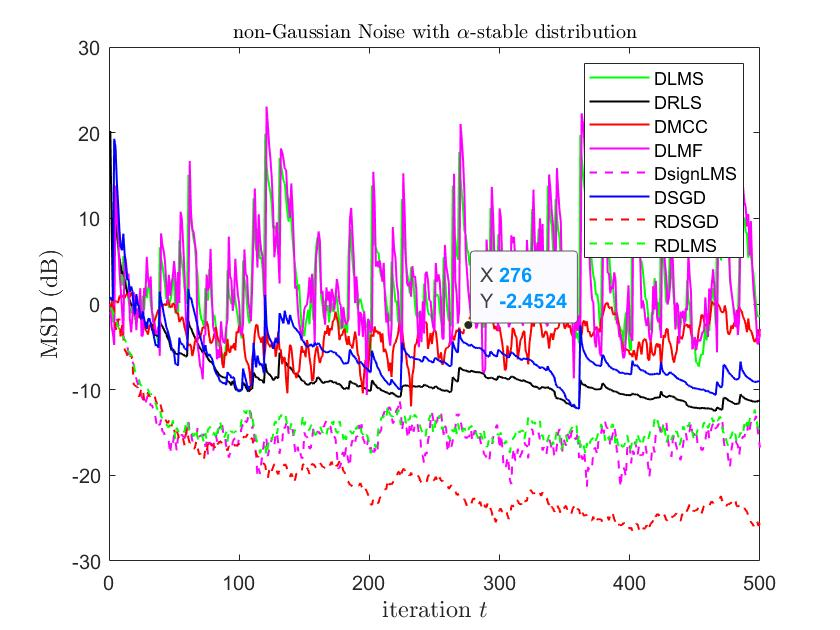
\includegraphics[width=10 cm,height=7 cm]{AllCom_AlphaSt8.png}\label{StAlpha}}
		\subfigure[]{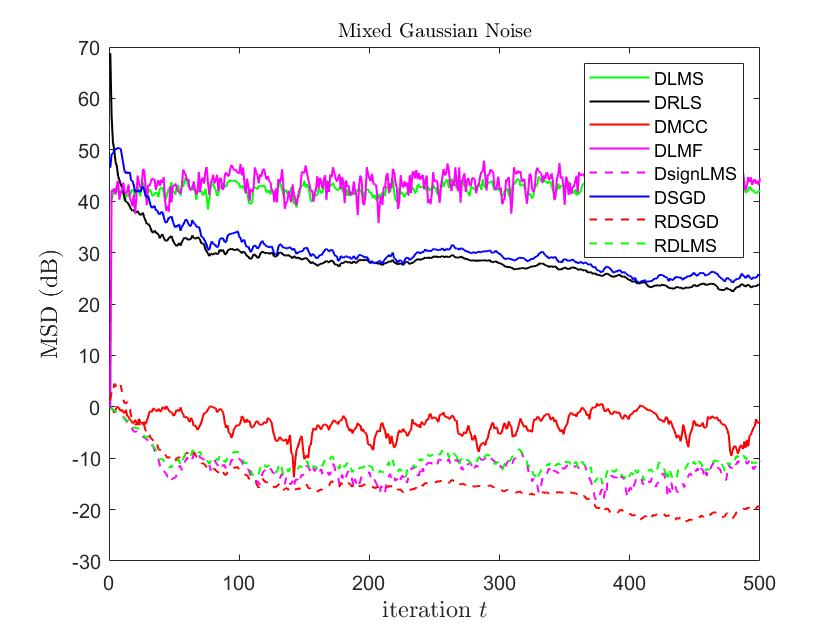
\includegraphics[width=10 cm,height=7 cm]{AllCom_MixGau_St8.png}\label{StMixGassian}}
		\\
		\subfigure[]{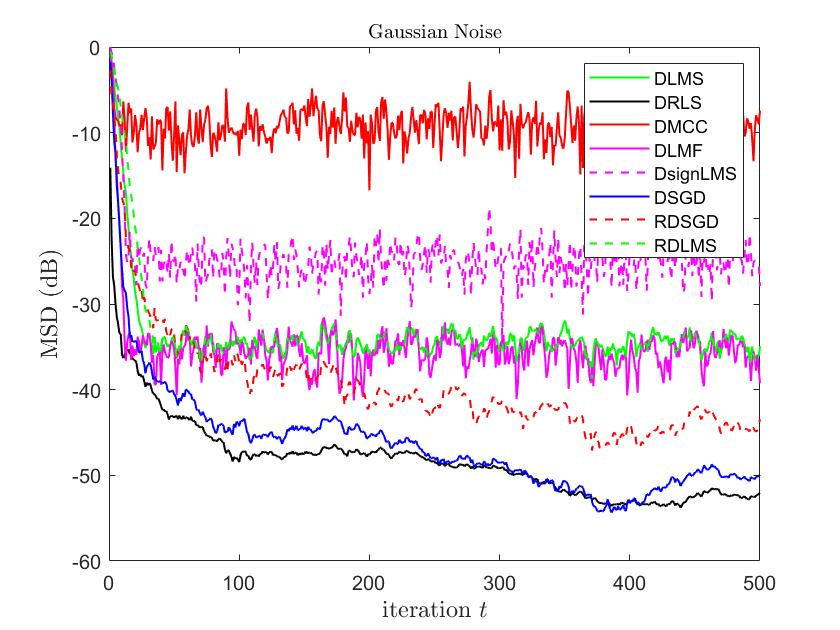
\includegraphics[width=10 cm,height=7 cm]{AllCom_Gau_St8.png}\label{StGaussian}}
	}
	\caption[]{مقایسه رفتار همگرایی الگوریتم‌ها در محیط ایستا. الف) نویز الفا پایدار با $SNR=-20 dB$
	ب) نویز گاوسی مخلوط با $SNR=-50 dB$
ج) نویز گاوسی با $SNR=20 dB$} 
	\label{AllStationary}
\end{figure}
همانطور که مشاهده می‌شود، \lr{DLMS}، \lr{DRLS}، \lr{DLMF}، \lr{DMCC} و \lr{DSGD} در حضور نویز پایدار $\alpha$ واگرا هستند و \lr{RDSGD}، \lr{RDLMS} و \lr{DisignLMS} نسبت به سایر الگوریتم‌ها در حالت پایدار با خطای کمتری همگرا می‌شوند. با این حال \lr{RDSGD} از سایر الگوریتم‌ها بهتر عمل می‌کند. نتایج ارائه شده در شکل \ref{StAlpha} نشان می‌دهند که الگوریتم پیشنهادی در برابر نویز پایدار $\alpha$ مقاوم است و سریع‌تر از سایر الگوریتم‌ها همگرا می‌شود.

شکل \ref{StMixGassian} منحنی رفتاری الگوریتم‌ها را بر حسب معیار \lr{MSD} در حضور نویز گاوسی مخلوط با $SNR=-50dB$ نشان می‌دهد. این نویز توسط  $GMM(\mu_{G1},\mu_{G2},\sigma)$ مدل‌سازی شده است. اندازه گام برای \lr{DMCC} $0.3$، برای \lr{DsignLMS} $0.09$، برای \lr{DLMF} $0.25$، برای \lr{RDLMS} $0.07$، برای \lr{DLMS}، \lr{DRLS}، \lr{DSGD} و \lr{RDSGD} $0.05$ تنظیم شده است. همانطور که در شکل \ref{StMixGassian}، برای نویز گاوسی مخلوط با $SNR=-50 dB$ و توزیع $GMM(\mu_{G1}=1,\mu_{G2}=300،\sigma=1)$ مشاهده می‌شود،  الگوریتم‌های \lr{DLMS} و \lr{DLMF} واگرا شده‌اند. \lr{RDSGD}، \lr{RDLMS}، \lr{DsignLMS} و \lr{DMCC} از الگوریتم‌های دیگر بهتر عمل می‌کنند در حالی‌که در حالت پایدار، \lr{RDSGD} بهتر از \lr{RDLMS}، \lr{DsignLMS} و \lr{DMCC} است و سریعتر به مقدار خطای کمتری همگرا می‌شود. بر این اساس، می‌توان نتیجه گرفت که \lr{RDSGD} از همه الگوریتم‌های رقیب مقاوم‌تر است و بهتر عمل می‌کند.

الگوریتم‌های انتشار مقاوم بسیاری پیشنهاد شده‌اند، اما عملکرد آنها برای مقابله با نویزهای گاوسی خوب نیست. اندازه گام $\mu$ برای \lr{DLMF} $0.15$، برای \lr{DLMF}، $0.05$ برای \lr{DLMS}، \lr{DRLS}، \lr{DSGD}، \lr{RDSGD}، $0.2$ برای \lr{DMCC}، $ 0.03$ برای \lr{DsignLMS} و $ 0.07$ برای \lr{RDLMS} تنظیم شده است. شکل \ref{StGaussian} نشان می‌دهد که \lr{DMCC} و \lr{DsignLMS} که برای نویزهای غیر گاوسی قوی هستند، اما در برابر نویز گاوسی خوب عمل نمی‌کنند. همانطور که مشاهده می‌شود، \lr{DRLS}، \lr{RDSGD} و \lr{DSGD} از \lr{DLMF}، \lr{DLMS} و \lr{RDLMS} بهتر عمل می‌کنند. \lr{DRLS} و \lr{DSGD} رفتار همگرایی تقریبا مشابهی دارند. با این حال، می‌توان نتیجه گرفت که الگوریتم پیشنهادی می‌تواند نویزهای گاوسی و غیر گاوسی را در محیط ایستا مدیریت کند.

اندازه گام $\mu$ پارامتر بسیار موثری بر کارایی و نرخ همگرایی الگوریتم \lr{RDSGD} است. در شکل \ref{mu_alpha} منحنی‌های کارایی \lr{RDSGD} به ازای مقادیر مختلف $\mu$ نشان داده شده است. از نتایج ارائه شده می‌توان نتیجه گرفت که مقدار $\mu$ نباید خیلی بزرگ یا خیلی کوچک باشد تا عملکرد و همگرایی سریع الگوریتم تضمین شود. بر اساس نتایج ارائه شده در شکل \ref{mu_alpha}، برای مساله شناسایی سیستم و در حضور نویز آلفا پایدار، مقدار مناسب $\mu$ برای \lr{RDSGD} $0.05$ است.

\begin{figure}[ht]
	\centering
	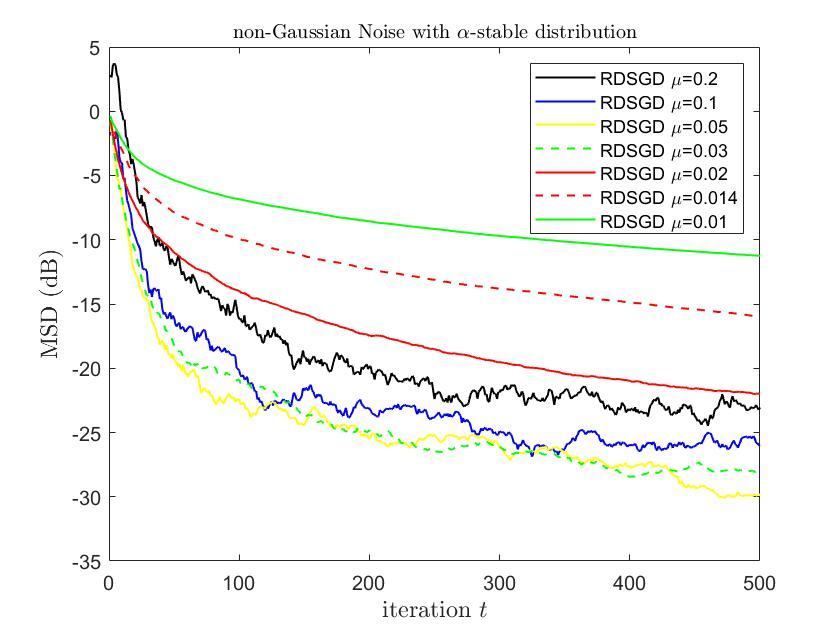
\includegraphics[scale=0.3]{mu_alpha_5Iter.jpg} 
	\caption{منحنی \lr{MSD} الگوریتم \lr{RDSGD} به ازای مقادیر مختلف اندازه گام در حضور نویز آلفا پایدار با $SNR=-20 dB$}
	\label{mu_alpha}
\end{figure}

شکل \ref{SSP_Sta} عملکرد گره‌های شبکه را در حالت پایدار با کمک منحنی \lr{MSD} در حضور نویزهای گاوسی، گاوسی آمیخته و نویز الفا پایدار در محیط ایستا نشان می‌دهد. همان طور که دیده می‌شود، گره‌ها در حالت پایدار به مقادیر خطای تقریبا نزدیک بهم همگرا می‌شوند. شکل \ref{SSP_1} نیز عملکرد گره‌های شبکه در حالت پایدار برای تعدادی از الگوریتم‌ها را مورد مقایسه قرار می‌دهد. 

\begin{figure}[ht]
	\centering
	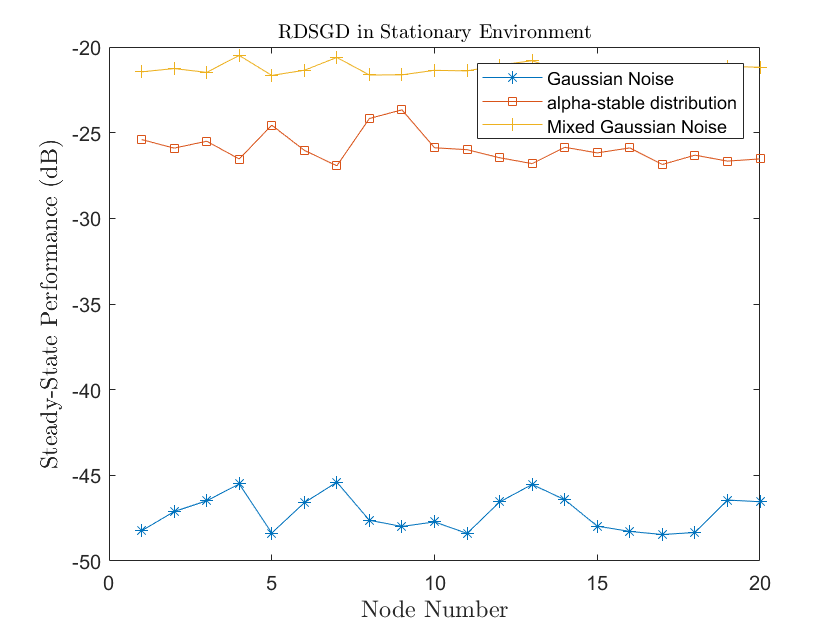
\includegraphics[scale=0.4]{SSP_Noise_Stationary_1.png} 
	\caption{منحنی \lr{MSD} عملکرد گره‌های مختلف در یک شبکه  با 20 گره در حالت پایدار}
	\label{SSP_Sta}
\end{figure}

\begin{figure}[htbp]  \centering{
		\subfigure[]{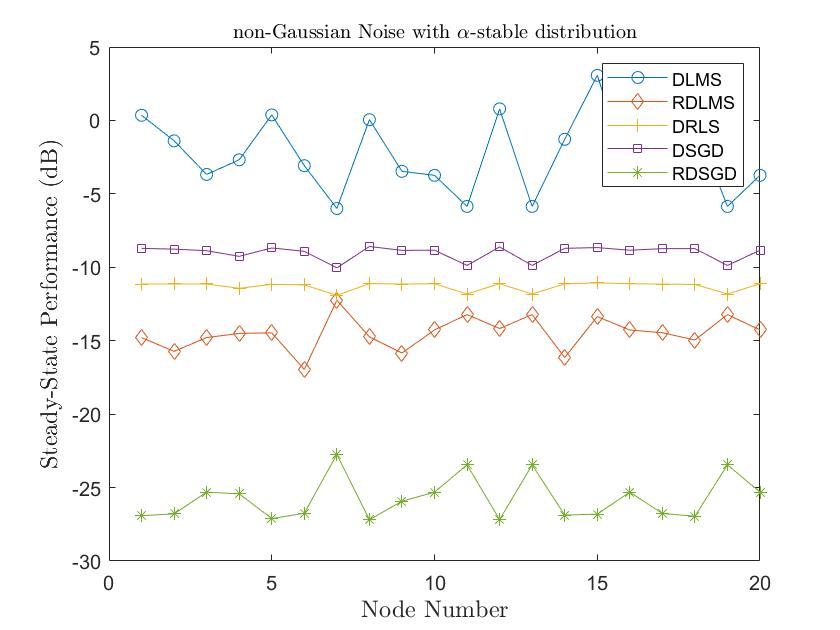
\includegraphics[width=10 cm,height=7 cm]{AlphaStable_SSP_.jpg}\label{SSP-alpha_}}
		\subfigure[]{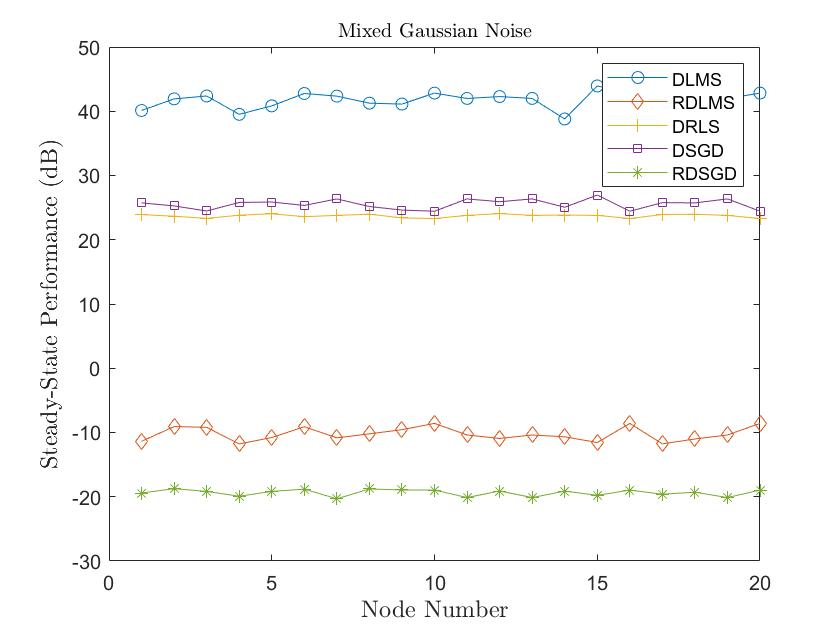
\includegraphics[width=10 cm,height=7 cm]{MixGaussian_SSP_.jpg}\label{SSP-mix_}}
		\\
		\subfigure[]{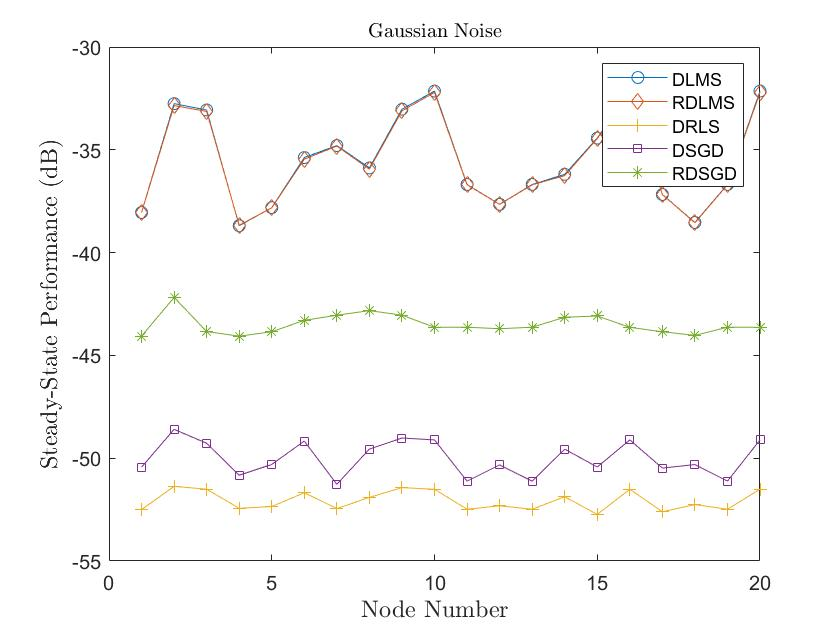
\includegraphics[width=10 cm,height=7 cm]{Gaussian_SSP_.jpg}\label{SSP-gaussian_}}
	}
	\caption[]{مقایسه رفتار همگرایی  گره‌ها در حالت پایدار  برای تعدادی از الگوریتم‌ها در محیط ایستا. الف) نویز الفا پایدار با $SNR=-30 dB$
		ب) نویز گاوسی مخلوط با $SNR=-50 dB$
		ج) نویز گاوسی با $SNR=20 dB$} 
	\label{SSP_1}
\end{figure}





\subsection{ارزیابی الگوریتم \lr{RDSGD} در محیط‌ غیرایستا}
محیط غیرایستا به حالتی اشاره دارد که  مدل سیستم در طول زمان تغییر می‌کند. آموزش الگوریتم‌های انتشار با عملکرد خوب در محیط‌های غیرایستا دشوار است و بسیاری از این الگوریتم‌ها توانایی ارائه نتایج قابل قبولی در محیط‌های غیرایستا ندارند. در ادامه، عملکرد \lr{RDSGD} در محیط غیرایستا مدل‌شده با \ref{Track} و در شرایطی مشابه با آزمایشات محیط ایستا بررسی می‌شود.

شکل \ref{non_1} رفتار همگرایی الگوریتم‌ها را در مقابل نویزهای گاوسی، گاوسی مخلوط و نویز الفا پایدار در محیط غیرایستا نشان می‌دهد. در حضور نویزهای غیرگاوسی، الگوریتم پیشنهادی قادر است تاثیر نمونه‌های اغشته به نویز را کاهش دهد. به عبارت دیگر، حساسیت کمتری به نویز دارد. همان‌طور که در شکل \ref{non-alpha} و \ref{non-mix} دیده می‌شود، الگوریتم \lr{RDSGD} در محیط غیرایستا به سایر الگوریتم‌های رقیب غلبه می‌کند. شکل \ref{non-gaussian} نشان می‌دهد که در حضور نویز گاوسی نیز الگوریتم پیشنهادی بر الگوریتم‌های \lr{DLMS}، \lr{DRLS}، \lr{DMCC}، \lr{DLMF}، \lr{DsignLMS} غلبه می‌کند و این در حالی است که الگوریتم \lr{DSGD} در حالت پایدار بهتر از \lr{RDSGD} عمل می‌کند و به سایر الگوریتم‌ها هم غلبه کرده است. 

\begin{figure}[htbp]  \centering{
		\subfigure[]{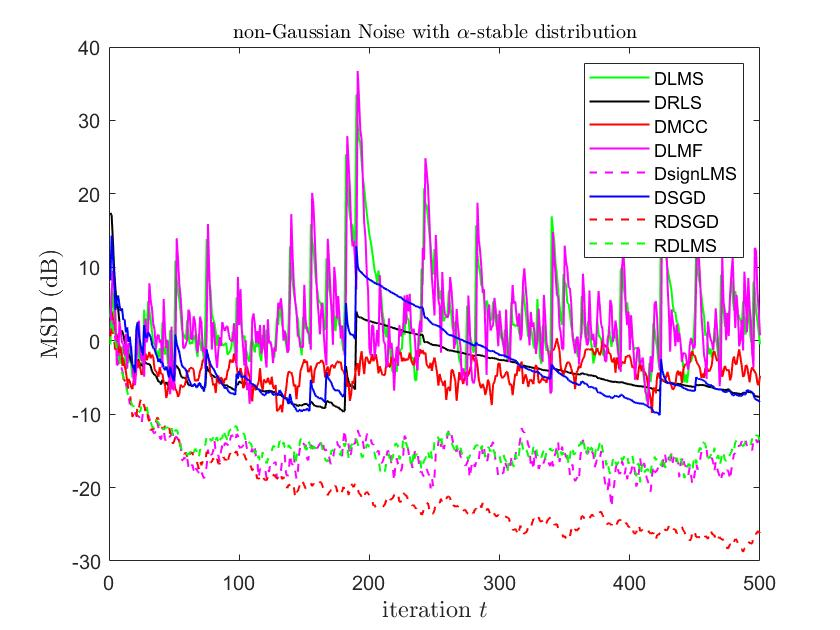
\includegraphics[width=10 cm,height=7 cm]{AllCom_AlphaNon8.png}\label{non-alpha}}
		\subfigure[]{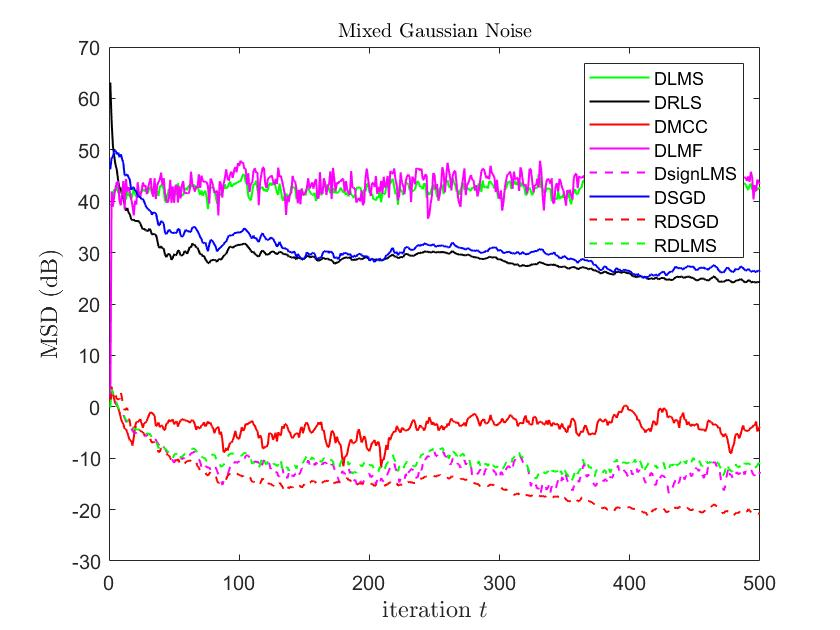
\includegraphics[width=10 cm,height=7 cm]{AllCom_MixGau_Non8.png}\label{non-mix}}
		\\
		\subfigure[]{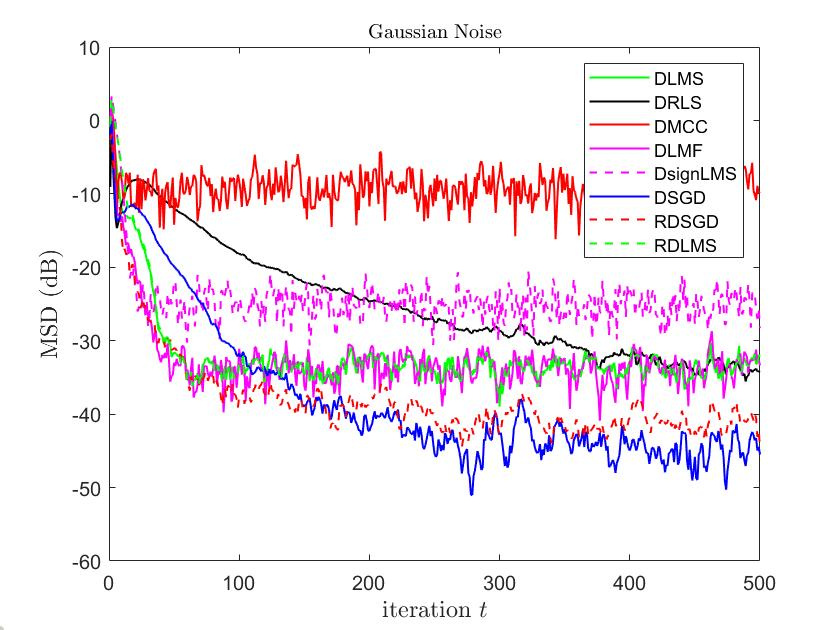
\includegraphics[width=10 cm,height=7 cm]{AllCom_Gau_Non8.png}\label{non-gaussian}}
	}
	\caption[]{مقایسه رفتار همگرایی الگوریتم‌ها در محیط غیرایستا. الف) نویز الفا پایدار با $SNR=-30 dB$
		ب) نویز گاوسی مخلوط با $SNR=-50 dB$
		ج) نویز گاوسی با $SNR=20 dB$} 
	\label{non_1}
\end{figure}

در آزمایشی دیگر، تاثیر توابع زیان مختلف بر رفتار همگرایی و میزان خطا در حالت پایدار الگوریتم \lr{DSGD} در محیط غیرایستا مورد بررسی و مطالعه قرار گرفته است. توابع زیان استفاده شده در این آزمایش شامل مربع خطا، شبه‌هابر، تابع زیان \lr{Cauchy} \cite{CauchyLoss}، \lr{Geman-McClure} \cite{GemanLoss}، \lr{Welsch} \cite{WelschLoss} می‌باشند که الگوریتم‌های متناظر با این توابع زیان به ترتیب \lr{DSGD}، \lr{RDSGD}، \lr{GemanDSGD}، \lr{CauchyDSGD} و \lr{WelschDSGD} نام‌گذاری شده‌اند. شکل \ref{OtherLoss} رفتار همگرایی این الگوریتم‌ها را در مقابل نویزهای گاوسی، گاوسی مخلوط و نویز الفا پایدار نشان می‌دهد. همان‌طور که در شکل \ref{OtherLossAlpha} دیده می‌شود، \lr{RDSGD} تا تکرار 600 به تمام الگوریتم‌ها غلبه کرده است، اما از آن به بعد \lr{RDSGD} و \lr{CauchyDSGD} تقریبا مشابه رفتار می‌کنند. 

همان‌طور که در شکل \ref{OtherLossMixGaussian} نشان داده است، در محیط آغشته به نویز گاوسی مخلوط، الگوریتم پیشنهادی  \lr{RDSGD} از همه الگوریتم‌ها بهتر عمل می‌کند و سریع‌تر از سایر الگوریتم‌ها به خطای کمتر در حالت پایدار همگرا می‌شود. شکل \ref{OtherLossGaussian} نشان می‌دهد که همه الگوریتم‌ها در برابر نویز گاوسی در محیط غیرایستا تقریباً یکسان عمل می‌کنند. با توجه به رفتار همگرایی الگوریتم‌ها در برابر سه نویز مورد بررسی، تابع زیان شبه‌هابر در مقایسه با سایر توابع زیان انتخاب مناسب‌تری است.

\begin{figure}[htbp]  \centering{
		\subfigure[]{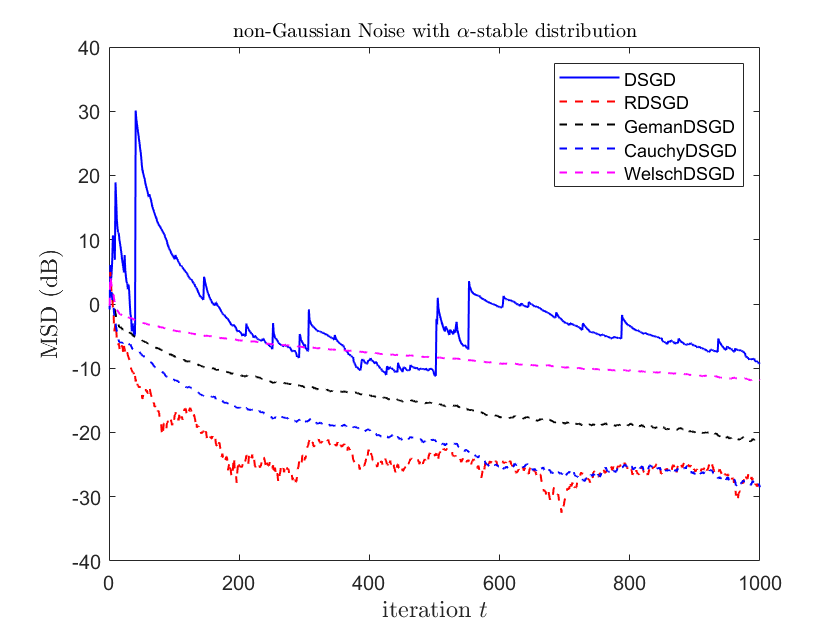
\includegraphics[width=9 cm,height=7 cm]{ComLossAlpha_non8.png}\label{OtherLossAlpha}}
		\subfigure[]{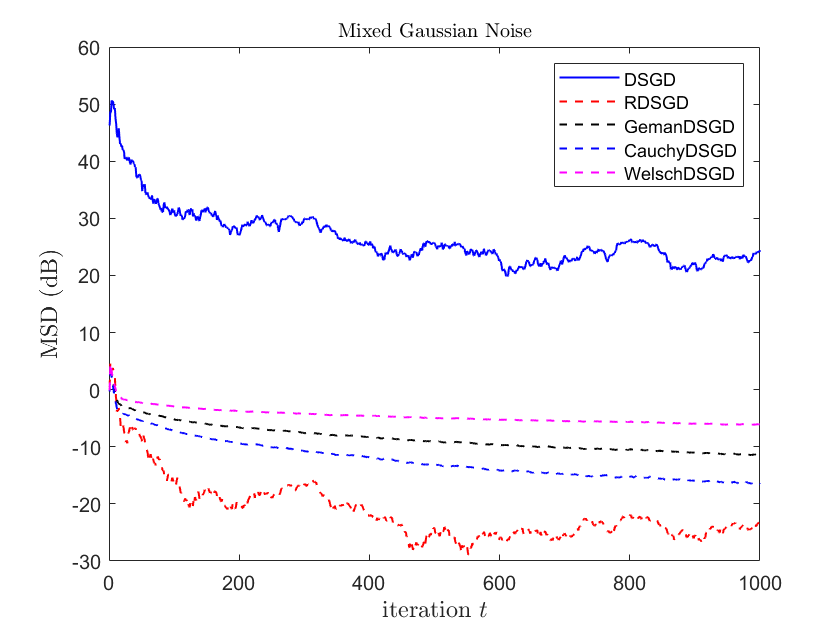
\includegraphics[width=9 cm,height=7 cm]{ComLossMixGau_non8.png}\label{OtherLossMixGaussian}}
		\\
		\subfigure[]{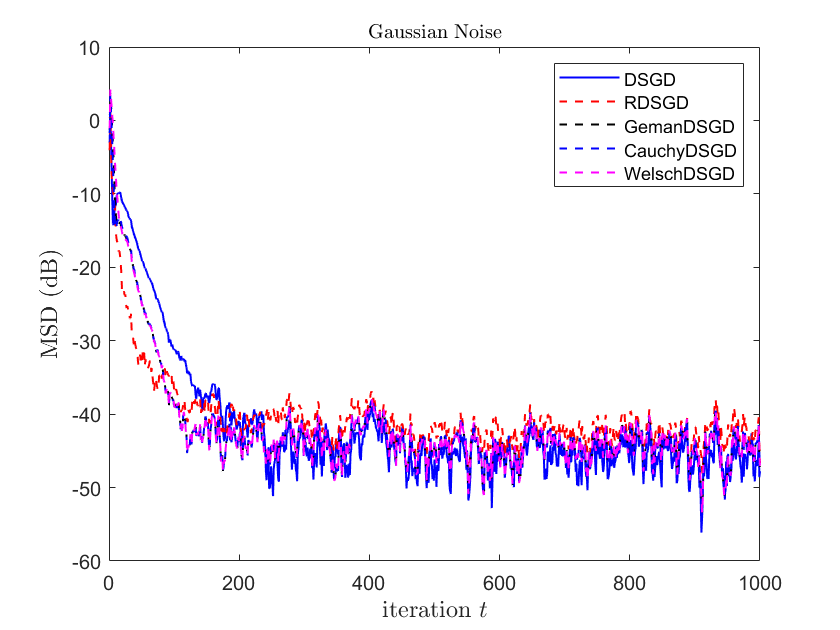
\includegraphics[width=9 cm,height=7 cm]{ComLossGau_non8.png}\label{OtherLossGaussian}}
	}
	\caption[]{تأثیر توابع زیان مختلف بر رفتار همگرایی الگوریتم \lr{DSGD} در محیط غیرایستا. الف) نویز الفا پایدار
		ب) نویز گاوسی مخلوط
		ج) نویز گاوسی} 
	\label{OtherLoss}
\end{figure}

شکل \ref{SSP_nonSta} عملکرد گره‌های شبکه را در حالت پایدار با کمک منحنی \lr{MSD} در حضور نویزهای گاوسی، گاوسی آمیخته و نویز الفا پایدار در یک محیط غیرایستا نشان می‌دهد. همان طور که دیده می‌شود، تمام 20 گره شرکت‌کننده در فرآیند یادگیری توزیع‌شده همگرا در حالت پایدار به مقادیر خطای تقریبا نزدیک بهم می‌شوند. شکل \ref{SSP_non_1} نیز عملکرد گره‌های شبکه در حالت پایدار برای تعدادی از الگوریتم‌ها را مورد مقایسه قرار می‌دهد. 

\begin{figure}[ht]
	\centering
	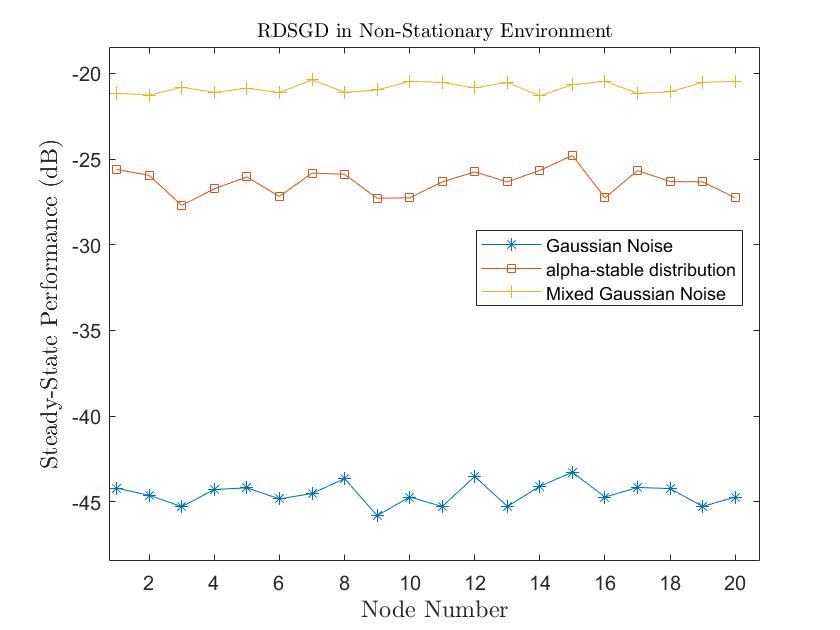
\includegraphics[scale=0.3]{SSP_Noise_non-Stationary.png} 
	\caption{منحنی \lr{MSD} عملکرد گره‌های مختلف در یک شبکه  با 20 گره در حالت پایدار}
	\label{SSP_nonSta}
\end{figure}

\begin{figure}[htbp]  \centering{
		\subfigure[]{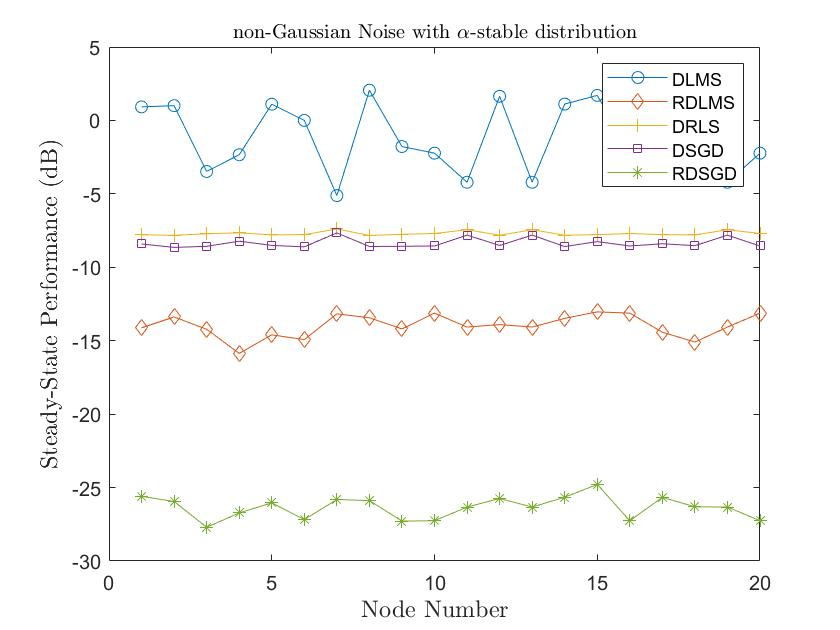
\includegraphics[width=10 cm,height=7 cm]{AlphaStable_SSP.jpg}\label{SSP-alpha}}
		\subfigure[]{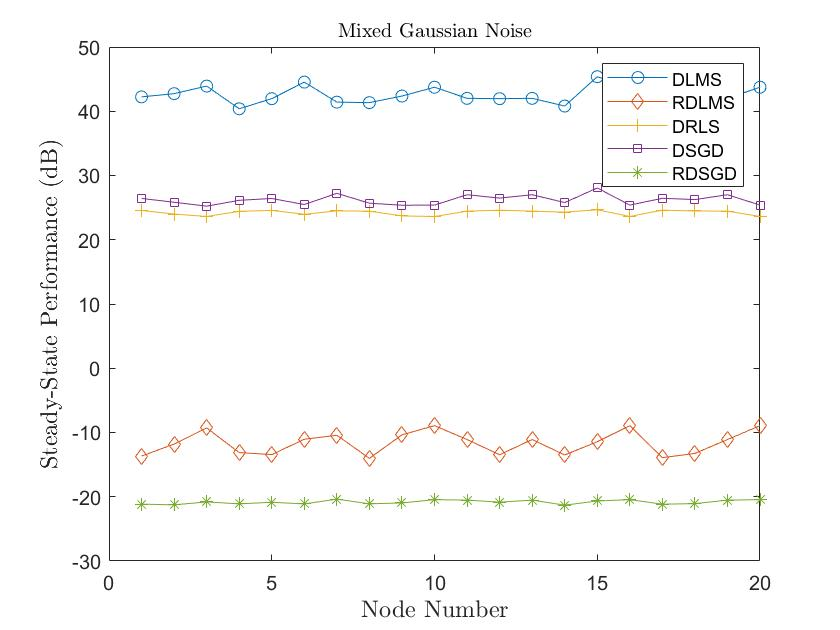
\includegraphics[width=10 cm,height=7 cm]{MixGaussian_SSP.jpg}\label{SSP-mix}}
		\\
		\subfigure[]{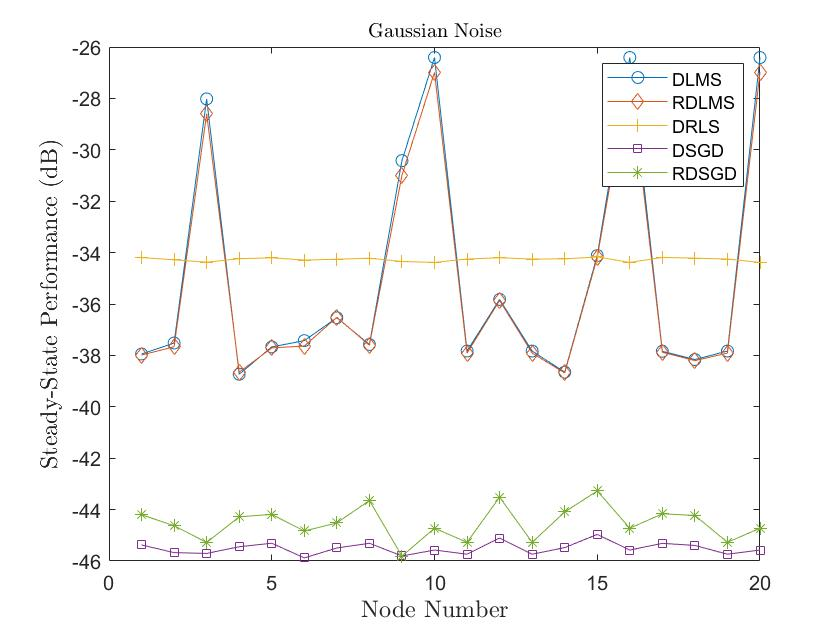
\includegraphics[width=10 cm,height=7 cm]{Gaussian_SSP.jpg}\label{SSP-gaussian}}
	}
	\caption[]{مقایسه رفتار همگرایی  گره‌ها در حالت پایدار  برای تعدادی از الگوریتم‌ها در محیط غیرایستا. الف) نویز الفا پایدار با $SNR=-30 dB$
		ب) نویز گاوسی مخلوط با $SNR=-50 dB$
		ج) نویز گاوسی با $SNR=20 dB$} 
	\label{SSP_non_1}
\end{figure}

\subsection{ارزیابی رویکرد یادگیری توزیع‌شده \lr{FBSP} در مساله شناسایی سیستم}
‌‌‌در این بخش نتایج آزمایشات انجام شده و تحلیل نتایج و مقایسه رویکرد پیشنهادی با دیگر روش‌ها مورد بررسی قرار می‌گیرد. کارایی رویکرد پیشنهادی را در محیطی شبیه‌سازی شده با استفاده از شبیه‌ساز \lr{SimGrid} بررسی می‌کنیم و آن را با روش‌های مشابه \lr{RNA}، \lr{Synch-Switch} و \lr{PSP} مقایسه می‌کنیم. در محیط شبیه‌سازی شده، گره‌ها با پردازنده‌ها و لینک‌هایی با پهنای باند متفاوت تعریف می‌شوند و تعداد یال‌های بین گره‌ها نشان‌دهنده فاصله آنها است که در شبیه‌سازی انجام شده از الگوریتم دیکسترا برای بدست آوردن کوتاه‌ترین مسیر بین هر جفت گره استفاده می‌شود. 

برای رسیدن به یک همگرایی مطلوب، برقراری تعادل بین دفعات اجرای ابرگام سراسری و ابرگام منطقه‌ای بسیار حائز اهمیت است. با هدف کاهش میزان ارتباطات بین گره‌ها و کاهش زمان انتظار آن‌ها، پارامتر کنترلی به نام $qIter$ معرفی شده است که مشخص‌کننده زمان اجرای ابرگام‌ سراسری در رویکرد پیشنهادی \lr{FBSP} است. شروع فرایند یادگیری با ابرگام سراسری بوده و بعد از اجرای $qIter-1$ بار ابرگام منطقه‌ای، یک بار ابرگام سراسری اجرا خواهد شد.

در آزمایش اول همگرایی رویکرد پیشنهادی \lr{FBSP} به ازای مقادیر متفاوت $1$، $10$، $50$ و $100$ برای پارامتر کنترلی $qIter$ بررسی شده است. زمانیکه پارامتر $qIter=1$ است، در واقع تمام ابرگام‌ها به صورت ابرگام سراسری اجرا می‌شوند. همانطور که قبلا هم اشاره شده است، توپولوژی شبکه به صورت یک گراف همبند پیاده‌سازی می‌شود و گره‌های شبکه بر اساس روش خوشه‌بندی ساختار-محتوایی منطقه‌بندی می‌شوند. گراف شبکه از لحاظ تعداد لینک‌ها و ارتباطات هر گره با سایر گره‌ها یا مجموعه همسایگی گره‌ها نباید خلوت باشد. این رویکرد یادگیری توزیع‌شده بر روی گراف‌های خلوت یا گراف‌هایی با تعداد لینک‌های کم به نتایج همگرایی مطلوبی دست پیدا نمی‌کند. شکل \ref{net100} یک شبکه با 100 گره و تعداد لینک‌های مناسب است که آزمایش مورد نظر بر روی این شبکه در یک محیط غیرایستا و آغشته به نویز گاوسی آمیخته اجرا شده است. شکل \ref{qIter1} رفتار همگرایی \lr{FBSP} را در چنین شرایطی به ازای $4$ مقدار متفاوت پارامتر $qIter$ نشان می‌دهد. 

\begin{figure*}[!h]
	\centering
	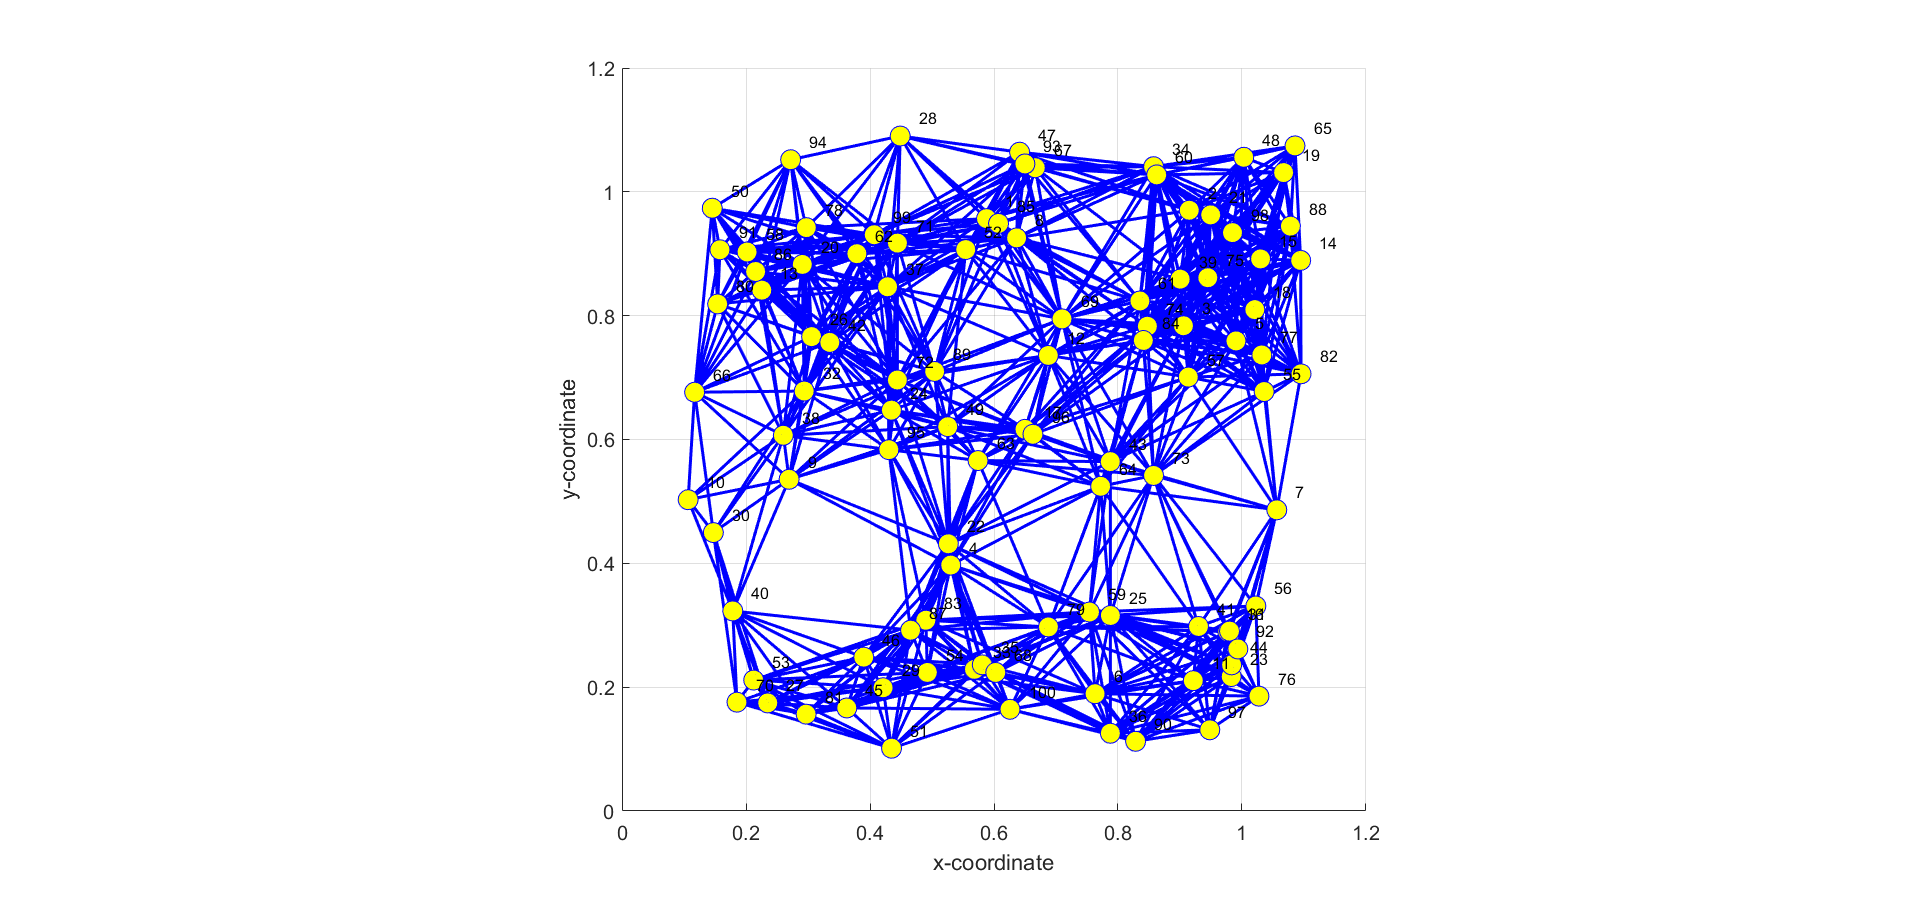
\includegraphics[width=16cm]{Net_100Nodes.png}
	\caption{شبکه‌ای با 100 گره}
	\label{net100}
\end{figure*}



\begin{figure*}[!h]
	\centering
	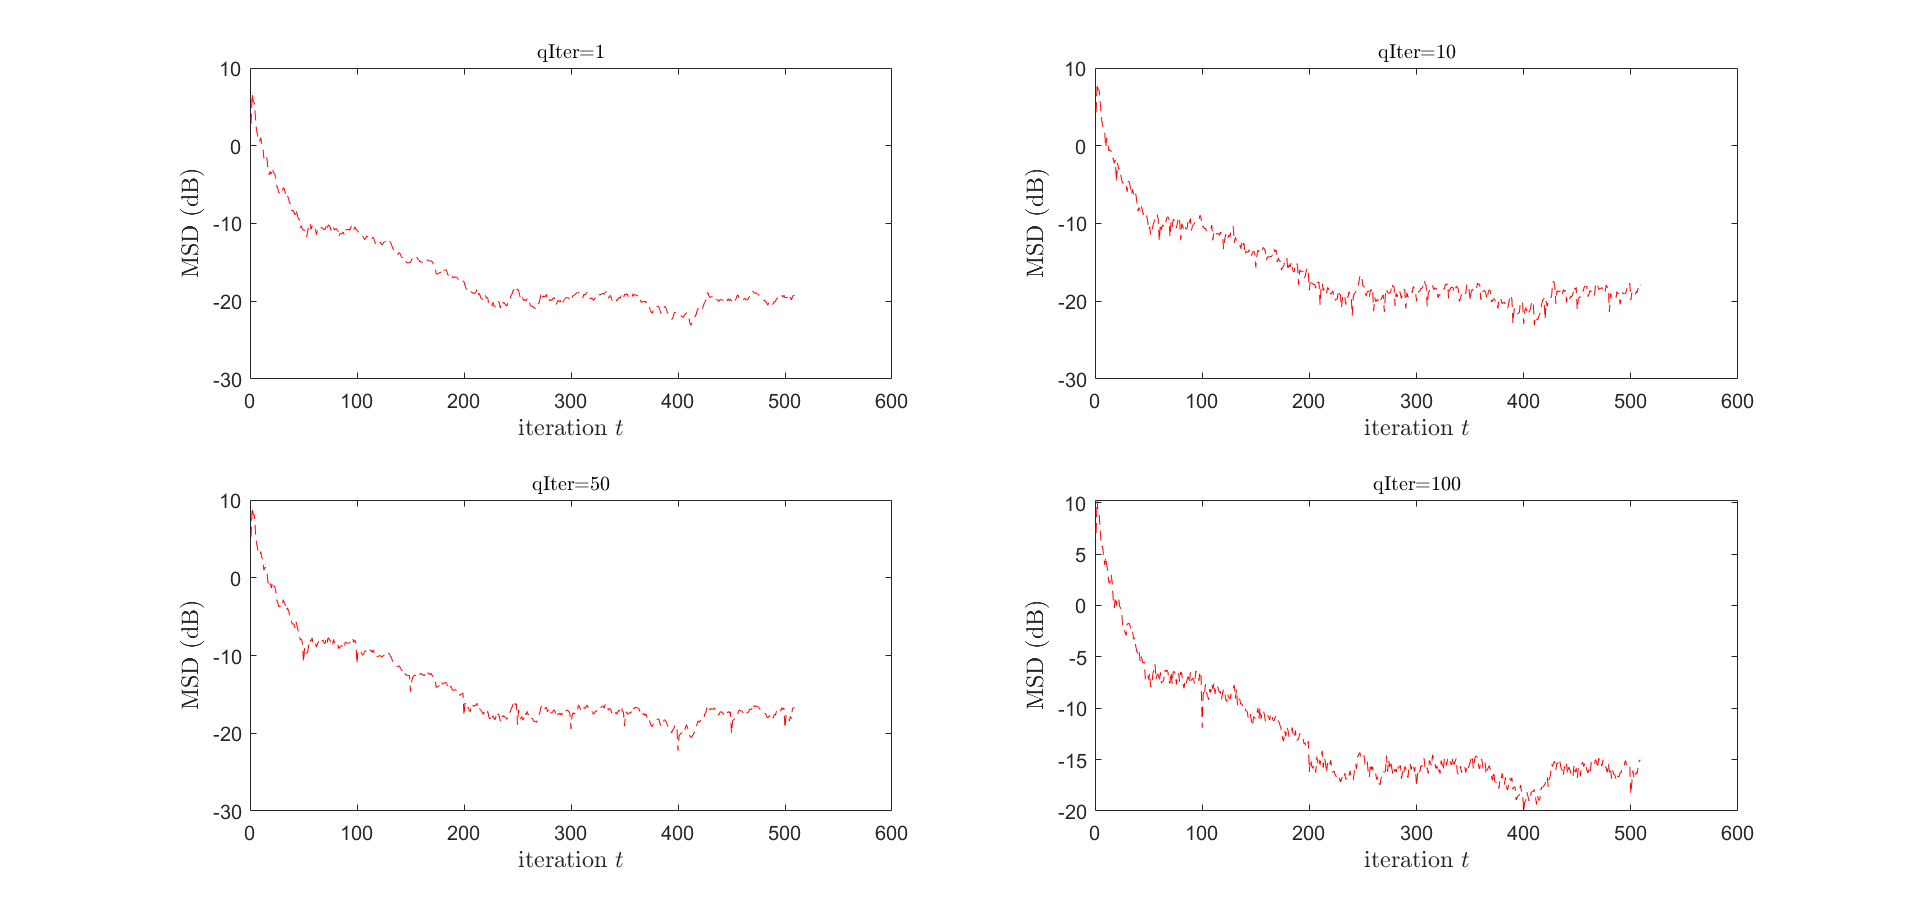
\includegraphics[width=18cm]{FBSP_MixGaussian_500.png}
	\caption{رفتار همگرایی رویکرد پیشنهادی  به ازای مقادیر مختلف پارامتر کنترلی ر یک محیط غیرایستا آغشته به نویز گاوسی آمیخته}
	\label{qIter1}
\end{figure*}
جدول \ref{TableQIter} میانگین زمان انتظار گره‌ها، میانگین مربعات انحراف در حالت پایدار و میانگین تبادلات انجام شده توسط گره‌ها در رویکرد پیشنهادی به ازای مقادیر مختلف پارامتر کنترلی با نماد $qIter$ بر روی $500$ تکرار در یک محیط غیرایستا آغشته به نویز گاوسی آمیخته را نشان می‌دهد. همان طور که دیده می‌شود، اجرای ابرگام‌های منطقه‌ای باعت می‌شود در حالت پایدار رویکرد پیشنهادی به میانگین خطای بالاتری همگرا ‌شود اما قادر است تاثیر بسیار مطلوبی بر کاهش زمان انتظار گره‌ها داشته باشد. به طور میانگین این رویکرد به ترتیب منجر به کاهش $34/67\%$، $63.1\%$ و $70.57\%$ زمان انتظار گره‌ها به ازای مقادیر $qIter=10$، $qIter=50$ و $qIter=100$ می‌شود. همچنین این رویکرد قادر است سبب کاهش $27.83\%$ و $36.73\%$ و $50.37\%$ در تعداد ارتباطات به ترتیب به ازای مقادیر $qIter=10$، $qIter=50$ و $qIter=100$ شود.
\begin{table}
	\centering
	\caption{رفتار رویکرد پیشنهادی به ازای مقادیر مختلف پارامتر کنترلی }\label{TqIter}
	\begin{tabular}{|c|c|c|c|}\hline
		\lr{Avg. Num. of Comm. per iter.}&\lr{Avg. Idle Time(s)} & \lr{MSD(dB)}& \lr{Approach}  \\\hline
		$20.23$ & $30$ & $-19.27$  & \lr{FBSP with qIter=1}\\\hline
		$14.6$ &  $19.6$ & $-17.93$& \lr{FBSP with qIter=10}\\\hline
		$11.8$ & $11.07$  & $-16.69$&\lr{FBSP with qIter=50}\\\hline
		$10.04$ & $8.83$  & $-15.03$ & \lr{FBSP with qIter=100}\\\hline
	\end{tabular}
	\label{TableQIter}
\end{table}
با افزایش مقدار پارامتر کنترلی $qIter$ تعداد دفعات اجرای ابرگام سراسری در طول اجرای فرآیند یادگیری توزیع‌شده و به دنبال آن ارتباطات و تبادلات سراسری گره‌ها کمتر خواهد شد. دریافت اطلاعات توسط یک گره از کلیه گره‌های همسایه (ارتباطات سراسری) در مرحله ترکیب یادگیری توزیع‌شده انتشاری به همگرایی سریع‌تر به خطای کمتر در حالت پایدار کمک می‌کند. اما با این آزمایش  بررسی شد که اگر برقراری ارتباطات سراسری توسط هر گره به یک بار به ازای $qIter$ بار برقراری ارتباطات منطقه‌ای  کاهش یابد، نتایج قابل قبولی بر اساس معیارهای میانگین زمان انتظار گره‌ها، انحراف میانگین مربعات در حالت پایدار و میانگین تبادلات انجام شده حاصل خواهد شد (جدول \ref{TableQIter} را ببینید). همان طور که در شکل \ref{qIter1} نشان داده شده است، در طی فرآیند یادگیری توزیع‌شده در تکرارهایی که ابرگام سراسری اجرا می‌شود پیک‌هایی در منحنی \lr{MSD} دیده می‌شود و بعد از چند تکرار منحنی بر اساس نتایج بدست آمده از تبادلات سراسری روند قبلی خود را با تمایل به خطا کمتر ادامه خواهد داد. این آزمایش برای محیط‌ غیرایستا آغشته به نویز گاوسی و محیط غیرایستا آغشته به نویز آلفا-پایدار نیز تکرار شد و منحنی \lr{MSD} آن‌ها به ترتیب در شکل‌های \ref{qIter2} و \ref{qIter3} نشان داده شده است. 

\begin{figure*}[!h]
	\centering
	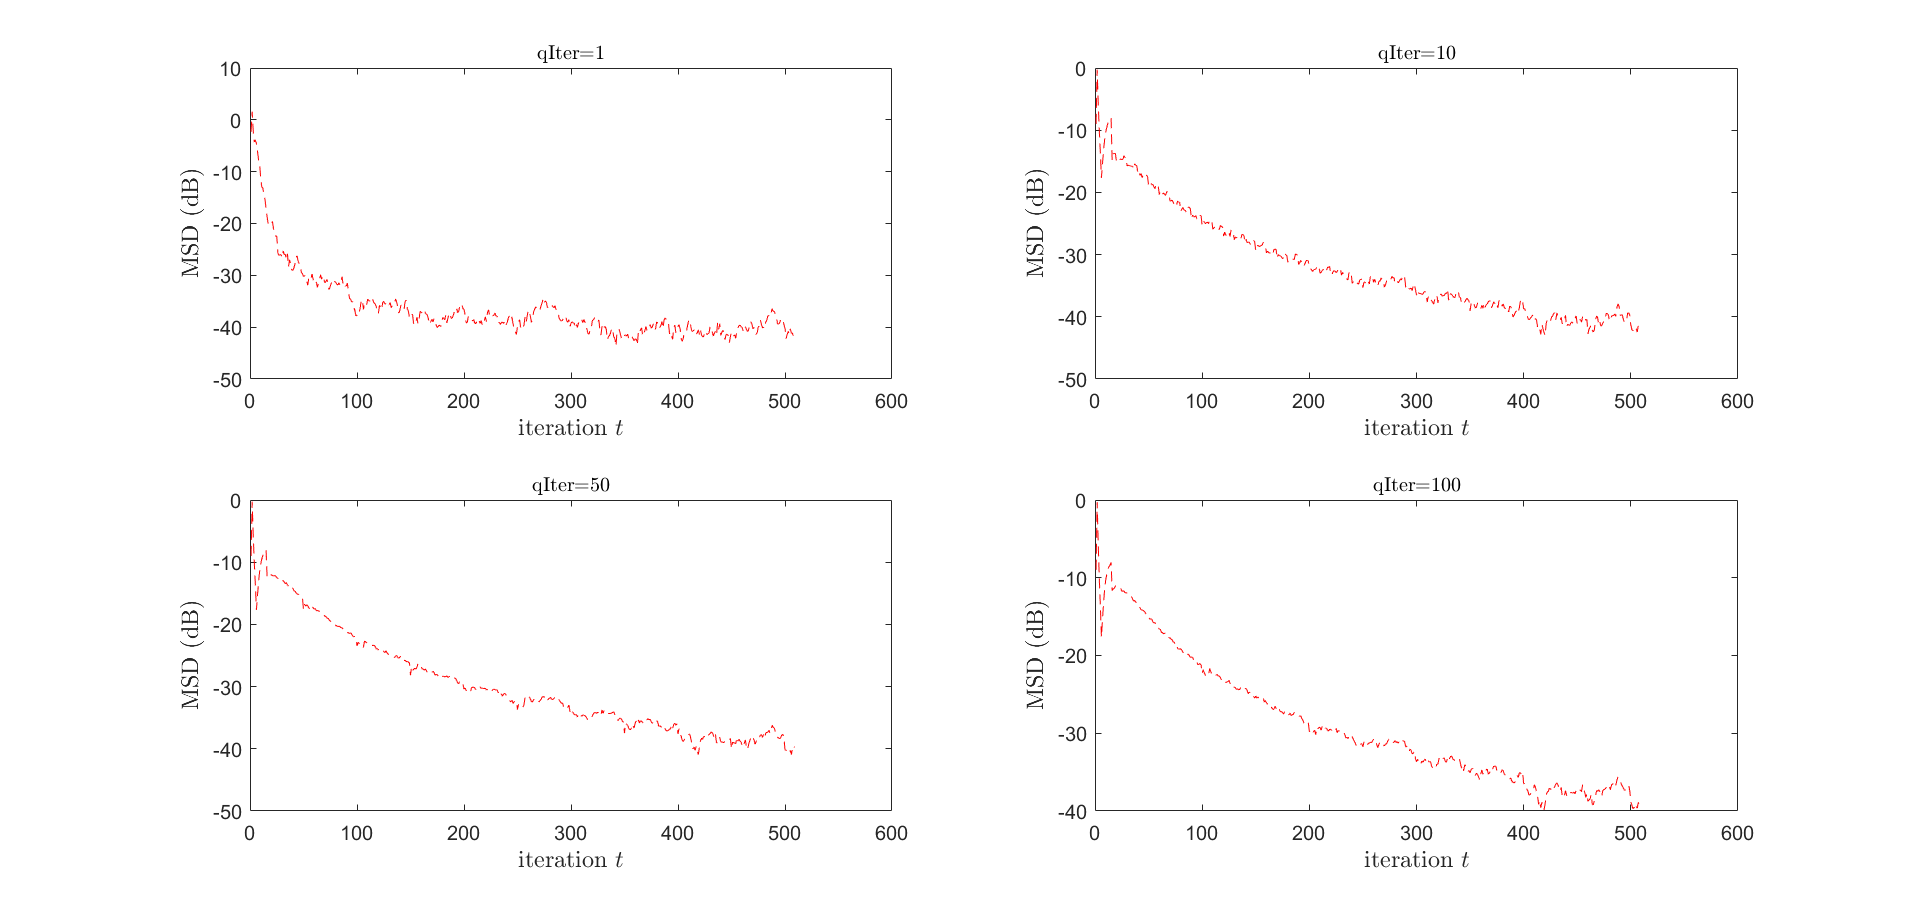
\includegraphics[width=18cm]{FBSP_Gaussian_500_.png}
	\caption{رفتار همگرایی رویکرد پیشنهادی  به ازای مقادیر مختلف پارامتر کنترلی در یک محیط غیرایستا آغشته به نویز گاوسی}
	\label{qIter2}
\end{figure*}

\begin{figure*}[!h]
	\centering
	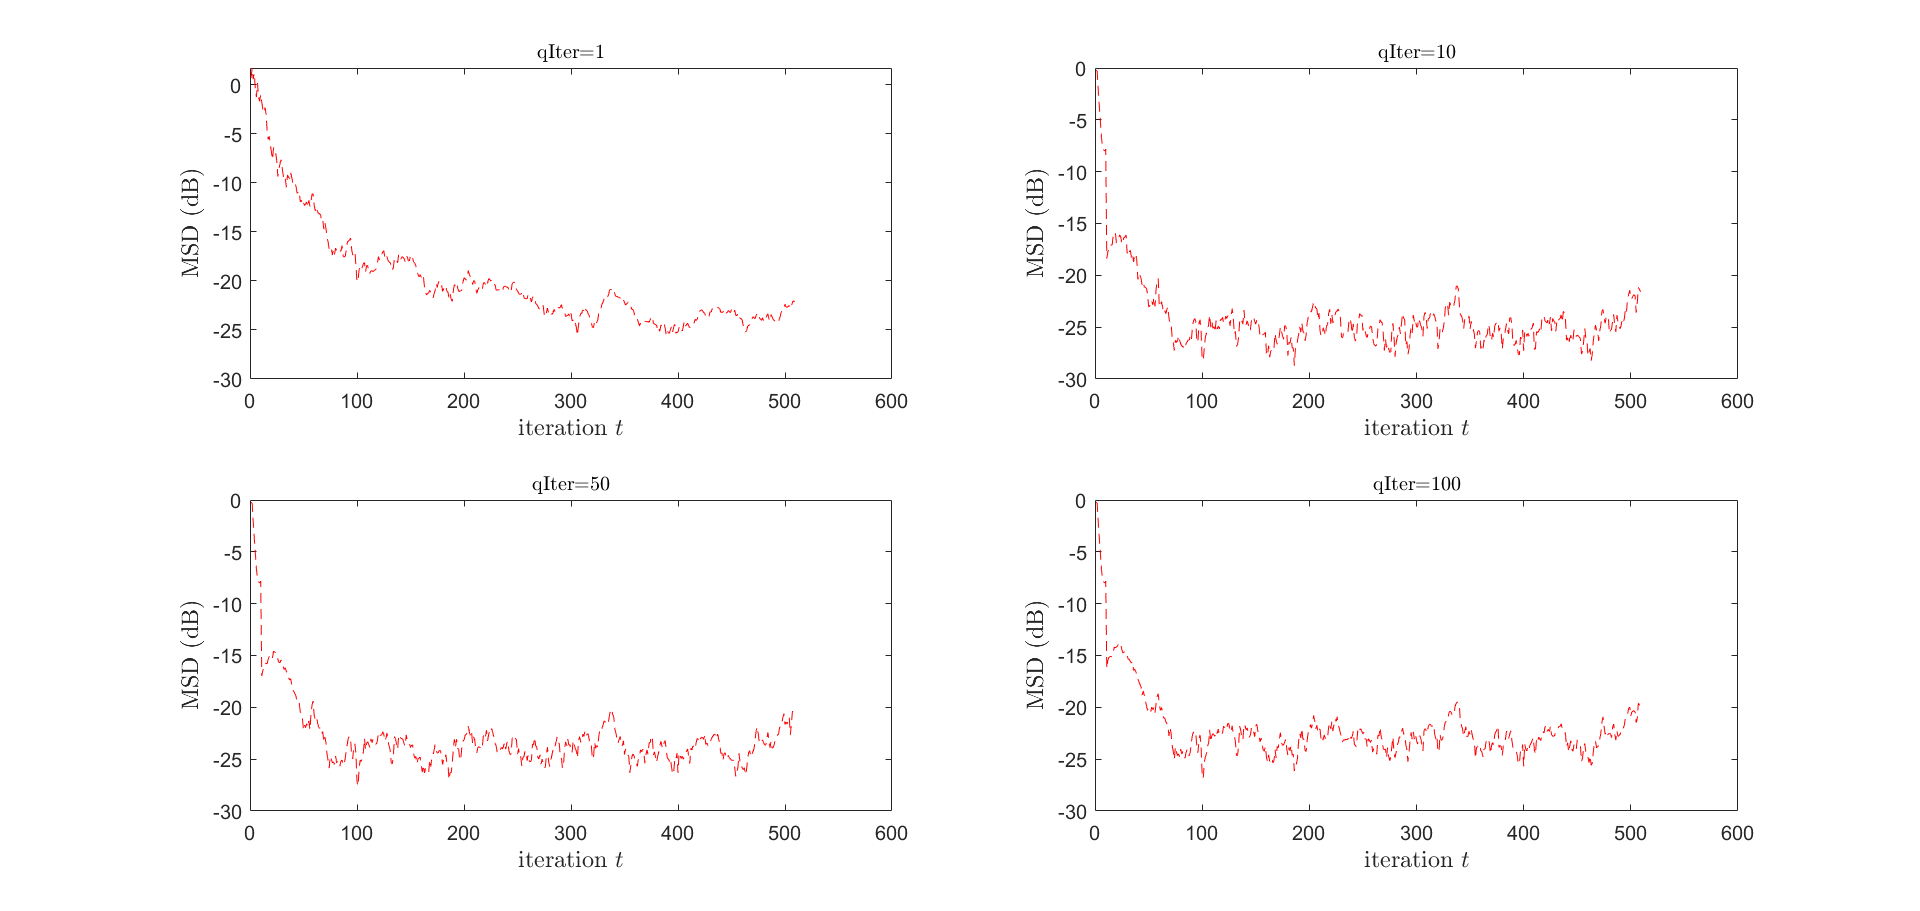
\includegraphics[width=18cm]{FBSP_Alpha_500.png}
	\caption{رفتار همگرایی رویکرد پیشنهادی  به ازای مقادیر مختلف پارامتر کنترلی در یک محیط غیرایستا آغشته به نویز آلفا-پایدار}
	\label{qIter3}
\end{figure*}

در آزمایش دوم میانگین زمان انتظار گره‌ها و انحراف میانگین مربعات در رویکرد پیشنهادی در دو حالت $qIter=1$ و $qIter=50$ با سه رویکرد یادگیری توزیع‌شده \lr{RNA}، \lr{Synch-Switch} و \lr{PSP} در سه محیط غیرایستا آغشته به نویز گاوسی آمیخته، گاوسی و آلفا-پایدار مقایسه شده است. نتایج مقایسه رویکرد پیشنهادی \lr{FBSP} با سه رویکرد دیگر از حیث میانگین زمان انتظار گره‌ها در زمان همگام‌سازی در شکل \ref{Idle1} نشان داده شده است. همان طور که دیده می‌شود، زمان انتظار گره‌ها در رویکرد \lr{FBSP} با پارامتر کنترلی $qIter=1$ (در این حالت \lr{FBSP} تقریبا مشابه \lr{BSP} رفتار می‌کند) از کلیه رویکردهای مورد مقایسه بیشتر است. این اختلاف زیاد به این دلیل است که تمام همگام‌سازی‌ها در \lr{FBSP} با پارامتر $qIter=1$ به صورت همگام‌سازی سراسری اجرا می‌شوند. رویکرد \lr{RNA} در هر ابرگام زمان اتمام کار تنها یک گره نماینده تصادفی را ملاک زمان اجرای همگام‌سازی قرار می‌دهد و به همین دلیل میانگین زمان انتظار گره‌ها در این رویکرد کمتر از سایر رویکردهای مورد مقایسه است. در این آزمایش \lr{FBSP} با پارامتر $qIter=50$ از لحاظ زمان انتظار تقریبا مشابه رویکرد \lr{PSP} عمل می‌کند. در رویکرد \lr{PSP} زمان همگام‌سازی گره‌ها بر اساس زمان اتمام کار محاسباتی حداقل $20$ درصد از گره‌ها تعیین می‌گردد که این گره‌ها به صورت تصادفی انتخاب می‌شوند.

\begin{figure*}[!h]
	\centering
	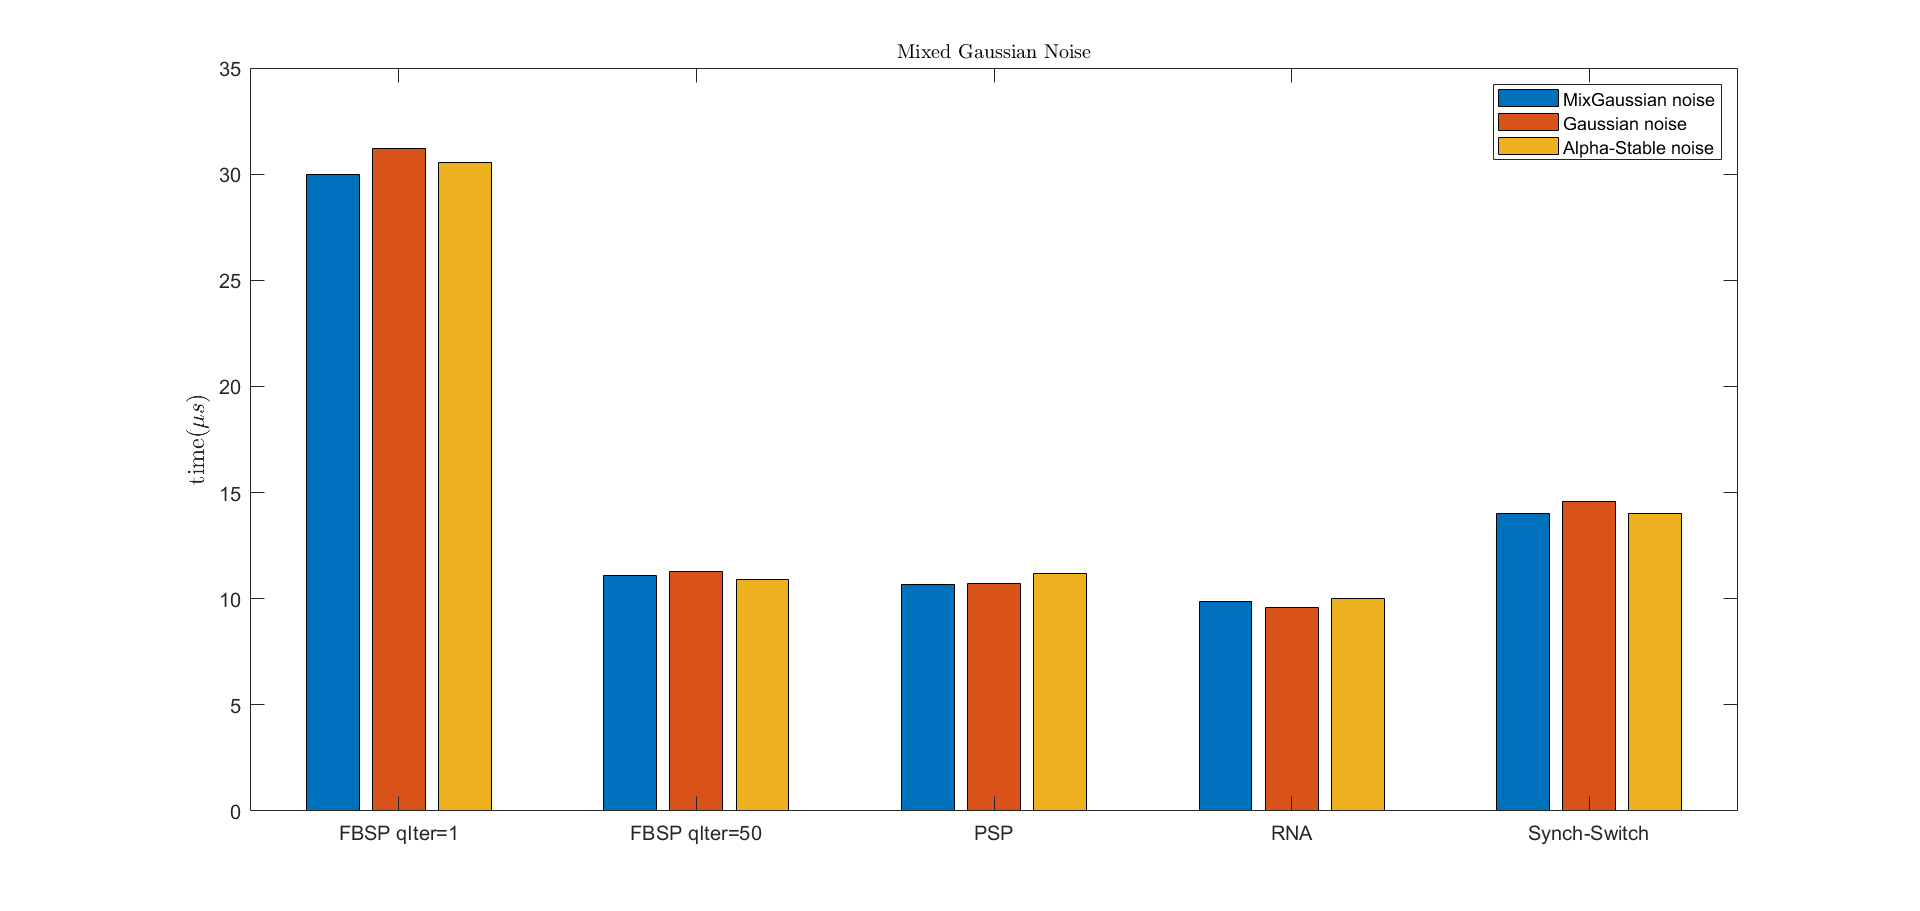
\includegraphics[width=18cm]{IdleTime_All.png}
	\caption{مقایسه زمان انتظار گره‌ها در رویکرد پیشنهادی با سایر رویکردهای یادگیری توزیع‌شده مشابه}
	\label{Idle1}
\end{figure*}
همچنین در شکل \ref{Idle2} انحراف میانگین مربعات در حالت پایدار رویکرد پیشنهادی با رویکردهای یادگیری توزیع‌شده مشابه در سه محیط غیرایستا آغشته به نویز گاوسی آمیخته، گاوسی و آلفا-پایدار مقایسه شده است. شکل \ref{Idle2} نشان می‌دهد که رویکرد \lr{FBSP} با پارامتر $qIter=1$ قادر است در حضور هر سه نوع نویز محیطی به خطا کمتری نسبت به سایر رویکردها همگرا می‌شود. رویکرد \lr{FBSP} با پارامتر کنترلی $qIter=50$ در موقعیت دوم نسبت به سایر رویکردهای مورد مقایسه قرار دارد که البته با توجه به نتایج ارائه شده در شکل \ref{Idle1} و با در نظر گرفتن توانایی رویکرد \lr{FBSP} با پارامتر کنترلی $qIter=50$ در کاهش زمان انتظار گره‌ها در طی فرآیند یادگیری، می‌توان ادعا کرد که نتایج انحراف میانگین مربعات در حالت پایدار قابل قبول می‌باشند. در نتیجه اختلاف کمی که بین  نتایج \lr{MSD} حالت پایدار رویکرد پیشنهادی در حالت  $qIter=50$ و $qIter=1$ دیده می‌شود، قابل چشم‌پوشی است. رویکرد \lr{RNA} به دلیل استناد به اتمام کار تنها یک گره تصادفی در هر ابرگام و به احتمال زیاد تبادل و استفاده از داده‌های کهنه و ناهماهنگی توسط گره‌های شبکه به مقادیر خطا بیشتری در حالت پایدار همگرا می‌شود. جدول \ref{AllTableFBSP} به طور خلاصه نتایج مقایسه رویکرد پیشنهادی با سایر رویکردهای مشابه را در محیط غیرایستا و در حضور نویز گاوسی آمیخته، نویز گاوسی و نویز آلفا-پایدار نشان می‌دهد. 

\begin{figure*}[!ht]
	\centering
	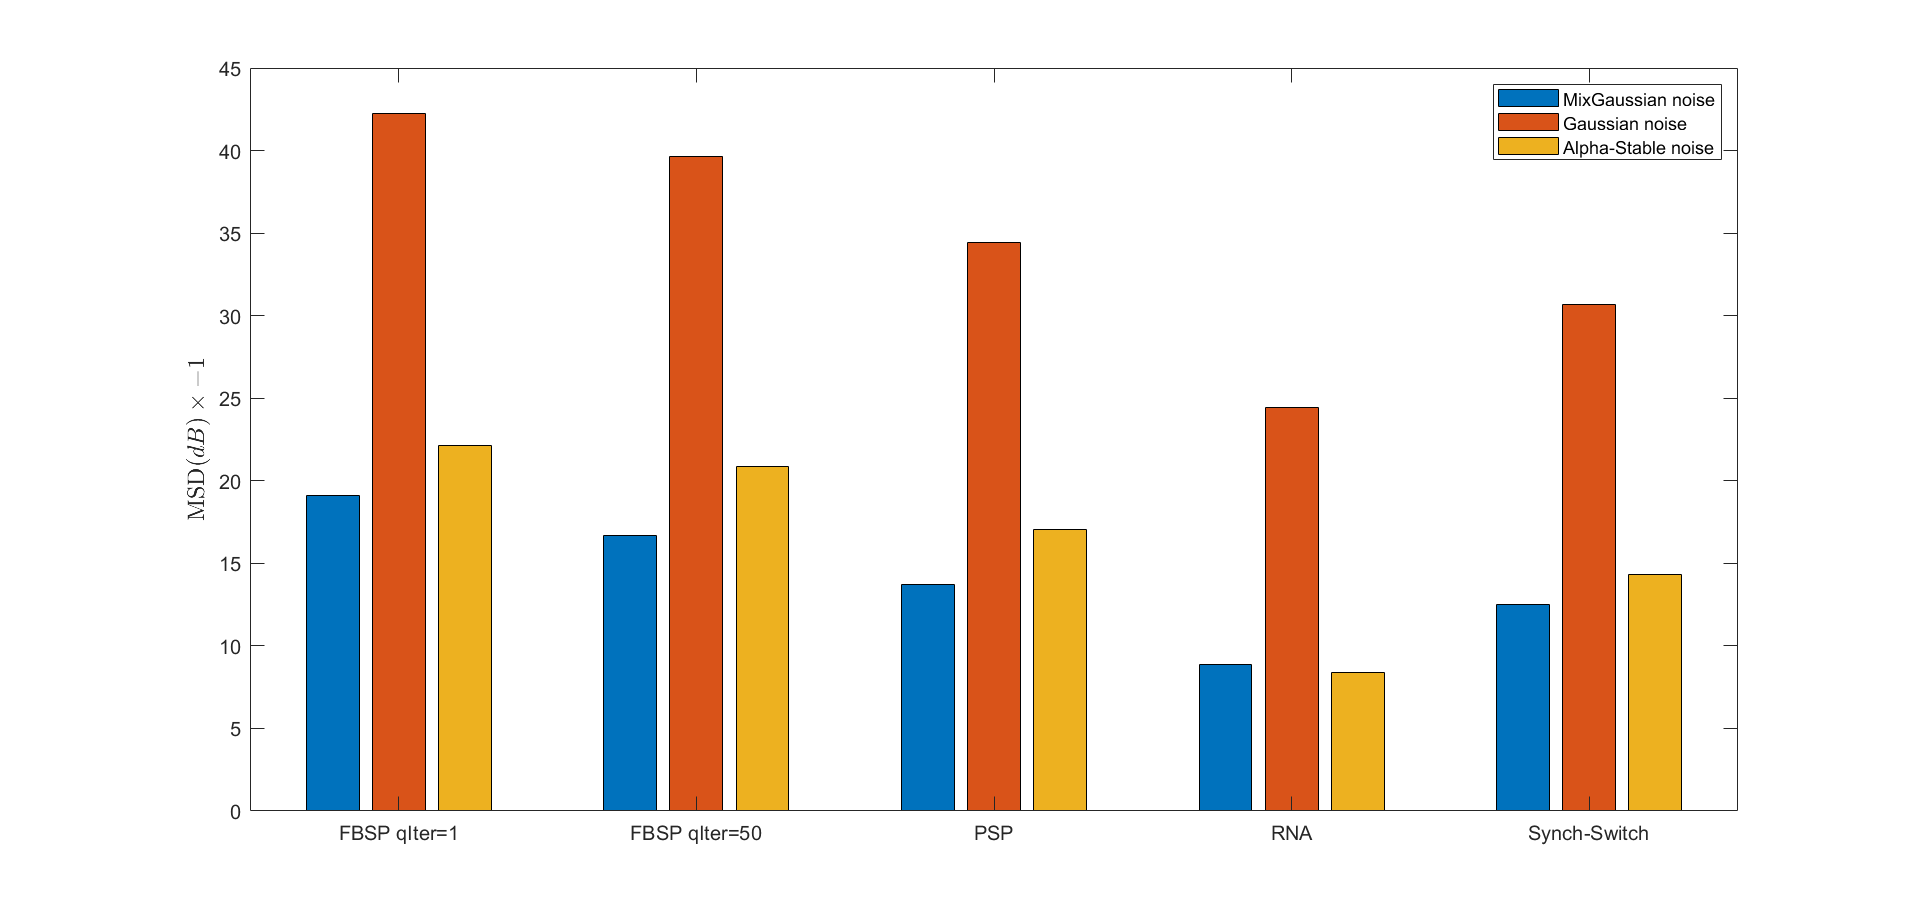
\includegraphics[width=18cm]{MSD_All.png}
	\caption{مقایسه انحراف میانگین مربعات رویکرد پیشنهادی با سایر رویکردهای یادگیری توزیع‌شده مشابه}
	\label{Idle2}
\end{figure*}

\begin{table}[!ht]
	\centering
	\caption{مقایسه رفتار رویکرد پیشنهادی با سایر رویکردهای مشابه}
	\begin{tabular}{|c|c|c|c|c|c|l|}
		\hline
		\multicolumn{2}{|c|}{\lr{Alpha-Stable}} & \multicolumn{2}{|c|}{\lr{Gaussian}} & \multicolumn{2}{|c|}{\lr{MixGaussian}} & \multirow{2}{*}{\lr{Approach}}\\
		\lr{Idle Time(s)} & \lr{MSD(dB)} & \lr{Idle Time(s)} & \lr{MSD(dB)} &\lr{Idle Time(s)} & \lr{MSD(dB)} & \\
		\hline
		$30.53$ & $-22.12$ & $31.2$ & $-42.25$ & $30$ & $-19.27$ & \lr{FBSP with qIter=1}\\\hline
		$10.89$ & $-20.86$ & $11.3$ & $-39.66$ & $11.07$  & $-16.69$&\lr{FBSP with qIter=50}\\\hline
		$10$ & $-8.4$ & $9.60$ & $-24.44$ & $9.883$  & $-8.86$ & \lr{RNA}\\\hline
		$14$ & $-14.3$ & $14.6$ & $-30.68$ & $14.03$  & $-12.5$ & \lr{Synch-Switch}\\\hline
		$11.2$ & $-17.06$ & $10.72$ & $-34.45$ & $10.65$  & $-13.71$ & \lr{PSP}\\\hline
	\end{tabular}
	\label{AllTableFBSP}
\end{table}

در آزمایشی دیگر مقاومت رویکرد پیشنهادی در برابر محیط‌های ناهمگن با سایر رویکردها مورد بررسی و مقایسه قرار گرفته است. در این آزمایش میزان کندی گره‌های شبکه در آزمایش قبلی به $2$ برابر $2\times$ و $10$ برابر $10\times$ تغییر داده می‌شود تا مقاومت رویکردهای یادگیری توزیع‌شده در برابر محیط‌های ناهمگن مختلف ارزیابی گردد. شکل \ref{Robust_Heterogeneous} رفتار همگرایی رویکرد \lr{FBSP} با پارامتر کنترلی $qIter=50$ در $500$ تکرار را در محیط‌های مختلف ناهمگن در مقایسه با سه رویکرد \lr{RNA}، \lr{PSP} و \lr{Synch-Switch} در یک محیط غیرایستا آغشته به نویز گاوسی آمیخته نشان می‌دهد. 

\begin{figure*}[!ht]
	\centering
	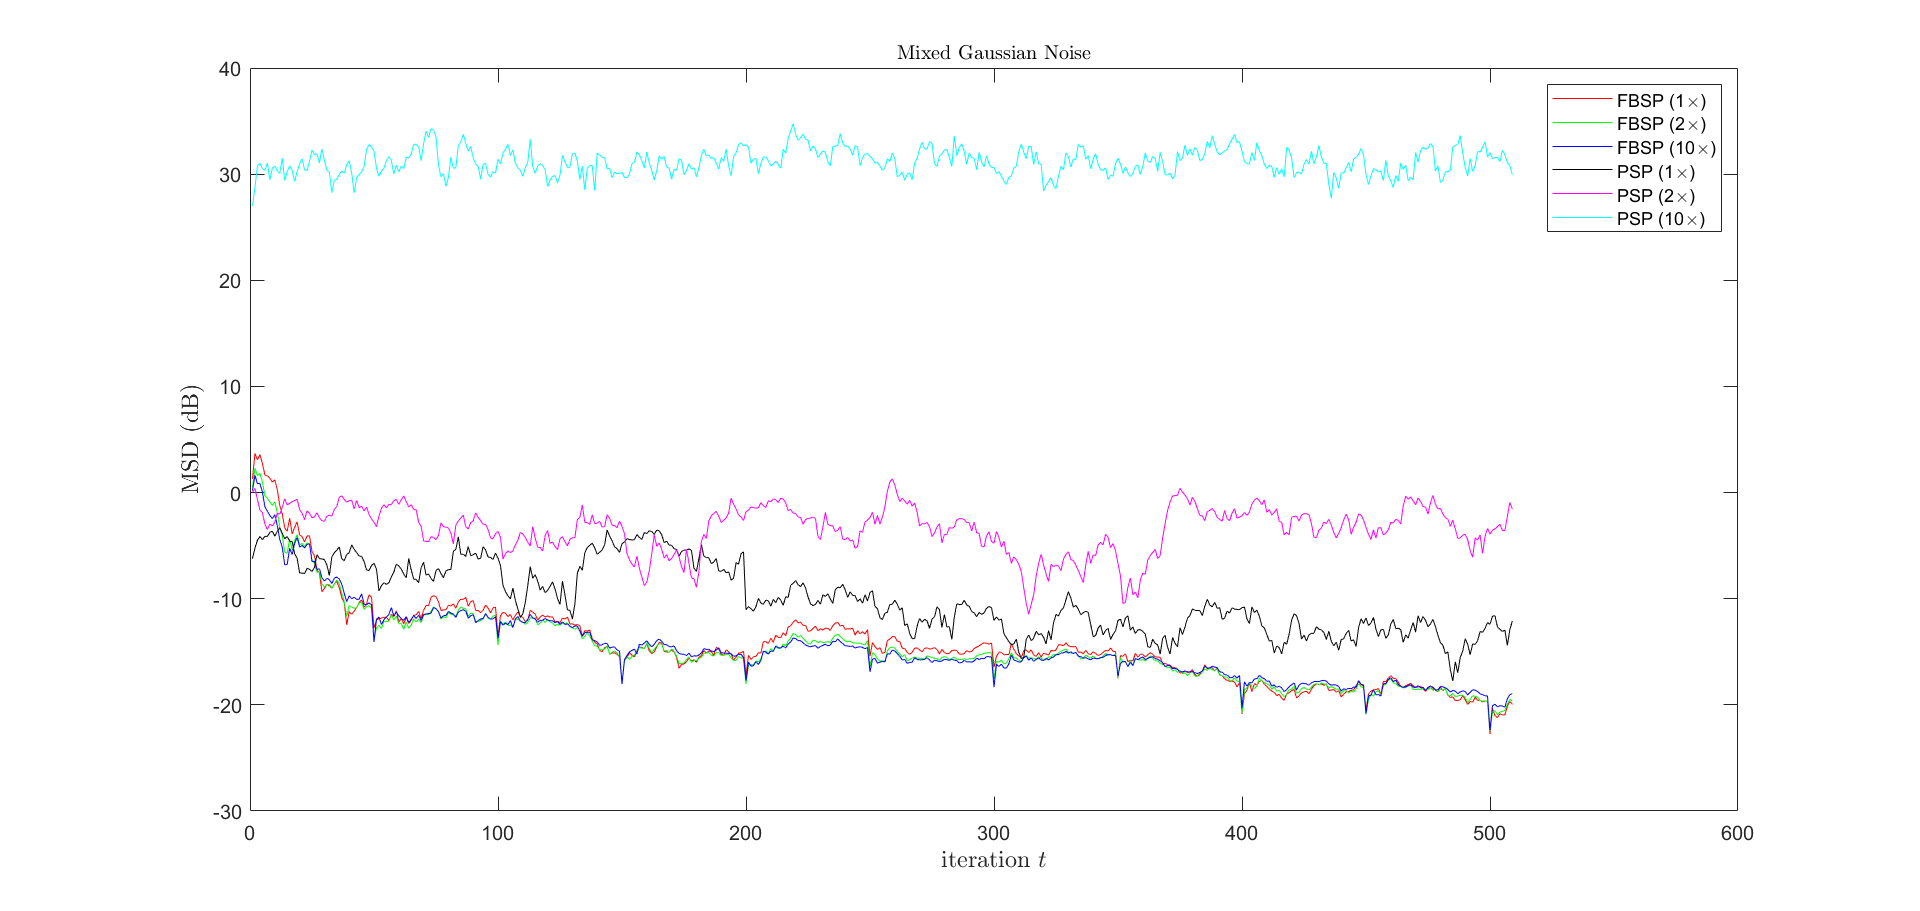
\includegraphics[width=17cm]{Heterogenous.png}
	\caption{مقاومت رویکرد یادگیری توزیع‌شده در محیط‌های ناهمگن مختلف}
	\label{Robust_Heterogeneous}
\end{figure*}

همان طور که مشاهده می‌شود، رویکرد پیشنهادی \lr{FBSP} در برابر درجه ناهمگنی‌های مختلف محیط اجرایی مقاوم است و رفتار همگرایی آن در حالت‌های $1X$، $2X$ و $10X$ تقریبا یکسان می‌باشد. در این آزمایش مقاومت رویکرد یادگیری توزیع‌شده \lr{PSP} که نسبت به دو رویکرد مورد مقایسه دیگر نتایج بهتر و نزدیک‌تری به \lr{FBSP} ارائه می‌دهد، مورد بررسی قرار گرفت. نتایج ارائه شده در \ref{Robust_Heterogeneous} دلالت بر عدم مقاومت رویکرد \lr{PSP} در برابر محیط‌های اجرایی با درجه ناهمگنی مختلف دارند. در نتیجه رویکرد پیشنهادی \lr{FBSP} علاوه بر توانایی در کاهش زمان انتظار گره‌ها و کاهش تعداد ارتباطات، در برابر محیط‌های اجرایی  با درجه ناهمگنی مختلف نیز مقاوم است. 

\subsection{ارزیابی رویکرد یادگیری توزیع‌شده \lr{FBSP} در مساله پیش‌‌بینی بازار بورس}
در سال‌های اخیر، پیش‌بینی بازار سهام موضوع بسیار مهمی برای محققان بوده و مطالعات متعددی برای پیش‌بینی حرکت بازار سهام با استفاده از الگوریتم‌های مختلف یادگیری ماشین انجام شده است. بازار سهام با نوسانات شدید، غیرخطی بودن و تغییرات زیاد متغیرهای محیطی توصیف می‌شود. دلایل مختلفی پشت نوسانات، خطی نبودن بازار سهام وجود دارد، از جمله گرانی سهام شرکت، گزارش زیان شرکت، جنگ تجاری، رکود بازار جهانی، تنش‌های ژئوپلیتیکی و بیماری‌های همه‌گیر مانند ویروس کرونا را می‌توان ذکر کرد.

در این بخش یک مجموعه از داده‌های بورس ایران شامل اطلاعات 736 شرکت مورد استفاده قرار گرفته است. در این مجموعه داده، اطلاعات هر شرکت به صورت یک ساختار داده به شرح زیر در دسترس می‌باشد:
\begin{itemize}
	\item \lr{Name}: نام كامل شرکت
	\item \lr{Namad}: نام مختصر یا معروف شرکت
	\item \lr{Data}: برداری از اطلاعات مختلف مربوط به شرکت 
	\item  \lr{HDate}: تاریخ روزهایی که اطلاعات مربوط به آنها در بردار \lr{Data} وجود دارد
	\item \lr{HPrice}: ساختار داده‌ای که شامل اطلاعات مختلف مربوط به قیمت شرکت موردنظر در هر كدام از
	روزها در \lr{HDate}
	\begin{itemize}
		\item \lr{High}: بالاترین قیمت هر سهم در هر روز
		\item  \lr{Low}: کمترین قیمت سهم در هر روز
		\item \lr{Close}: میانگین وزن‌دار قیمت معامله‌های انجام شده در نیم ساعت پایانی روز
		\item \lr{Last}: قیمت اخرین معامله ی انجام شده
		\item \lr{First}: قیمت اولین معامله ی انجام شده
		\item \lr{Open}: میانگین وزن‌دار قیمت معامله‌های انجام شده در نیم ساعت اغازین روز
		\item \lr{ValTrades}: ارزش معاملات
		\item \lr{NumShares}: تعداد سهام
		\item \lr{NumTrades}: تعداد معاملات
		\item \lr{Grad}: گرادیان
		\item \lr{FHigh}: فلیپ شده \lr{High}
		\item \lr{Flow}: فلیپ شده \lr{Low}
		\item \lr{FClose}: فلیپ شده \lr{Close} و غیره
	\end{itemize}
	\item \lr{FHDate}: فلیپ شده \lr{HDate}
	\item \lr{Len}: اطلاعات زمانی مرتبط با داده (تعداد روزهای هفته، ماه و سال و ...)
	\item \lr{RL}: اطلاعات مربوط به حقیقی و حقوقی‌ها	
\end{itemize}



رویکرد \lr{FBSP} با کمک الگوریتم‌های یادگیری توزیع‌شده تطبیقی می‌توانند رفتار غیرخطی در سیگنال‌های بورس را تشخیص داده و به نتایج پیش‌بینی بسیار دقیقی منجر شوند. در این بخش، از الگوریتم \lr{RDSGD} برای پیش‌بینی روز-آینده\footnote{\lr{next-day}} روند سهام استفاده شده است و قابلیت پیش‌بینی رویکرد پیشنهادی بر اساس الگوریتم‌‌های یادگیری توزیع‌شده \lr{RDSGD}، \lr{DLMS}، \lr{DRLS}، \lr{DSGD}، \lr{SGD} و \lr{RDLMS} مورد ارزیابی قرار گرفته است. برای این منظور از مجموعه داده‌های مربوط به معاملات شرکت‌های مختلف در بازار سهام ایران استفاده شده است. آزمایش‌‌ها بر روی یکی از سیگنال‌های ارائه شده در این مجموعه داده به نام \lr{Fclose} انجام می‌شود. این سیگنال میانگین وزن‌دار ارزش تراکنش‌های انجام شده در نیم ساعت آخر روز را نشان می‌دهد. به عنوان نمونه در شکل \ref{Compaies} سیگنال \lr{fclose} شرکت‌های داروسازی کاسپین تامین \lr{Caspian}، شرکت سرمایه‌گذاری ملت \lr{VMelat}، شرکت کشت و صنعت شریف‌آباد \lr{ZSharif} و شرکت پرمیت \lr{Permit} نشان داده شده است.

\begin{figure}[htbp]  \centering{
		\subfigure[]{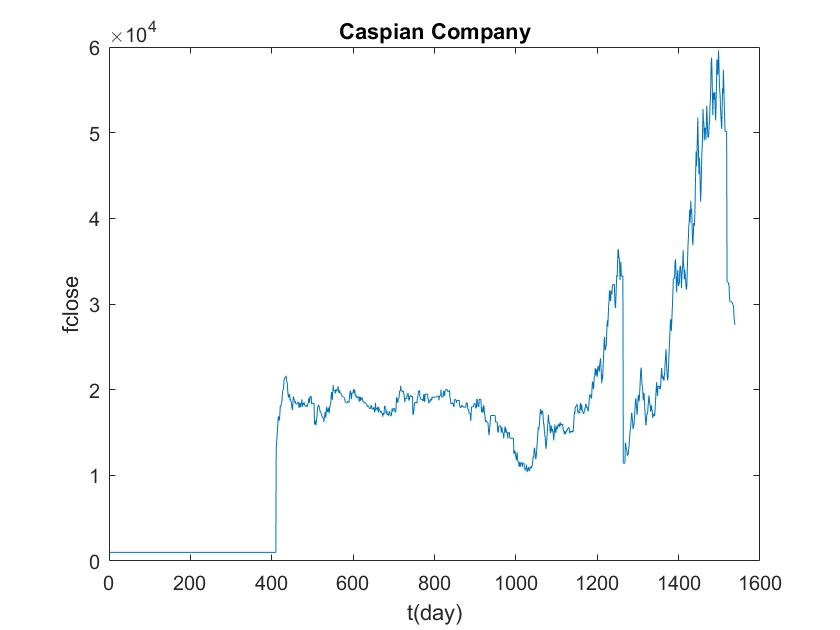
\includegraphics[width=8 cm,height=5 cm]{Caspian.jpg}\label{fig:Caspian}}
		\subfigure[]{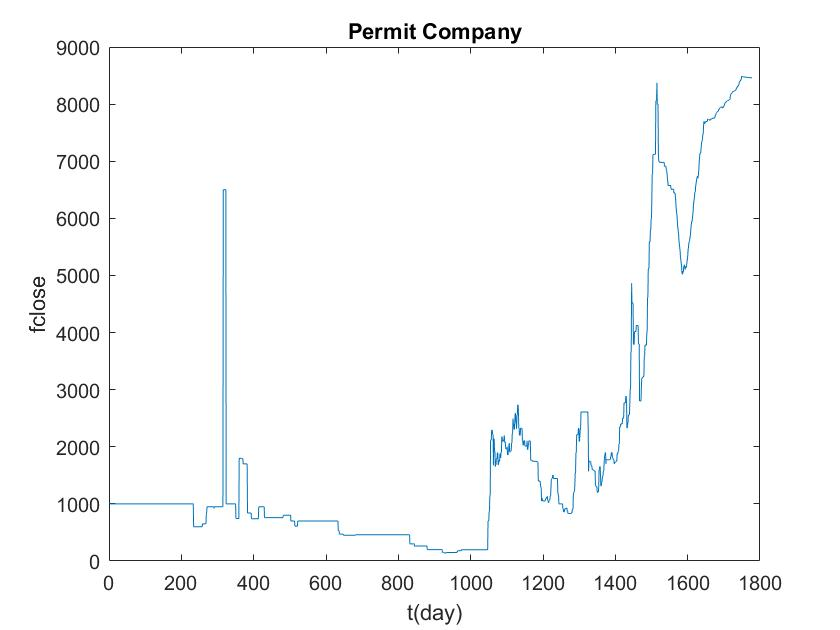
\includegraphics[width=8 cm,height=5 cm]{Permit.jpg}\label{fig:BuAli}}
		\\
		\subfigure[]{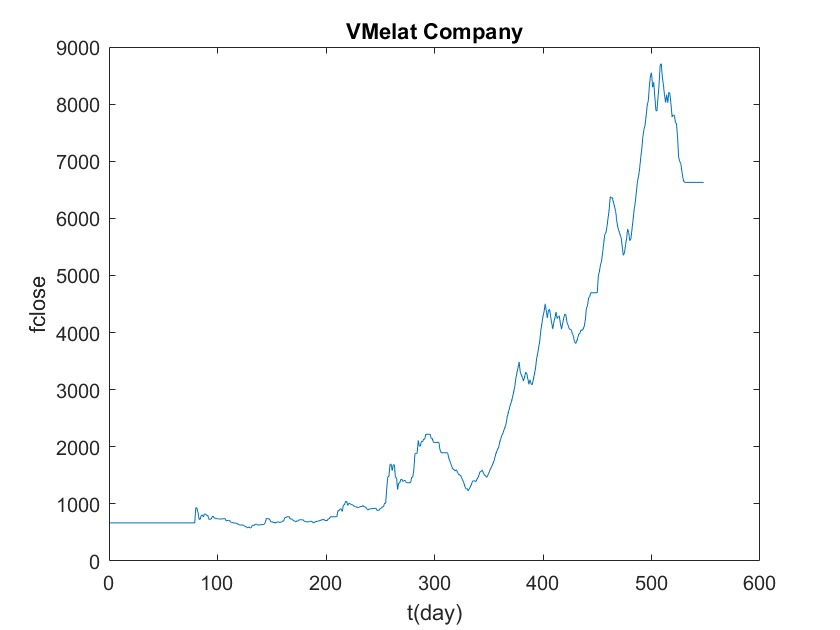
\includegraphics[width=8 cm,height=5 cm]{VMelat_fclose.png}\label{fig:Khazar}}
		\subfigure[]{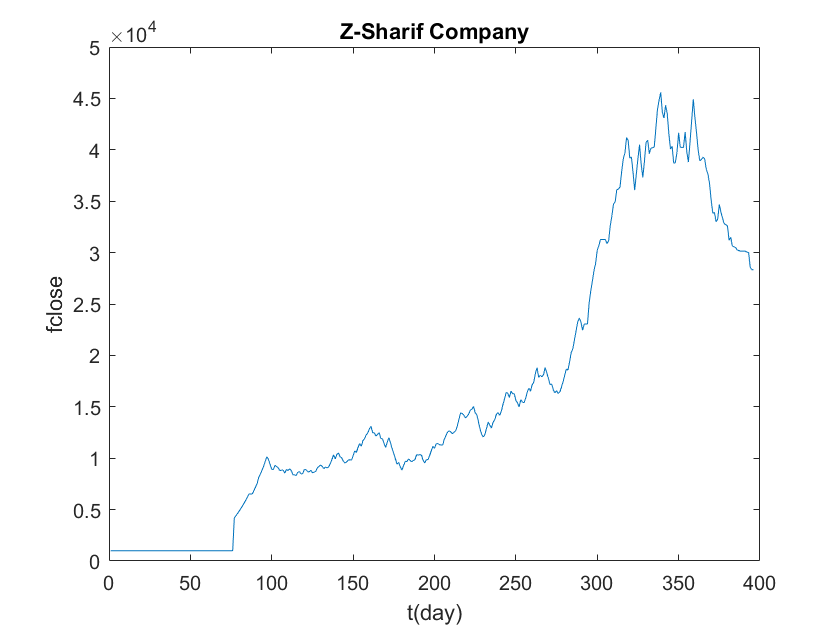
\includegraphics[width=8 cm,height=5 cm]{ZSharif_fclose.png}\label{fig:Permit}}
	}
	\caption[]{سیگنال \lr{Fclose} برخی از شرکت‌ها. الف) \lr{Caspian company}
		ب) \lr{Permit Company}
		ج) \lr{VMelat Company}
		د) \lr{ZSharif Company}
	}
	\label{Compaies}
\end{figure}

هدف از این آزمایش بررسی توانایی الگوریتم‌های یادگیری توزیع‌شده مختلف رویکرد \lr{FBSP} در مساله پیش‌بینی است. با توجه به اینکه ارائه و نمایش منحنی‌های پیش‌بینی شرکت‌های متعدد مجموعه داده موردنظر خارج از حوصله این نوشته است، در این آزمایش تنها به نمایش منحنی پیش‌بینی چند شرکت (ذکر شده در \ref{Compaies}) در ازای شش الگوریتم یادگیری توزیع‌شده اکتفا خواهد شد. در شکل‌های \ref{PredictCompare1} تا \ref{PredictCompare4} توانایی رویکرد پیشنهادی در پیش‌بینی سیگنال \lr{Fclose} شرکت‌های  \lr{Caspian}، \lr{Permit}، \lr{VMelat} و \lr{ZSharif} نشان داده شده است. همان‌طور که دیده می‌شود، الگوریتم‌های \lr{LMS} هم نسخه انتشاری آن (\lr{DLMS}) و هم نسخه انتشاری مقاوم آن (\lr{RDLMS}) قادر به پیش‌بینی سیگنال‌های بازار سهام نمی‌باشند. همچنین، الگوریتم \lr{SGD} شبیه الگوریتم \lr{RDLMS} عمل می‌کند و قادر به پیش‌بینی این سیگنال‌ها نمی‌باشد. الگوریتم \lr{RDSGD}، \lr{DSGD} , \lr{DRLS} در پیش‌بینی سیگنال‌ها موفق‌تر بوده و قادر به پیش‌بینی سیگنال \lr{Fclose} شرکت‌ها با خطای کمتری در مقایسه با الگوریتم‌های دسته \lr{LMS} هستند. \lr{DSGD} در مقایسه با \lr{RDSGD} پیش‌بینی‌ها را با دقت بالاتری ارائه می‌دهد و از این لحاظ مشابه \lr{DRLS} عمل می‌کند.

\begin{figure*}[!h]
	\centering
	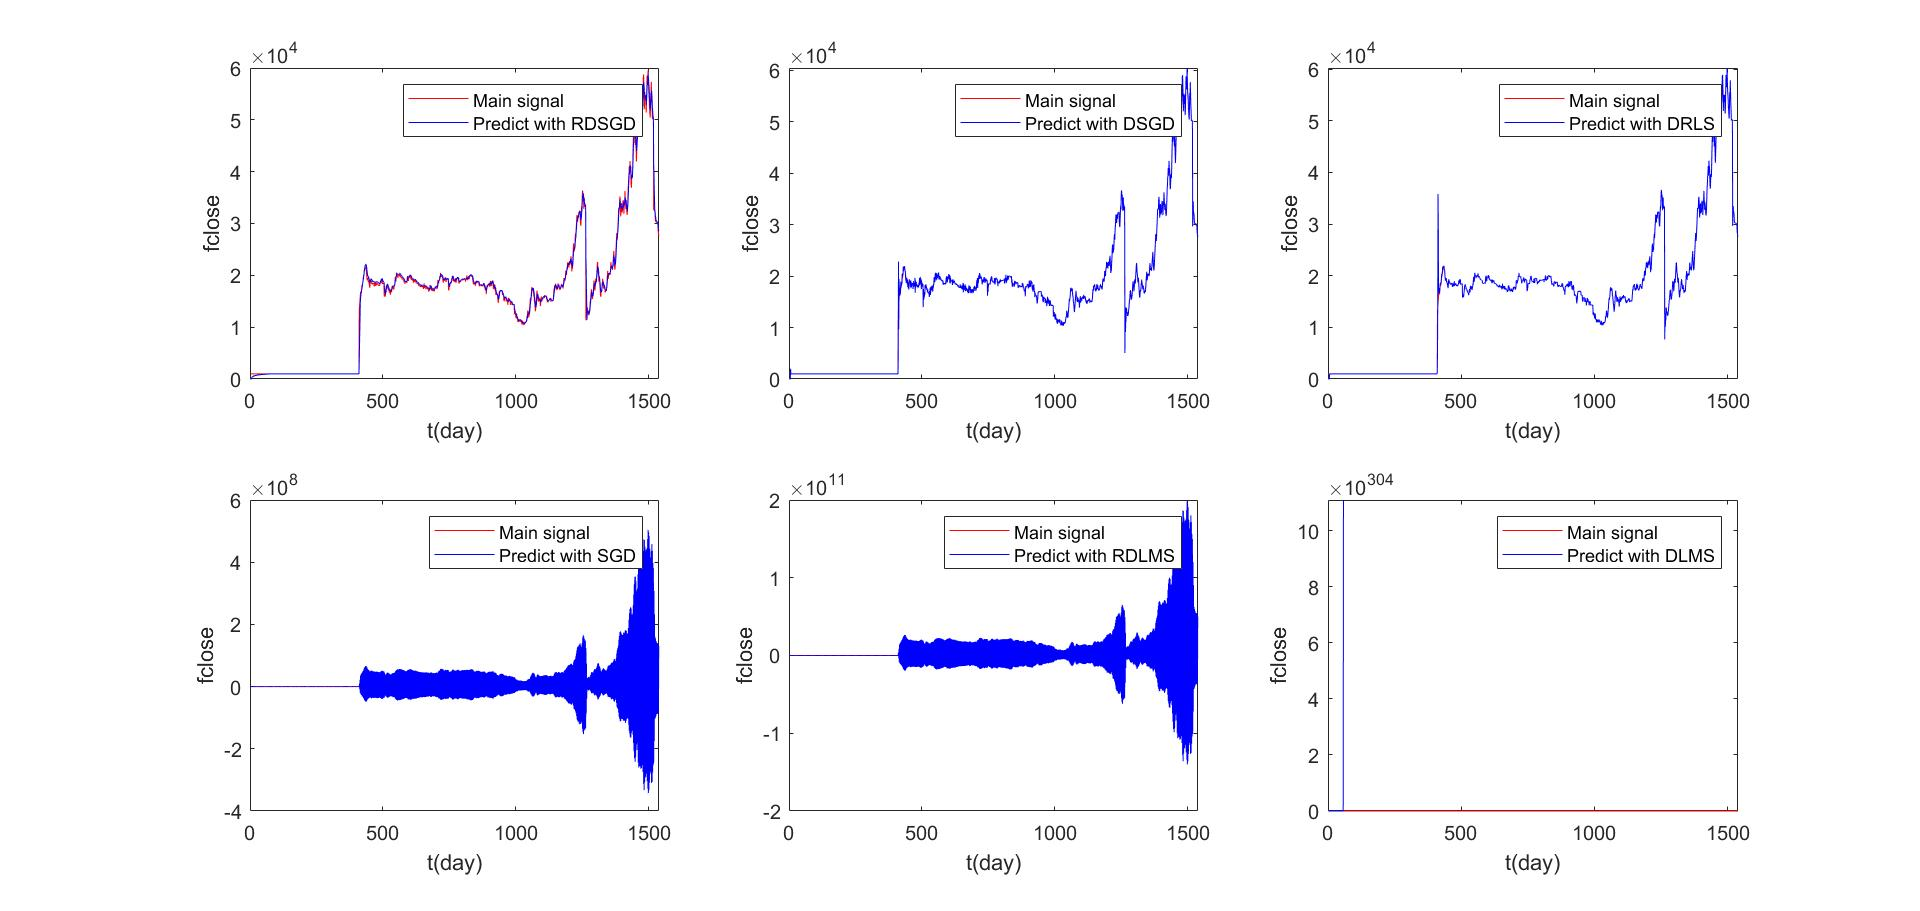
\includegraphics[width=16cm]{CompareFigs_6_Caspian.jpg}
	\caption{مقایسه الگوریتم‌های یادگیری توزیع‌شده رویکرد \lr{FBSP} در پیش‌بینی سیگنال بازار سهام شرکت داروسازی کاسپین تامین}
	\label{PredictCompare1}
\end{figure*}

\begin{figure*}[!h]
	\centering
	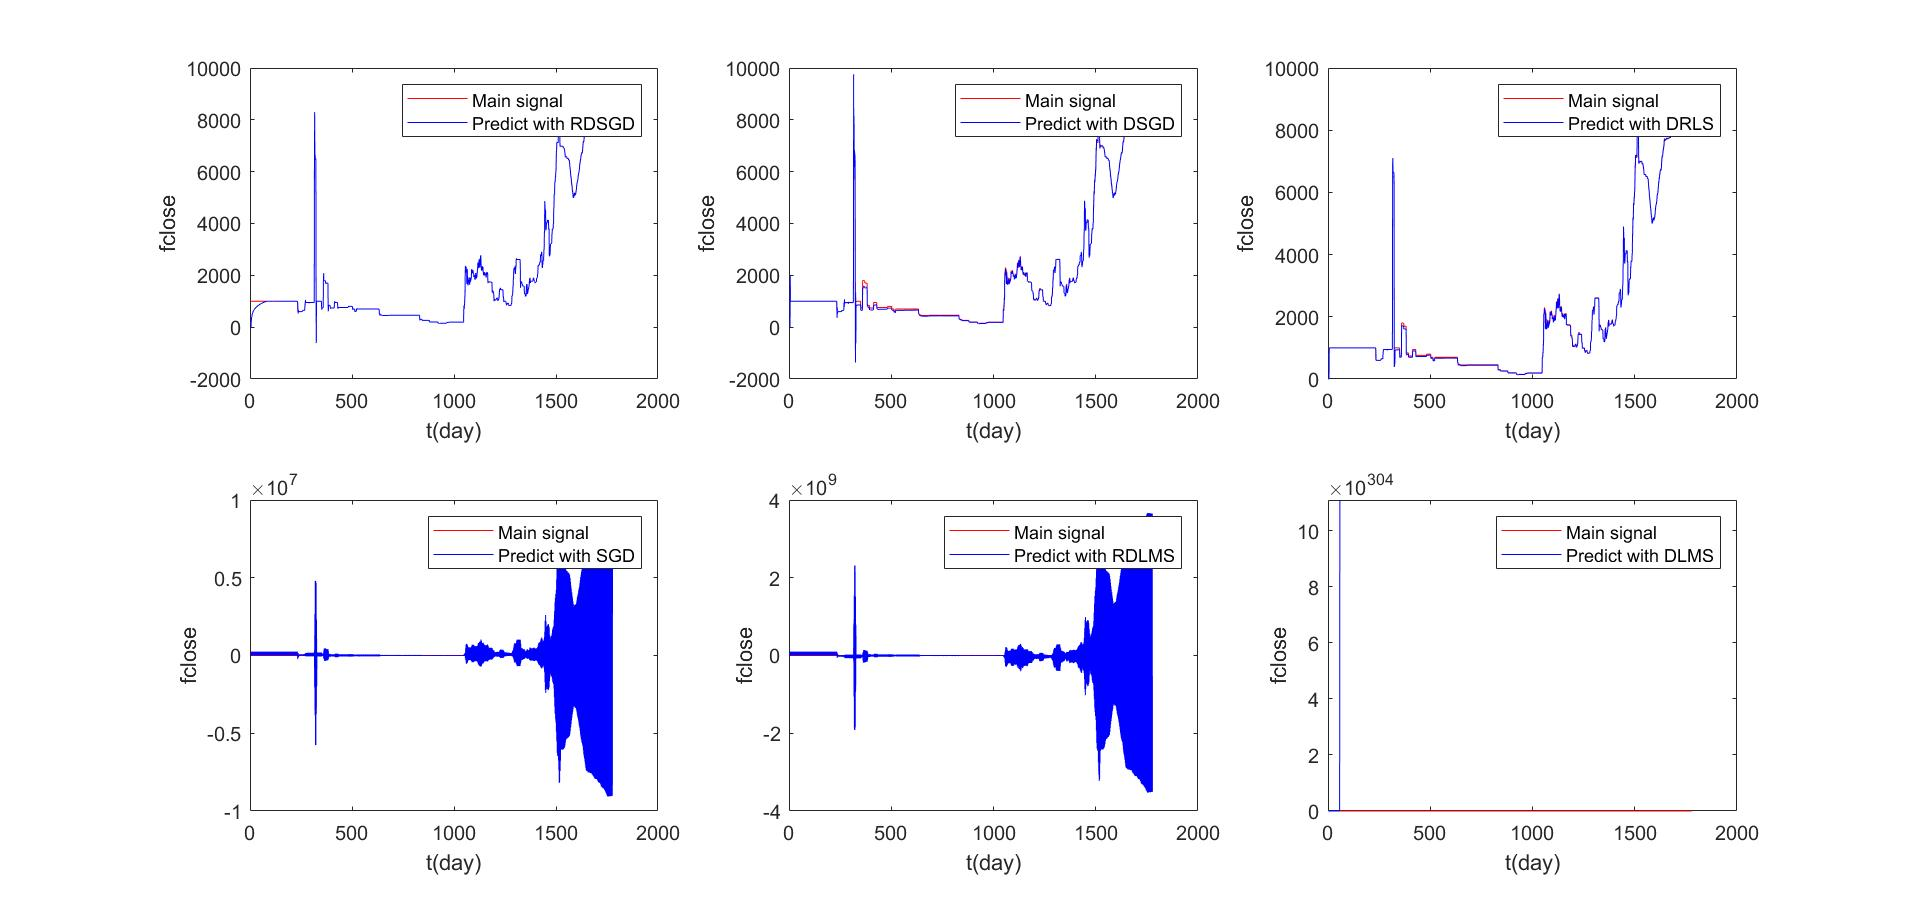
\includegraphics[width=16cm]{CompareFigs_6_Permit.jpg}
	\caption{مقایسه الگوریتم‌های یادگیری توزیع‌شده رویکرد \lr{FBSP} در پیش‌بینی سیگنال بازار سهام شرکت پرمیت}
	\label{PredictCompare2}
\end{figure*}

\begin{figure*}[!h]
	\centering
	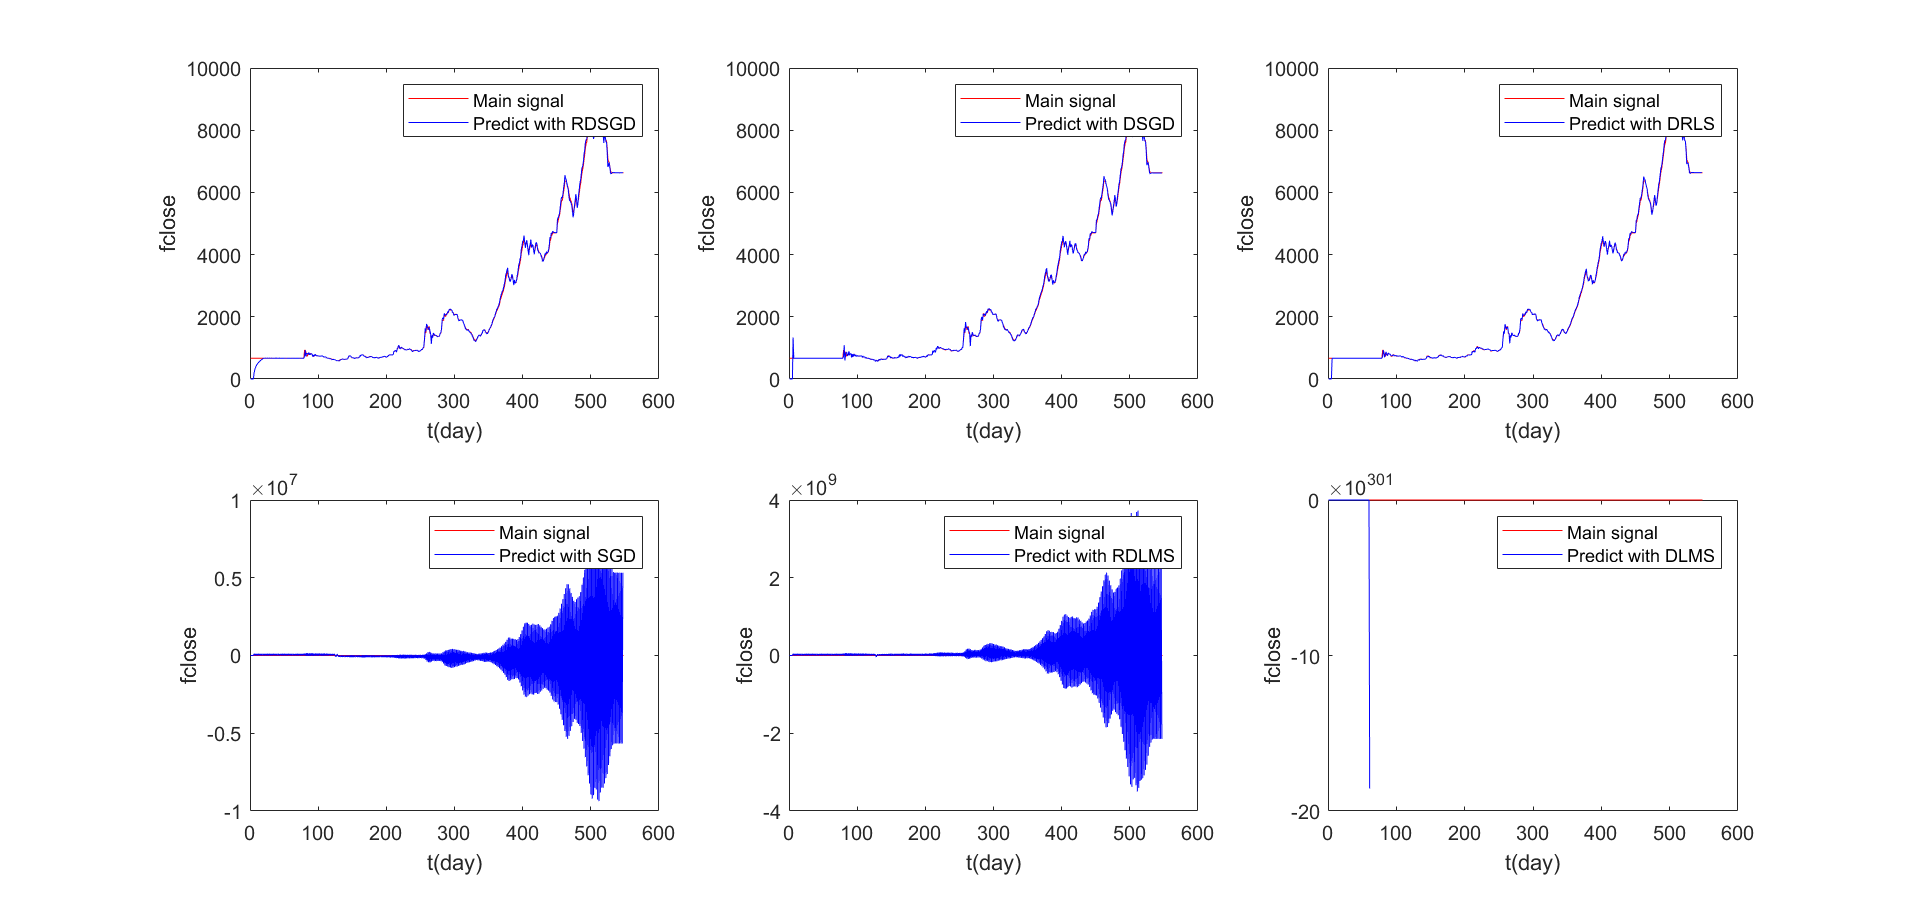
\includegraphics[width=16cm]{VMelat_Pre.png}
	\caption{مقایسه الگوریتم‌های یادگیری توزیع‌شده رویکرد \lr{FBSP} در پیش‌بینی سیگنال بازار سهام شرکت سرمایه گذاری ملت }
	\label{PredictCompare3}
\end{figure*}

\begin{figure*}[!h]
	\centering
	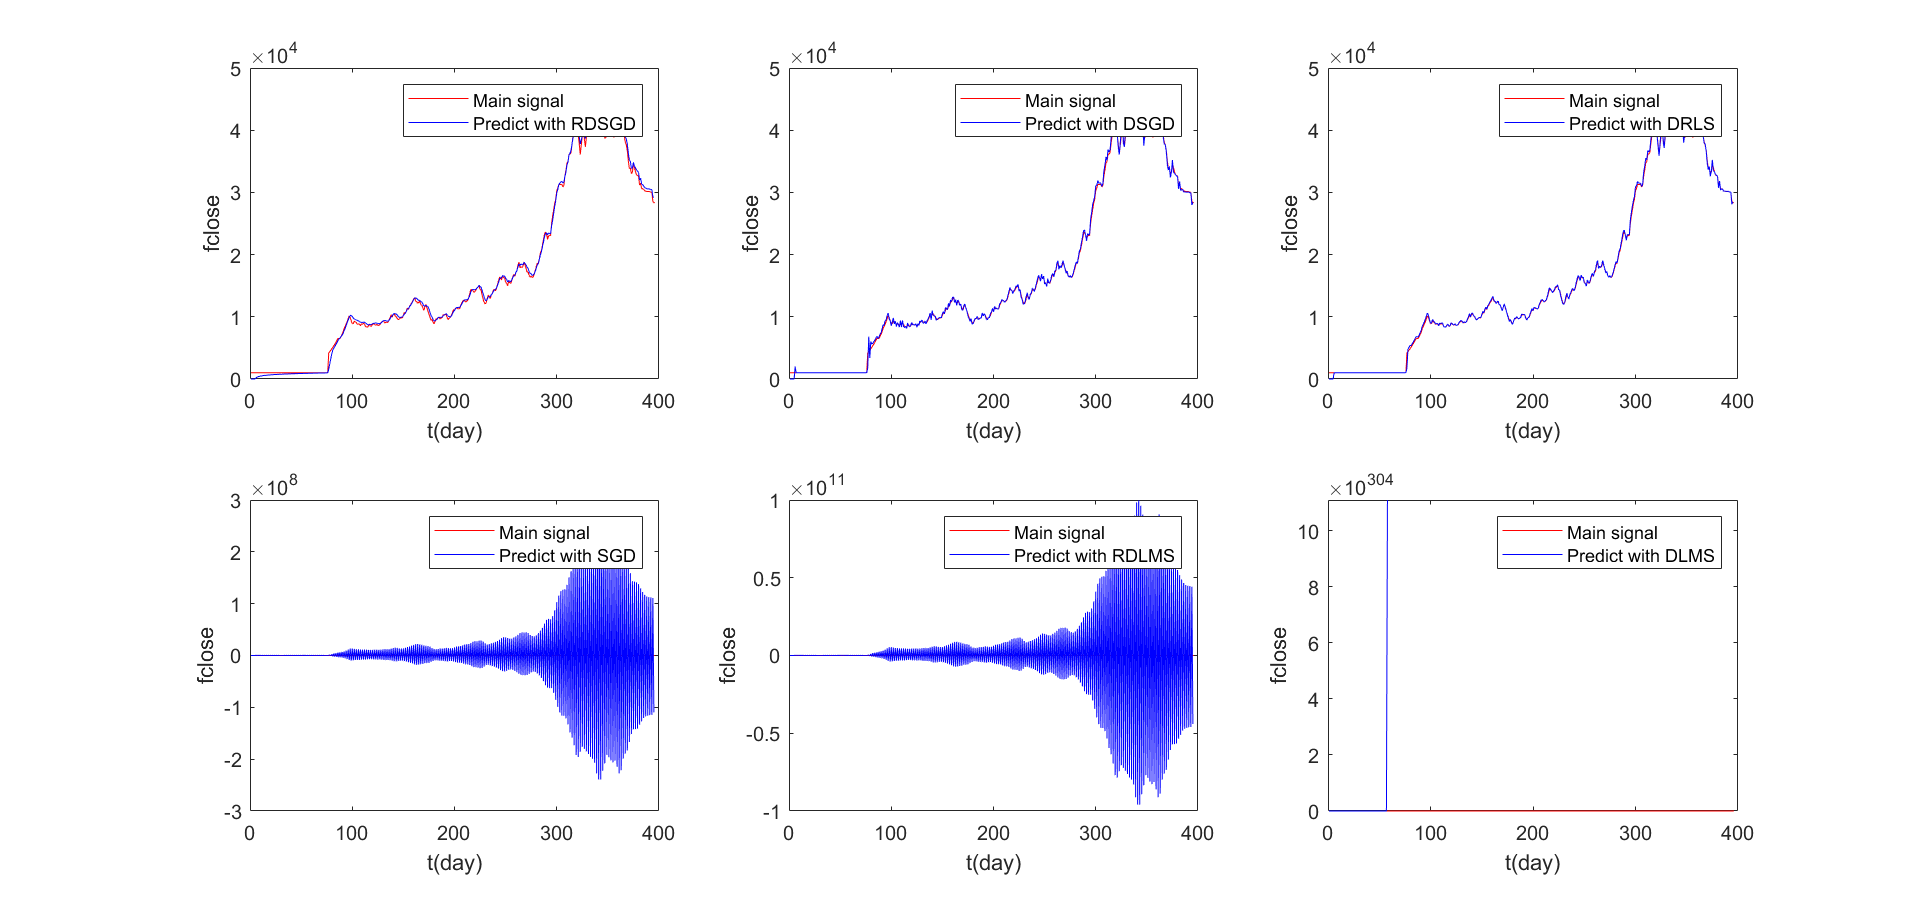
\includegraphics[width=16cm]{ZSharif_Pre.png}
	\caption{مقایسه الگوریتم‌های یادگیری توزیع‌شده رویکرد \lr{FBSP} در پیش‌بینی سیگنال بازار سهام شرکت کشت و صنعت شریف آباد}
	\label{PredictCompare4}
\end{figure*}

\section{خلاصه}
در این فصل، الگوریتم‌های پیشنهادی و رویکرد پیشنهادی روی مسائل شناسایی سیستم و پیش‌بینی داده‌های بورس آزمایش شدند. برای مقایسه با سایر روش‌ها چند معیار ارزیابی و چند روش مقایسه مورد استفاده قرار گرفت. در طی چندین آزمایش، عوامل متعدد و پارامترهای موثر بر کارایی رویکرد پیشنهادی مورد بررسی قرار گرفت. در اولین بررسی انجام شده، تاثیر الگوریتم یادگیری توزیع‌شده مبتنی بر \lr{SGD} بر سرعت همگرایی و دقت یادگیری در مساله بهینه‌سازی شناسایی سیستم نشان داده شد. در واقع الگوریتم پیشنهادی تاثیر چشم‌گیری در کاهش خطا در حالت پایدار داشت. در بررسی دیگر، تاثیر توابع زیان بر مقاومت الگوریتم یادگیری پیشنهادی در برابر انواع نویزهای گاوسی و غیرگاوسی و در انواع محیط‌های ایستا و غیرایستا مورد بررسی قرار گرفت و نشان داده شد که الگوریتم یادگیری پیشنهادی با تابع زیان شبه‌هابر (\lr{RDSGD}) مقاومت بهتری ارائه می‌دهد و نسبت به سایر الگوریتم‌های یادگیری با میانگین خطا کمتری در حالت پایدار همگرا می‌شود. 

رویکرد پیشنهادی \lr{FBSP} با استفاده از الگوریتم‌ یادگیری \lr{RDSGD} و منطقه‌بندی گره‌های شبکه توزیع‌شده، اهدافی چون مدیریت محیط‌های اجرایی ناهمگن، کاهش هزینه ارتباطات، کاهش زمان انتظار گره‌ها در طی فرآیند یادگیری و جلوگیری از مساله کندکننده‌ها با حفظ سرعت و دقت همگرایی را دنبال می‌کند. رویکرد پیشنهادی به دلیل منطقه‌بندی شبکه توانایی بالایی در کاهش هزینه ارتباطات و کاهش زمان انتظار گره‌ها برای شبکه‌های غیرخلوت دارد. در اولین آزمایش تاثیر مقدار پارامتر $qIter$ بر همگرایی، میانگین زمان انتظار و میانگین تعداد ارتباطات گره‌ها در محیط غیرایستا و در حضور نویزهای گاوسی، گاوسی آمیخته و آلفا پایدار مورد ارزیابی قرار گرفت و نشان داده شد که با افزایش مقدار پارامتر $qIter$ رویکرد پیشنهادی به میانگین خطا بالاتری همگرا شده اما در مقابل تعداد ارتباطات و زمان انتظار گره‌ها کاهش می‌یابد. به عبارتی میانگین خطا همگرایی رابطه معکوس با میانگین زمان انتظار گره‌ها دارد. رویکرد پیشنهادی به ازای پارامتر کنترلی $qIter=50$ در یک محیط غیرایستا قادر است باعث کاهش $36.73$ درصدی تعداد ارتباطات و کاهش $36.9$ درصدی زمان انتظار گره‌ها شود. این در حالی است که رویکرد پیشنهادی سبب افزایش تنها $13.38$ درصد در میانگین خطا همگرایی در حالت پایدار  شده است. در آزمایش دوم، رویکرد پیشنهادی از جنبه میانگین زمان انتظار و میانگین خطا همگرایی با سایر رویکردهای مشابه مورد مقایسه قرار گرفت و رویکرد پیشنهادی با پارامتر کنترلی $qIter=50$ به سایر رویکردها غلبه کرد. در آزمایشی دیگر، مقاومت رویکرد پیشنهادی در برابر محیط‌های اجرایی ناهمگن مختلف مورد بررسی قرار گرفت و نشان داده شده که رویکرد \lr{FBSP} از مقاومت بالایی در محیط‌های ناهمگن نسبت به رویکرد مشابه خویش \lr{PSP} دارد. در آزمایش آخر نشان داده شده که رویکرد پیشنهادی با الگوریتم یادگیری توزیع‌شده انتشاری \lr{RDSGD} در مساله پیش‌بینی داده‌های بورس نیز موفق است.


\chapter{نتیجه‌گیری}
\newpage
‎\renewcommand{\baselinestretch}{2}\normalsize‎
\label{Conclusion}

همانطور که در این رساله بیان کردیم، رویکرد یادگیری برای شبکه‌های تطبیقی توزیع‌شده ناهمگن طراحی و ارائه نشده است. سایر روش‌های یادگیری توزیع‌شده مطرح شده یا به صورت متمرکز پیاده‌سازی شده‌اند و یا شبکه را به صورت مجموعه‌ای از گره‌های همگن فرض کرده‌اند. هر کدام از این روش‌ها نقاط ضعفی دارند که در فصل‌های قبل بیان کرده‌ایم. در این فصل به بیان نتیجه‌گیری کل کار پرداخته می‌شود و در پایان نیر به بیان پیشنهادهایی در راستای ادامه این کار خواهیم پرداخت. 

\section{نتیجه‌گیری}
امروزه روش‌های موازی‌سازی و مدل‌های محاسباتی به دلیل افزایش حجم محاسبات و داده‌های پردازشی در بسیاری از زمینه‌ها و کاربردها توجه زیادی را به خود جلب نموده‌اند. همچنین با پیشرفت روز افزون تکنولوژی و قدرت‌های پردازشی متفاوت سیستم‌ها، فرایند یادگیری در شبکه‌‌ای از گره‌های پردازشی با محدودیت‌ها و چالش‌های مهمی مواجه خواهد بود. در یک شبکه تطبیقی توزیع‌شده، اگر عملیات محاسباتی برای گره‌ها سنگین باشد و یا داد‌های ورودی ذاتاً توزیع‌شده و سنگین باشند، مهمترین چالش در این نوع یادگیری، موازی‌سازی فرآیند آموزش و ایجاد یک مدل منسجم در کل شبکه است.  از آنجایی که موازی‌سازی بهتر است تحت یک ساختار و مدل مشخص و کارایی انجام شود، ارائه یک مدل محاسباتی موازی منطبق با ویژگی‌های شبکه‌های تطبیقی توزیع‌شده با قابلیت اجرای کارا در محیط‌های ناهمگن بسیار چالش برانگیز بوده اما دستیابی به آن هدفی بسیار ارزشمند است. 

مدل محاسباتی موازی \lr{BSP} مدلی مناسب برای شبکه‌های تطبیقی توزیع‌شده می‌باشد اما کلیه گره‌های شرکت کننده در فرایند یادگیری این شبکه در سطح یکسانی قرار دارند. از آنجایی که گره‌های شبکه ممکن است از لحاظ قدرت محاسباتی و پردازشی متفاوت باشند، مدل محاسباتی \lr{BSP} برای این حالت مناسب و کارا نمی‌باشد. از این رو در این رساله، به طراحی و ارائه مدل محاسباتی توسعه‌یافته‌ای به نام \lr{BSP} فدرالی پرداخته شد. طراحی چنین مدلی با هدف کاهش زمان انتظار گره‌ها در طول فرایند یادگیری و کاهش میزان ارتباطات با حفظ سرعت همگرایی و دقت یادگیری انجام شد. 

رویکرد یادگیری توزیع‌شده مبتنی بر مدل محاسباتی \lr{BSP} فدرالی ارائه شده از دو مرحله اصلی برون خط و برخط تشکیل شده است. در مرحله اول گره‌های شبکه در منطقه‌هایی مشابه خوشه‌بندی می‌شوند. در ساختار مدل محاسباتی توسعه یافته ارتباطات به منظور تبادل اطلاعات و همچنین همگام‌سازی‌های مانعی به منظور همگام‌شدن تخمین‌های گره‌ها در انتهای هر ابرگام بر اساس منطقه‌ها انجام می‌شود. در مرحله دوم فرایند یادگیری توزیع‌شده توسط گره‌های منطقه‌بندی‌شده به دو صورت منطقه‌ای و سرتاسری انجام می‌شود. از آنجایی که گره‌ها با قدرت پردازشی مشابه در یک منطقه قرار می‌گیرند، گره‌های کند دیگر مانع همگام‌سازی دیرهنگام گره‌های سریع‌تر نمی‌شوند. در ابرگام‌های منطقه‌ای، هر منطقه مستقل از سایر منطقه‌ها فرایند یادگیری را به صورت تطبیقی توزیع‌شده اجرا می‌کند. در ابرگام‌های سرتاسری، هر گره فرایند یادگیری را به صورت عادی و در سطح کل شبکه انجام می‌دهد. همین امر منجر به کاهش زمان انتظار گره‌ها در زمان اجرا فرایند تخمین پارامترها شد و همچنین منجر به کاهش تعداد ارتباطات و تبادل اطلاعات بین گره‌ها گردید. 

\section{پیشنهادات آتی}
اگر چه نتایج حاصل از این پژوهش رضایت‌بخش و قابل قبول می‌باشد، با این حال جنبه‌های جذاب و جالب توجهی پیش‌روی این زمینه پژوهشی وجود دارد. می‌توان مباحث امنیت داده‌ها را در این کار دخیل کرد و کار تحقیقاتی جدید را تعریف نمود. همچنین می‌توان رویکرد پیشنهادی را برای شبکه‌های عصبی عمیق استفاده کرد و آن را در این زمینه توسعه داد و راهکار موثری عرضه کرد. از سوی دیگر می‌توان مدل‌های محاسباتی دیگر را نیز به صورت فدرالی توسعه داد و نسخه‌های جدیدی از آنها برای کار بر روی داده‌های غیرمستقل با توزیع‌های متفاوت عرضه کرد.

\section{مقالات مستخرج از رساله}
با انجام این رساله، دو مقاله چاپ شده و یک مقاله ارسال شده از آن استخراج شده است. مقاله اول مربوط به الگوریتم یادگیری توزیع‌شده پیشنهادی می‌باشد که نتیجه آن چاپ یک مقاله در مجله \lr{Journal Signal Processing} با عنوان \lr{‌‌‌Convergence Behavior of Diffusion Stochastic Gradient Descent Algorithm} در سال 2021 شده است. مقاله دوم مربوط به مقاوم‌سازی الگوریتم یادگیری پیشنهادی و مساله پیش‌بینی سیگنال‌های بازار بورس می‌باشد که نتیجه آن چاپ یک مقاله در مجله \lr{Journal of Parallel and Distributed Computing} با عنوان \lr{A Distributed Learning based on Robust Diffusion SGD over Adaptive Networks with Noisy Output Data} در سال 2024 شده است. مقاله سوم مربوط به مدل محاسباتی پیشنهادی می‌باشد که به مجله \lr{Journal of IEEE Transactions on Parallel and Distributed Systems} ارسال شده است و تحت داوری است. 
%\renewcommand{\arraystretch}{2}
%\setlength{\tabcolsep}{25t}
\begin{table}[h]
	\centering
	\caption{\small{لیست مقالات مستخرج از رساله}}
	\footnotesize\rm
%	\resizebox{\textwidth}{!}{
	\begin{tabular}{|c|p{4cm}|p{4cm}|p{4cm}|c|}
		\hline
		ردیف&عنوان&نویسندگان&محل انتشار&تاریخ\\
		\hline
	1&\lr{‌‌‌Convergence Behavior of Diffusion Stochastic Gradient Descent Algorithm}&\lr{Fatemeh Barani, Abdorreza Savadi, Hadi Sadoghi Yazdi}&\lr{Journal Signal Processing}&2021\\
	\hline
	2&\lr{A Distributed Learning based on Robust Diffusion SGD over Adaptive Networks with Noisy Output Data}&\lr{Fatemeh Barani, Abdorreza Savadi, Hadi Sadoghi Yazdi}&\lr{Journal of Parallel and Distributed Computing}&2024\\
	\hline
	3&\lr{Federated Bulk Synchronous Parallel Model for Distributed Adaptive Networks}&\lr{Fatemeh Barani, Abdorreza Savadi, Hadi Sadoghi Yazdi}&\lr{Journal of IEEE Transactions on Parallel and Distributed Systems}&\lr{Submit}\\
		\hline
	\end{tabular}
%}
\end{table}

\section{خلاصه}
در این فصل تحلیل نتایج و نقاط قوت و ضعف رویکرد پیشنهادی بیان شده است و با توجه به نقاط ضعفی که در رویکرد پیشنهادی وجود دارد، پیشنهادهایی نیز برای مطالعات آینده بیان شد. همچنین مقالات مستخرج شده از این رساله آورده شده‌اند. 



\bibliographystyle{unsrt-fa}
\bibliography{ref}

\def\title{\large{واژه نامه فارسی به انگلیسی}}
\def\dic{ 
\persiangloss{فارسی}{English}
\persiangloss{ابرگام}{Super step}
\persiangloss{ابرگام منطقه ای}{Regional super step}
\persiangloss{ابرگام سراسری}{Global super step}
\persiangloss{اختلاف همگرایی وزن دار}{Weighted convergence difference}
\persiangloss{ارتباطات منطقه ای}{Regional communication}
\persiangloss{ارتباطات سراسری}{Global communication}
\persiangloss{استراتژی انتشاری}{Diffusion strategy}
\persiangloss{الگوریتم های مقاوم}{Robust algorithms}
\persiangloss{الگوریتم دیجسترا}{Dijkstra algorithm}
\persiangloss{اندازه گام}{Step size}
\persiangloss{بردار پارامتر}{Parameter vector}
\persiangloss{بردار وزن}{Weight vector}
\persiangloss{بردار وزن خطا}{Weight-error vector}
\persiangloss{پیش شرط}{Preconditioner}
\persiangloss{پیچیدگی محاسباتی}{Computational complexity}
\persiangloss{تابع هدف}{Objective function}
\persiangloss{تابع خطا/زیان}{Loss function}
\persiangloss{تابع خطا شبه-هابر}{Pseudo-Huber Loss Function}
\persiangloss{ترم تنظیم}{Regularization term}
\persiangloss{توزیع شده}{Distributed}
\persiangloss{حالت پایدار}{Steady-state}
\persiangloss{داده پرت}{Outlier}
\persiangloss{داده نویزی}{Noise data}
\persiangloss{رفتار همگرایی}{Convergence behavior}
\persiangloss{سناریو تک وظیفه ای}{Single-task scenario}
\persiangloss{سناریو چند وظیفه ای}{Multi-task scenario}
\persiangloss{شبکه}{Network}
\persiangloss{شبکه تطبیقی}{Adaptive Network}
\persiangloss{شبکه منطقه بندی شده}{Regionalized network}
\persiangloss{شباهت ساختاری}{Structural Similarity}
\persiangloss{شباهت محتوایی}{Content Similarity}
\persiangloss{شباهت ژاکارد}{Jaccard similarity}
\persiangloss{شعاع طیفی}{Spectral radius}
\persiangloss{شناسایی سیستم}{System identification}
\persiangloss{گام ترکیب}{Combination step}
\persiangloss{گام تطبیق}{Adaptation step}
\persiangloss{گراف ساختار-محتوایی}{Content-structural graph}
\persiangloss{ماتریس ترکیب}{Combination matrix}
\persiangloss{مانع همگام سازی منطقه ای}{Regional synchronous barrier}
\persiangloss{مانع همگام سازی سراسری}{Global synchronous barrier}
\persiangloss{محیط ایستا}{Stationary environment}
\persiangloss{محیط غیرایستا/متحرک}{non-Stationary environment}
\persiangloss{مرتبه یا اندازه فیلتر}{Filter order}
\persiangloss{منطقه بندی}{Regioning}
\persiangloss{منطقه}{Region}
\persiangloss{مدل محاسباتی موازی}{Model of parallel computation}
\persiangloss{نرخ همگرایی}{Convergence rate}
\persiangloss{نویز پایدار الفا}{ $\alpha$-stable noise}
\persiangloss{نویز تکانشی}{impulsive noise}
\persiangloss{نویز گوسی}{Gaussian noise}
\persiangloss{نویز گاوسی آمیخته}{Mixture Gaussian noise}
\persiangloss{نویز غیرگاوسی}{non-Gaussian noise}
\persiangloss{یادگیری توزیع شده}{Distributed learning}
\persiangloss{یادگیری فدرالی}{Federated learning}
}
\begin{center}
\title
\end{center}
\dic



\def\title{\large{اصلاحات به ‌کار رفته در پایان نامه}}
\def\dic{ 


\persiangloss{\lr{SGD}}{Stochastic Gradient Descent}
\persiangloss{\lr{GD}}{Gradient Descent}
\persiangloss{\lr{ITL}}{Information Theory Learning}
\persiangloss{\lr{LMS}}{Least Mean Square}
\persiangloss{\lr{RLS}}{Recursive Least Squares}
\persiangloss{\lr{ATC}}{Adapt-then-Combine}
\persiangloss{\lr{CTA}}{Combine-then-Adapt}
\persiangloss{\lr{MSD}}{Mean Square Deviation}
\persiangloss{\lr{MSE}}{Mean Square Error}
\persiangloss{\lr{ICS-cluster}}{Incremental Structural Content Clustering}
\persiangloss{\lr{FL}}{Federated Learning}
\persiangloss{\lr{BSP}}{Bulk Synchronous Parallel}
\persiangloss{\lr{SSP}}{Stale Synchronous Parallel}
\persiangloss{\lr{ASP}}{Asynchronous Parallel}
\persiangloss{\lr{FBSP}}{Federated Bulk Synchronous Parallel}
\persiangloss{\lr{MPI}}{Massage Passing Interface}
}
\begin{center}
\title
\end{center}
\dic


 \begin{latin}
\def\title{\large{Abstract}}
\def\keyword{\textbf{Keywords: }}
\def\abstracten{ 
Nowadays, distributed adaptive networks have attracted the attention of researchers in the field of distributed learning due to their high scalability, resistance to failures, and decentralization. The learning process of distributed algorithms must have a specific structure and be based on a parallel computing model so that the communication between parallel software and parallel hardware can be done easily. The parallel computing model \lr{BSP} can be easily applied to these networks; But in a heterogeneous environment, if barrier synchronization is applied in \lr{BSP}, the straggler problem occurs and the average idle time of nodes increases. In this thesis, in order to manage the heterogeneous environment, in the first step, using a content-structural clustering method, network nodes are regionalized. In the second step, a developed parallel computing model called federated \lr{BSP} or \lr{FBSP} is presented. The proposed computing model, like \lr{BSP}, consists of three important parts of calculation, communication, and barrier synchronization, with the difference that in \lr{FBSP}, there are two types of regional superstep and global superstep. Also, communication and barrier synchronization of proposed model are carried out at both regional and global levels. Two-level communication will reduce communication costs and two-level barrier synchronization will deal with the straggler problem and reduce the average idle time of nodes. In the next step, a distributed learning approach based on the \lr{FBSP} model was presented to solve the optimization problems. In order to robust the proposed approach against all type of noises and adapt to stationary and non-stationary environments, a distributed learning algorithm named \lr{RDSGD} based on stochastic gradient descent was introduced. Finally, an independent software tool named \lr{FBSPonMPI} is presented for developing distributed applications on the platform of adaptive networks in \lr{C} and Python, which is fast and independent of hardware. Analysis of the convergence and efficiency of the proposed approach in the mean state and the mean square state and the impact of random topology on the network and quantization error have been done. In order to confirm the obtained analytical results, the proposed approach has been compared with other approaches using a number of evaluation criteria. The FBSP model-based approach was evaluated on the optimization problem of system identification and stock market forecasting. The proposed approach is more resistant and consistent in the presence of different type of noises and in stationary and non-stationary environments than other methods. The obtained results show that the proposed approach has succeeded in reducing the average idle time by $36.9\%$ and reducing the average number of connections by $58\%$ while maintaining the convergence rate and learning accuracy.
}

\def\keyworden{Distributed Adaptive Networks, Distributed Learning, Parallel Computing Model, Federated Bulk Synchronous Parallel Computing Model, Regional Superstep, Global Superstep}



\begin{center}
\title
\end{center}
\abstracten

\keyword
\keyworden
\end{latin}
\def\thesistitlefa{Federated Bulk Synchronous Parallel Model for Distributed Adaptive Networks} ‌
\def\byfa{By:}
\def\authorfa{Fatemeh Barani}
\def\submitedforfa{Ph.D Dissertation}
\def\undersupervisionfa{Supervisor:}
\def\supervisorfa{Dr. Abdorreza Savadi}

\def\advisor{Advisor:}
\def\advisorname{Dr. Hadi Sadoghi Yazdi}

\def\datefa{2024} 
\def\facultyfa{Department of Computer Engineering\\Ferdowsi University of Mashhad}
\def\universityfa{Ferdowsi University of Mashhad}
\def\locationfa{Mashhad}



%---------------------------
% بسم الله الرحمن الرحیم

%---------------------------
% Thesis Title Farsi
\begin{latin}
\thispagestyle{empty}
\begin{titlepage}
\begin{center}

\includegraphics[scale=0.8]{logoen.png}\\
{\facultyfa}
\vskip 1.5cm
{\large\bfseries\submitedforfa}
\vskip 1.5cm
{\Large\thesistitlefa}
\vskip 1.5cm

{\byfa}
\vskip 1.2cm
{\Large\bfseries\authorfa}
\vskip 2cm
{\undersupervisionfa}
\vskip 1cm
{\Large\bfseries\supervisorfa}
\vskip 3cm
{\advisor}
\vskip 1cm
{\Large\bfseries\advisorname}
\vskip 3cm
{\large\datefa}
\vskip 0.5cm
%{\bfseries\large\facultyfa
%\vskip 0cm
%\universityfa
%\vskip 0cm
%\locationfa}
\end{center}
\end{titlepage}
\end{latin}


%------------------------------
% Abstract Fa Page
{
\thispagestyle{empty}
$ $
\vskip 1.5cm
\setlength\baselineskip{0.7cm}
%\begin{center}
%\Large\thesistitlefa
%\end{center}




}







\end{document}